%\documentclass[a4paper,12pt]{eskdtext} %размер бумаги устанавливаем А4, шрифт 12пунктов
\documentclass[a4paper,14pt]{scrartcl} %размер бумаги устанавливаем А4, шрифт 12пунктов
%\documentclass[14pt,a4paper,twoside]{report}
\usepackage[T2A]{fontenc}
\usepackage[utf8]{inputenc} %включаем свою кодировку: koi8-r или utf8 в UNIX, cp1251 в Windows
\usepackage[english,russian]{babel} %используем русский и английский языки с переносами
\usepackage{amssymb,amsfonts,amsmath,mathtext,cite,enumerate,float} %подключаем нужные пакеты расширений
\usepackage[dvips]{graphicx} %хотим вставлять в диплом рисунки?
%\usepackage{soul}
\usepackage[14pt]{extsizes}
\usepackage{longtable}
\usepackage{graphicx}
\usepackage{indentfirst}
\usepackage{enumerate}
\usepackage{xcolor}

\graphicspath{{../images/}} %путь к рисункам

%\linespread{1.5}

\usepackage[format=plain,labelformat=simple,labelsep=endash,figurename=\CYRR\cyri\cyrs\cyru\cyrn\cyro\cyrk]{caption}
\captionsetup{figurewithin=section} % картинки нумеруются относительно секций
\numberwithin{equation}{section} % нумерация формул внутри раздела
\numberwithin{table}{section}

\makeatletter
\renewcommand{\@biblabel}[1]{#1.} % Заменяем библиографию с квадратных скобок на точку:
\makeatother

\RequirePackage{lscape}

%\renewcommand\large{\@setfontsize\large{15.5}{17}}
%\renewcommand\Large{\@setfontsize\Large{16.5}{19}}
%\renewcommand\small{\@setfontsize\small{9}{9.5}}

\usepackage{geometry} % Меняем поля страницы
\geometry{left=2cm} % левое поле
\geometry{right=1cm} % правое поле
\geometry{top=2cm} % верхнее поле
\geometry{bottom=2cm} % нижнее поле

\renewcommand{\theenumi}{\arabic{enumi}} % Меняем везде перечисления на цифра.цифра
\renewcommand{\labelenumi}{\arabic{enumi}} % Меняем везде перечисления на цифра.цифра
\renewcommand{\theenumii}{\arabic{enumii}} % Меняем везде перечисления на цифра.цифра
\renewcommand{\labelenumii}{\arabic{enumi}.\arabic{enumii}.}% Меняем везде перечисления на цифра.цифра
\renewcommand{\theenumiii}{\arabic{enumiii}} % Меняем везде перечисления на цифра.цифра
\renewcommand{\labelenumiii}{\arabic{enumi}.\arabic{enumii}.\arabic{enumiii}.}% Меняем везде перечисления на цифра.цифра

\renewcommand{\baselinestretch}{1.5}

% redefine title and bibl
\addto\captionsrussian{\def\contentsname{Содержание}}
%\addto\captionsrussian{\def\bibname{Список литературы}}
\addto\captionsrussian{\def\refname{Список используемых источников}}
 % main tamplate

\begin{document}
\noindent\centerline{\bf{Московский государственный технический университет}}
\noindent\centerline{\bf{имени Н. Э. Баумана}}
\vspace{\baselineskip}
\vspace{\baselineskip}

\hfill На правах рукописи

\vspace{\baselineskip}
\vspace{\baselineskip}

\noindent\centerline{\bf{Никифоров Александр Александрович}}

\vspace{\baselineskip}
\vspace{\baselineskip}

\noindent\centerline{РАЗРАБОТКА АЛГОРИТМА ОЦЕНКИ ПАРАМЕТРОВ}
\noindent\centerline{СИГНАЛА В СИСТЕМАХ С КОДОВЫМ РАЗДЕЛЕНИЕМ КАНАЛОВ}

\vspace{\baselineskip}
\vspace{\baselineskip}

\noindent\centerline{Специальность 05.13.01. – Системный анализ, управление и обработка информации}

\vspace{\baselineskip}
\vspace{\baselineskip}

\noindent\centerline{Диссертация на соискание ученой степени}
\noindent\centerline{кандидата технических наук}


\vspace{\baselineskip}
\vspace{\baselineskip}
\noindent\centerline{\bf{ЧЕРНОВИК}}
\noindent\centerline{16.04.14}

\vspace{\baselineskip}
\vspace{\baselineskip}

\hfill{Научный руководитель -}

\hfill{к.т.н., Сидоркина Ю. А.}

\vfill
\noindent\centerline{Москва – 2014}

\pagenumbering{gobble}
\newpage
 % это титульный лист
%\input{diplom_task}

\pagenumbering{arabic}
\tableofcontents % это оглавление, которое генерируется автоматически
\newpage

%\addcontentsline{toc}{section}{ВВЕДЕНИЕ}
\section*{ВВЕДЕНИЕ}

Большое количество современных систем являются беспроводными. Простота развертывания, мобильность, относительно низкая
стоимость - вот основные преимущества беспроводных систем. Количество мобильных устройств (телефоны, планшетные компьютеры
и т.д.) с каждым годом стремительно растет, только мобильных телефонов в 2011 году было 5.6 миллиарда и покрывало 79.86\%
\cite{wiki_mobilenum} населения земли. Технологии беспроводной связи глубоко проникли во все сферы жизни общества:
обеспечение безопасности с помощью RFID датчиков, предоставление доступа в интернет по технологиями 3G, WiFi, 
сотовая связь по различным технологиям (GSM, CDMA, DAMPS). Некоторые из этих систем строятся на основе методики
расширения спектра, которая отвечает современным требованиям по мощности сигнала, а так же по безопасности передаваемых
данных. В основе таких систем лежат шумоподобные (широкополосные) сигналы - ШПС. Вместе с тем растут требования к таким
системам. Применение ШПС ставит ряд специфических задач по обработке информации, обусловленных особенностями ШПС.
Свойства характерные для ШПС, выгодно отличают данный класс систем от класса узкополосных систем, но с другой стороны
оборачивается усложнением методов обработки ШПС.

Внедрение новых технологий требует увеличение полосы частот. Разнообразие технологий беспроводной передачи данных среди
гражданских и военных систем ведет к перегрузке каналов связи и все более высоким требованиям к скорости передачи
данных. С учётом данных требований применение систем передачи информации с ШПС становится все более востребованным.

Принимая во внимание географические размеры России и стратегическую важность обладания собственными системами спутникового
позиционирования, правительство Российский Федерации уделяет особое внимание разработке собственной системы
глобального спутникового позиционирования ГЛОНАСС. Обладание собственными технологиями системы спутниковой навигации (СНС), государство может обезопасить
себя в случае военных конфликтов от ограничения применения американской системы СНС Navstar GPS в зоне конфликта.

Разработка систем, позволяющих работать с несколькими различными СНС, позволит повысить точность определения координат
в сложных условиях города. Сложность детектирования сигнала и определения координат обусловлена наличием плотной
застройки многоэтажными зданиями. В городских условиях задача подавления интерференционной помехи становится особенно
актуальной. Спектр интерференционной помехи не является белым, а фильтрация и компенсация цветного шума
требует разработки специальных алгоритмов.

Новые цифровые процессоры позволяют применять подходы, которые еще 10-15 лет назад были бесперспективными.
В данной работе развиваются подходы на основе построения параметрической модели ШПС. Невозможность использования
методов требующих вычислений с высокой точностью в приемниках реального времени
10-15 лет назад была обусловлена слабой производительностью процессоров и микроконтроллеров, а так же существенной
стоимостью процессоров с модулем для операций с числами с плавающей точкой. Современное развитие цифровых технологий делает 
возможным применение параметрических методов оценки спектра взамен традиционного подхода основанного на непараметрического
анализа спектра.

Основа теории систем связи с ШПС была заложена в работах В.А. Котельникова и К. Шеннона.
России в этой области занимались В.И. Борисов, В.Б. Пестряков, В.И. Журавлев, М.И. Жодзишский, Б.И. Шахтарин, Л.Е.  Варакин, В.Е. Гантмахер и др.

Изначально методы расширенного спектра применялись при разработке военных систем управления и связи \cite{sklyar}.
К концу второй мировой войны расширение спектра применялось в радиолокации для борьбы с преднамеренными помехами, а
в последствии развитие данной технологии объяснялось желанием создать помехоустойчивые системы связи.
В конце 40-х-начале 50-х годов прошлого века Мортимер Рогофф, сотрудник Международной Телефонной и Телеграфной Корпорации (США) (ITT),
провёл эксперимент по передаче информации при помощи псевдошумового сигнала \cite{sklyar}, среди отечественных ученых
в середине 30-х годов прошлого века работу об основах кодового разделения каналов написал Д.В. Агеев.
Первые разработки таких систем относились к военным отраслям. Данный факт объясняется рядом особенностей, которыми обладают
сигналы с расширенным спектром, в числе которых — сложность перехвата заложенной в них информации,
высокая помехоустойчивость, а также трудность обнаружения факта работы передатчика. В процессе исследований расширенному спектру
нашлось и другое применение - снижение плотности энергии, высокоточная локация, использование при множественном доступе
\cite{sklyar}

Системы связи с широкополосными сигналами занимают особое место. Их особенные свойства выделяют данный класс из других систем
связи. Высокая помехозащищенность при действии сильной помехи, кодовое разделение большого количества абонентов, прием
информации с высокой достоверностью - отличительные особенности широкополосных система. Эти черты были известно, но
уровень элементной базы и низкий уровень помех не позволяли получить развития системам данного класса. Однако развитие
элементной привело к широкому распространению данного вида сигналов. В настоящее они применяются в системах спутниковой навигации,
системах сотовой связи и др \cite{varakin-book}.

Отношение сигнал/шум (ОСШ) на входе приемника может быть очень низким. Для обеспечения высокой помехозащищенности 
в таких случаях используются ШПС с большими и сверхбольшими базами.

К созданию сложных широкополосных сигналов (СШС) привело решение ряда проблем при развитии систем передачи данных.
Первая проблема встала при разработке новых радиолокационных система. Для дальнейшего развития требовалось
решить несколько противоречий: требование высокой разрешающей способности по дальности и дальностью обнаружения
целей в импульсных РЛС, требование точного измерения скорости и высокое разрешение по дальности, требование
увеличить дальность при ограничении пиковой мощности \cite{gantmaher-book}. Решение данных задач было предложено
Ф. Вудвардом. Им было показано, что дополнительным параметром является форма сигнала. Длительность сигнала
может быть больше - настолько больше, насколько это необходимо для обеспечения энергетических требований, а требование
разрешения по дальности и точности измерений определяются шириной полосы сигнала. Данные требования обеспечивается
путем сжатия импульса на стороне приемника. Вудворд сформулировал принципы: произведение эффективной полосы частот
радиосигнала на его длительность должен быть существенно больше единиц ${FT>>1}$, внутренняя структура сигнала
должна быть такой, чтобы обеспечить возможность приемнику сжатие распределенного во времени сигнала в короткий импульс,
соответствующий полосе ${F}$ \cite{gantmaher-book}.

В \cite{gantmaher-book} показана связь пропускной способности канала с понятием ШПС. При ${R_e<<1}$ можно записать:
\begin{center}
\begin{equation}
	\label{eq:shennon_cdma}
	FT = \frac{1}{\log(1+R_e)},
\end{equation}
\end{center}
где ${R_e}$ - ОСШ, ${F}$ - эффективная полоса частот, ${T}$ - длительность.

Стоить отметить, что при ${R_e<<1}$, левая часть выражения \ref{eq:shennon_cdma} стремится к бесконечности, а значит
ШПС позволяет обеспечить теоретически неограниченную достоверность передачи информации. Второе важное свойство
ШПС, следующее из \ref{eq:shennon_cdma} - способность работать "под шумами". Что обеспечивает скрытность
передачи информации, а с другой высокую степень уплотнения каналов связи и, как следствие, решение современных проблем
с перегруженностью каналов связи.

В данной работе будет рассматриваться ШПС модулированный ПСП на основе двоичной рекуррентной последовательности.
Для выделения данных из потока необходимо иметь точно синхронизированную копию ПСП, которая была использована
при модулировании сигнала на передающей стороне. Для достижения синхронизма на стороне приемника необходимо
устранить неопределенность в двух областях: неопределенность по частоте и неопределенность по фазе (задержке) ПСП.
Неопределенность по фазе ПСП обусловлена неопределенностью в расстоянии между передатчиком и приемником. Неопределенность
по частоте обусловлена в первую очередь допплеровским эффектом, а так же нестабильностью опорных генераторов в
передатчике и приемнике. После устранения неопределенности по частоте для достижения точной синхронизации
начинается процесс слежения за частотой. Неопределенность по фазе ПСП устранить, не используя полный перебор,
невозможно в силу корреляционных свойств ПСП. Таким образом можно заключить, что задача быстрого и эффективного
поиска и оценки параметров ШПС является актуальной.

В данной работе рассматривается подход программного приемника (Software Defined Receiver - SDR)
\cite{akos-book, grayver-book, pany-book} для оценки параметров ШПС. Как уже было отражено выше, ШПС применяется во
многих системах. В данной работе для полунатурного эксперимента будет рассматриваться сигнал СНС Navstar GPS. Данная система передачи 
информации использует ПСП Голда \cite{gold-ieee} для модулирования сигнала.

Традиционные подходы к реализации приемника СНС Navstar GPS отражены в \cite{akos-book, tsui}. 

Популярность и распространенность данной системы стимулирует исследования в области детектирования
и оценки частоты ШПС сигналов.

Существуют исследования в области применения теории хаоса - детектирование и оценка
частоты ШПС с применением осциллятора Дуффинга \cite{chaos_cambridge, chaos_chen, chaos_huang, chaos_wang}. Преимуществом
данного подхода является то, что свойства осциллятора позволяют детектировать сигналы с экстремально низким ОСШ. В то же
время, на данный момент никто не предложил цифровое представление осциллятора Дуффинга, а это затрудняет использование данного подхода
в реальных приемниках. Таким образом данное направление является в настоящее время больше теоретическим, чем практическим.

В работах \cite{hos_petropulu, hos_zhao} предложено использовать статистики высоких порядков для подавления шума и детектирование
сигналов с низким уровнем ОСШ.

Более традиционные подходы для детектирования и оценки параметров ШПС сигналов с низким уровнем ОСШ рассмотрены в монографии \cite{ziedan-book}.
В данной монографии рассматриваются как методы детектирования и оценки параметров ШПС, основанные на когерентном накоплении, так и эффективные
системы слежения за частотой и фазой ПСП.

{\bf{Добавить ЦЕЛИ И ЗАДАЧИ}}

%%%%%%
\paragraph{Постановка задачи оценки параметров сигнала с расширенным спектром.}
В данной работе рассматриваются задачи повышения рабочих характеристик приемников ШПС, поэтому целесообразно отразить основные модули этой системы 
на примере СНС Navstar GPS - рисунок \ref{pic:sec1_gnss_system}.
\begin{figure}[H]
\center\scalebox{1}{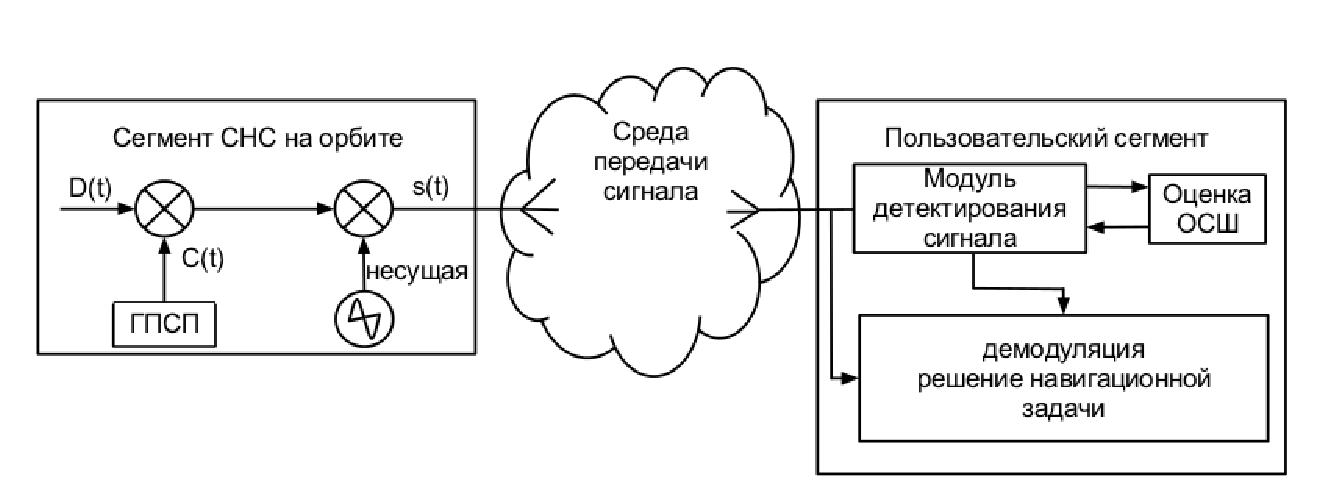
\includegraphics[width=1\linewidth]{sec1gnss_system.eps}}
\caption{структутраная схема СНС GPS}
\label{pic:sec1_gnss_system}
\end{figure}

В систему СНС Navstar GPS входят космический сегмент, наземный сегмент (на рисунке \ref{pic:sec1_gnss_system} не
отражен), а так же пользовательский сегмент. В космический сегмент входит спутниковая группировка, в 
наземный - станции управления, в пользовательский - все устройства принимающие сигнал от СНС GPS.

\paragraph{Модель сигнала и помех.}
В системе СНС Navstar GPS применяется ШПС.
Система передачи информации считается системой с расширенным спектром в следующих случаях \cite{sklyar}:
\begin{enumerate}
	\item Используемая полоса значительно шире минимальной, необходимой для передачи данных.
	\item Расширение спектра производится с помощью так называемого расширяющего сигнала (ПСП),
		который не зависит от передаваемой информации.
	\item Восстановление исходных данных ("сужение спектра") осуществляется путем сопоставления полученного
		сигнала и синхронизированной копии расширяющего сигнала (ПСП)
\end{enumerate}

Так же подобные сигналы называют:
\textquotedblleftсложными\textquotedblright,
\textquotedblleftшумоподобными\textquotedblright,
\textquotedblleftпсевдослучайными\textquotedblright,
\textquotedblleftсложными-дискретными\textquotedblright,
\textquotedblleftдискретно-кодированными\textquotedblright,
\textquotedblleftортогональными (квазиортогональными)\textquotedblright,
\textquotedblleftоптимальными дискретными\textquotedblright
\cite{gantmaher-book}.

Каждое название ставит акцент на определенной характеристике сигнала. В данной работе я буду оперировать термином
широкополосный сигнал - ШПС. ШПС можно определить как \cite{gantmaher-book, varakin-book}:
\begin{center}
\begin{equation}
	\label{eq:ss_signal}
	1 << FT = B,
\end{equation}
\end{center}
где: ${B}$ - база сигнала, ${F}$ - эффективная ширина спектра, а ${T}$ - длительность.
Неточность этого определения рассмотрена в \cite{gantmaher-book}, так же там даны ссылки на другие источники
разделяющие критику данного определения. Для данной работы критика, рассмотренная в приведенных источниках,
принципиального значения не имеет.

%%%%%%
\paragraph{Классическая постановка задачи оценки параметра.}
Из литературы по теории автоматических систем, например \cite{pugachev} (глава 10.1), известна классическая постановка
задачи задачи теории оптимальных систем. "На практике часто приходится решать задачу проектирования системы, когда
требуется определить характеристики системы таким образом, чтобы она имела наибольшую точность при данных условиях.
Систему обеспечивающую наибольшую возможную точность с какой-нибудь определенной точки зрения среди всех систем
заданного класса, обычно называют оптимальной" \cite{pugachev}.

В одной из постановок данной задачи \cite{pugachev} (глава 10.1), система считается полностью неизвестной
и требуется определить ее оператор так, чтобы она была оптимальной с точки зрения принятого критерия качества. Эта
задача сводится к определению с наибольшей возможной точностью некоторых параметров, от которых зависит принимаемый
сигнал. Но при этом важно учитывать не только точность, но и другие факторы, так как проектируемая система должна
удовлетворять многим, часто противоречивым требованиям. В виду приведенных факторов, обычно представляет собой
ряд компромиссных решений, удовлетворяющих всем предъявляемым к системе требованиям.

Точность автоматической системы обычно характеризуется математическим ожиданием и дисперсией ее ошибки.
Математическое ожидание представляет собой систематическую ошибку системы в данных условиях, а дисперсия
характеризует уровень случайных ошибок \cite{pugachev} (глава 10.2). Так как в различных условиях работы
системы, которые встречаются случайно систематическая ошибка тоже является случайной, за критерий качества
системы при ее проектировании обычно принимают второй начальный момент ошибки - математическое ожидание
квадрата ошибки:
\begin{center}
\begin{equation}
	\label{eq:stat_err_prob}
	\eta = M[e^2(t)]
\end{equation}
\end{center}
Положительный квадратный корень из этой величины называют средней квадратичной ошибкой системы. Таким образом,
оптимальной системой обычно считают такую систему, которая имеет минимальную среднюю квадратичную ошибку.

Критерий минимума средней квадратичной ошибки является простейшим с математической точки зрения и обычно приводит
к наиболее простым методам определения оптимальных систем. Однако далеко не во всех задачах он может служить мерой
качества системы. Поэтому нельзя ограничиваться методами нахождения оптимальных систем по критерию минимума средней
квадратичной ошибки.

В случаях, когда необходимо проектировать следящую систему, приходится учитывать возможность срыва слежения,
который заключается в том что система перестает работать, если ее ошибка превосходит по абсолютной величине некоторый
уровень. При проектировании таких систем целесообразно принять за критерий качества вероятность срыва слежения. При
этом оптимальной считается такая система, которая обеспечивает минимум вероятности срыва слежения. Если срыв слежения
происходит в случае, когда абсолютная величина ошибки превосходит уровень $a$, то критерий минимума вероятности ошибки
слежения можно представить \cite{pugachev} (глава 10.2):
\begin{center}
\begin{equation}
	\label{eq:prob_lost_signal}
	p = P(e(t) > a) = min
\end{equation}
\end{center}

%%%%%%
\paragraph{Введение обозначений.}
В диссертации рассматривается сигнал с расширенным спектром полученный методом "прямой последовательности".
Данный метод заключается в том, что гармоническая несущая сигнала модулируется высокоскоростным (широкополосным)
расширяющим сигналом (ПСП). 

Несущее колебание с частотой ${\omega_0}$  модулируется данными ${d(t)}$ , а также высокоскоростной ПСП ${g(t)}$, полученной методом "прямой последовательности".
СПИ Navstar GPS осуществляется двоичная фазовая модуляция (ДФМ или 2-ФМ), а значит ${d(t)}$  и ${g(t)}$  - потоки антиподных импульсов \{-1, 1\}.
Таким образом сигнал на выходе модулятора может быть представлен \cite{shahtarin_sync}:
\begin{equation}
	\label{eq:cdma_eq}
	s(t)=Ad(t)g(t)\cos{(\omega_{0}t)},
\end{equation}
где ${d(t)}$- информационный бит, а ${g(t)}$ - ПСП представляет собой фазовый сдвиг  ${0, \pi}$.

В реальных СПИ сигнал на приемник поступает одновременно от нескольких источников, присутствует неопределенность по частоте, а также аддитивный белый шум (АБГШ).
В приемнике после оцифровки сигнала получаем смесь:
\begin{equation}
	\label{eq:cdma_strip_eq}
	x(m)=\sum_{k=1}^{N}\left( A_k g(m + \tau_k)\exp{\left[j \left( \tilde{\omega}_{k}m + \phi_k(m)\right)\right]} \right) + n(m),
\end{equation}
где  ${k}$ - относительный номер источника сигнала, ${N}$ - количество доступных источников сигнала, модулированных ПСП одного семейства,
${m}$ - индекс соответствующий времени, ${\tilde{\omega}_{k}}$  – относительная частота, соответствующая ${\omega_0}$,
${\tau_k}$ - задержка модулирующей ПСП в точке приема, ${\phi_k(m)}$ - случайная начальная фаза, ${n(m)}$ - аддитивный белый гауссов шум (АБГШ). 

Следует отметить, что при оценке фазы сигнала с номером ${k}$  интерференцией являются сигналы:    .
\begin{equation}
	%\label{eq:cdma_interference}
	\{n \ne k, n \in [1,N]\}
\end{equation}

%%%%%%
\paragraph{Алгоритмы оценки параметров широкополосного сигнала сигнала.}
Алгоритм реализующий метод максимального правдоподобия - последовательный коррелятор. Данный подход реализуется в аппаратных приемниках.
Аппаратный приемник позволяет реализовать параллельно несколько последовательных корреляторов и вести оценку параметров
СПИ с ШПС параллельно.

Данный алгоритм в некоторых источниках так же называется согласованным фильтром. В \cite{sklyar} рассмотрены нюансы этих двух понятий.
В данной работе используется понятие последовательный коррелятор. Работа коррелятора описывается математической операцией
корреляции \ref{eq:serial_corr}. Сигнал коррелируется с локальной копией и на выходе коррелятора получается значение, отражающее
степень совпадения сигналов. Не трудно представить, что сигнал с хорошими корреляционными свойствами должен обладать высоким значением
корреляции когда сигналы синхронизированы и минимальным значением в любом другом случае (фаза ПСП не выровнена - отсутствие сигнала).
\begin{equation}
	\label{eq:serial_corr}
	y(n)=\sum\limits_{m=0}^{N-1}{x(m)h(n+m)},
\end{equation}
где ${x(m)}$ - принятая смесь, а ${h(n)}$ не импульсная характеристика системы, а локальная копия сигнала.

%%%%%%%%
% DFT

Вычисление циклической свертки через дискретное преобразование Фурье (ДПФ) - достаточно популярный метод
в программных приемниках, так как позволяет существенно уменьшить количество операций при вычислении. Но, как показано
в \cite{tsui, oppenheim}, можно достаточно просто перейти от свертки к циклической корреляции. Так как этот метод является самым
популярным в программных приемниках стоит его представить.
Свертка может быть представлена как:
\begin{equation}
	\label{eq:fft_conv}
	y(n)=\sum\limits_{m=0}^{N-1}{x(m)h(n-m)}
\end{equation}

Стоит отметить, что в \ref{eq:fft_conv} сдвиг во времени является циклическим, поскольку дискретные операции являются циклическими.
Возьмем ДПФ от \ref{eq:fft_conv}
\begin{center}
\begin{eqnarray}
	\label{eq:fft_conv_fft}
	Y(k) & = & \sum\limits_{n=0}^{N-1}\sum\limits_{m=0}^{N-1}{x(m)h(n-m)e^{(-j2\pi{kn})/N}}=\nonumber \\
	& = & \sum\limits_{m=0}^{N-1}{x(m)}[\sum\limits_{n=0}^{N-1}h(n-m)e^{(-j2\pi{(n-m)}k)/N}]e^{(-j2\pi{m}k)/N}=\\
	& = & H(k)\sum\limits_{m=0}^{N-1}e^{(-j2\pi{m}k)/N} = X(k)H(k)\nonumber 
\end{eqnarray}
\end{center}
Из уравнения \ref{eq:fft_conv_fft} легко видеть, что это не линейная свертка. В линейной свертке для входного сигнала размером в ${N}$ точек,
результат будет из ${2N-1}$ точек. А в уравнении выше, результатом является всего ${N}$ точек.
Это проявление циклической природы ДПФ.

Алгоритм оценки не использует свертку, он использует корреляцию, которая отличается от свертки. Корреляция
между $x(n)$ и $h(n)$ записывается выражением \ref{eq:serial_corr}:
Единственным отличаем между \ref{eq:serial_corr} и \ref{eq:fft_conv} является знак перед $m$ в ${h(n+m)}$.
В случае оценки параметра ШПС, $h(n)$ является локальной копией сигнала, а не импульсной характеристикой.
Произведем ДПФ над $z(n)$:
\begin{center}
\begin{eqnarray}
	\label{eq:fft_corr_fft}
	Z(k) & = & \sum\limits_{n=0}^{N-1}\sum\limits_{m=0}^{N-1}{x(m)h(n+m)e^{(-j2\pi{kn})/N}}=\nonumber \\
	& = & \sum\limits_{m=0}^{N-1}{x(m)}[\sum\limits_{n=0}^{N-1}h(n+m)e^{(-j2\pi{(n+m)}k)/N}]e^{(j2\pi{m}k)/N}=\\
	& = & H(k)\sum\limits_{m=0}^{N-1}e^{(j2\pi{m}k)/N} = X(k)H^{-1}(k)\nonumber 
\end{eqnarray}
\end{center}
где ${X^{-1}(k)}$ - обратное ДПФ. Уравнение \ref{eq:fft_corr_fft} можно записать как:

\begin{equation}
	\label{eq:fft_corr_fft_rev}
	Y(k) = \sum\limits_{n=0}^{N-1}\sum\limits_{m=0}^{N-1}{x(n+m)h(m)e^{(-j2\pi{kn})/N}}=X^{-1}(k)H(k)
\end{equation}

Если сигнал $x(n)$ действительный, то $x(n) = x^*(n)$, где ${^*}$ - операция комплексного сопряжения. Используя данное соотношение,
значение $Z(k)$ может быть записано:
\begin{equation}
	\label{eq:fft_magnitude}
	|Z(k)|=|H^*(k)X(k)|=|H(k)X(k)^*|
\end{equation}
Данное соотношение может быть использовано для нахождения значения циклической корреляции между входным сигналом и 
локальной копией.

%%%%%%%%
% Chaos 
Оценка параметров СПИ с ШПС (в частности сигналов системы Navstar GPS) с помощью осциллятора Дуффинга
достаточно новое направление в исследованиях по данной тематике. В данной области опубликовано несколько работ, в частности \cite{chaos_chen, chaos_cambridge, chaos_huang, chaos_song}.
Так же является интересной более ранняя статья не рассматривающая GPS \cite{chaos_wang}.
Осциллятор Дуффинга с гармоническим внешним воздействием может быть описан уравнением:
\begin{center}
\begin{equation}
	\label{eq:duffing}
	mx'' + cx' + k_{1}x + k_{2}x^3 = F_{0}\cos(\omega{t}),
\end{equation}
\end{center}
где $m$ - масса, $c$ - коэффициент диссипации, $x$ - состояние осциллятора, $k_1$ и $k_2$ - линейный и нелинейный коэффициенты соответственно,
$F_{0}\cos(\omega{t})$ - внешнее воздействие.

Подробно уравнение \ref{eq:duffing} рассмотрено в \cite{chaos_neimark_landa}.
Для использования осциллятора Дуффинга с целью оценки параметров ШПС была предложена усовершенствованная форма \cite{chaos_song, chaos_chen}:
\begin{center}
\begin{equation}
	\label{eq:duffing_gps}
	x'' +cx' - x^3 + x^5 = \gamma\cos(\omega{t}) + (\gamma_{x}\cos(\omega_{x}) + n(t))
\end{equation}
\end{center}

Перепишем динамическую систему \ref{eq:duffing_gps} в виде:
\begin{center}
\begin{equation}
	\label{eq:duffing_gps_2}
	\left\{
	\begin{aligned}
		y(t) & = x'(t) \\
		y'(t) & =  -cx' + x^3 - x^5 + \gamma\cos(\omega{t}) + (\gamma_{x}\cos(\omega_{x}) + n(t)),
	\end{aligned}
	\right.
\end{equation}
\end{center}
где ${n(t)}$ - АБГШ.

Пример фазового портрета при ${\omega=\omega_{x}}$ изображен на рисунке \ref{pic:duffing_sync},
фазовый портрет хаоса расположен на рисунках \ref{pic:duffing_chaos1}, \ref{pic:duffing_chaos2}
\begin{figure}[H]
	\center\scalebox{0.5}{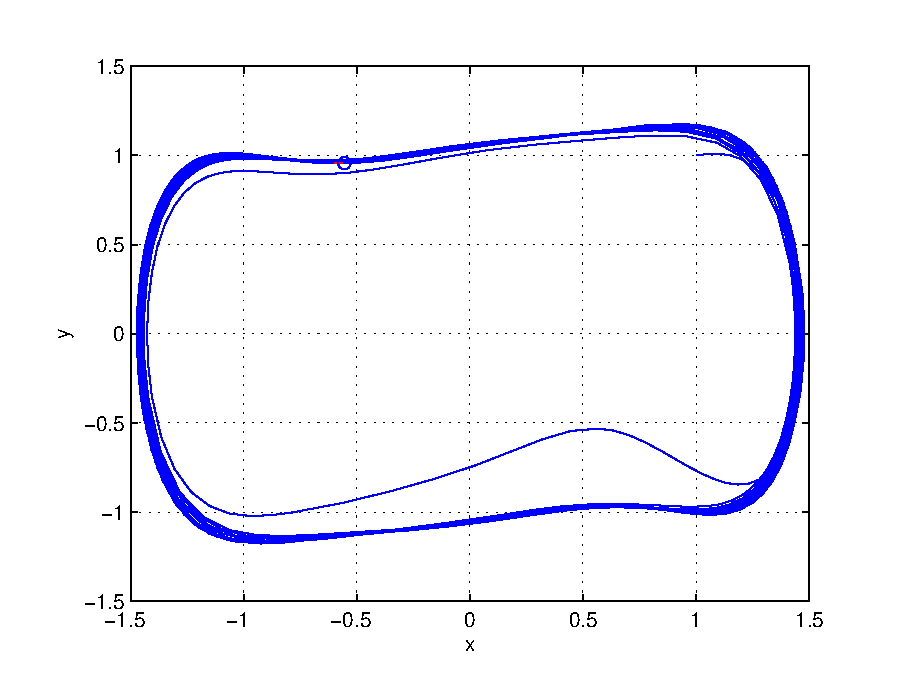
\includegraphics[width=1\linewidth]{duffing_sync.eps}}
	\caption{Фазовый портрет при ${\omega =\omega_{x}}$}
	\label{pic:duffing_sync}
\end{figure}
\begin{figure}[H]
	\center\scalebox{0.5}{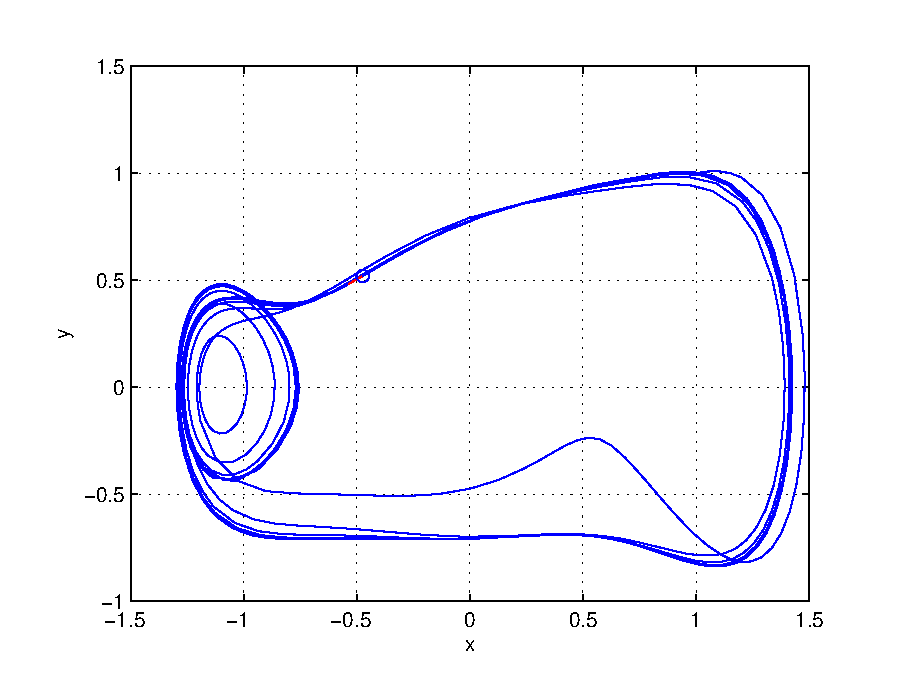
\includegraphics[width=1\linewidth]{duffing_chaos1.eps}}
	\caption{Фазовый портрет при ${\omega < \omega_{x}}$}
	\label{pic:duffing_chaos1}
\end{figure}
\begin{figure}[H]
	\center\scalebox{0.5}{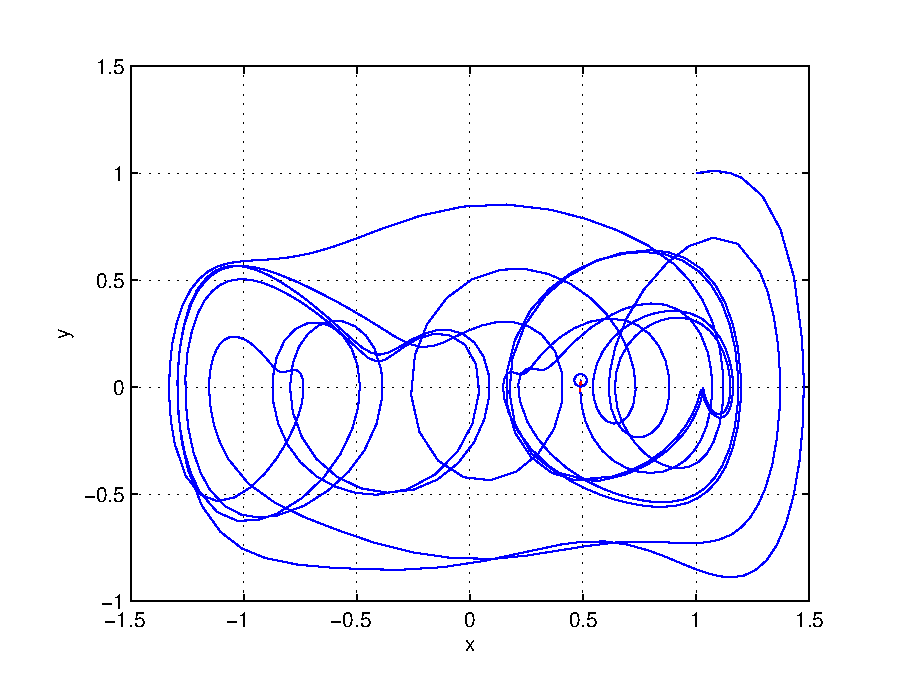
\includegraphics[width=1\linewidth]{duffing_chaos2.eps}}
	\caption{Фазовый портрет при ${\omega > \omega_{x}}$}
	\label{pic:duffing_chaos2}
\end{figure}
В качестве параметров уравнения применялись: $c = 0.5$, $\gamma=\gamma_{x}=0.36$, ${\omega=1}$

Часто для вычисления характеристик хаотической динамики применяется показатель Ляпунова.
Он показывает в каком состоянии находится система. Если система находится
в стабильном состоянии линии фазовой траектории будут близко прилегать одна к другой, в противном
случае система находится в состоянии хаоса. Детектор с применением показателя Ляпунова
представлен на рисунке \ref{pic:chaos_lyapunov}.
\begin{figure}[H]
	\center\scalebox{0.7}{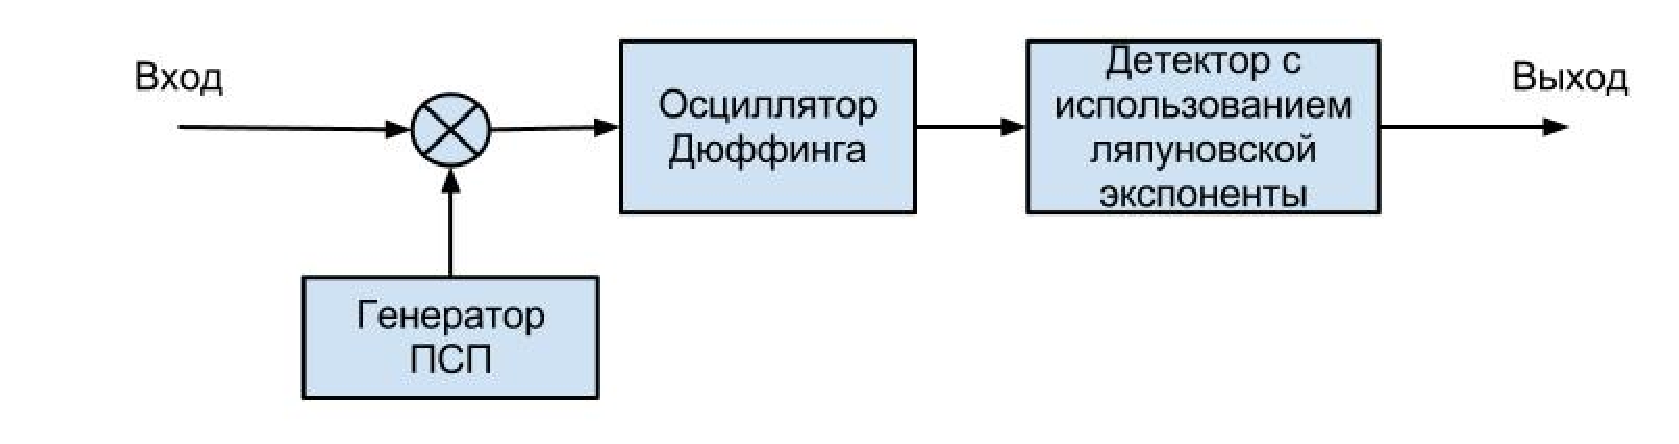
\includegraphics[width=1\linewidth]{Chaos_detector_Lyapunov.eps}}
	\caption{Схема детектора основанного на показателе ляпунова для осциллятора Дуффинга}
	\label{pic:chaos_lyapunov}
\end{figure}

В статье \cite{chaos_chen} предложен усовершенствованный метод, базирующийся на вычислении дисперсии
фазовой траектории. Действительно, на рисунках \ref{pic:duffing_sync}, \ref{pic:duffing_chaos1},
\ref{pic:duffing_chaos2} видно, что когда система находится в хаотическом состоянии значение
дисперсии по координате ${x}$ больше, чем соответствующее значение в состоянии $\omega = \omega_{x}$.
На основе этого была предложена усовершенствованная схема детектора сигнала - рисунок \ref{pic:chaos_energy_detector}
\begin{figure}[H]
	\center\scalebox{0.7}{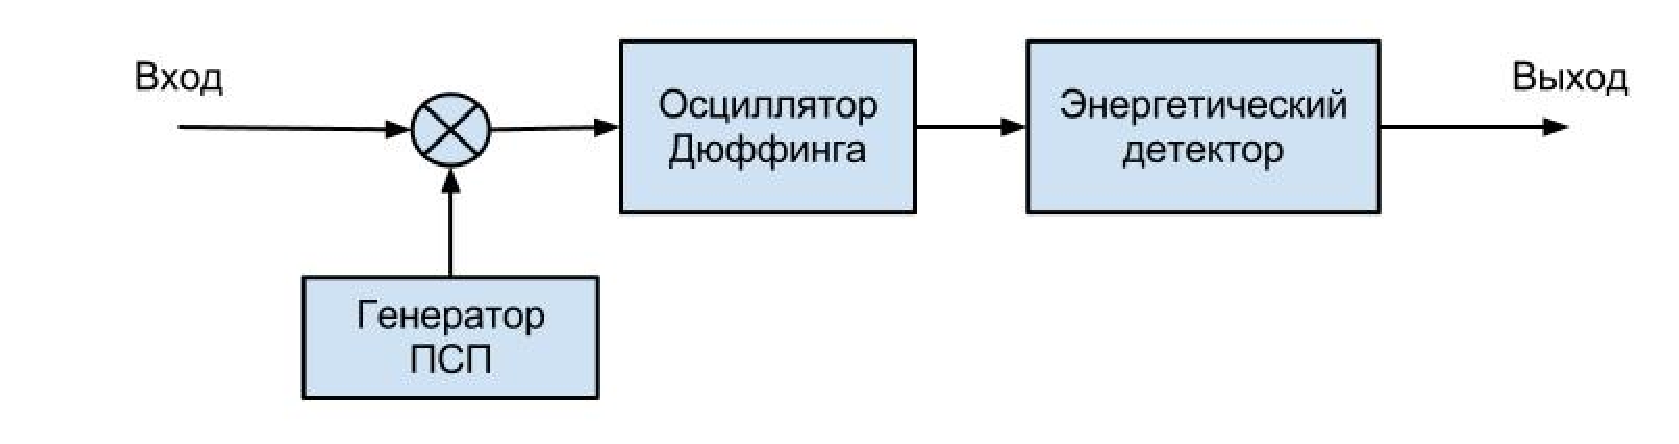
\includegraphics[width=1\linewidth]{chaos_detector.eps}}
	\caption{Схема энергетического детектора для осциллятора Дуффинга}
	\label{pic:chaos_energy_detector}
\end{figure}

%%%%%%%%
% HOS 
Математический аппарат статистик высоких порядков (СВП или HOS - Higher-order statistics)
для исследования непричинных, причинных и нестабильных (систем с неминимальной фазой) и негауссовых сигналов впервые был предложен
в \cite{hos_petropulu} в 1993 году.  Этот метод позволяет не только подавлять цветной Гауссов шум, но так же в некоторых случаях подавлять
цветной не-Гауссов шум.

В работе \cite{hos_zhao} был предложен метод детектирования ШПС с использованием СВП.

%%%%%%%%
% CHE 
Интересная группа алгоритмов основывается на информационной избыточности ШПС, например \cite{phd_che}. В данной
группе алгоритмов используется механизм появления нескольких точек на основном пике КФ, описанный в \cite{kaplan}. Пример
изображен на рисунке \ref{pic:sec1_peak_tcd}.
\begin{figure}[H]
        \center\scalebox{1}{\includegraphics[width=1\linewidth]{corr_peak_tcd.eps}}
        \caption{Идеальная КФ ШПС с отмеченными точками возможного обнаружения}
        \label{pic:sec1_peak_tcd}
\end{figure}
На рисунке \ref{pic:sec1_peak_tcd} изображен пик КФ с несколькими точками. Две точки находятся выше порога ${\Pi=0.5}$.
В работе \cite{phd_che} рассмотрено создание субоптимального обнаружителя на основе информационной избыточности ШПС.
Получена целевая функция системы и намечены дальнейшие пути развития данного направления.

%%%%%%%%
% 2MAX 
Так же одним из направлений исследований является разработка алгоритмов выбора порога без априорной информации о величине ОСШ. Например,
в работах \cite{2max_ieee, 2max_article} представлен алгоритм нахождения пика (АНП) КФ (Peak-finding algorithm).

Данный алгоритм можно разбить на несколько шагов:
\begin{itemize}
\item[Шаг 1] Подсчитать КФ, используя метод предложенный с использованием параллельного коррелятора. 
\item[Шаг 2] Найти главный пик КФ, найти второй пик КФ, найти среднее значение КФ.
\item[Шаг 3] Нормализовать полученные значения относительно главного пика КФ.
\item[Шаг 4] Если (максимум КФ - среднее) > ${\Pi_1}$ и (максимум КФ - 
	второй максимум КФ) > ${\Pi_2}$, тогда полученный главный пик КФ соответствует
	искомой фазе ПСП и частоте.
\end{itemize}

В статье авторов \cite{2max_ieee} предложены следующие значения для порогов:
${\Pi_1} = 0.3$ дБ и  ${\Pi_2} = 0.15$ дБ. Так же авторы предлагают итерационную процедуру для нахождения
фазы ПСП и частоты смещения допплера:
\begin{itemize}
\item[Шаг 1] Начать вычисление с 1мс.
\item[Шаг 2] Получить результаты АНП.
\item[Шаг 3] Если фаза ПСП и частота не могут быть найдены, увеличить время интегрирования сигнала.
	Использовать следующие значения для интегрирования: 1мс -> 10мс -> 50мс -> 100мс -> 200мс ->
	500мс -> 1000мс
\end{itemize}

Очевидным минусом данного подхода является сильная зависимость от интерференции. В городском каньоне будет присутствовать
несколько достаточно мощных лучей, а значит разница в энергии первого и второго пика будет низкой.

%%%%%%
\paragraph{Выводы.}

Во введении кратко приведена история развития СПИ с ШПС, приведены ученые внесшие значительный вклад в разработку данного направления связи. Так же рассмотрена
актуальность исследования в данной области. Кроме того, приведены определения, что такое СПИ с ШПС, ее математическая модель и основные отличительный особенности данного класса систем.
Так же приведены классические и новые подходы к оценке параметров СПИ с ШПС. Рассмотрен оптимальный алгоритм - последовательный коррелятор,
а так же новые достаточно экзотические подходы - применение осциллятора Дуффинга. 

\newpage
 % введение

\addcontentsline{toc}{chapter}{Список сокращений}
\chapter*{Список сокращений}
\noindent
АБГШ - аддитивный белый гауссовский шум				\\
АКП - автокорреляционная последовательность			\\
АКФ – автокорреляционная функция				\\
АНП - алгоритм нахождения пика					\\
АР - авторегрессия						\\
АРСС - авторегрессия скользящего среднего			\\
АЦП - аналогово-цифровой преобразователь			\\
БПФ - быстрое преобразование Фурье				\\
ДПФ - дискретное преобразование Фурье				\\
ДФМ - двоичная фазовая манипуляция				\\
КФ - корреляционная функция					\\
МАВ - максимальная апостериорная вероятность			\\
МНК - метод наименьших квадратов				\\
МШУ - малошумящий усилитель					\\
ОСШ - отношение сигнал-шум 					\\
ПО - программное обеспечение					\\
ПЧ - промежуточная частота					\\
СД - синхронный детектор					\\
СВП - статистики высоких порядков				\\
СНРС - спутниковая навигационная радиоэлектронная система	\\
СНС - спутниковая навигационная система				\\
СКО - средняя квадратическая ошибка				\\
СПМ - спектральная плотность мощности				\\
CC - скользящее среднее						\\
ПСП – псевдослучайная последовательность			\\
УГ - управляемый генератор					\\
ФАП - фазовая автоматическая подстройка				\\
ФАПЧ - фазовая автоподстройка частоты				\\
ФВЧ - фильтр высоких частот					\\
ФНЧ - фильтр низких частот					\\
ФМШПС - фазо-манипупулированный широкополосный сигнал		\\
ЦОС - цифровая обработка сигналов				\\
ШПС -  широкополосные сигналы (шумоподобные сигналы)		\\

\noindent
3G - Third Generation						\\
AGPS - Assisted GPS						\\
BPSK - Binary Phase-Shift Keying				\\
CDMA - Code Division Multiple Access				\\
DAMPS - Digital Advanced Mobile Phone Service			\\
DMA - Delay and Multiply Approach				\\
FTP - file transfer protocol					\\
FPGA - field-programmable gate array 				\\
FPU - floating point unit					\\
GPS - Global Positioning System					\\
GSM - Global System for Mobile Communications (ранее Groupe Spécial Mobile) \\
HOS - Higher-order statistics					\\
NWPR - Narrowband-Wideband Power Ratio				\\
RAM - random access memory					\\
RFID - Radio Frequency IDentification				\\
RSCN - Real Signal-Complex Noise				\\
SDK - Software Development Kit					\\
SDR - Software Defined Receiver					\\
SNV - Signal-to-Noise Variance					\\
SNR - Signal-to-Noise Rate					\\
VHDL - VHSIC ((Very high speed integrated circuits) Hardware Description Language			\\
WAAS - Wide Area Augmentation System				\\


\clearpage
		% acronyms 
\addcontentsline{toc}{section}{СПИСОК УСЛОВНЫХ ОБОЗНАЧЕНИЙ}
\section*{СПИСОК УСЛОВНЫХ ОБОЗНАЧЕНИЙ}
${E[X]}$ - математическое ожидание случайной величины $X$	\\
${D[X]}$ - дисперсия случайной величины $X$			\\
${r_{xx}(\tau)}$ - АКП для смещения ${\tau}$			\\
${\bf{R_M}}$ - автокорреляционная матрица			\\
\newpage
		% definitions

\addcontentsline{toc}{section}{ВВЕДЕНИЕ}
\section*{ВВЕДЕНИЕ}

Большое количество современных систем являются беспроводными. Простота развертывания, мобильность, относительно низкая
стоимость - вот основные преимущества беспроводных систем. Количество мобильных устройств (телефоны, планшетные компьютеры
и т.д.) с каждым годом стремительно растет, только мобильных телефонов в 2011 году было 5.6 миллиарда и покрывало 79.86\%
\cite{wiki_mobilenum} населения земли. Технологии беспроводной связи глубоко проникли во все сферы жизни общества:
обеспечение безопасности с помощью RFID датчиков, предоставление доступа в интернет по технологиями 3G, WiFi, 
сотовая связь по различным технологиям (GSM, CDMA, DAMPS). Некоторые из этих систем строятся на основе методики
расширения спектра, которая отвечает современным требованиям по мощности сигнала, а так же по безопасности передаваемых
данных. В основе таких систем лежат шумоподобные (широкополосные) сигналы - ШПС. Вместе с тем растут требования к таким
системам. Применение ШПС ставит ряд специфических задач по обработке информации, обусловленных особенностями ШПС.
Свойства характерные для ШПС, выгодно отличают данный класс систем от класса узкополосных систем, но с другой стороны
оборачивается усложнением методов обработки ШПС.

Внедрение новых технологий требует увеличение полосы частот. Разнообразие технологий беспроводной передачи данных среди
гражданских и военных систем ведет к перегрузке каналов связи и все более высоким требованиям к скорости передачи
данных. С учётом данных требований применение систем передачи информации с ШПС становится все более востребованным.

Принимая во внимание географические размеры России и стратегическую важность обладания собственными системами спутникового
позиционирования, правительство Российский Федерации уделяет особое внимание разработке собственной системы
глобального спутникового позиционирования ГЛОНАСС. Обладание собственными технологиями системы спутниковой навигации (СНС), государство может обезопасить
себя в случае военных конфликтов от ограничения применения американской системы СНС Navstar GPS в зоне конфликта.

Разработка систем, позволяющих работать с несколькими различными СНС, позволит повысить точность определения координат
в сложных условиях города. Сложность детектирования сигнала и определения координат обусловлена наличием плотной
застройки многоэтажными зданиями. В городских условиях задача подавления интерференционной помехи становится особенно
актуальной. Спектр интерференционной помехи не является белым, а фильтрация и компенсация цветного шума
требует разработки специальных алгоритмов.

Новые цифровые процессоры позволяют применять подходы, которые еще 10-15 лет назад были бесперспективными.
В данной работе развиваются подходы на основе построения параметрической модели ШПС. Невозможность использования
методов требующих вычислений с высокой точностью в приемниках реального времени
10-15 лет назад была обусловлена слабой производительностью процессоров и микроконтроллеров, а так же существенной
стоимостью процессоров с модулем для операций с числами с плавающей точкой. Современное развитие цифровых технологий делает 
возможным применение параметрических методов оценки спектра взамен традиционного подхода основанного на непараметрического
анализа спектра.

Основа теории систем связи с ШПС была заложена в работах В.А. Котельникова и К. Шеннона.
России в этой области занимались В.И. Борисов, В.Б. Пестряков, В.И. Журавлев, М.И. Жодзишский, Б.И. Шахтарин, Л.Е.  Варакин, В.Е. Гантмахер и др.

Изначально методы расширенного спектра применялись при разработке военных систем управления и связи \cite{sklyar}.
К концу второй мировой войны расширение спектра применялось в радиолокации для борьбы с преднамеренными помехами, а
в последствии развитие данной технологии объяснялось желанием создать помехоустойчивые системы связи.
В конце 40-х-начале 50-х годов прошлого века Мортимер Рогофф, сотрудник Международной Телефонной и Телеграфной Корпорации (США) (ITT),
провёл эксперимент по передаче информации при помощи псевдошумового сигнала \cite{sklyar}, среди отечественных ученых
в середине 30-х годов прошлого века работу об основах кодового разделения каналов написал Д.В. Агеев.
Первые разработки таких систем относились к военным отраслям. Данный факт объясняется рядом особенностей, которыми обладают
сигналы с расширенным спектром, в числе которых — сложность перехвата заложенной в них информации,
высокая помехоустойчивость, а также трудность обнаружения факта работы передатчика. В процессе исследований расширенному спектру
нашлось и другое применение - снижение плотности энергии, высокоточная локация, использование при множественном доступе
\cite{sklyar}

Системы связи с широкополосными сигналами занимают особое место. Их особенные свойства выделяют данный класс из других систем
связи. Высокая помехозащищенность при действии сильной помехи, кодовое разделение большого количества абонентов, прием
информации с высокой достоверностью - отличительные особенности широкополосных система. Эти черты были известно, но
уровень элементной базы и низкий уровень помех не позволяли получить развития системам данного класса. Однако развитие
элементной привело к широкому распространению данного вида сигналов. В настоящее они применяются в системах спутниковой навигации,
системах сотовой связи и др \cite{varakin-book}.

Отношение сигнал/шум (ОСШ) на входе приемника может быть очень низким. Для обеспечения высокой помехозащищенности 
в таких случаях используются ШПС с большими и сверхбольшими базами.

К созданию сложных широкополосных сигналов (СШС) привело решение ряда проблем при развитии систем передачи данных.
Первая проблема встала при разработке новых радиолокационных система. Для дальнейшего развития требовалось
решить несколько противоречий: требование высокой разрешающей способности по дальности и дальностью обнаружения
целей в импульсных РЛС, требование точного измерения скорости и высокое разрешение по дальности, требование
увеличить дальность при ограничении пиковой мощности \cite{gantmaher-book}. Решение данных задач было предложено
Ф. Вудвардом. Им было показано, что дополнительным параметром является форма сигнала. Длительность сигнала
может быть больше - настолько больше, насколько это необходимо для обеспечения энергетических требований, а требование
разрешения по дальности и точности измерений определяются шириной полосы сигнала. Данные требования обеспечивается
путем сжатия импульса на стороне приемника. Вудворд сформулировал принципы: произведение эффективной полосы частот
радиосигнала на его длительность должен быть существенно больше единиц ${FT>>1}$, внутренняя структура сигнала
должна быть такой, чтобы обеспечить возможность приемнику сжатие распределенного во времени сигнала в короткий импульс,
соответствующий полосе ${F}$ \cite{gantmaher-book}.

В \cite{gantmaher-book} показана связь пропускной способности канала с понятием ШПС. При ${R_e<<1}$ можно записать:
\begin{center}
\begin{equation}
	\label{eq:shennon_cdma}
	FT = \frac{1}{\log(1+R_e)},
\end{equation}
\end{center}
где ${R_e}$ - ОСШ, ${F}$ - эффективная полоса частот, ${T}$ - длительность.

Стоить отметить, что при ${R_e<<1}$, левая часть выражения \ref{eq:shennon_cdma} стремится к бесконечности, а значит
ШПС позволяет обеспечить теоретически неограниченную достоверность передачи информации. Второе важное свойство
ШПС, следующее из \ref{eq:shennon_cdma} - способность работать "под шумами". Что обеспечивает скрытность
передачи информации, а с другой высокую степень уплотнения каналов связи и, как следствие, решение современных проблем
с перегруженностью каналов связи.

В данной работе будет рассматриваться ШПС модулированный ПСП на основе двоичной рекуррентной последовательности.
Для выделения данных из потока необходимо иметь точно синхронизированную копию ПСП, которая была использована
при модулировании сигнала на передающей стороне. Для достижения синхронизма на стороне приемника необходимо
устранить неопределенность в двух областях: неопределенность по частоте и неопределенность по фазе (задержке) ПСП.
Неопределенность по фазе ПСП обусловлена неопределенностью в расстоянии между передатчиком и приемником. Неопределенность
по частоте обусловлена в первую очередь допплеровским эффектом, а так же нестабильностью опорных генераторов в
передатчике и приемнике. После устранения неопределенности по частоте для достижения точной синхронизации
начинается процесс слежения за частотой. Неопределенность по фазе ПСП устранить, не используя полный перебор,
невозможно в силу корреляционных свойств ПСП. Таким образом можно заключить, что задача быстрого и эффективного
поиска и оценки параметров ШПС является актуальной.

В данной работе рассматривается подход программного приемника (Software Defined Receiver - SDR)
\cite{akos-book, grayver-book, pany-book} для оценки параметров ШПС. Как уже было отражено выше, ШПС применяется во
многих системах. В данной работе для полунатурного эксперимента будет рассматриваться сигнал СНС Navstar GPS. Данная система передачи 
информации использует ПСП Голда \cite{gold-ieee} для модулирования сигнала.

Традиционные подходы к реализации приемника СНС Navstar GPS отражены в \cite{akos-book, tsui}. 

Популярность и распространенность данной системы стимулирует исследования в области детектирования
и оценки частоты ШПС сигналов.

Существуют исследования в области применения теории хаоса - детектирование и оценка
частоты ШПС с применением осциллятора Дуффинга \cite{chaos_cambridge, chaos_chen, chaos_huang, chaos_wang}. Преимуществом
данного подхода является то, что свойства осциллятора позволяют детектировать сигналы с экстремально низким ОСШ. В то же
время, на данный момент никто не предложил цифровое представление осциллятора Дуффинга, а это затрудняет использование данного подхода
в реальных приемниках. Таким образом данное направление является в настоящее время больше теоретическим, чем практическим.

В работах \cite{hos_petropulu, hos_zhao} предложено использовать статистики высоких порядков для подавления шума и детектирование
сигналов с низким уровнем ОСШ.

Более традиционные подходы для детектирования и оценки параметров ШПС сигналов с низким уровнем ОСШ рассмотрены в монографии \cite{ziedan-book}.
В данной монографии рассматриваются как методы детектирования и оценки параметров ШПС, основанные на когерентном накоплении, так и эффективные
системы слежения за частотой и фазой ПСП.

{\bf{Добавить ЦЕЛИ И ЗАДАЧИ}}

%%%%%%
\paragraph{Постановка задачи оценки параметров сигнала с расширенным спектром.}
В данной работе рассматриваются задачи повышения рабочих характеристик приемников ШПС, поэтому целесообразно отразить основные модули этой системы 
на примере СНС Navstar GPS - рисунок \ref{pic:sec1_gnss_system}.
\begin{figure}[H]
\center\scalebox{1}{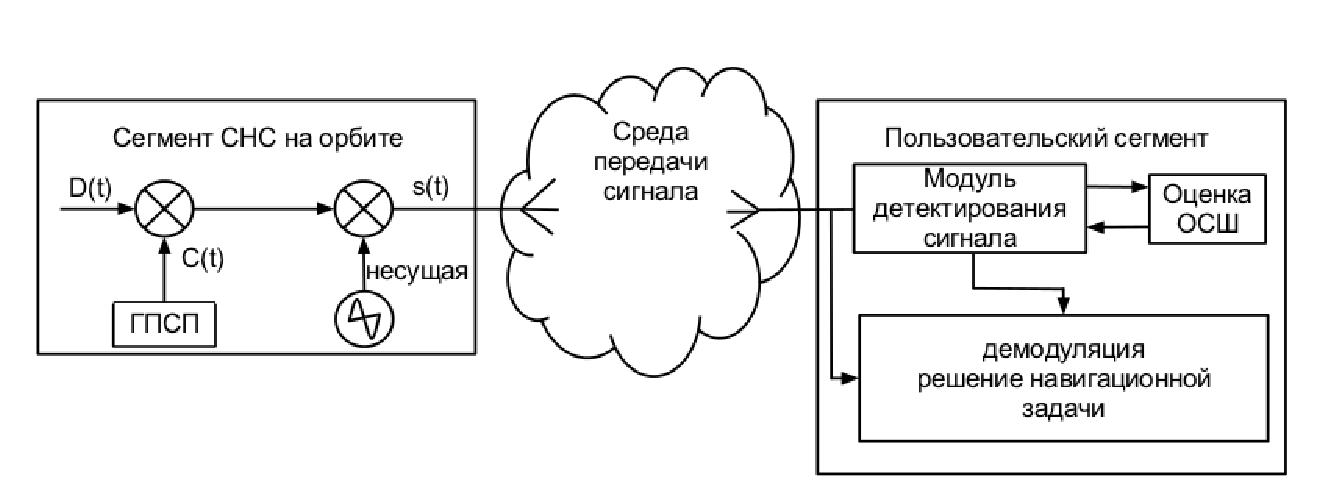
\includegraphics[width=1\linewidth]{sec1gnss_system.eps}}
\caption{структутраная схема СНС GPS}
\label{pic:sec1_gnss_system}
\end{figure}

В систему СНС Navstar GPS входят космический сегмент, наземный сегмент (на рисунке \ref{pic:sec1_gnss_system} не
отражен), а так же пользовательский сегмент. В космический сегмент входит спутниковая группировка, в 
наземный - станции управления, в пользовательский - все устройства принимающие сигнал от СНС GPS.

\paragraph{Модель сигнала и помех.}
В системе СНС Navstar GPS применяется ШПС.
Система передачи информации считается системой с расширенным спектром в следующих случаях \cite{sklyar}:
\begin{enumerate}
	\item Используемая полоса значительно шире минимальной, необходимой для передачи данных.
	\item Расширение спектра производится с помощью так называемого расширяющего сигнала (ПСП),
		который не зависит от передаваемой информации.
	\item Восстановление исходных данных ("сужение спектра") осуществляется путем сопоставления полученного
		сигнала и синхронизированной копии расширяющего сигнала (ПСП)
\end{enumerate}

Так же подобные сигналы называют:
\textquotedblleftсложными\textquotedblright,
\textquotedblleftшумоподобными\textquotedblright,
\textquotedblleftпсевдослучайными\textquotedblright,
\textquotedblleftсложными-дискретными\textquotedblright,
\textquotedblleftдискретно-кодированными\textquotedblright,
\textquotedblleftортогональными (квазиортогональными)\textquotedblright,
\textquotedblleftоптимальными дискретными\textquotedblright
\cite{gantmaher-book}.

Каждое название ставит акцент на определенной характеристике сигнала. В данной работе я буду оперировать термином
широкополосный сигнал - ШПС. ШПС можно определить как \cite{gantmaher-book, varakin-book}:
\begin{center}
\begin{equation}
	\label{eq:ss_signal}
	1 << FT = B,
\end{equation}
\end{center}
где: ${B}$ - база сигнала, ${F}$ - эффективная ширина спектра, а ${T}$ - длительность.
Неточность этого определения рассмотрена в \cite{gantmaher-book}, так же там даны ссылки на другие источники
разделяющие критику данного определения. Для данной работы критика, рассмотренная в приведенных источниках,
принципиального значения не имеет.

%%%%%%
\paragraph{Классическая постановка задачи оценки параметра.}
Из литературы по теории автоматических систем, например \cite{pugachev} (глава 10.1), известна классическая постановка
задачи задачи теории оптимальных систем. "На практике часто приходится решать задачу проектирования системы, когда
требуется определить характеристики системы таким образом, чтобы она имела наибольшую точность при данных условиях.
Систему обеспечивающую наибольшую возможную точность с какой-нибудь определенной точки зрения среди всех систем
заданного класса, обычно называют оптимальной" \cite{pugachev}.

В одной из постановок данной задачи \cite{pugachev} (глава 10.1), система считается полностью неизвестной
и требуется определить ее оператор так, чтобы она была оптимальной с точки зрения принятого критерия качества. Эта
задача сводится к определению с наибольшей возможной точностью некоторых параметров, от которых зависит принимаемый
сигнал. Но при этом важно учитывать не только точность, но и другие факторы, так как проектируемая система должна
удовлетворять многим, часто противоречивым требованиям. В виду приведенных факторов, обычно представляет собой
ряд компромиссных решений, удовлетворяющих всем предъявляемым к системе требованиям.

Точность автоматической системы обычно характеризуется математическим ожиданием и дисперсией ее ошибки.
Математическое ожидание представляет собой систематическую ошибку системы в данных условиях, а дисперсия
характеризует уровень случайных ошибок \cite{pugachev} (глава 10.2). Так как в различных условиях работы
системы, которые встречаются случайно систематическая ошибка тоже является случайной, за критерий качества
системы при ее проектировании обычно принимают второй начальный момент ошибки - математическое ожидание
квадрата ошибки:
\begin{center}
\begin{equation}
	\label{eq:stat_err_prob}
	\eta = M[e^2(t)]
\end{equation}
\end{center}
Положительный квадратный корень из этой величины называют средней квадратичной ошибкой системы. Таким образом,
оптимальной системой обычно считают такую систему, которая имеет минимальную среднюю квадратичную ошибку.

Критерий минимума средней квадратичной ошибки является простейшим с математической точки зрения и обычно приводит
к наиболее простым методам определения оптимальных систем. Однако далеко не во всех задачах он может служить мерой
качества системы. Поэтому нельзя ограничиваться методами нахождения оптимальных систем по критерию минимума средней
квадратичной ошибки.

В случаях, когда необходимо проектировать следящую систему, приходится учитывать возможность срыва слежения,
который заключается в том что система перестает работать, если ее ошибка превосходит по абсолютной величине некоторый
уровень. При проектировании таких систем целесообразно принять за критерий качества вероятность срыва слежения. При
этом оптимальной считается такая система, которая обеспечивает минимум вероятности срыва слежения. Если срыв слежения
происходит в случае, когда абсолютная величина ошибки превосходит уровень $a$, то критерий минимума вероятности ошибки
слежения можно представить \cite{pugachev} (глава 10.2):
\begin{center}
\begin{equation}
	\label{eq:prob_lost_signal}
	p = P(e(t) > a) = min
\end{equation}
\end{center}

%%%%%%
\paragraph{Введение обозначений.}
В диссертации рассматривается сигнал с расширенным спектром полученный методом "прямой последовательности".
Данный метод заключается в том, что гармоническая несущая сигнала модулируется высокоскоростным (широкополосным)
расширяющим сигналом (ПСП). 

Несущее колебание с частотой ${\omega_0}$  модулируется данными ${d(t)}$ , а также высокоскоростной ПСП ${g(t)}$, полученной методом "прямой последовательности".
СПИ Navstar GPS осуществляется двоичная фазовая модуляция (ДФМ или 2-ФМ), а значит ${d(t)}$  и ${g(t)}$  - потоки антиподных импульсов \{-1, 1\}.
Таким образом сигнал на выходе модулятора может быть представлен \cite{shahtarin_sync}:
\begin{equation}
	\label{eq:cdma_eq}
	s(t)=Ad(t)g(t)\cos{(\omega_{0}t)},
\end{equation}
где ${d(t)}$- информационный бит, а ${g(t)}$ - ПСП представляет собой фазовый сдвиг  ${0, \pi}$.

В реальных СПИ сигнал на приемник поступает одновременно от нескольких источников, присутствует неопределенность по частоте, а также аддитивный белый шум (АБГШ).
В приемнике после оцифровки сигнала получаем смесь:
\begin{equation}
	\label{eq:cdma_strip_eq}
	x(m)=\sum_{k=1}^{N}\left( A_k g(m + \tau_k)\exp{\left[j \left( \tilde{\omega}_{k}m + \phi_k(m)\right)\right]} \right) + n(m),
\end{equation}
где  ${k}$ - относительный номер источника сигнала, ${N}$ - количество доступных источников сигнала, модулированных ПСП одного семейства,
${m}$ - индекс соответствующий времени, ${\tilde{\omega}_{k}}$  – относительная частота, соответствующая ${\omega_0}$,
${\tau_k}$ - задержка модулирующей ПСП в точке приема, ${\phi_k(m)}$ - случайная начальная фаза, ${n(m)}$ - аддитивный белый гауссов шум (АБГШ). 

Следует отметить, что при оценке фазы сигнала с номером ${k}$  интерференцией являются сигналы:    .
\begin{equation}
	%\label{eq:cdma_interference}
	\{n \ne k, n \in [1,N]\}
\end{equation}

%%%%%%
\paragraph{Алгоритмы оценки параметров широкополосного сигнала сигнала.}
Алгоритм реализующий метод максимального правдоподобия - последовательный коррелятор. Данный подход реализуется в аппаратных приемниках.
Аппаратный приемник позволяет реализовать параллельно несколько последовательных корреляторов и вести оценку параметров
СПИ с ШПС параллельно.

Данный алгоритм в некоторых источниках так же называется согласованным фильтром. В \cite{sklyar} рассмотрены нюансы этих двух понятий.
В данной работе используется понятие последовательный коррелятор. Работа коррелятора описывается математической операцией
корреляции \ref{eq:serial_corr}. Сигнал коррелируется с локальной копией и на выходе коррелятора получается значение, отражающее
степень совпадения сигналов. Не трудно представить, что сигнал с хорошими корреляционными свойствами должен обладать высоким значением
корреляции когда сигналы синхронизированы и минимальным значением в любом другом случае (фаза ПСП не выровнена - отсутствие сигнала).
\begin{equation}
	\label{eq:serial_corr}
	y(n)=\sum\limits_{m=0}^{N-1}{x(m)h(n+m)},
\end{equation}
где ${x(m)}$ - принятая смесь, а ${h(n)}$ не импульсная характеристика системы, а локальная копия сигнала.

%%%%%%%%
% DFT

Вычисление циклической свертки через дискретное преобразование Фурье (ДПФ) - достаточно популярный метод
в программных приемниках, так как позволяет существенно уменьшить количество операций при вычислении. Но, как показано
в \cite{tsui, oppenheim}, можно достаточно просто перейти от свертки к циклической корреляции. Так как этот метод является самым
популярным в программных приемниках стоит его представить.
Свертка может быть представлена как:
\begin{equation}
	\label{eq:fft_conv}
	y(n)=\sum\limits_{m=0}^{N-1}{x(m)h(n-m)}
\end{equation}

Стоит отметить, что в \ref{eq:fft_conv} сдвиг во времени является циклическим, поскольку дискретные операции являются циклическими.
Возьмем ДПФ от \ref{eq:fft_conv}
\begin{center}
\begin{eqnarray}
	\label{eq:fft_conv_fft}
	Y(k) & = & \sum\limits_{n=0}^{N-1}\sum\limits_{m=0}^{N-1}{x(m)h(n-m)e^{(-j2\pi{kn})/N}}=\nonumber \\
	& = & \sum\limits_{m=0}^{N-1}{x(m)}[\sum\limits_{n=0}^{N-1}h(n-m)e^{(-j2\pi{(n-m)}k)/N}]e^{(-j2\pi{m}k)/N}=\\
	& = & H(k)\sum\limits_{m=0}^{N-1}e^{(-j2\pi{m}k)/N} = X(k)H(k)\nonumber 
\end{eqnarray}
\end{center}
Из уравнения \ref{eq:fft_conv_fft} легко видеть, что это не линейная свертка. В линейной свертке для входного сигнала размером в ${N}$ точек,
результат будет из ${2N-1}$ точек. А в уравнении выше, результатом является всего ${N}$ точек.
Это проявление циклической природы ДПФ.

Алгоритм оценки не использует свертку, он использует корреляцию, которая отличается от свертки. Корреляция
между $x(n)$ и $h(n)$ записывается выражением \ref{eq:serial_corr}:
Единственным отличаем между \ref{eq:serial_corr} и \ref{eq:fft_conv} является знак перед $m$ в ${h(n+m)}$.
В случае оценки параметра ШПС, $h(n)$ является локальной копией сигнала, а не импульсной характеристикой.
Произведем ДПФ над $z(n)$:
\begin{center}
\begin{eqnarray}
	\label{eq:fft_corr_fft}
	Z(k) & = & \sum\limits_{n=0}^{N-1}\sum\limits_{m=0}^{N-1}{x(m)h(n+m)e^{(-j2\pi{kn})/N}}=\nonumber \\
	& = & \sum\limits_{m=0}^{N-1}{x(m)}[\sum\limits_{n=0}^{N-1}h(n+m)e^{(-j2\pi{(n+m)}k)/N}]e^{(j2\pi{m}k)/N}=\\
	& = & H(k)\sum\limits_{m=0}^{N-1}e^{(j2\pi{m}k)/N} = X(k)H^{-1}(k)\nonumber 
\end{eqnarray}
\end{center}
где ${X^{-1}(k)}$ - обратное ДПФ. Уравнение \ref{eq:fft_corr_fft} можно записать как:

\begin{equation}
	\label{eq:fft_corr_fft_rev}
	Y(k) = \sum\limits_{n=0}^{N-1}\sum\limits_{m=0}^{N-1}{x(n+m)h(m)e^{(-j2\pi{kn})/N}}=X^{-1}(k)H(k)
\end{equation}

Если сигнал $x(n)$ действительный, то $x(n) = x^*(n)$, где ${^*}$ - операция комплексного сопряжения. Используя данное соотношение,
значение $Z(k)$ может быть записано:
\begin{equation}
	\label{eq:fft_magnitude}
	|Z(k)|=|H^*(k)X(k)|=|H(k)X(k)^*|
\end{equation}
Данное соотношение может быть использовано для нахождения значения циклической корреляции между входным сигналом и 
локальной копией.

%%%%%%%%
% Chaos 
Оценка параметров СПИ с ШПС (в частности сигналов системы Navstar GPS) с помощью осциллятора Дуффинга
достаточно новое направление в исследованиях по данной тематике. В данной области опубликовано несколько работ, в частности \cite{chaos_chen, chaos_cambridge, chaos_huang, chaos_song}.
Так же является интересной более ранняя статья не рассматривающая GPS \cite{chaos_wang}.
Осциллятор Дуффинга с гармоническим внешним воздействием может быть описан уравнением:
\begin{center}
\begin{equation}
	\label{eq:duffing}
	mx'' + cx' + k_{1}x + k_{2}x^3 = F_{0}\cos(\omega{t}),
\end{equation}
\end{center}
где $m$ - масса, $c$ - коэффициент диссипации, $x$ - состояние осциллятора, $k_1$ и $k_2$ - линейный и нелинейный коэффициенты соответственно,
$F_{0}\cos(\omega{t})$ - внешнее воздействие.

Подробно уравнение \ref{eq:duffing} рассмотрено в \cite{chaos_neimark_landa}.
Для использования осциллятора Дуффинга с целью оценки параметров ШПС была предложена усовершенствованная форма \cite{chaos_song, chaos_chen}:
\begin{center}
\begin{equation}
	\label{eq:duffing_gps}
	x'' +cx' - x^3 + x^5 = \gamma\cos(\omega{t}) + (\gamma_{x}\cos(\omega_{x}) + n(t))
\end{equation}
\end{center}

Перепишем динамическую систему \ref{eq:duffing_gps} в виде:
\begin{center}
\begin{equation}
	\label{eq:duffing_gps_2}
	\left\{
	\begin{aligned}
		y(t) & = x'(t) \\
		y'(t) & =  -cx' + x^3 - x^5 + \gamma\cos(\omega{t}) + (\gamma_{x}\cos(\omega_{x}) + n(t)),
	\end{aligned}
	\right.
\end{equation}
\end{center}
где ${n(t)}$ - АБГШ.

Пример фазового портрета при ${\omega=\omega_{x}}$ изображен на рисунке \ref{pic:duffing_sync},
фазовый портрет хаоса расположен на рисунках \ref{pic:duffing_chaos1}, \ref{pic:duffing_chaos2}
\begin{figure}[H]
	\center\scalebox{0.5}{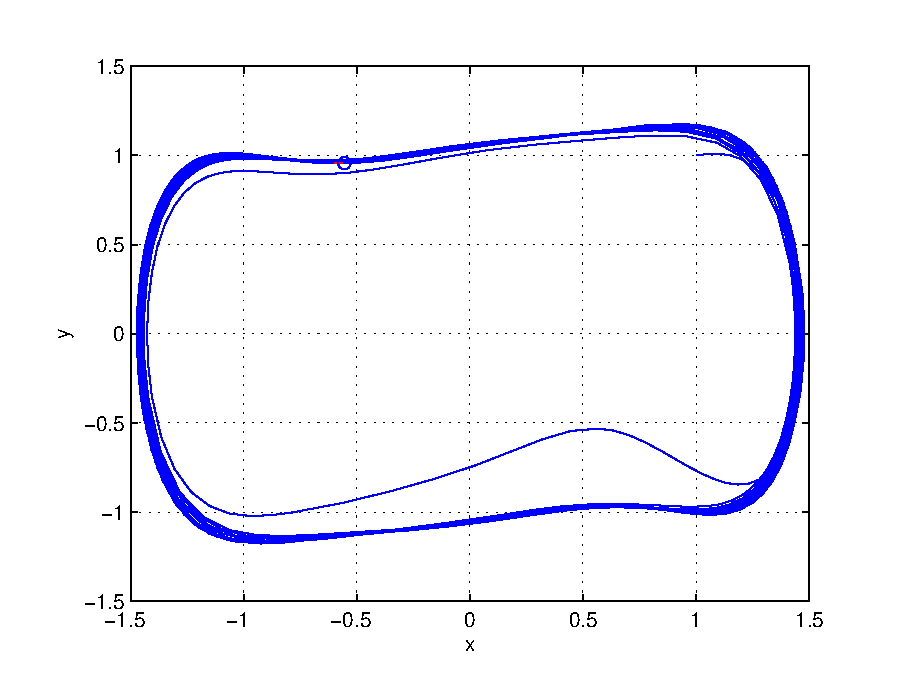
\includegraphics[width=1\linewidth]{duffing_sync.eps}}
	\caption{Фазовый портрет при ${\omega =\omega_{x}}$}
	\label{pic:duffing_sync}
\end{figure}
\begin{figure}[H]
	\center\scalebox{0.5}{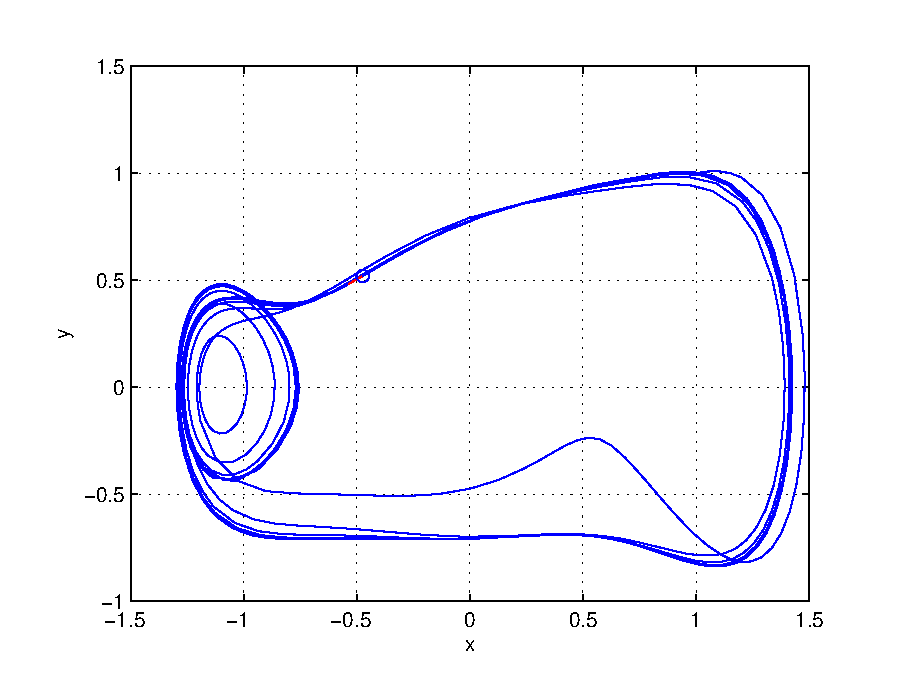
\includegraphics[width=1\linewidth]{duffing_chaos1.eps}}
	\caption{Фазовый портрет при ${\omega < \omega_{x}}$}
	\label{pic:duffing_chaos1}
\end{figure}
\begin{figure}[H]
	\center\scalebox{0.5}{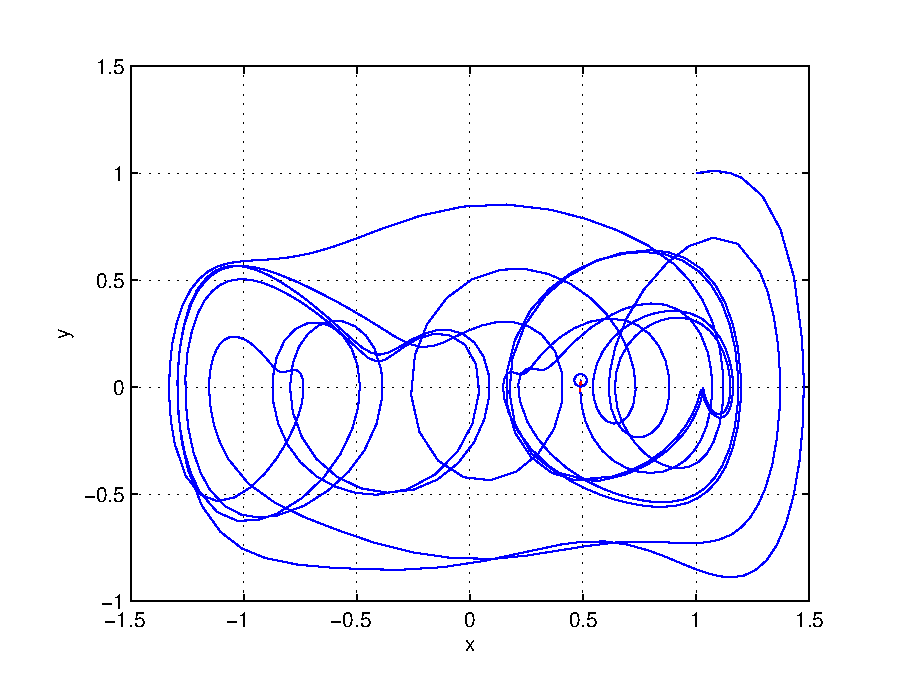
\includegraphics[width=1\linewidth]{duffing_chaos2.eps}}
	\caption{Фазовый портрет при ${\omega > \omega_{x}}$}
	\label{pic:duffing_chaos2}
\end{figure}
В качестве параметров уравнения применялись: $c = 0.5$, $\gamma=\gamma_{x}=0.36$, ${\omega=1}$

Часто для вычисления характеристик хаотической динамики применяется показатель Ляпунова.
Он показывает в каком состоянии находится система. Если система находится
в стабильном состоянии линии фазовой траектории будут близко прилегать одна к другой, в противном
случае система находится в состоянии хаоса. Детектор с применением показателя Ляпунова
представлен на рисунке \ref{pic:chaos_lyapunov}.
\begin{figure}[H]
	\center\scalebox{0.7}{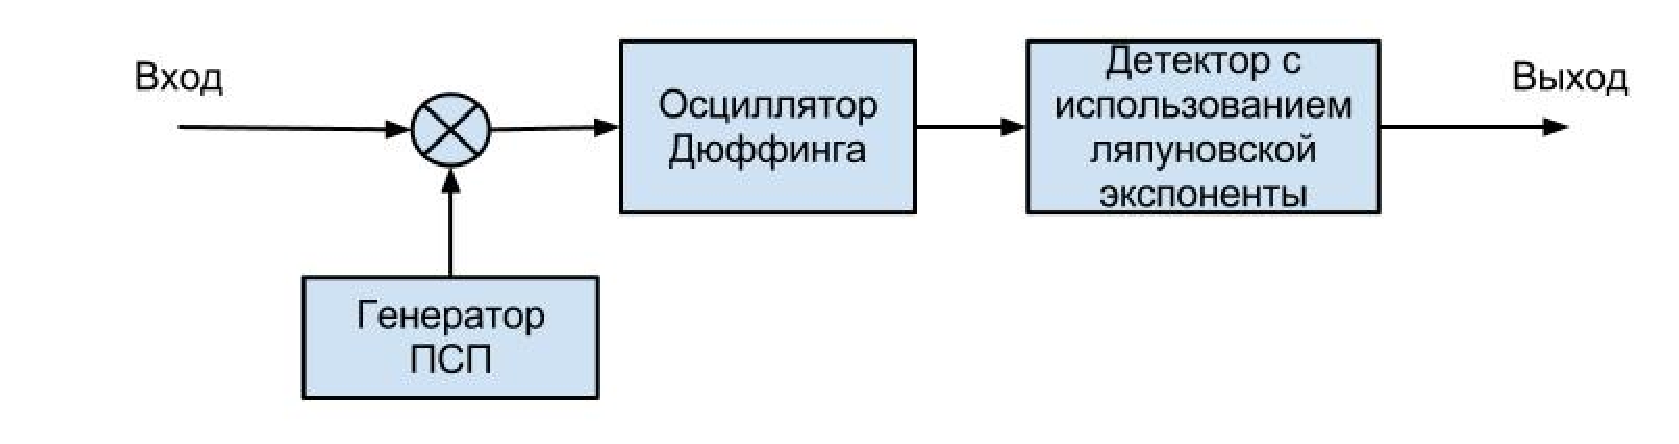
\includegraphics[width=1\linewidth]{Chaos_detector_Lyapunov.eps}}
	\caption{Схема детектора основанного на показателе ляпунова для осциллятора Дуффинга}
	\label{pic:chaos_lyapunov}
\end{figure}

В статье \cite{chaos_chen} предложен усовершенствованный метод, базирующийся на вычислении дисперсии
фазовой траектории. Действительно, на рисунках \ref{pic:duffing_sync}, \ref{pic:duffing_chaos1},
\ref{pic:duffing_chaos2} видно, что когда система находится в хаотическом состоянии значение
дисперсии по координате ${x}$ больше, чем соответствующее значение в состоянии $\omega = \omega_{x}$.
На основе этого была предложена усовершенствованная схема детектора сигнала - рисунок \ref{pic:chaos_energy_detector}
\begin{figure}[H]
	\center\scalebox{0.7}{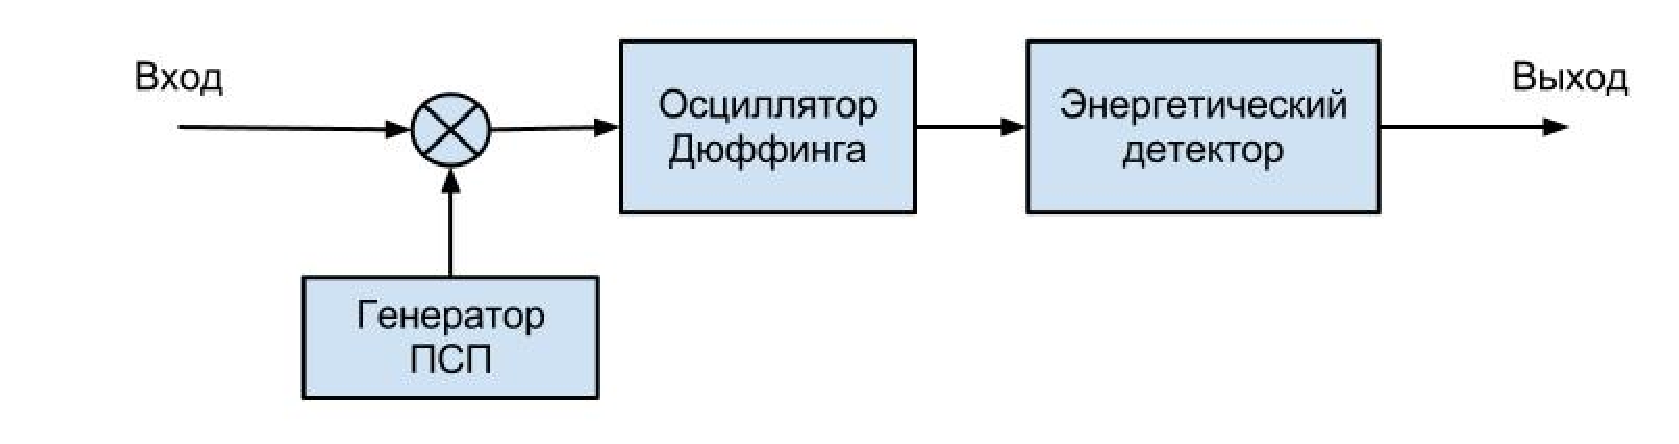
\includegraphics[width=1\linewidth]{chaos_detector.eps}}
	\caption{Схема энергетического детектора для осциллятора Дуффинга}
	\label{pic:chaos_energy_detector}
\end{figure}

%%%%%%%%
% HOS 
Математический аппарат статистик высоких порядков (СВП или HOS - Higher-order statistics)
для исследования непричинных, причинных и нестабильных (систем с неминимальной фазой) и негауссовых сигналов впервые был предложен
в \cite{hos_petropulu} в 1993 году.  Этот метод позволяет не только подавлять цветной Гауссов шум, но так же в некоторых случаях подавлять
цветной не-Гауссов шум.

В работе \cite{hos_zhao} был предложен метод детектирования ШПС с использованием СВП.

%%%%%%%%
% CHE 
Интересная группа алгоритмов основывается на информационной избыточности ШПС, например \cite{phd_che}. В данной
группе алгоритмов используется механизм появления нескольких точек на основном пике КФ, описанный в \cite{kaplan}. Пример
изображен на рисунке \ref{pic:sec1_peak_tcd}.
\begin{figure}[H]
        \center\scalebox{1}{\includegraphics[width=1\linewidth]{corr_peak_tcd.eps}}
        \caption{Идеальная КФ ШПС с отмеченными точками возможного обнаружения}
        \label{pic:sec1_peak_tcd}
\end{figure}
На рисунке \ref{pic:sec1_peak_tcd} изображен пик КФ с несколькими точками. Две точки находятся выше порога ${\Pi=0.5}$.
В работе \cite{phd_che} рассмотрено создание субоптимального обнаружителя на основе информационной избыточности ШПС.
Получена целевая функция системы и намечены дальнейшие пути развития данного направления.

%%%%%%%%
% 2MAX 
Так же одним из направлений исследований является разработка алгоритмов выбора порога без априорной информации о величине ОСШ. Например,
в работах \cite{2max_ieee, 2max_article} представлен алгоритм нахождения пика (АНП) КФ (Peak-finding algorithm).

Данный алгоритм можно разбить на несколько шагов:
\begin{itemize}
\item[Шаг 1] Подсчитать КФ, используя метод предложенный с использованием параллельного коррелятора. 
\item[Шаг 2] Найти главный пик КФ, найти второй пик КФ, найти среднее значение КФ.
\item[Шаг 3] Нормализовать полученные значения относительно главного пика КФ.
\item[Шаг 4] Если (максимум КФ - среднее) > ${\Pi_1}$ и (максимум КФ - 
	второй максимум КФ) > ${\Pi_2}$, тогда полученный главный пик КФ соответствует
	искомой фазе ПСП и частоте.
\end{itemize}

В статье авторов \cite{2max_ieee} предложены следующие значения для порогов:
${\Pi_1} = 0.3$ дБ и  ${\Pi_2} = 0.15$ дБ. Так же авторы предлагают итерационную процедуру для нахождения
фазы ПСП и частоты смещения допплера:
\begin{itemize}
\item[Шаг 1] Начать вычисление с 1мс.
\item[Шаг 2] Получить результаты АНП.
\item[Шаг 3] Если фаза ПСП и частота не могут быть найдены, увеличить время интегрирования сигнала.
	Использовать следующие значения для интегрирования: 1мс -> 10мс -> 50мс -> 100мс -> 200мс ->
	500мс -> 1000мс
\end{itemize}

Очевидным минусом данного подхода является сильная зависимость от интерференции. В городском каньоне будет присутствовать
несколько достаточно мощных лучей, а значит разница в энергии первого и второго пика будет низкой.

%%%%%%
\paragraph{Выводы.}

Во введении кратко приведена история развития СПИ с ШПС, приведены ученые внесшие значительный вклад в разработку данного направления связи. Так же рассмотрена
актуальность исследования в данной области. Кроме того, приведены определения, что такое СПИ с ШПС, ее математическая модель и основные отличительный особенности данного класса систем.
Так же приведены классические и новые подходы к оценке параметров СПИ с ШПС. Рассмотрен оптимальный алгоритм - последовательный коррелятор,
а так же новые достаточно экзотические подходы - применение осциллятора Дуффинга. 

\newpage


\setcounter{chapter}{1}
\setcounter{section}{0}
\setcounter{equation}{0}
\setcounter{figure}{0}
\addcontentsline{toc}{chapter}{Глава 1. Алгоритм оценки информационных параметров для одного источника сигнала в CDMA-системах на фоне АБГШ}
\chapter*{Глава 1. Алгоритм оценки информационных параметров для одного источника сигнала в CDMA-системах на фоне АБГШ}

\section{Постановка задачи}
В данной главе ставится и решается задача синтеза  
алгоритма оценки информационных параметров ШПС на основе авторегрессионной модели сигнала для одного источника на фоне АБГШ,
также рассмотрены источники помех и оптимальный в смысле максимального правдоподобия приемник для CDMA-системы Navstar GPS. 
Точность оценки приведенного алгоритма сравнивается с границей Крамера-Рао. 

Объектом исследования являются приемники типового широкополосного сигнала - СНС Navstar GPS.
Сигнал данной системы был выбран по причине относительно простой возможности к его доступу (сбору сигнала, а также наличию уже собранного сигнала в общедоступных источниках) и широкого распространения.
Основные модули этой системы изображены на \mbox{Рис. \ref{pic:sec1_gnss_system}.}
\begin{figure}[h]
	\center\scalebox{1}{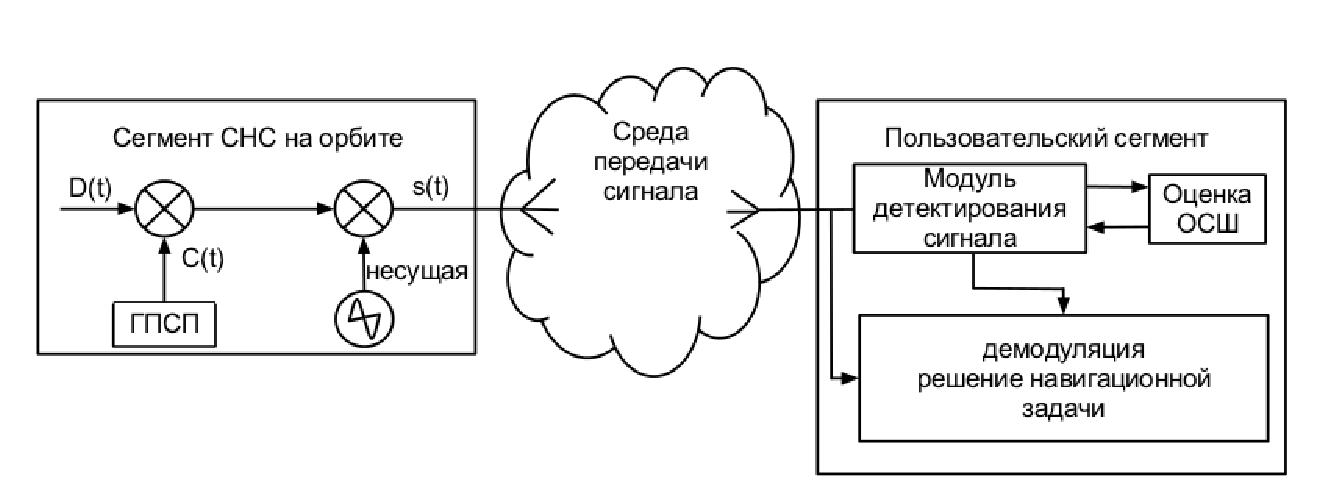
\includegraphics[width=1\linewidth]{sec1gnss_system.eps}}
	\caption{Структурная схема СНС GPS}
	\label{pic:sec1_gnss_system}
\end{figure}
В систему СНС Navstar GPS входят космический сегмент, наземный сегмент (на Рис. \ref{pic:sec1_gnss_system} не
отражен), а также пользовательский сегмент. В космический сегмент входит спутниковая группировка, в 
наземный - станции управления, в пользовательский - все устройства, принимающие сигнал от СНС Navstar GPS.

%В системе СНС Navstar GPS применяется ШПС. Система передачи информации считается системой с расширенным спектром в следующих случаях \cite{sklyar}:
%\begin{enumerate}
%	\item Используемая полоса значительно шире минимальной, необходимой для передачи данных.
%	\item Расширение спектра производится с помощью так называемого расширяющего сигнала (ПСП),
%		который не зависит от передаваемой информации.
%	\item Восстановление исходных данных ("сужение спектра") осуществляется путем сопоставления полученного
%		сигнала и синхронизированной копии расширяющего сигнала (ПСП)
%\end{enumerate}
%
%Так же подобные сигналы называют:
%\textquotedblleftсложными\textquotedblright,
%\textquotedblleftшумоподобными\textquotedblright,
%\textquotedblleftпсевдослучайными\textquotedblright,
%\textquotedblleftсложными-дискретными\textquotedblright,
%\textquotedblleftдискретно-кодированными\textquotedblright,
%\textquotedblleftортогональными (квазиортогональными)\textquotedblright,
%\textquotedblleftоптимальными дискретными\textquotedblright
%\cite{gantmaher-book}.
%
%Каждое название ставит акцент на определенной характеристике сигнала. В данной работе я буду оперировать термином
%широкополосный сигнал - ШПС. ШПС можно определить, как \cite{gantmaher-book, varakin-book}:
%\begin{equation}
%	\label{eq:ss_signal}
%	1 << FT = B,
%\end{equation}
%где ${B}$ - база сигнала, ${F}$ - эффективная ширина спектра, а ${T}$ - длительность.
%Неточность этого определения рассмотрена в \cite{gantmaher-book}, также там даны ссылки на другие источники
%разделяющие критику данного определения. Для данной работы критика, рассмотренная в приведенных источниках,
%принципиального значения не имеет.

Рассматривается сигнал с расширением спектра методом "прямой последовательности".
Данный метод заключается в том, что гармоническая несущая сигнала модулируется высокоскоростным (широкополосным)
расширяющим сигналом. 

Несущее колебание с частотой ${\omega_0}$  модулируется данными ${d(t)}$, а также высокоскоростной ПСП ${g(t)}$, полученной методом "прямой последовательности".
В СПИ Navstar GPS осуществляется двоичная фазовая модуляция (ДФМ или 2-ФМ), а значит ${d(t)}$  и ${g(t)}$  - потоки антиподных импульсов \{-1, 1\}.
На \mbox{Рис. \ref{pic:bit_and_code}} представлены: фрагмент цифровых данных и модулирующей последовательности на длине 1-го бита ${T_b}$.
\begin{figure}[h]
	\center\scalebox{0.5}{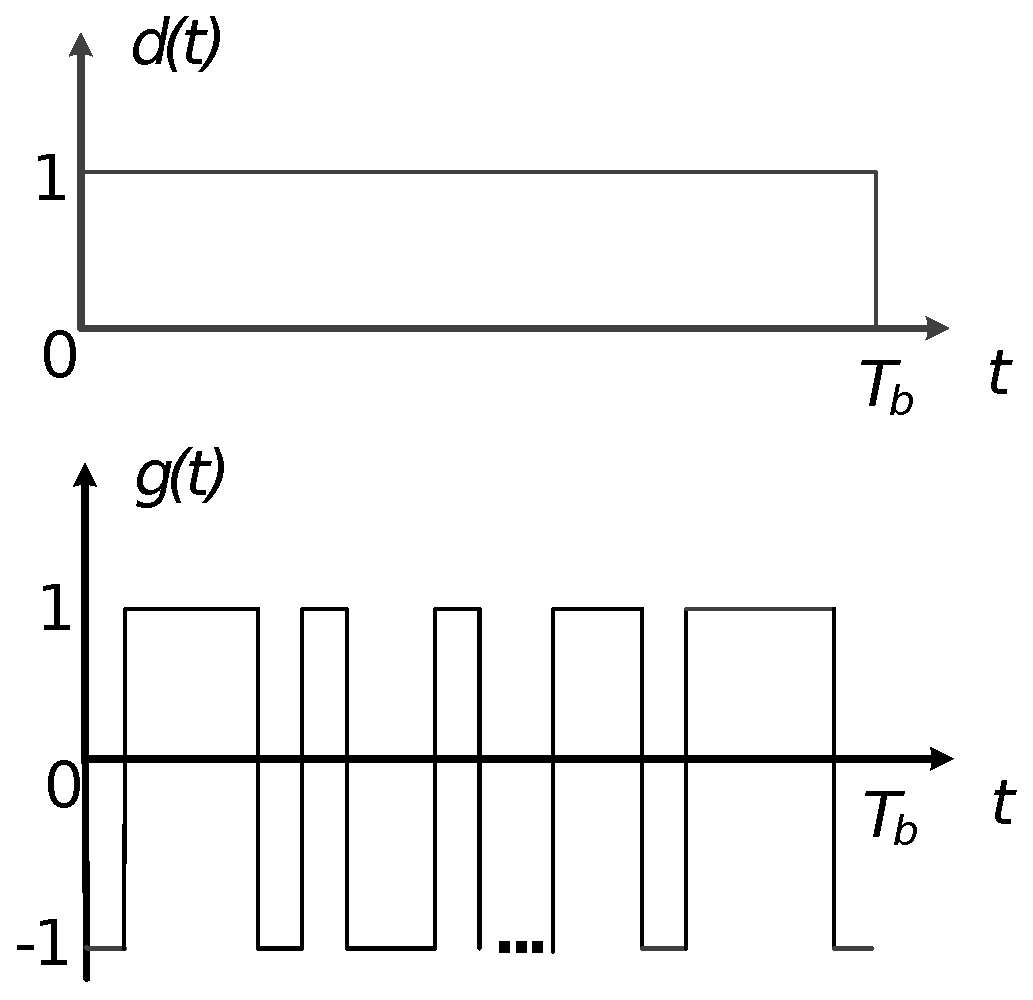
\includegraphics[width=1\linewidth]{bit_and_code.eps}}
	\caption{\\Информационный бит ${d(t)}$ и модулирующая последовательность ${g(t)}$} 
	\label{pic:bit_and_code}
\end{figure}

Таким образом, сигнал на выходе модулятора может быть представлен \cite{shahtarin_sync}:
\begin{equation}
	\label{eq:cdma_eq}
	s(t)=Ad(t)g(t)\cos{(\omega_{0}t)},
\end{equation}
где ${A}$ - амплитуда, ${d(t)}$- информационный бит, а ${g(t)}$ - ПСП.

Как уже было отмечено, при данном методе
расширение спектра достигается за счет модуляции несущей частоты, чаще всего двоичной ПСП, или за счет псевдослучайной перестройки рабочей частоты \cite{borisovBook}.
Рассматриваемое в работе семейство ПСП Голда относится к ПСП, модулирующей сигнал при помощи псевдослучайной перестройки фазы - фазо-манипупулированный широкополосный сигнал
(ФМШПС). Так как в данной работе не рассматриваются другие виды ПСП, будем заменять термин ФМШПС термином ШПС, принимая во внимание только случай ФМШПС.

Таким образом (\ref{eq:cdma_eq}) может быть также записано как:
\begin{equation}
	\label{eq:cdma_eq_phi}
	s(t)=Ad(t)\cos{(\omega_{0}t + \theta_k)},
\end{equation}
где ${(\theta_k=\alpha_k \pi, \alpha_k \in \{0, 1\})}$.

Амплитуда ${A}$ сигнала зависит от многих факторов и должна рассматриваться как случайная величина \cite{pestryakov-book}. Случайность
амплитуды может иметь разный характер. Обычно амплитуда сигнала неизвестна и может изменяться в широких пределах,
но очень медленно, в зависимости от условий функционирования системы. Большой интерес представляет определение пороговых
значений мощности (амплитуды) или энергии сигнала при заданном уровне помех, обеспечивающих при оптимальном
обнаружении требующуюся достоверность обнаружения или передачи сообщения. В этих условиях амплитуду сигнала или его энергию
полезно рассматривать как переменную величину и исследовать ее влияние на результат работы системы.

Информационный бит ${d(t)}$ остается постоянным в течении промежутка ${T_b}$:
\begin{equation}
	\label{eq:cdma_eq_data}
	 d(t) = \begin{cases}
		1, 0 \le t \le T_b; \\
		0, t \not\in [0, T_b].
		\end{cases}
\end{equation}

В случае прямоугольной формы символов информационной последовательности двоичной ШПС на длительности одного бита данных, сигнал можно представить как:
\begin{equation}
	\label{eq:cdma_eq_phi}
	s(t)=Ad(t)g(t)\cos{(\omega_{0}t + \theta_0)}, 0 \le t \le T_b,
\end{equation}
где ${\theta_0}$ - начальная фаза сигнала, ее значение имеет равномерное распределение на интервале ${(\theta_0 \in [0, 2\pi])}$.

Известно, что для случайной последовательности (СП) корреляционная функция (КФ) равна:
\begin{equation}
	\label{eq:cdma_ca_corr_func}
	 R_p(\tau) = \begin{cases}
		1 - \frac{|\tau|}{\tau_c}, |\tau| < \tau_c; \\
		0, |\tau| > \tau_c.
		\end{cases}
\end{equation}

График КФ СП имеет вид Рис. \ref{pic:cf_code}.
\begin{figure}[h]
	\center\scalebox{0.7}{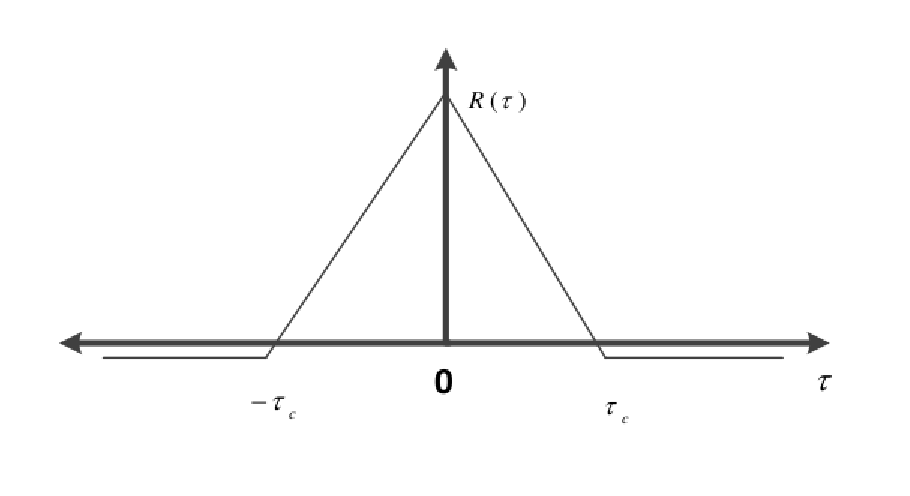
\includegraphics[width=1\linewidth]{cf_code.eps}}
	\caption{График КФ СП} 
	\label{pic:cf_code}
\end{figure}

СПМ ${G_p(f)}$ центрированного СП по теореме Винера-Хинчина является преобразованием Фурье
от КФ \cite{borisovBook}:
\begin{align}
	\label{eq:psd_corr_func}
	G_p(f) & = & \int^{\inf}_{inf} R(\tau)e^{-j2\pi f \tau} d\tau = \int^{\inf}_{inf} \left( 1 - \frac{|\tau|}{\tau_c} \right) e^{-j2\pi f \tau} d\tau = \nonumber \\
		& = & \int^{\tau_c}_{0}\left( 1 - \frac{|\tau|}{\tau_c} \right) \cos{(2\pi f \tau)} d\tau = \tau_c \left( \frac{\sin{(\pi f \tau_c)}}{\pi f \tau_c} \right)^2.
\end{align}

Выражение (\ref{eq:psd_corr_func}) представляет собой СПМ произведения ${p(t)d(t)}$ при использовании случайного сигнала ${p(t)}$.

Из литературы по теории автоматических систем, например \cite{pugachev}, известна классическая постановка
задачи теории оптимальных систем. "На практике часто приходится решать задачу проектирования системы, когда
требуется определить характеристики системы таким образом, чтобы она имела наибольшую точность при данных условиях.
Систему, обеспечивающую наибольшую возможную точность с какой-нибудь определенной точки зрения среди всех систем
заданного класса, обычно называют оптимальной" \cite{pugachev}.

В одной из постановок данной задачи \cite{pugachev}, система считается полностью неизвестной
и требуется определить ее оператор так, чтобы она была оптимальной с точки зрения принятого критерия качества. Эта
задача сводится к определению с наибольшей возможной точностью некоторых параметров, от которых зависит принимаемый
сигнал. Но при этом важно учитывать не только точность, но и другие факторы, так как проектируемая система должна
удовлетворять многим, часто противоречивым требованиям. В виду приведенных факторов, обычно представляет собой
ряд компромиссных решений, удовлетворяющих всем предъявляемым к системе требованиям.

Точность автоматической системы обычно характеризуется математическим ожиданием и дисперсией ее ошибки.
Математическое ожидание представляет собой систематическую ошибку системы в данных условиях, а дисперсия
характеризует уровень случайных ошибок \cite{pugachev}. Так как в различных условиях работы
различных систем, систематическая ошибка тоже является случайной, за критерий качества
системы при ее проектировании обычно принимают второй начальный момент ошибки - математическое ожидание
квадрата ошибки:
\begin{equation}
	\label{eq:stat_err_prob}
	\eta = M[e^2(t)].
\end{equation}

Положительный квадратный корень из этой величины называют средней квадратической ошибкой  (СКО) системы. Таким образом,
оптимальной системой обычно считают такую систему, которая имеет минимальную среднюю квадратичную ошибку.

Критерий минимума СКО является простейшим с математической точки зрения и обычно приводит
к наиболее простым методам определения оптимальных систем. Следует отметить, что далеко не во всех задачах он может служить мерой
качества системы. 

В случаях, когда необходимо проектировать следящую систему, приходится учитывать возможность срыва слежения,
который заключается в том, что система перестает работать, если ее ошибка превосходит по абсолютной величине некоторый
уровень. При проектировании таких систем целесообразно принять за критерий качества вероятность срыва слежения. При
этом оптимальной считается такая система, которая обеспечивает минимум вероятности срыва слежения. Если срыв слежения
происходит в случае, когда абсолютная величина ошибки превосходит уровень $a$, то критерий минимума вероятности ошибки
слежения можно представить \cite{pugachev}:
\begin{equation}
	\label{eq:prob_lost_signal}
	p = P(e(t) > a) = \mbox{min}.
\end{equation}

Оценка параметров сигнала всегда происходит в условиях действия помех и, решая задачу оптимизации приема,
необходимо иметь в виду определенные модели помех. Основной помехой является флуктуационная с нормальным
распределением мгновенных значений и широким равномерным энергетическим спектром. Такие помехи характеризуются
плотностью мощности ${\sigma_n^2}$ на входе схемы обработки \cite{pestryakov-book}.

Вторым видом помех, оказывающих
большое влияние на прием сигналов, являются помехи, связанные с рассеянным или многолучевым распространением
радиосигналов. Многолучевое распространение радиоволн можно рассматривать двояко: или как фактор, обуславливающий
наличие дополнительных помех в виде сигналов, аналогичных тому, который рассматривается как основной, но с другой
задержкой; или как фактор изменяющий статистические характеристики параметров принимаемого сигнала,
обуславливая случайность амплитуды \cite{pestryakov-book}.

Третьим видом помех, характерных для систем связи, использующих ШПС, являются помехи от шумоподобных сигналов,
принадлежащих другим адресам (каналам). Эти помехи определяются тем, что при использовании ШПС для разделения
сигналов по форме (кодовое разделение), сигналы, принадлежащие другим адресам, не являясь идеально ортогональными,
создают помехи. Сумма нескольких шумоподобных сигналов дает результирующий процесс, близкий к нормальному шуму,
поэтому помеху, создаваемую многими ШПС, почти всегда можно рассматривать как нормальный шум с ограниченным
равномерным спектром и ограниченной мощностью \cite{pestryakov-book}.

Мощность АБГШ подвергается значительным изменениям. Это обусловлено
изменением собственных шумов приемника, помехами, создаваемыми атмосферой и космосом, усилением приемного устройства
и т.п. Следовательно, для АБГШ плотность мощности ${N_n}$ является случайной величиной.

В системе Navstar GPS можно выделить 6 источников помех \cite{parkinson_1996}:
\begin{itemize}
	\item {данные эфемерид - ошибки в позициях спутников;}
	\item {часы спутника - ошибки в переданных данных о времени;}
	\item {ионосфера - ошибки в коррекции псевдодальностей, обусловленных ионосферными эффектами;}
	\item {тропосфера - ошибки в коррекции псевдодальностей, обусловленных тропосферными эффектами;}
	\item {многолучевость - эффект отраженных сигналов, принятых антенной;}
	\item {приемник - ошибки в измерениях обусловленные термальным шумом, точностью программного обеспечения (ПО) и т.д.}
\end{itemize}

Так как приведенные выше виды помех влияют только на точность определения координат, мы можем рассматривать упрощенную модель
канала, где данные виды помех не рассматриваются отдельно. В данной работе рассмотрены помехи, обусловленные интерференционной помехой и АБГШ. 
Более углубленные модели канала можно найти в
источниках: упрощенная модель канала с сигналом на промежуточной частоте \cite{lei_dong_phd}, модель многолучевого
распространения \cite{hannah_phd}, а также \cite{burns_model, corbell_model, brown_model}.

\section{Алгоритм оптимальной оценки параметров ШПС}
Алгоритм реализующий метод максимального правдоподобия - последовательный коррелятор. Данный подход реализуется в аппаратных приемниках.
Аппаратный приемник позволяет реализовать параллельно несколько последовательных корреляторов и вести оценку параметров
СПИ с ШПС параллельно.

Данный алгоритм в некоторых источниках также называется согласованным фильтром. В \cite{sklyar} рассмотрены нюансы этих двух понятий.
В данной работе используется понятие последовательный коррелятор. Работа коррелятора описывается математической операцией
корреляции:
\begin{equation}
	\label{eq:serial_corr}
	z(m)=\sum\limits_{n=0}^{N-1}{x(n)h(m+n)},
\end{equation}
где ${x(n)}$ - принятая смесь, а ${h(m)}$ не импульсная характеристика системы, а локальная копия сигнала.

Сигнал коррелируется с локальной копией и на выходе коррелятора получается значение, отражающее
степень совпадения сигналов. Не трудно представить, что сигнал с хорошими корреляционными свойствами должен обладать высоким значением
корреляции, когда сигналы синхронизированы, и минимальным значением в любом другом случае (фаза ПСП не выровнена - отсутствие сигнала).

%%%%%%%%
% DFT

Вычисление циклической свертки через дискретное преобразование Фурье (ДПФ) - достаточно популярный метод
в программных приемниках, так как позволяет существенно уменьшить количество операций при вычислении. Как показано
в \cite{tsui, oppenheim}, можно достаточно просто перейти от свертки к циклической корреляции. Так как этот метод является самым
популярным в программных приемниках стоит его представить.
Свертка может быть представлена как:
\begin{equation}
	\label{eq:fft_conv}
	y(m)=\sum\limits_{n=0}^{N-1}{x(n)h(m-n)}.
\end{equation}

Стоит отметить, что в (\ref{eq:fft_conv}) сдвиг во времени является циклическим, поскольку дискретные операции являются циклическими.
Возьмем ДПФ от (\ref{eq:fft_conv}):
\begin{eqnarray}
	\label{eq:fft_conv_fft}
	Y(k) & = & \sum\limits_{n=0}^{N-1}\sum\limits_{m=0}^{N-1}{x(m)h(n-m)e^{(-j2\pi{kn})/N}}=\nonumber \\
	& = & \sum\limits_{m=0}^{N-1}{x(m)}[\sum\limits_{n=0}^{N-1}h(n-m)e^{(-j2\pi{(n-m)}k)/N}]e^{(-j2\pi{m}k)/N}=\\
	& = & H(k)\sum\limits_{m=0}^{N-1}e^{(-j2\pi{m}k)/N} = X(k)H(k)\nonumber.
\end{eqnarray}

Из уравнения (\ref{eq:fft_conv_fft}) легко видеть, что это нелинейная свертка. В линейной свертке для входного сигнала размером в ${N}$ точек,
результат будет из ${2N-1}$ точек. А в (\ref{eq:fft_conv_fft}), результатом является всего ${N}$ точек.
Это проявление циклической природы ДПФ.

Алгоритм оценки не использует свертку, он использует корреляцию, которая отличается от свертки. Корреляция
между $x(m)$ и $h(m)$ записывается выражением (\ref{eq:serial_corr}).
Единственным отличием между выражениями (\ref{eq:serial_corr}) и (\ref{eq:fft_conv}) является знак перед $n$ в ${h(m+n)}$.
В случае оценки параметра ШПС, $h(m)$ является локальной копией сигнала, а не импульсной характеристикой. Результат ДПФ от (\ref{eq:serial_corr}):
\begin{eqnarray}
	\label{eq:fft_corr_fft}
	Z(k) & = & \sum\limits_{n=0}^{N-1}\sum\limits_{m=0}^{N-1}{x(m)h(n+m)e^{(-j2\pi{kn})/N}}=\nonumber \\
	& = & \sum\limits_{m=0}^{N-1}{x(m)}[\sum\limits_{n=0}^{N-1}h(n+m)e^{(-j2\pi{(n+m)}k)/N}]e^{(j2\pi{m}k)/N}=\\
	& = & H(k)\sum\limits_{m=0}^{N-1}e^{(j2\pi{m}k)/N} = X(k)H^{-1}(k)\nonumber,
\end{eqnarray}
где ${X^{-1}(k)}$ - обратное ДПФ. Выражение (\ref{eq:fft_corr_fft}) можно записать как:

\begin{equation}
	\label{eq:fft_corr_fft_rev}
	Y(k) = \sum\limits_{n=0}^{N-1}\sum\limits_{m=0}^{N-1}{x(n+m)h(m)e^{(-j2\pi{kn})/N}}=X^{-1}(k)H(k).
\end{equation}

Если сигнал $x(n)$ действительный, то $x(n) = x^*(n)$, где ${^*}$ - операция комплексного сопряжения. Используя данное соотношение,
значение $Z(k)$ может быть записано:
\begin{equation}
	\label{eq:fft_magnitude}
	|Z(k)|=|H^*(k)X(k)|=|H(k)X(k)^*|.
\end{equation}
Данное соотношение может быть использовано для нахождения значения циклической корреляции между входным сигналом и 
локальной копией.

\section{Алгоритм оценки информационных параметров ШПС на фоне АБГШ c использованием АР-модели}
%Спектральный анализ - это один из методов обработки сигналов, который позволяет охарактеризовать частотный состав измеряемого сигнала.
%Методы статистики играют важную роль в спектральном анализе, поскольку сигналы, как правило, имеют шумовой или случайный характер. Если бы
%основные статистические характеристики сигнала были известны точно или же их можно было бы без ошибок определить на конечном интервале этого
%сигнала, то спектральный анализ представлял бы собой отрасль точной науки. В действительности по одному-единственному отрезку сигнала можно
%получить только некоторую оценку его спектра. Практика спектрального анализа после 1880-х гг. постепенно стала превращаться в некое ремесло
%достаточно субъективного характера, которое на ряду с использованием научного подхода требовало также определенного уровня эмпирического
%искусства \cite{marpl_book}.
%
%В 1927 г. Дж. Юл предложил существенно новый метод спектрального анализа. Для отыскания одной-двух периодичностей в исследуемых данных Юл
%прибег к моделированию временного ряда, основанному на линейном регрессионном анализе. Юла интересовала главным образом более высокая точность
%определения основной периодичности в ряде чисел солнечных пятен и отыскания в нем дополнительных периодичностей \cite{marpl_book}.
%Используя простое тригонометрическое тождество:
%\begin{equation}
%	\label{eq:yule_trigonometric}
%	\sin(kx)=2\cos(x)\sin([k-1]x)-sin([k-2]x)
%\end{equation}
%Используя подстановки и обобщая формулу (весь ход обобщения описан в \cite{marpl_book}) можно получить:
%\begin{equation}
%	\label{eq:yule_raznost}
%	u(k) = a(1)u(k-1) + a(2)u(k-2) + \epsilon (k)
%\end{equation}
%Здесь ${u(k) = \sin (2\pi fkT)}$ - гармоническая составляющая, ${T}$ - интервал отсчетов, ${f}$ - частота гармоники,
%${\epsilon (k)}$ - некоторое малое импульсное возмущение, а ${a(1)}$ и ${a(2)}$ принимают произвольные значения.
%Как легко увидеть, выражение \ref{eq:yule_raznost} представляет собой АР уравнение. Юл предположил, что
%если процесс имеет только один тон, то он может быть описан как \ref{eq:yule_raznost}.
%решением уравнения \ref{eq:yule_raznost} является затухающая синусоида.

АР-модель предсказания отсчета может быть описана как взвешенная сумма ${P}$ предыдущих отсчетов сигнала \cite{marpl_book}:
\begin{equation}
	\label{eq:lpc_forecast}
	\hat{s}(m) = \sum \limits_{k=1}^P a_k s(m-k),
\end{equation}
где ${\hat{s}(m)}$ - оценка ${s(m)}$ в момент времени ${m}$, а ${a_k}$ - коэффициенты АР-модели, ${P}$ - порядок модели.

АР-модель может быть использована для оценки частоты в ШПС. При этом, если обрабатывается ШПС от нескольких источников,
оценка спектра будет смещенной и требуется ее корректировка. После повторной модуляции
с синхронизированной копией ПСП получается гармоническая компонента на промежуточной частоте и шум. 
В выражении (\ref{eq:cdma_eq_phi}) примем ${A = 1}$, ${D_k(t)=1}$, учитывая, что мы оцениваем параметры сигнала в пределах одной
ПСП:
\begin{equation}
	\label{eq:lpc_signal}
	x(t) = \cos(\omega_{0}t + \theta(t)) + n(t).
\end{equation}

Для выражения (\ref{eq:lpc_signal}), необходимо записать ковариации для трех точек
${r_{xx}(0)}$, ${r_{xx}(1)}$, ${r_{xx}(2)}$:
\begin{equation}
	\label{eq:lpc_cov}
	{r_{xx}(\tau) = \frac{1}{N} \sum \limits_{n=0}^{N-1} x(n) x(n-\tau)}.
\end{equation}

Для применения АР-метода важно знать модель шумовой компоненты ${n(t)}$ из выражения
(\ref{eq:lpc_signal}). Зная АКФ ${n(t)}$, можно получить несмещенную оценку ${\omega_0}$.

Ошибка предсказания ${e(m)}$ может быть представлена как:
\begin{equation}
	\label{eq:lpc_error}
	e(m) = x(m) - \hat{x}(m) = x(m) - \sum \limits_{k=1}^P a_k x(m-k).
\end{equation}

Из уравнения (\ref{eq:lpc_error}) смоделированный сигнал может быть представлен следующим рекурсивным соотношением:
\begin{equation}
	\label{eq:lpc_signal_from_ar}
	x(m) = \sum \limits_{k=1}^P a_k x(m-k) + e(m).
\end{equation}

Выражение (\ref{eq:lpc_error}) представляет собой цифровой фильтр.
После ${z}$ - преобразования выражение (\ref{eq:lpc_error}) может быть записано как \cite{saeed_book}:
\begin{eqnarray}
	\label{eq:lpc_z}
		H(z)	& = & \frac{X(z)}{U(z)} = \frac{G}{1 - \sum \limits_{k=1}^P a_kz^{-k}} =  \nonumber \\
			& = & G\frac{1}{\prod \limits_{k=1}^N (1-r_kz^{-1})} \frac{1}{\prod \limits_{k=1}^M (1-2r_k \cos \phi_k z^{-1} + r_k^2z^{-2})}.
\end{eqnarray}

В выражении (\ref{eq:lpc_z}): ${M}$ - пары комплексных полюсов, ${N}$ - действительные полюсы с ${P=N+2M}$,
${r_k}$ и ${\phi_k}$ - радиус и угол ${k}$ - го полюса соответственно. Частотный отклик такой системы 
может быть представлен \cite{saeed_book}:
\begin{eqnarray}
	\label{eq:lpc_freq_resp}
		H(f)	& = & = \frac{G}{1 - \sum \limits_{k=1}^P a_k e^{-j2 \pi kf}} =  \nonumber \\
			& = & G\frac{1}{\prod \limits_{k=1}^N (1-r_k e^{-j2 \pi f)}} \frac{1}{\prod \limits_{k=1}^M (1-2r_k \cos \phi_k e^{-j2 \pi f} + r_k^2 e^{-j4 \pi f})}.
\end{eqnarray}

Уравнения, соответствующие линейному предсказанию, по своей структуре идентичны уравнениям Юла-Уокера для АР-процесса.
Ввиду этого, существует тесная связь между фильтром линейного предсказания и АР-процессом \cite{marpl_book}.

%На Рис. \ref{pic:lpc_poles} изображено отношение между полюсами и АЧХ рекурсивного фильтра. На частотах, соответствующих полюсам,
%на графике АЧХ присутствуют частотные пики.
Пары комплексных корней могут быть представлены через радиус ${r_k}$ и угол ${\phi_k}$ полюса:
\begin{equation}
	\label{eq:lpc_poles}
	z_k = r_k e^{\pm j \phi_k}.
\end{equation}

Для определения резонансной частоты ${H(z)}$ можно воспользоваться формулой:
\begin{equation}
	\label{eq:lpc_poles_freq}
	\omega_k = arg(z_k).
\end{equation}

%\begin{figure}[h]
%	\center\scalebox{1}{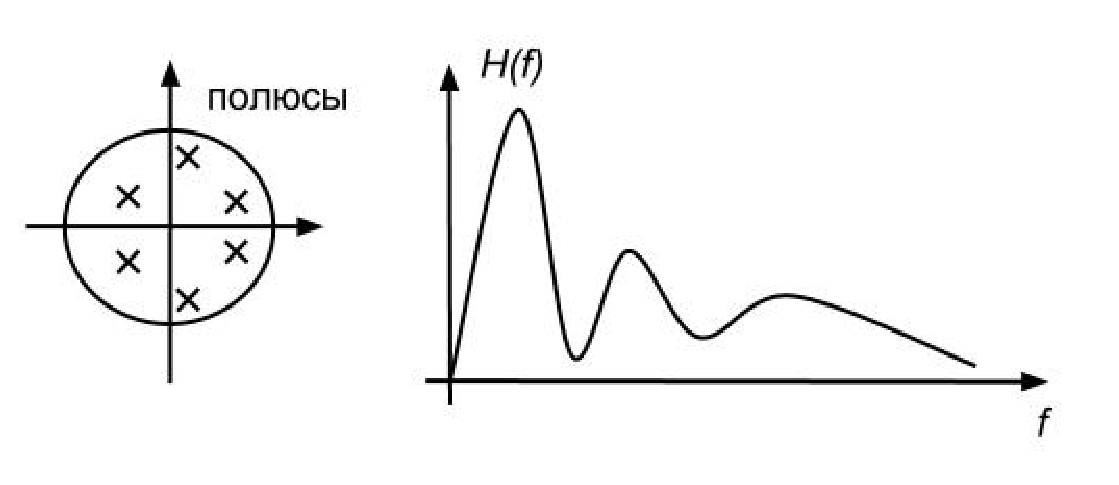
\includegraphics[width=1\linewidth]{lpc_poles.eps}}
%	\caption{Полюса и АЧХ линейного предсказателя}
%	\label{pic:lpc_poles}
%\end{figure}

{\bf{\textit{Вычисление коэффициентов АР-модели}}}

Наилучшие оценки коэффициентов ${a_k}$ могут быть получены минимизацией среднеквадратичной ошибки. Из уравнения (\ref{eq:lpc_error}) \cite{saeed_book}:
\begin{eqnarray}
	\label{eq:lpc_rms}
		E[e^2(m)]	& = & E[(x(m) - \sum \limits_{k=1}^P a_k x(m-k))^2] =\nonumber \\
				& = & E[x^2(m)] - \nonumber \\
				& &  - 2\sum \limits_{k=1}^P a_k E[x(m-k)x(m)] + \nonumber \\
				& &  + \sum \limits_{k=1}^P a_k \sum \limits_{j=1}^P a_j E[x(m-k)x(m-j)] = \nonumber \\
				& = & r_{xx}(0) - 2{\bf r}^T_{xx}{\bf a} + {\bf a}^T {\bf R_{xx}a},
\end{eqnarray}
где ${{\bf R_{xx}} = E[{\bf xx}^T]}$ - автокорреляционная матрица входного \mbox{вектора ${{\bf x}^T=[x(m-1),x(m-2),...,x(m-P)]}$},
${{\bf r}_{xx}=E[x(m){\bf x}]}$ - автокорреляционный вектор, а ${a^T=[a_1,a_2,...,a_P]}$ -  вектор коэффициентов предсказателя.
Процедура минимизации среднеквадратичной ошибки из уравнения (\ref{eq:lpc_rms}) может быть записана как
\begin{equation}
	\label{eq:lpc_rms2}
	{\bf a=R^{-1}_{xx}r_{xx}},
\end{equation}
где матрица ${\bf R_{xx}}$ является теплицевой и эрмитовой, поскольку  ${r_{xx}(-k) = r_{xx}(k)}$.

Данная процедура является реализацией алгоритма Юла-Уокера. В этом алгоритме предполагается, что истинные значения
АКП ${r_{xx}(k)}$ известны. На практике значения АКП не известны и их приходится заменять оценкой ${\hat{r}_{xx}(k)}$, что может
при несмещенных оценках ${\hat{r}_{xx}(k)}$ привести к не положительно определенной матрице ${\bf {R_{xx}}}$, а значит
к неустойчивой \mbox{АР-модели} \cite{bolshakov-book}.

В случае вычисления параметров АР-модели путем решения уравнений \mbox{Юла-Уокера}, нахождение полюсов
внутри единичной окружности не очевидно. В \cite{shahtarin-spectrum-book} показано, что если
автокорреляционная матрица  ${{\bf R_{xx}}}$ является определенной положительно, то и решение
линейных уравнений \mbox{Юла-Уокера} порождает устойчивый только полюсный фильтр.

При больших объемах выборки входных данных, алгоритм Юла-Уокера дает вполне приемлемые результаты, в то время
как при малых выборках оценки параметров дают СПМ с низкой разрешающей способностью \cite{marpl_book, bolshakov-book}.

Можно использовать альтернативную запись.  Для сигнала длинной в ${N}$ отсчетов можно записать ${N}$ - уравнений:
\begin{equation}
	\label{eq:lpc_rms3}
	{\bf e=x-Xa}.
\end{equation}

Выражение (\ref{eq:lpc_rms3}) можно переписать в виде:
\begin{equation}
	\label{eq:lpc_rms4}
	{\bf e^T e = xx^T - 2x^T Xa + a^T X^T Xa}.
\end{equation}

Взяв производную по вектору ${{\bf a}}$, можно получить параметры предсказателя:
\begin{equation}
	\label{eq:lpc_rms5}
	\frac{\partial {\bf e^T e}}{\partial {\bf a}} = {\bf - 2x^T X + a^T X^T X} = 0.
\end{equation}

Из (\ref{eq:lpc_rms5}), коэффициенты для минимальной среднеквадратичной ошибки равны:
\begin{equation}
	\label{eq:lpc_rms6}
	{\bf a= (X^T X)^{-1} (X^T x)}.
\end{equation}

Сравнивая уравнение (\ref{eq:lpc_rms2}) и уравнение (\ref{eq:lpc_rms6}), видно, что в (\ref{eq:lpc_rms2})
автокорреляционная матрица и вектор заменены оценками:
\begin{equation}
	\label{eq:lpc_rxx_estimation}
	\hat{r}_{xx}(m) = \frac{1}{N} \sum \limits_{k=0}^{N-1} x(k)x(k-m).
\end{equation}

Для решения уравнения Юла-Уокера можно применить метод Гаусса, а также его модификации: LU-разложение,
разложение Холецкого, UD-разложение. Данные методы требуют выполнения вычислительных операций, пропорционально ${P^3}$.
Но, так как ${\bf{R^{-1}_{xx}}}$ в (\ref{eq:lpc_rms2}) является теплицевой и эрмитовой, можно использовать эффективные методы работы
с теплицевыми матрицами, которые значительно лучше упомянутых выше. 
Например, можно воспользоваться, быстрым алгоритмом Левинсона-Дарби.
Быстрым алгоритмам над теплицевыми матрицами посвящена книга \cite{bleyhut_book}.

АР-метод оценки СПМ часто используется для того, чтобы выявить в данных наличие синусоидальных
компонент. Мощность, соответствующую  таким компонентам в АР оценке СПМ, можно вычислить, интегрируя
площадь под кривой этой оценки. Однако это связано с большими вычислительными затратами, поэтому
гораздо более эффективным является использования в качестве показателя мощности синусоидальных
компонент высоты соответствующих им спектральных пиков \cite{marpl_book}.  

%%%%%%%%%%%%%%%%%%%%%%%%%%%%%%%%%%%%%%%%%%%%%%%%%%%%%%%%%%%%%%
{\bf{\textit{АР-модель второго порядка. Оценка частоты основного тона на основе АР-модели.}}}

АР-модель второго порядка применяется для определения частоты основного тона. Для поиска единственного
тона необходимо найти два полюса. Тогда выражение (\ref{eq:lpc_rms2}) может быть записано как:
\begin{equation}
	\label{eq:lpc_a_estimation}
	\left[ \begin{array}{c}
		\hat{a}_1 \\
		\hat{a}_2
	\end{array} \right]
	=
		\left[ \begin{array}{cc}
			r_{xx}(0)  + \sigma_n^2 & r_{xx}(1)\\
			r_{xx}^*(1) & r_{xx}(0) + \sigma_n^2 
		\end{array} \right]^{-1}
		\left[ \begin{array}{c}
			r_{xx}(1) \\
			r_{xx}(2)
		\end{array} \right]
	= \bf{R_{xx}^{-1}r_{xx}},
\end{equation}
где ${\hat{a}_1, \hat{a}_2}$, - МНК оценки коэффициентов АР-модели, ${r_{xx}(m)}$ - АКФ принимаемого сигнала.
Для оценки АКФ  можно использовать выражение (\ref{eq:lpc_rxx_estimation}).

Передаточная функция АР-модели второго порядка ${H(z)}$:
\begin{equation}
	\label{eq:lpc_spectral_func}
	H(z) = \frac{1}{1 - a_1 z^{-1} - a_2 z^{-2}}.
\end{equation}

Характеристическое уравнение
\begin{equation}
	\label{eq:lpc_characteristic}
	z^2 - a_1 z - a_2 = 0
\end{equation}
имеет полюсы
\begin{equation}
	\label{eq:lpc_poles_2}
	z_{1,2} =\frac{a_1 \pm \sqrt{a_1^2 + 4 a_2}}{2}.
\end{equation}

Для определения резонансной частоты ${H(z)}$ можно воспользоваться формулой (\ref{eq:lpc_poles_freq}).
Для принятия решения о наличии гармонического сигнала анализируют значение квадрата модуля частотной
характеристики АР-модели в точке резонанса:
\begin{equation}
	\label{eq:lpc_power_cos}
	\left| H(z) \right|^2 = \frac{1}{\left| 1 - a_1 e^{-j \omega_0} - a_2 e^{-2 \omega_0} \right|^2}.
\end{equation}

Если это значение превышает некоторый заранее выбранный порог, то принимается решение о наличии гармонического
сигнала с частотой ${\omega_0}$. 

%%%%%%%%%%%%%%%%%%%%%%%%%%%%%%%%%%%%%%%%%%%%%%%%%%%%%%%%%%%%%%
\section{Использование АР-модели для оценки параметров ШПС}

При работе с ПСП следует учитывать, что после демодуляции входного сигнала выровненной ПСП в сигнале восстанавливается одна гармоническая
компонента на промежуточной частоте, что дает возможность использовать АР-модель второго порядка.
Повторная модуляция сигнала с ПСП по любой фазе, отличной от искомой, не будет восстанавливать гармонический сигнал.
Спектр смеси гармонического сигнала, повторно модулированного ПСП с невыровненной фазой, будет похож на спектр исходной смеси – отображен
на Рис. \ref{pic:lpc_psd_1} штриховой пунктирной линией. И только повторная модуляция с выровненной фазой ПСП даст спектр
изображенный светлой сплошной линией на Рис. \ref{pic:lpc_psd_1}.
\begin{figure}[h]
	\center\scalebox{1}{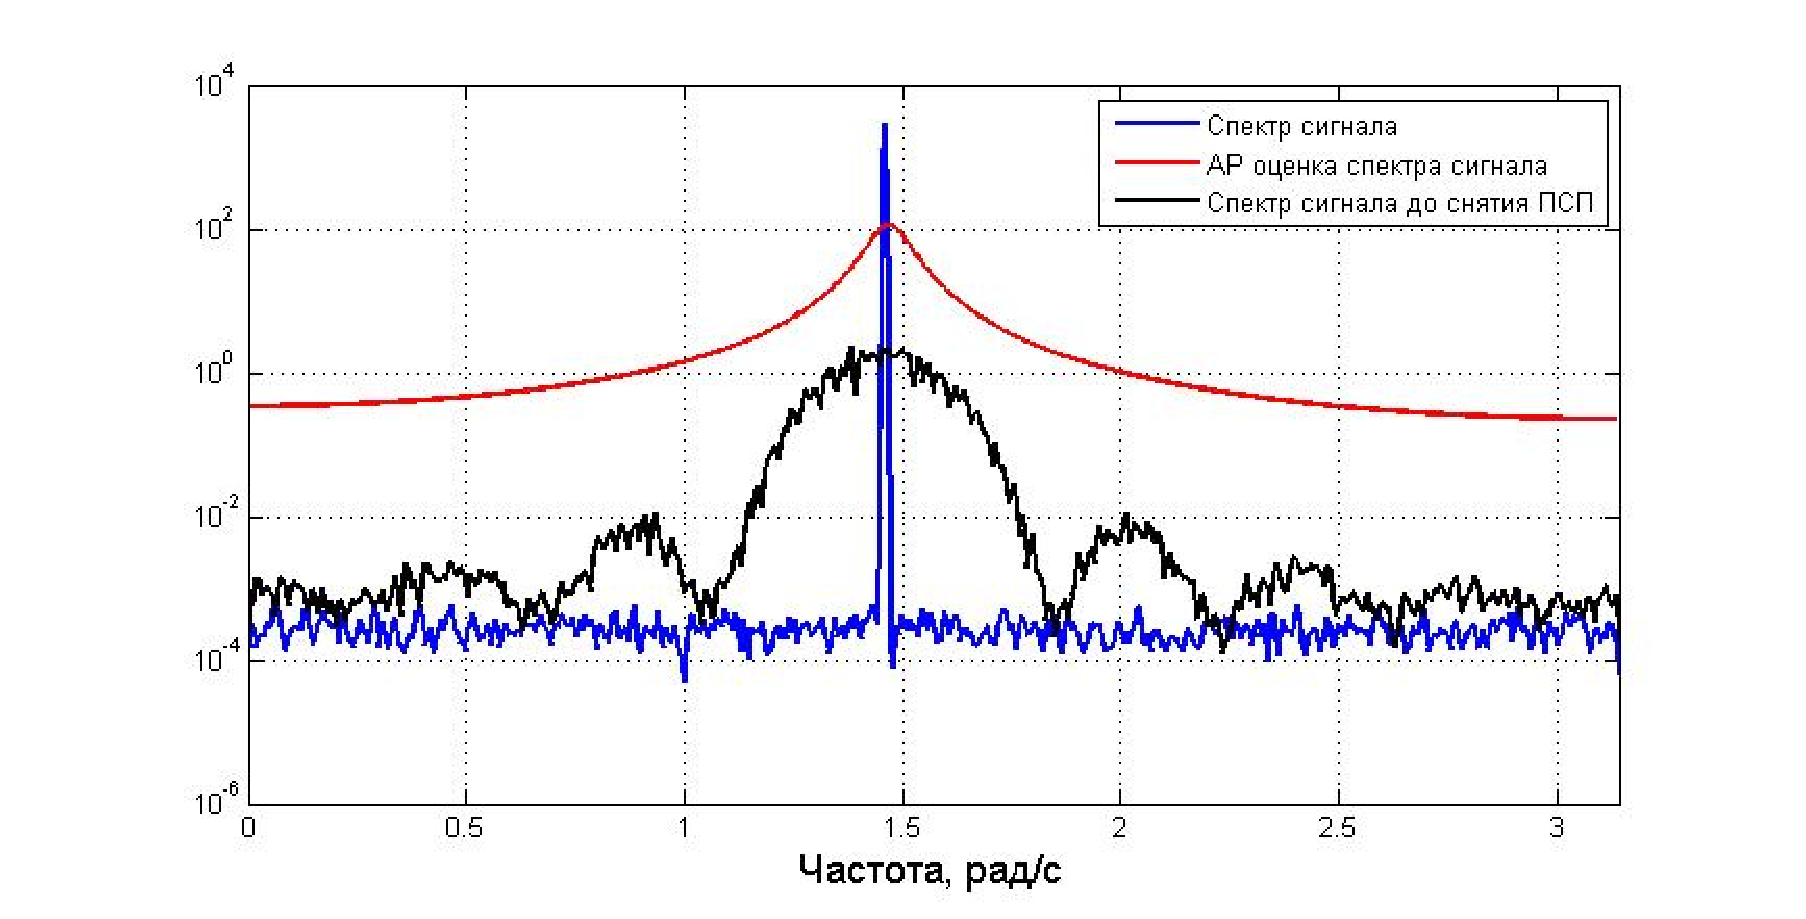
\includegraphics[width=1\linewidth]{lpc_1sat.eps}}
	\caption{Оценка СПМ сигнала, модулированного ПСП}
	\label{pic:lpc_psd_1}
\end{figure}

На \ref{pic:lpc_basic1} входная смесь повторно модулируется ПСП с известной фазой.
\begin{figure}[h]
	\center\scalebox{0.8}{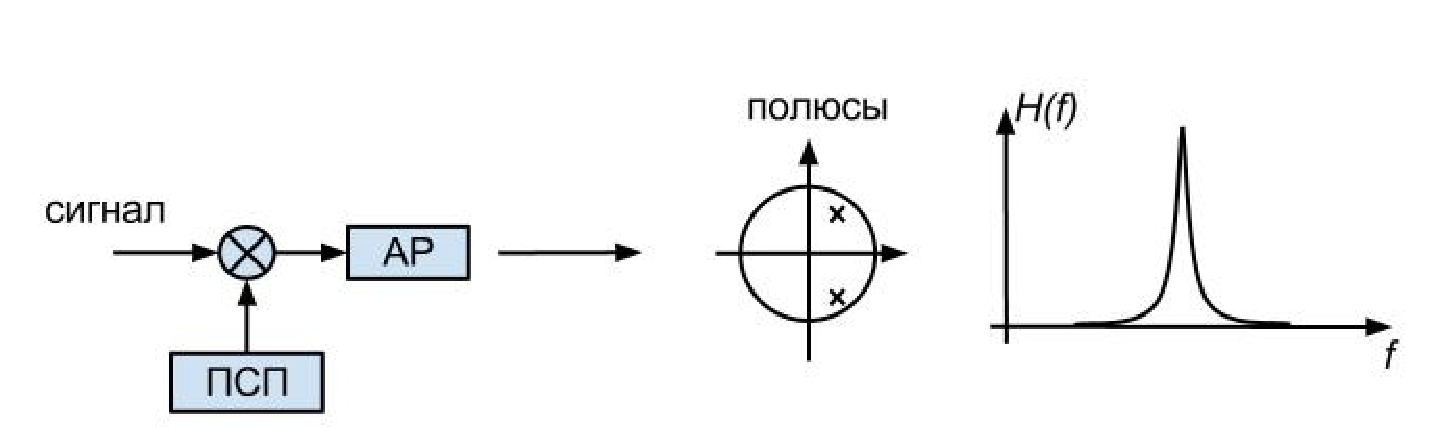
\includegraphics[width=1\linewidth]{lpc_basic.eps}}
	\caption{Общая схема применения АР-модели для детектирования ШПС сигнала}
	\label{pic:lpc_basic1}
\end{figure}

На выходе алгоритма будет СПМ, а пик будет соответствовать энергии на определенной частоте.

%На Рис.  \ref{pic:lpc_poles_gps} красным изображена энергия гармонического колебания с большой мощностью, а зеленым изображен цветной шум.
%\begin{figure}[h]
%	\center\scalebox{1}{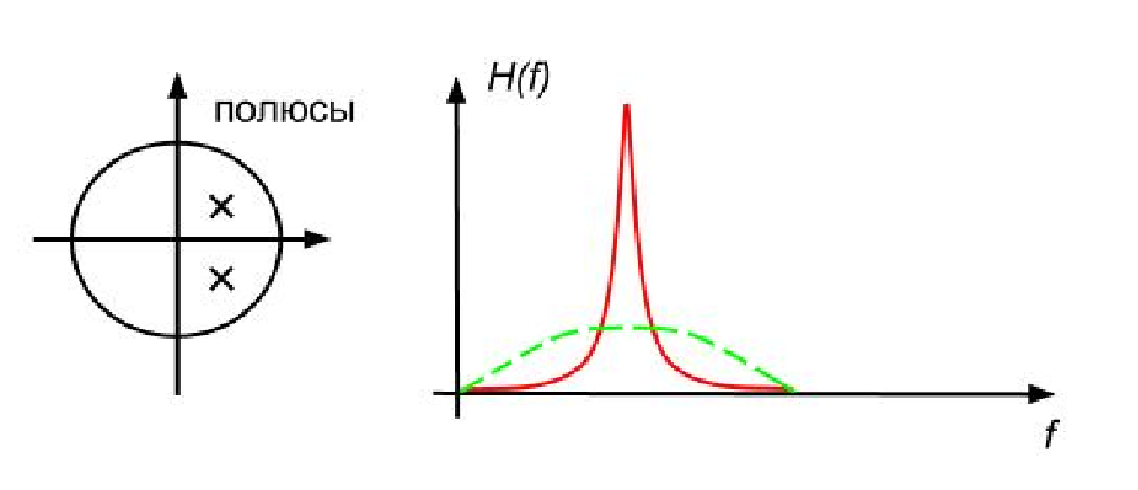
\includegraphics[width=1\linewidth]{lpc_poles_gps.eps}}
%	\caption{Полюс и АЧХ линейного предсказателя}
%	\label{pic:lpc_poles_gps}
%\end{figure}

Так же необходимо отметить, что фаза ПСП в момент начала приема сигнала не известна.
Для оценки частоты сигнала необходимо для каждой фазы ПСП вычислить квадрат частотного
отклика.

Описанный алгоритм состоит из следующих шагов (${\tau \in [0, \tau_{max}]}$):
\begin{itemize}[align=left,style=nextline,leftmargin=*,labelsep=\parindent,font=\normalfont]
\item[Шаг 1.] Вычисляются оценки АКФ в трех точках (для аргументов АКФ=0,1,2)
	для фазы ПСП ${\tau}$, по формуле (\ref{eq:lpc_rxx_estimation}). 
\item[Шаг 2.] Определяются коэффициенты АР-модели ${\hat{a_1}, \hat{a_2}}$, 
	по формуле (\ref{eq:lpc_a_estimation}). 
	Вычисляется резонансная частота ${\omega_0}$ по формуле (\ref{eq:lpc_poles_freq})
	и определяется квадрат модуля частотного отклика АР-модели для этой частоты по выражению (\ref{eq:lpc_power_cos}). 
\item[Шаг 3.] Полученное значение квадрата частотного отклика сравнивается с заранее выбранным порогом детектора. 
	\subitem{\bf{Если}}  значение оказалось больше порогового, {\bf{то}} 
		принимается решение о наличии сигнала, а в качестве оценки
		частоты принимается значение ${\omega_0}$ соответствующее смещению ПСП равному ${\tau}$. 
	\subitem{\bf{Иначе если}} ${\tau}$ меньше длины ПСП ${\tau = \tau + 1}$, переход к шагу 1.
	\subitem{\bf{Иначе}} 
		Принимается решение об отсутствии гармонического сигнала.
\end{itemize}

Квадраты модулей частотного отклика для всех возможных значений фазы в пределах одной ПСП представлены на Рис. \ref{pic:lpc_1sat_energy}.
\begin{figure}[h]
	\center\scalebox{1}{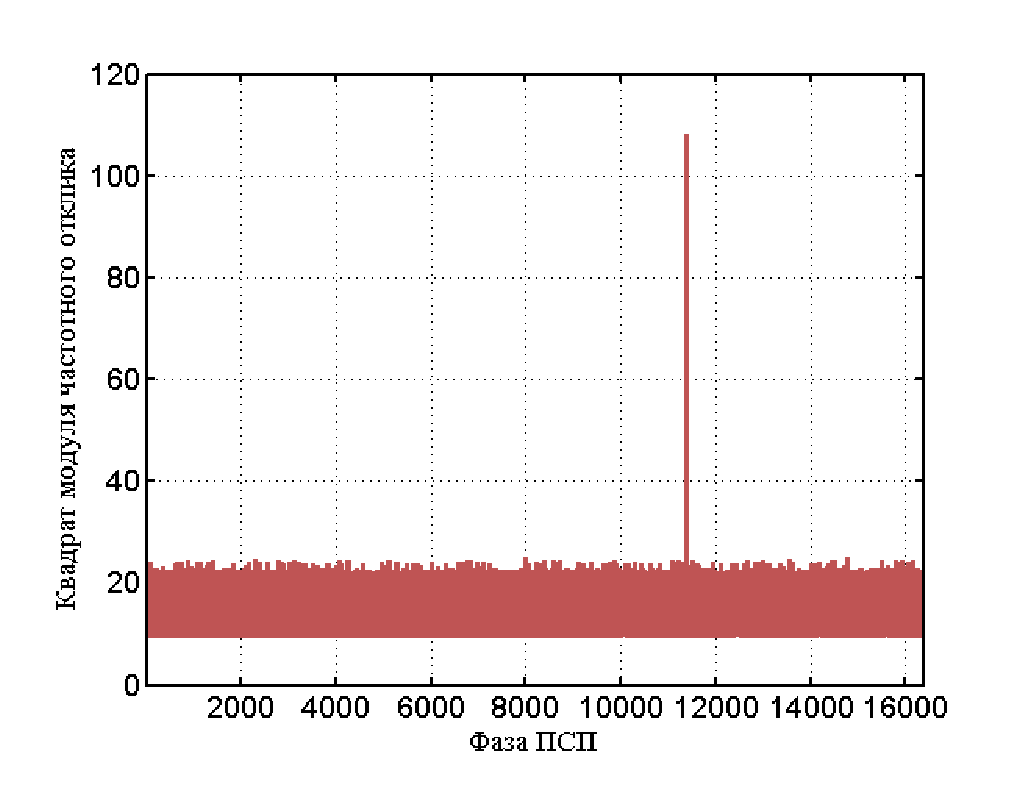
\includegraphics[width=1\linewidth]{lpc_1sat_energy.eps}}
	\caption{Квадраты частотного отклика для всех возможных фаз ПСП}
	\label{pic:lpc_1sat_energy}
\end{figure}

%%%%%%%%%%%%
% My algo

Алгоритм оценки параметров на основе АР-модели требует значительных вычислительных затрат, так как требуется проводить
повторную модуляцию и оценку параметров \mbox{АР-модели} по каждому смещению ПСП.

Для перебора фаз ПСП воспользуемся БПФ, в результате получим значения оценки АКФ для каждой фазы ПСП \cite{my_lpc_for_1, my_lpc_for_1_controllers}.
Схема алгоритма представлена на Рис. \ref{pic:lpc_basic2}. 

\begin{figure}[h]
	\center\scalebox{0.9}{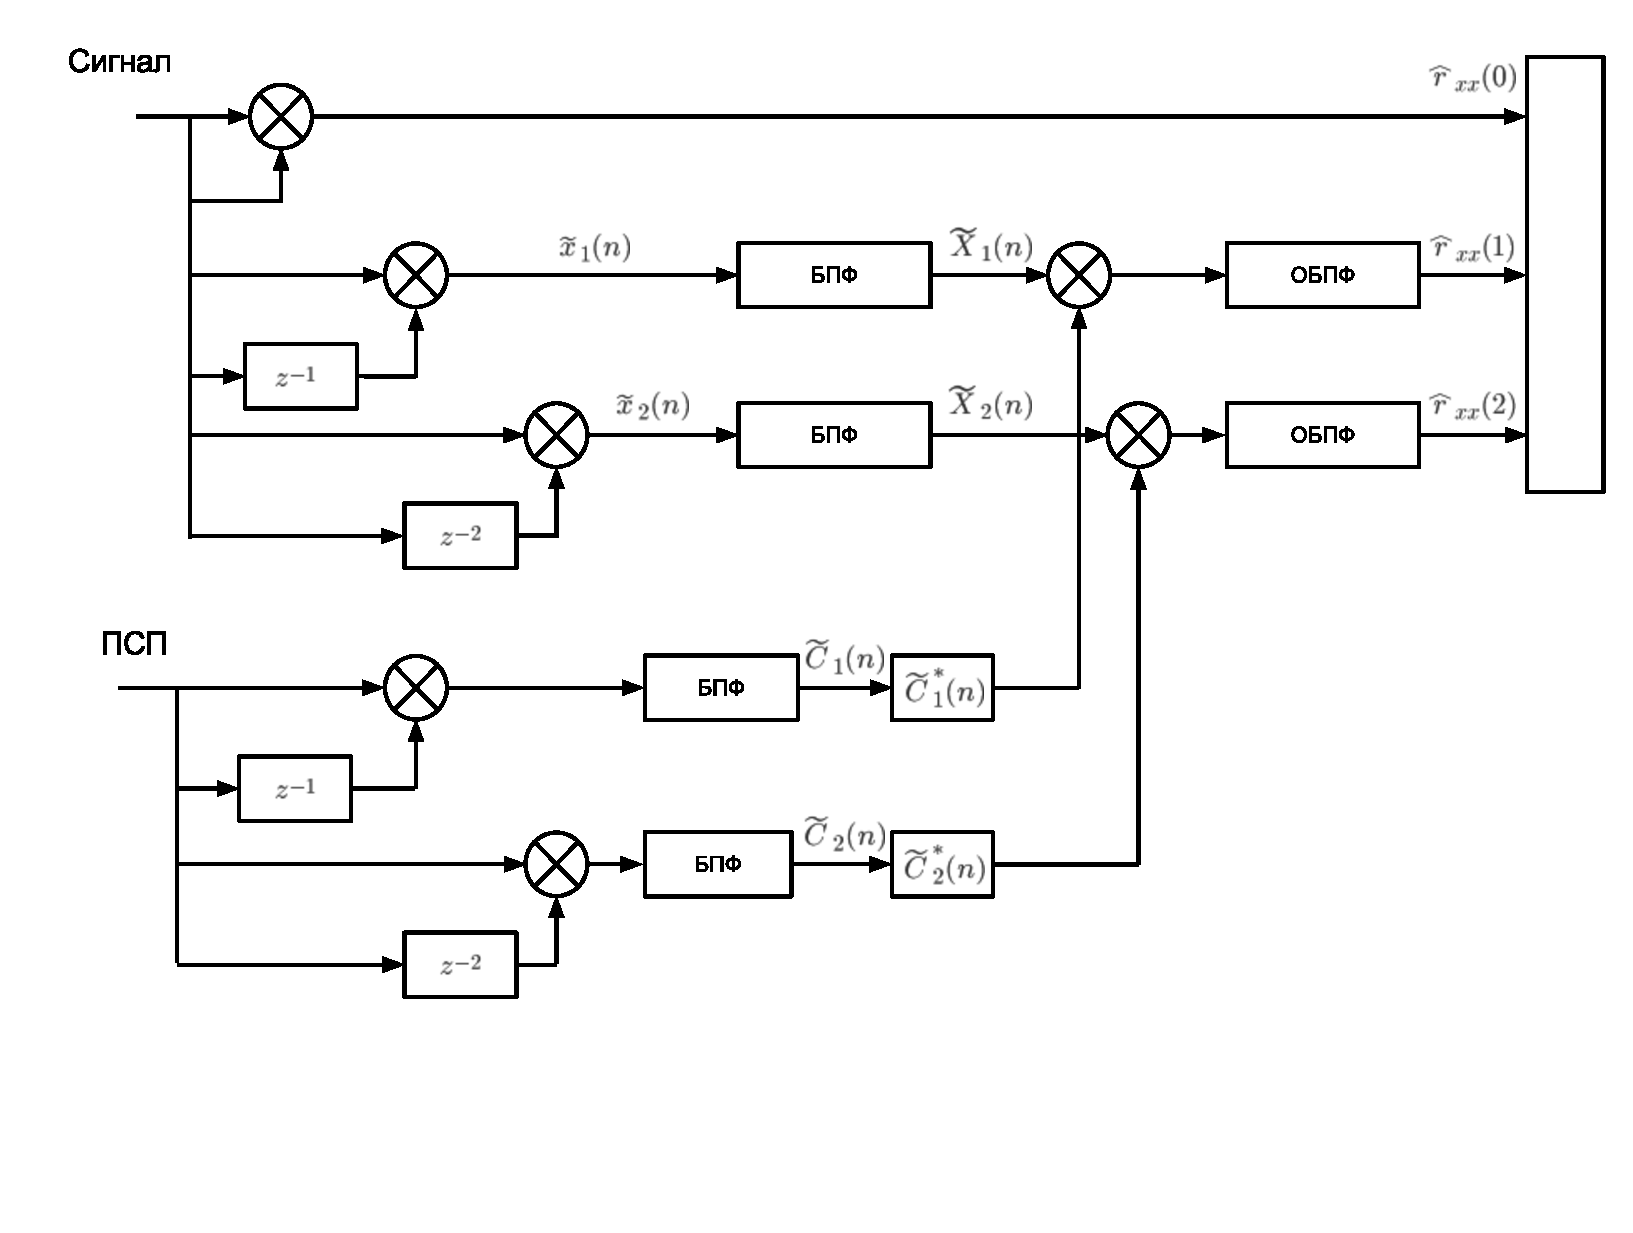
\includegraphics[width=1\linewidth]{lpc_fft.eps}}
	\caption{Схема применения АР-модели для детектирования ШПС сигнала с оптимизацией}
	\label{pic:lpc_basic2}
\end{figure}

Оценка АКФ ${\hat{r}_{xx}(0)}$ не зависит от выбранной фазы ПСП, поэтому она вычисляется один
раз для всех фаз ПСП. Далее формируется массив произведений входной смеси на
свою задержанную копию ${\tilde{x}_1(m)=x(m)x(m-1)}$. Полученная последовательность  
${\tilde{x}_1(m)}$ поступает на вход алгоритма БПФ, в результате получаем массив ${\tilde{X}_1(n)}$.
Аналогично формируется массив  ${\tilde{X}_2(m)}$ для
задержки входной смеси равной двум. Таким же способом обрабатываются локально
сгенерированные ПСП и формируются два массива ${\tilde{G}_1(m)}$ и ${\tilde{G}_2(m)}$.
Далее массивы ${\tilde{X}_1(m)}$ и ${\tilde{X}_1(m)}$ поэлементно перемножаются
на массивы ${\tilde{G}_1^*(n)}$ и ${\tilde{G}_2^*(m)}$, комплексно сопряженные к массивам ${\tilde{G}_1(m)}$ и ${\tilde{G}_2(m)}$.
Результаты этих перемножений поступают на вход алгоритма обратного
БПФ (ОБПФ). Полученные после ОБПФ два массива содержат оценки автокорреляционной функции для ${N}$ 
фаз, где  ${N}$ - размер данных на входе алгоритма БПФ.

Таким образом, предлагаемый алгоритм состоит из следующих шагов:

\begin{itemize}[align=left,style=nextline,leftmargin=*,labelsep=\parindent,font=\normalfont]
\item[Шаг 1.] Вычисляются оценки  АКФ в трех первых точках (для аргументов АКФ=0,1,2)
	с использованием алгоритма БПФ для всех возможных смещений ПСП. 
\item[Шаг 2.] Для каждого смещения ПСП: 
	Определяются коэффициенты АР-модели ${\hat{a_1}, \hat{a_2}}$, 
	по формуле (\ref{eq:lpc_a_estimation}). 
	Вычисляется резонансная частота ${\omega_0}$
	и определяется квадрат модуля частотного отклика АР-модели для этой частоты. 
\item[Шаг 3.] Выбирается смещение ПСП для которого значение квадрата модуля частотного отклика было максимальным. Полученное значение сравнивается с заранее выбранным порогом детектора. 
	\subitem{\bf{Если}}  значение оказалось больше порогового, {\bf{то}} 
		принимается решение о наличии сигнала, а в качестве оценки
		частоты принимается значение ${\omega_0}$ соответствующее выбранному смещению ПСП. 
	\subitem{\bf{Иначе}} 
		Принимается решение об отсутствии гармонического сигнала.
\end{itemize}

Количество операций для оценки параметров от одного источника на фоне АБГШ:
\begin{equation}
	%\label{}
	OP_{AR\_FOR\_1} = 24NlogN + 63N,
\end{equation}
где ${N}$ - длинна входной последовательности.

Вычислительная сложность при использовании типового приемника составляет ${OP_{FFT\_FINE} = 48NlogN + 65N}$
(вывод приводится в Главе 3). Предлагаемый подход позволяет снизить вычислительные затраты в 2 раза в сравнении с типовым подходом.

%%%%%%%%%%%%%%%%%%%%%%%%%%%%%%%%%%%%%%%%%%%%%%%%%%%%%%%%%%%%%%
{\bf{\textit{Влияние теплового шума на точность оценки частоты с помощью АР-модели.}}}

Серьезным фактором, ограничивающим применение АР-модели при оценке параметров гармонического сигнала, является
его чувствительность к шуму. В особенности к окрашенному шуму.

На Рис. \ref{pic:lpc_psd_2} представлена оценка СПМ для ШПС при наличии интерференции.
\begin{figure}[h]
	\center\scalebox{1}{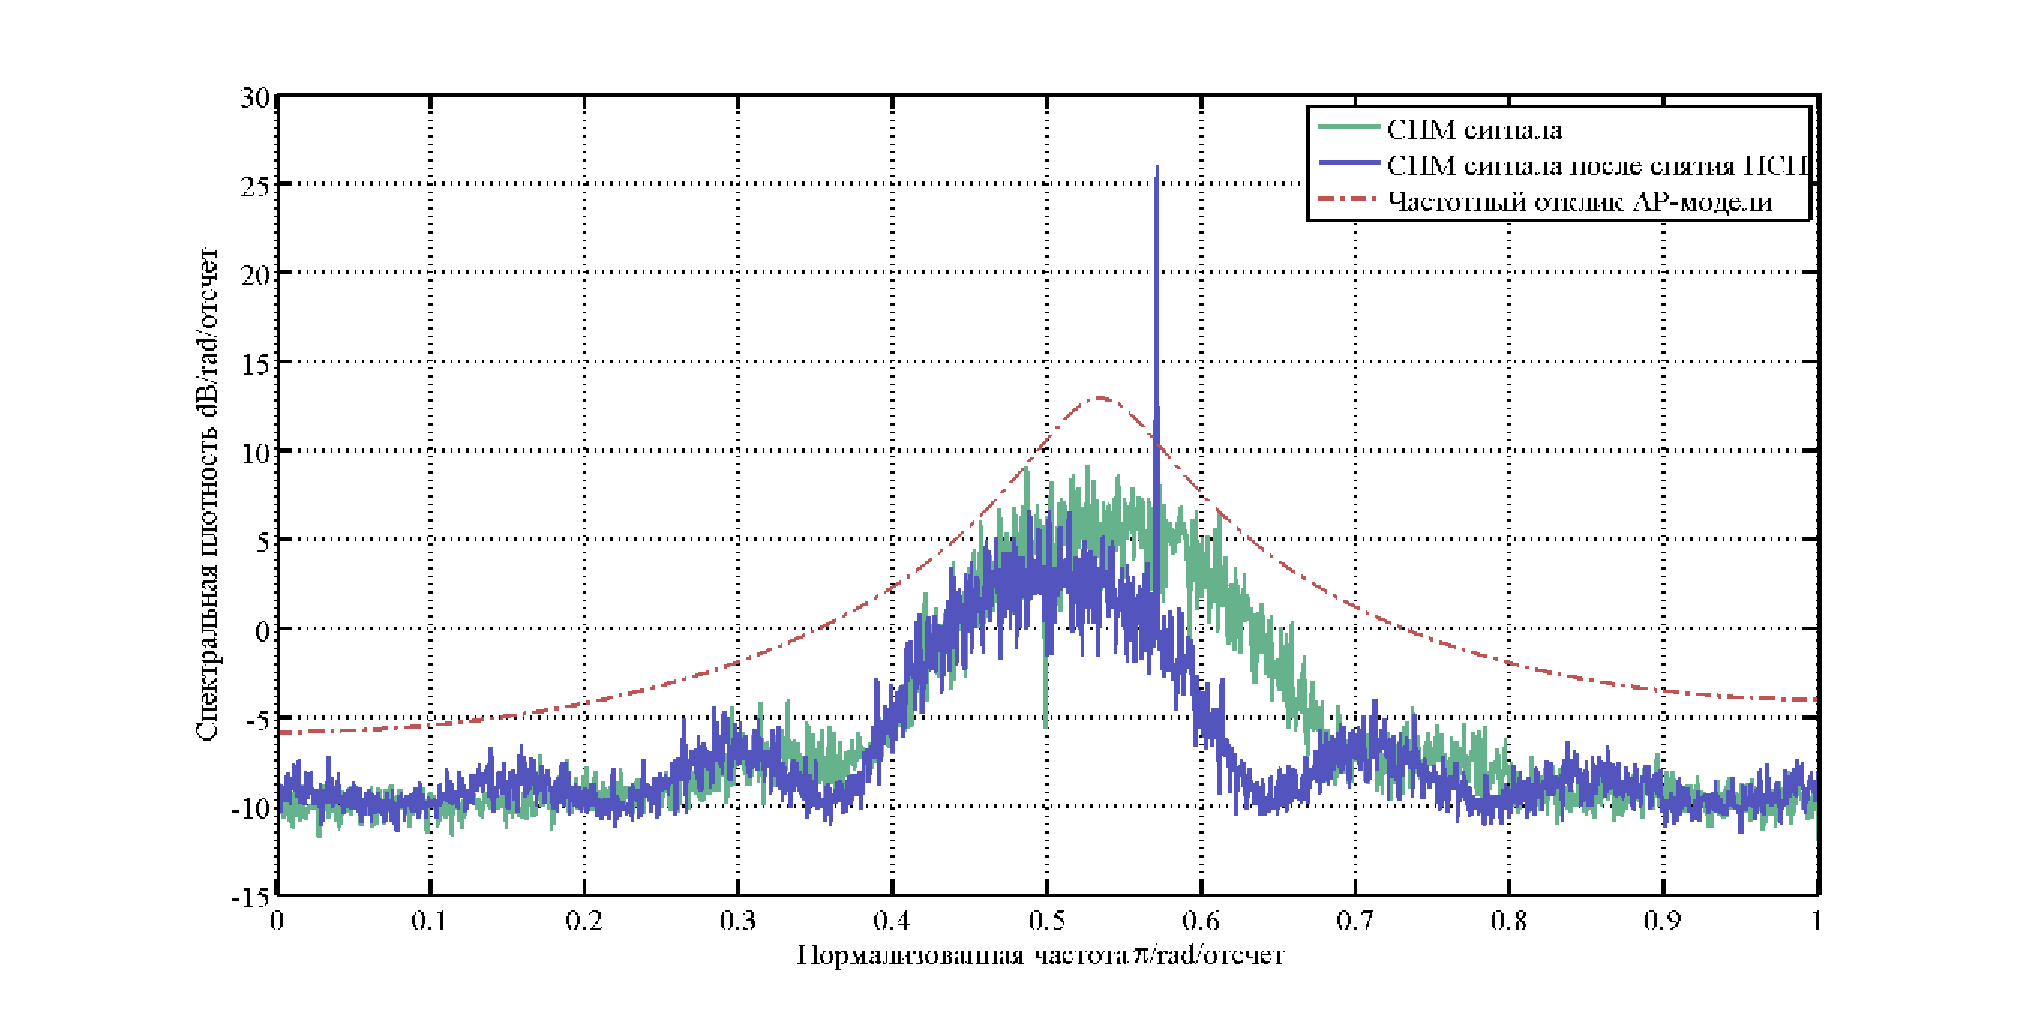
\includegraphics[width=1\linewidth]{lpc_2sat_psd.eps}}
	\caption{\\Оценка СПМ сигнала, модулированного ПСП при наличии интерференционной помехи}
	\label{pic:lpc_psd_2}
\end{figure}

Наличие в данных интерференционной составляющей сильно смещает оценку. Ввиду данного факта, предлагаемый алгоритм в исходном виде
не может быть применен в реальных системах, так как реальные системы обладают множеством каналов, разделенных кодом ПСП. Поэтому предложенный алгоритм,
основанный на \mbox{АР-методе}, нуждается в ряде усовершенствований чтобы удовлетворять критериям реальных систем.

%%%%%%%%%%%%%%%%%%%%%%%%%%%%%%%%%%%%%%%%%%%%%%%%%%%%%%%%%%%%%%
\section{Сравнение точности оценки с границей Крамера-Рао}
График вероятности оценки частоты в допустимом диапазоне входной расстройки модуля фазовой автоподстройки частоты (ФАПЧ) представлен на Рис.
\ref{pic:lpc_for_1_probability}. Моделирование проводилось с аддитивным шумом, заданным в полосе от 0 Гц до
половины частоты дискретизации для одного источника. В данном случае значение частоты дискретизации равно 16.368 МГц.
\begin{figure}[H]
\center\scalebox{1}{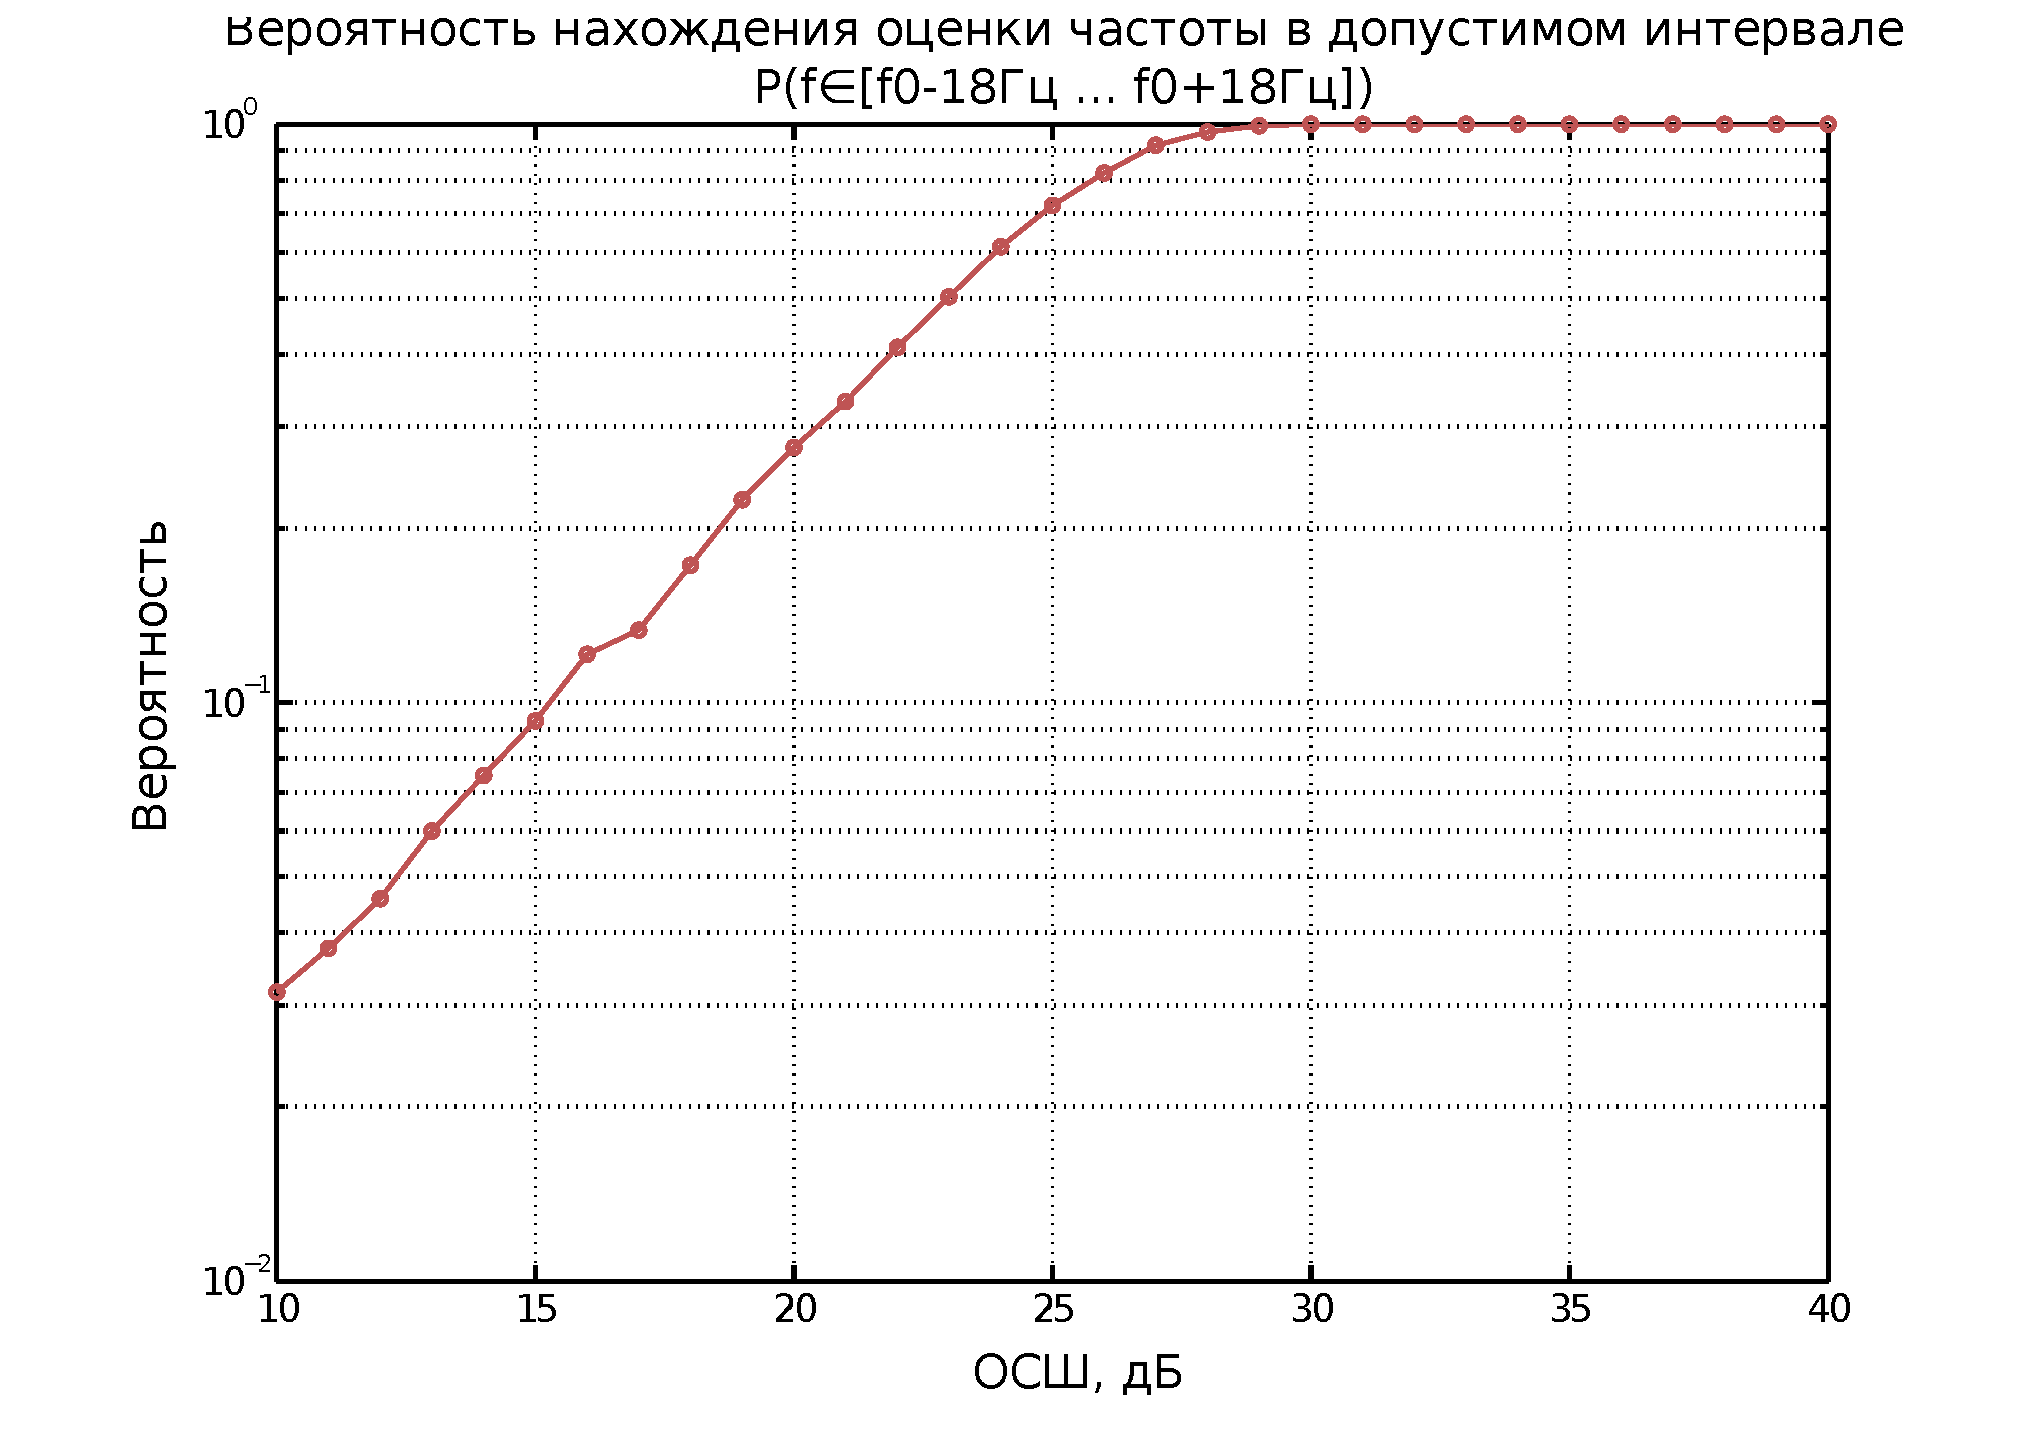
\includegraphics[width=1\linewidth]{lpc_for_1_probability.eps}}
	\caption{\\Вероятность нахождения оценки частоты в интервале, удовлетворяющем допустимой входной расстройке ФАПЧ}
	\label{pic:lpc_for_1_probability}
\end{figure}

Математическое моделирование показало, что удовлетворительное значение вероятности нахождения частоты в полосе, удовлетворяющей допустимой
входной расстройке ФАПЧ \mbox{(Рис. \ref{pic:lpc_for_1_probability})}, достигается при уровне \mbox{25 дБ}.

Для оценки точности можно сравнить предлагаемый алгоритм с границей Крамера-Рао (КР). Неравенство Крамера-Рао дает базу оценки, так
как представляет минимальную дисперсию оцениваемой величины среди всех классов оценщиков.
\begin{figure}[H]
\center\scalebox{1}{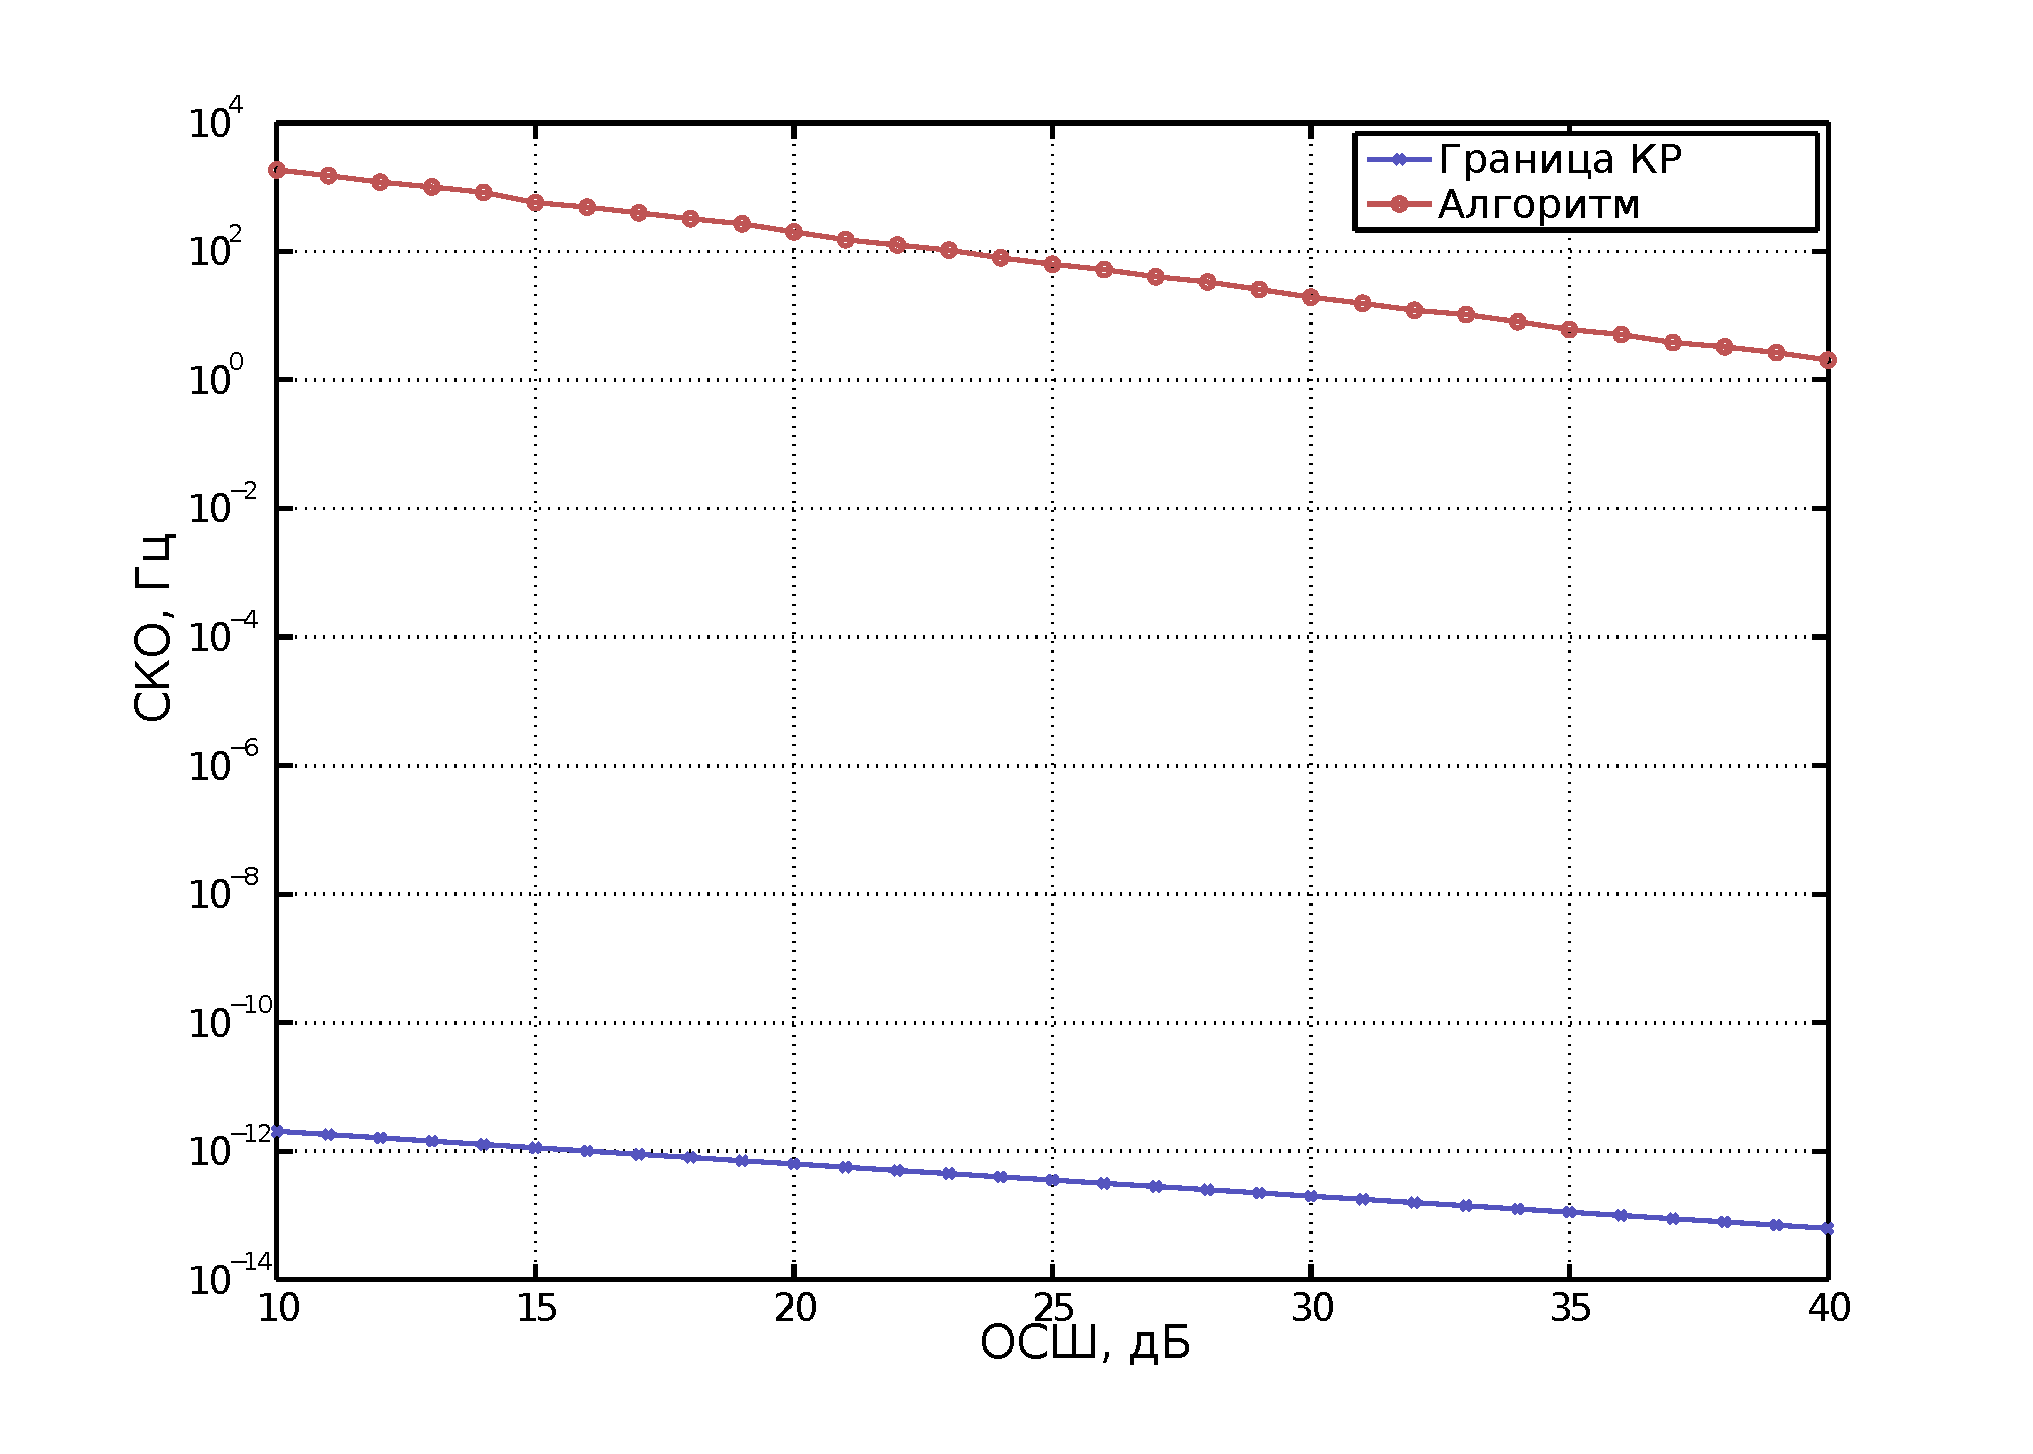
\includegraphics[width=1\linewidth]{crlb_vs_1sat_algo.eps}}
	\caption{СКО оценки частоты}
	\label{pic:crlb_vs_1sat_algo}
\end{figure}

Также в процессе математического моделирования была получена СКО оценки частоты при использовании алгоритма оценки информационных параметров для одного источника
сигнала в CDMA-системах на фоне АБГШ - \mbox{Рис. \ref{pic:crlb_vs_1sat_algo}}. Анализ результатов математического моделирования позволяет сделать  вывод о том,
что для сигналов с ОСШ не менее \mbox{25 дБ} можно получить оценку частоты с ошибкой не более \mbox{100 Гц}.

%%%%%%%%%%%%%%%%%%%%%%%%%%%%%%%%%%%%%%%%%%%%%%%%%%%%%%%%%%%%%%
\section{Выводы по Главе 1}

\begin{enumerate}
\item Задачу оценки информационных параметров ШПС СНС Navstar GPS с кодовым разделением каналов (CDMA) можно решить с помощью алгоритма на основе АР-модели,
	отличительной особенностью которого является сведение перебора в двумерной области неопределенности к перебору только по фазе ПСП и оценке
	резонансной частоты, повторно модулированного ПСП сигнала.

\item К достоинству данного алгоритма можно отнести то, что он позволяет снизить вычислительные затраты в 2 раза в сравнении с типовым подходом.
	Вычислительная сложность - общее количество умножений для оценки информационных параметров для одного источника сигнала в CDMA-системах на фоне АБГШ:
	${OP_{AR\_FOR\_1} = 24NlogN + 63N}$.

\item В предложенный алгоритм включена операция оценки оценки полюсов АР-модели, которая требует вычислений с плавающей точкой, а значит программно-аппаратная
	платформа должна иметь модуль для вычислений с плавающей точкой (в иностранной литературе floating point unit - FPU).

\item Результаты имитационного моделирования показали высокую чувствительность алгоритма к МКИ, что приводит к значительному смещению получаемых оценок
	частоты и мощности гармонического сигнала. Поэтому алгоритм на основе АР-модели требует усовершенствования.

\item В результате имитационного моделирование также была получено значение СКО точности оценки частоты. СКО оценки не превосходит \mbox{100 Гц} для сигналов
	с ОСШ более \mbox{25 дБ}.

%%%%%
%\item Разработан алгоритм на основе параметрического метода оценки информационных для одного источника с CDMA-сигналом на фоне аддитивного белого гауссового шума при отстутствии МКИ.
%	Получены значение вычислительной сложности и точности оценки частоты. Алгоритм на основе параметрического метода оценки частоты позволяет снизить вычислительные
%	затраты в 1.5 раза в сравнении с типовым подходом при этом точность оценки, при отсутствии МКИ, не превосходит нескольких десятков герц для сигналов
%	с ОСШ более 25 дБ.
%\item Вычислительная сложность - общее количество умножений для оценки частоты при помощи алгоритма оценки информационных параметров ШПС на фоне АБГШ c использованием \mbox{АР-модели}:
%	${OP_{AR\_FOR\_1} = 24NlogN + 63N}$.
%\item Оценка полюсов АР-модели требует вычислений с плавающей точкой, а значит программно-аппаратная платформа должна иметь модуль для вычислений с плавающей точкой
%	(в иностранной литературе floating point unit - FPU).
%\item Высокая чувствительность к МКИ - наличие окрашенного  шума приводит к значительному смещению получаемых оценок частоты и мощности гармонического сигнала.
\end{enumerate}

%%%%%%%%%%%%%%%%%%%%%%%%%%%%%%%%%%
%В реальных СПИ сигнал на приемник поступает одновременно от нескольких источников, присутствует неопределенность по частоте, а также аддитивный белый шум (АБГШ).
%В приемнике после оцифровки сигнала получаем смесь:
%\begin{equation}
%	\label{eq:cdma_strip_eq}
%	x(m)=\sum_{k=1}^{N}\left( A_k g(m + \tau_k)\exp{\left[j \left( \tilde{\omega}_{k}m + \phi_k(m)\right)\right]} \right) + n(m),
%\end{equation}
%где  ${k}$ - относительный номер источника сигнала, ${N}$ - количество доступных источников сигнала, модулированных ПСП одного семейства,
%${m}$ - индекс соответствующий времени, ${\tilde{\omega}_{k}}$  – относительная частота, соответствующая ${\omega_0}$,
%${\tau_k}$ - задержка модулирующей ПСП в точке приема, ${\phi_k(m)}$ - случайная начальная фаза, ${n(m)}$ - аддитивный белый гауссов шум (АБГШ). 
%
%Следует отметить, что при оценке фазы сигнала с номером ${k}$  интерференцией являются сигналы:    .
%\begin{equation}
%	%\label{eq:cdma_interference}
%	\{n \ne k, n \in [1,N]\}
%\end{equation}

%\subsection{Постановка задачи оценки параметров сигнала с расширенным спектром}
%\paragraph{Основные свойства широкополосных сигналов}
%
%%%%%%%
%\paragraph{Классическая постановка задачи оценки параметра.}
%
%%%%%%%
%%%%%%%
%\paragraph{Алгоритмы оценки параметров широкополосного сигнала сигнала.}
%
%%%%%%%%%
%% Chaos 
%Оценка параметров СПИ с ШПС (в частности сигналов системы Navstar GPS) с помощью осциллятора Дуффинга
%достаточно новое направление в исследованиях по данной тематике. В данной области опубликовано несколько работ, в частности \cite{chaos_chen, chaos_cambridge, chaos_huang, chaos_song}.
%Так же является интересной более ранняя статья не рассматривающая GPS \cite{chaos_wang}.
%Осциллятор Дуффинга с гармоническим внешним воздействием может быть описан уравнением:
%\begin{center}
%\begin{equation}
%	\label{eq:duffing}
%	mx'' + cx' + k_{1}x + k_{2}x^3 = F_{0}\cos(\omega{t}),
%\end{equation}
%\end{center}
%где $m$ - масса, $c$ - коэффициент диссипации, $x$ - состояние осциллятора, $k_1$ и $k_2$ - линейный и нелинейный коэффициенты соответственно,
%$F_{0}\cos(\omega{t})$ - внешнее воздействие.
%
%Подробно уравнение \ref{eq:duffing} рассмотрено в \cite{chaos_neimark_landa}.
%Для использования осциллятора Дуффинга с целью оценки параметров ШПС была предложена усовершенствованная форма \cite{chaos_song, chaos_chen}:
%\begin{center}
%\begin{equation}
%	\label{eq:duffing_gps}
%	x'' +cx' - x^3 + x^5 = \gamma\cos(\omega{t}) + (\gamma_{x}\cos(\omega_{x}) + n(t))
%\end{equation}
%\end{center}
%
%Перепишем динамическую систему \ref{eq:duffing_gps} в виде:
%\begin{center}
%\begin{equation}
%	\label{eq:duffing_gps_2}
%	\left\{
%	\begin{aligned}
%		y(t) & = x'(t) \\
%		y'(t) & =  -cx' + x^3 - x^5 + \gamma\cos(\omega{t}) + (\gamma_{x}\cos(\omega_{x}) + n(t)),
%	\end{aligned}
%	\right.
%\end{equation}
%\end{center}
%где ${n(t)}$ - АБГШ.
%
%Пример фазового портрета при ${\omega=\omega_{x}}$ изображен на рисунке \ref{pic:duffing_sync},
%фазовый портрет хаоса расположен на рисунках \ref{pic:duffing_chaos1}, \ref{pic:duffing_chaos2}
%\begin{figure}[H]
%	\center\scalebox{0.5}{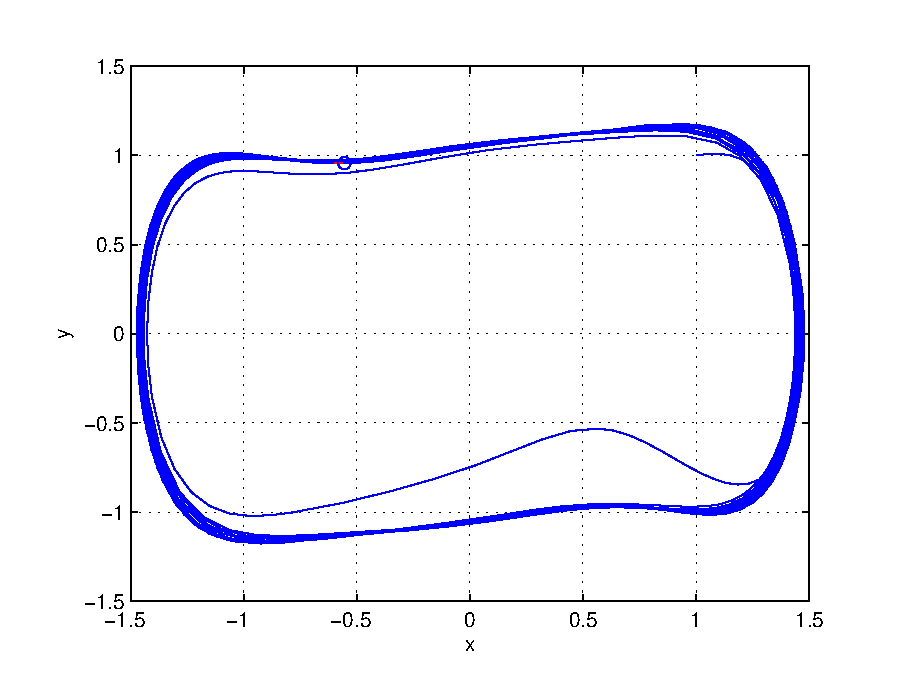
\includegraphics[width=1\linewidth]{duffing_sync.eps}}
%	\caption{Фазовый портрет при ${\omega =\omega_{x}}$}
%	\label{pic:duffing_sync}
%\end{figure}
%\begin{figure}[H]
%	\center\scalebox{0.5}{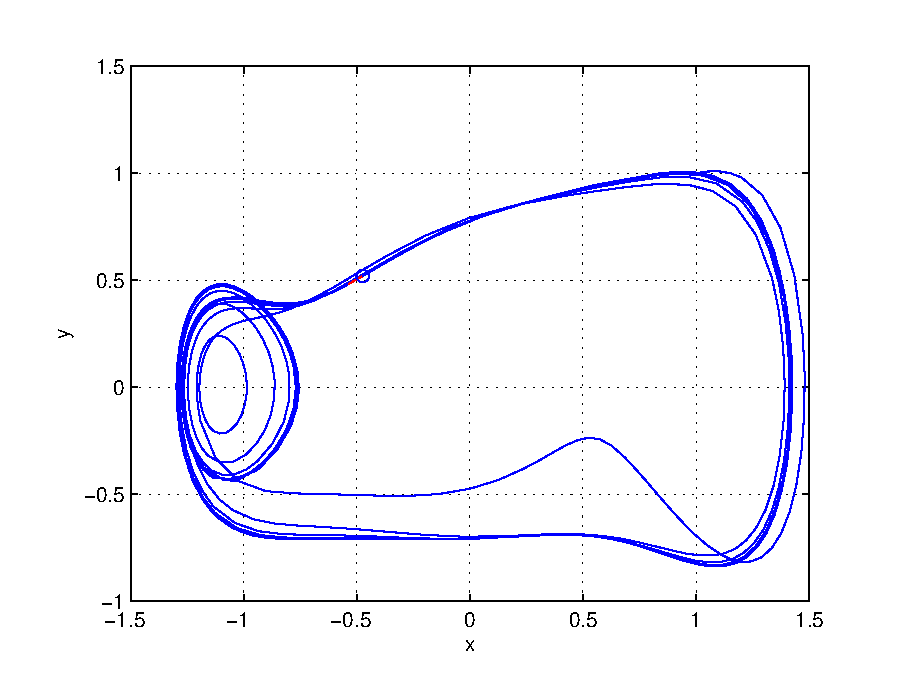
\includegraphics[width=1\linewidth]{duffing_chaos1.eps}}
%	\caption{Фазовый портрет при ${\omega < \omega_{x}}$}
%	\label{pic:duffing_chaos1}
%\end{figure}
%\begin{figure}[H]
%	\center\scalebox{0.5}{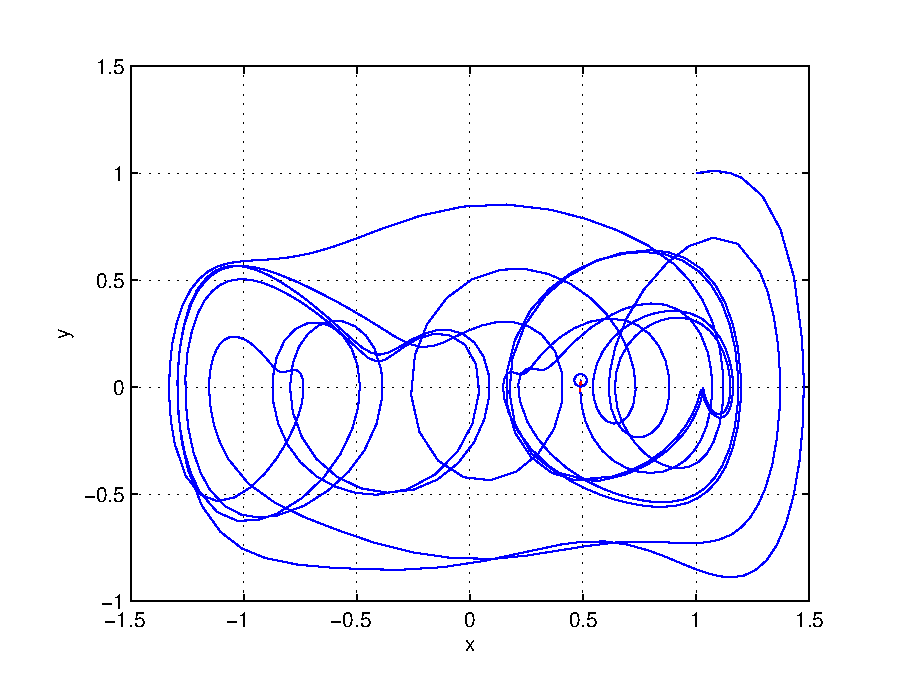
\includegraphics[width=1\linewidth]{duffing_chaos2.eps}}
%	\caption{Фазовый портрет при ${\omega > \omega_{x}}$}
%	\label{pic:duffing_chaos2}
%\end{figure}
%В качестве параметров уравнения применялись: $c = 0.5$, $\gamma=\gamma_{x}=0.36$, ${\omega=1}$
%
%Часто для вычисления характеристик хаотической динамики применяется показатель Ляпунова.
%Он показывает в каком состоянии находится система. Если система находится
%в стабильном состоянии линии фазовой траектории будут близко прилегать одна к другой, в противном
%случае система находится в состоянии хаоса. Детектор с применением показателя Ляпунова
%представлен на рисунке \ref{pic:chaos_lyapunov}.
%\begin{figure}[H]
%	\center\scalebox{0.7}{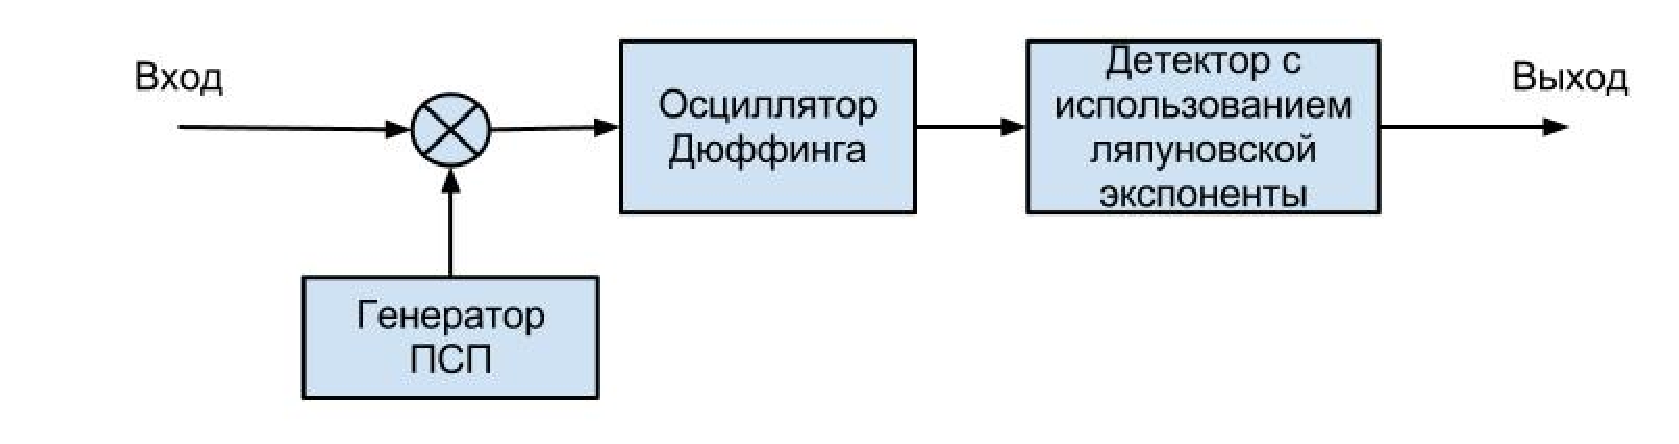
\includegraphics[width=1\linewidth]{Chaos_detector_Lyapunov.eps}}
%	\caption{Схема детектора основанного на показателе ляпунова для осциллятора Дуффинга}
%	\label{pic:chaos_lyapunov}
%\end{figure}
%
%В статье \cite{chaos_chen} предложен усовершенствованный метод, базирующийся на вычислении дисперсии
%фазовой траектории. Действительно, на рисунках \ref{pic:duffing_sync}, \ref{pic:duffing_chaos1},
%\ref{pic:duffing_chaos2} видно, что когда система находится в хаотическом состоянии значение
%дисперсии по координате ${x}$ больше, чем соответствующее значение в состоянии $\omega = \omega_{x}$.
%На основе этого была предложена усовершенствованная схема детектора сигнала - рисунок \ref{pic:chaos_energy_detector}
%\begin{figure}[H]
%	\center\scalebox{0.7}{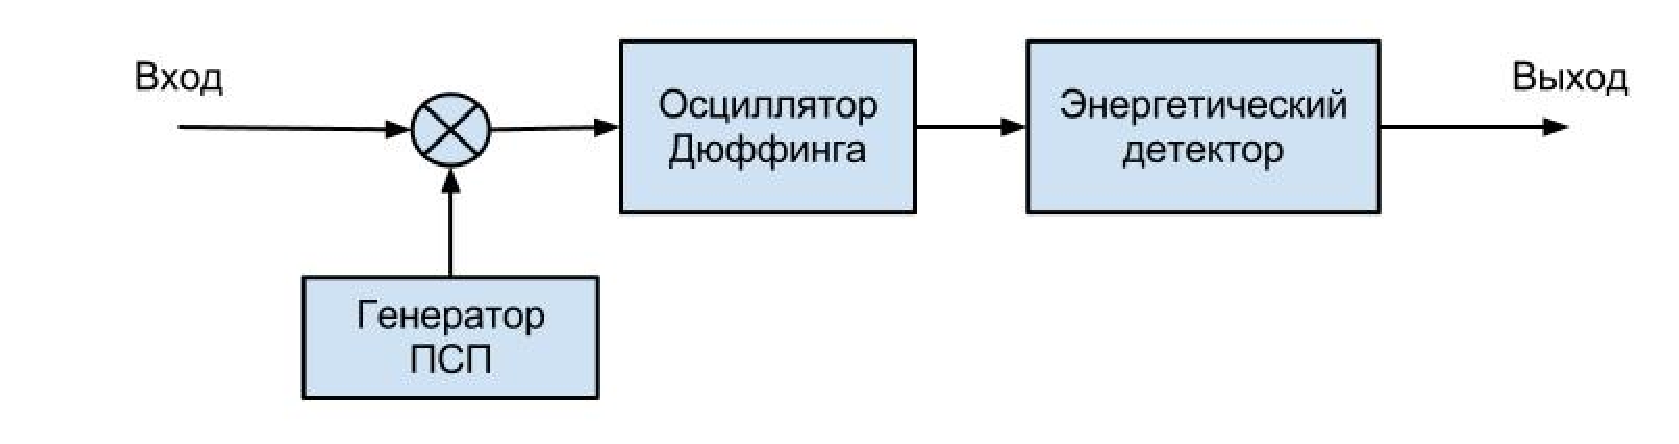
\includegraphics[width=1\linewidth]{chaos_detector.eps}}
%	\caption{Схема энергетического детектора для осциллятора Дуффинга}
%	\label{pic:chaos_energy_detector}
%\end{figure}
%
%%%%%%%%%
%% HOS 
%Математический аппарат статистик высоких порядков (СВП или HOS - Higher-order statistics)
%для исследования непричинных, причинных и нестабильных (систем с неминимальной фазой) и негауссовых сигналов впервые был предложен
%в \cite{hos_petropulu} в 1993 году.  Этот метод позволяет не только подавлять цветной Гауссов шум, но так же в некоторых случаях подавлять
%цветной не-Гауссов шум.
%
%В работе \cite{hos_zhao} был предложен метод детектирования ШПС с использованием СВП.
%
%%%%%%%%%
%% CHE 
%Интересная группа алгоритмов основывается на информационной избыточности ШПС, например \cite{phd_che}. В данной
%группе алгоритмов используется механизм появления нескольких точек на основном пике КФ, описанный в \cite{kaplan}. Пример
%изображен на рисунке \ref{pic:sec1_peak_tcd}.
%\begin{figure}[H]
%        \center\scalebox{1}{\includegraphics[width=1\linewidth]{corr_peak_tcd.eps}}
%        \caption{Идеальная КФ ШПС с отмеченными точками возможного обнаружения}
%        \label{pic:sec1_peak_tcd}
%\end{figure}
%На рисунке \ref{pic:sec1_peak_tcd} изображен пик КФ с несколькими точками. Две точки находятся выше порога ${\Pi=0.5}$.
%В работе \cite{phd_che} рассмотрено создание субоптимального обнаружителя на основе информационной избыточности ШПС.
%Получена целевая функция системы и намечены дальнейшие пути развития данного направления.
%
%%%%%%%%%
%% 2MAX 
%Так же одним из направлений исследований является разработка алгоритмов выбора порога без априорной информации о величине ОСШ. Например,
%в работах \cite{2max_ieee, 2max_article} представлен алгоритм нахождения пика (АНП) КФ (Peak-finding algorithm).
%
%Данный алгоритм можно разбить на несколько шагов:
%\begin{itemize}
%\item[Шаг 1] Подсчитать КФ, используя метод предложенный с использованием параллельного коррелятора. 
%\item[Шаг 2] Найти главный пик КФ, найти второй пик КФ, найти среднее значение КФ.
%\item[Шаг 3] Нормализовать полученные значения относительно главного пика КФ.
%\item[Шаг 4] Если (максимум КФ - среднее) > ${\Pi_1}$ и (максимум КФ - 
%	второй максимум КФ) > ${\Pi_2}$, тогда полученный главный пик КФ соответствует
%	искомой фазе ПСП и частоте.
%\end{itemize}
%
%В статье авторов \cite{2max_ieee} предложены следующие значения для порогов:
%${\Pi_1} = 0.3$ дБ и  ${\Pi_2} = 0.15$ дБ. Так же авторы предлагают итерационную процедуру для нахождения
%фазы ПСП и частоты смещения допплера:
%\begin{itemize}
%\item[Шаг 1] Начать вычисление с 1мс.
%\item[Шаг 2] Получить результаты АНП.
%\item[Шаг 3] Если фаза ПСП и частота не могут быть найдены, увеличить время интегрирования сигнала.
%	Использовать следующие значения для интегрирования: 1мс -> 10мс -> 50мс -> 100мс -> 200мс ->
%	500мс -> 1000мс
%\end{itemize}
%
%Очевидным минусом данного подхода является сильная зависимость от интерференции. В городском каньоне будет присутствовать
%несколько достаточно мощных лучей, а значит разница в энергии первого и второго пика будет низкой.
%
%%%%%%%
%\paragraph{Выводы.}
%
%Во введении кратко приведена история развития СПИ с ШПС, приведены ученые внесшие значительный вклад в разработку данного направления связи. Так же рассмотрена
%актуальность исследования в данной области. Кроме того, приведены определения, что такое СПИ с ШПС, ее математическая модель и основные отличительный особенности данного класса систем.
%Так же приведены классические и новые подходы к оценке параметров СПИ с ШПС. Рассмотрен оптимальный алгоритм - последовательный коррелятор,
%а так же новые достаточно экзотические подходы - применение осциллятора Дуффинга. 

\clearpage


\setcounter{chapter}{2}
\setcounter{section}{0}
\setcounter{equation}{0}
\setcounter{figure}{0}
\addcontentsline{toc}{chapter}{Глава 2. Усовершенствованный итеративный алгоритм вычисления оценки АКФ}
\chapter*{Глава 2. Усовершенствованный итеративный алгоритм вычисления оценки АКФ}
\label{l:sec_acf}

\section{Постановка задачи}

Для эффективного использования АР-метода необходимо иметь точную оценку АКФ. Наличие шума в аддитивной смеси ведет к неточной
оценке АКФ, что, в свою очередь, ведет к смещенной оценке резонансных частот. Вычислительная сложность итеративной оценки АКФ является квадратичной
функцией от длинны входной последовательности, поэтому итеративная оценка АКФ для нескольких источников не может быть реализована в программном приемнике
по причине большой ресурсоемкости. В данной главе ставится и решается задача оптимизации алгоритма итеративного вычисления АКФ. Также в данной
главе приводится обоснование возможности и эффективности применения итеративного алгоритма вычисления АКФ для подавления эффектов МКИ и повышения ОСШ сигнала
при оценке частоты в АР-модели. В конце главы представлено численное моделирование.

АКФ, по определению, представляет неслучайную функцию.
Для получения данной функции необходимо обладать бесконечным количеством реализаций или, в случае эргодического процесса, реализацией бесконечной длинны \cite{bolshakov-book}.

Оценка АКФ ${\hat{r}_{xx}(\tau, T)}$ является случайной функцией. Оценка данной функции должна наилучшим образом отражать реальные характеристики процесса.

Из большого числа методов оценки АКФ наиболее часто применяются прямые и косвенные. При использовании прямого метода вычисляется интеграл:
\begin{equation}
	\label{eq:acf_integral_basic}
	\hat{r}_{xx}(\tau, T) = \frac{1}{T-\tau} \int_{0}^{t-\tau} (x(t) - \hat{E}(x))(x(t+\tau) - \hat{E}(x))dt,
\end{equation}
где ${\hat{r}_{xx}(\tau, T)}$ -  оценка автокорреляционной функции. Остальные методы: основанные на интегральном преобразовании Фурье, использующие интеграл вероятностей, принцип
знакосочетаний, компенсации, интерференции, разложения по ортогональным функциям, относятся к косвенным \cite{bolshakov-book}.

Погрешности оценки можно разделить на три группы \cite{bolshakov-book}:
\begin{enumerate}
	\item Методические погрешности. Данные погрешности обусловлены ограниченностью отрезка реализации, шагом дискретизации и шумом квантования;
	\item Инструментальные погрешности. Данный вид погрешностей обусловлен погрешностями: измерительных приборов, записи, хранения, вычислений;
	\item Погрешности от влияния коррелированных и некоррелированных помех.
\end{enumerate}

Подходы к компенсации шума при АР анализе достаточно подробно рассмотрены в классических работах \cite{kay_ar_book, kay_noise_compensation}.
При наличии АБГШ во входной смеси ${x(m)}$ ее АКФ может быть записана как:
\begin{equation}
	\label{eq:acf_noise_basic}
	r_{xx}(m) =	\begin{cases}
				r_{ss}(0) + \sigma_n^2, & \mbox{если } m=0; \\
				r_{ss}(m), & \mbox{если } m \ne 0,
			\end{cases}
\end{equation}
где ${r_{ss}(m)}$ - АКФ гармонического сигнала 
Если вычесть ${\sigma_n^2}$ из ${r_{xx}(0)}$ в (\ref{eq:acf_noise_basic}) параметры АР процесса могут быть найдены. Однако, если ${\sigma_n^2}$ достаточно велика или 
оценка АКФ матрица входной смеси ${{\bf{\hat{R}_{xx}}}}$ плохая, матрица ${{\bf{\hat{R}_{xx}}} - {\bf{I}}\sigma_n^2}$ может быть не положительно определена. В данном
случае необходимо вводить поправочный коэффициент. Но для применения данного метода необходимы априорные знания или оценка ${\sigma_n^2}$,
что в случае оценки параметров ШПС в городских условиях (наличие интерференционной помехи от переотражения сигнала, а так же других источников сигнала,
наличие наличие преград на пути распространения сигнала и т.п.) является крайне затруднительным.

Различные методы оценки параметров для АР-модели, основанные на принципе максимального правдоподобия, не
могут считаться ММП при наличии шума в данных. В виду сложности использования ММП, в \cite{marpl_book, kay_ar_book} предложено несколько 
субоптимальных оценок:
\begin{enumerate}
	\item Применение АРСС;
	\item Фильтрация данных для уменьшения мощности шума;
	\item Компенсация параметров АР или оценки коэффициентов отражения;
	\item Использования АР-модели более высокого порядка.
\end{enumerate}

Разрешающая способность оценки частоты при применении АР-модели снижается при снижении уровня ОСШ.
Разрешающую способность оценки АР-модели для гармонических сигналов
одинаковой мощности в случае известной АКФ можно определить приблизительно с помощью формулы Марпла \cite{marpl_book, kay_ar_book}:
\begin{equation}
	\label{eq:lpc_est_quality_1}
	F = \frac{1.03}{Tp[R_e(P+1)]^{0.31}},
\end{equation}
где ${F}$ - разрешение в герцах, ${T}$ - интервал отсчетов в секундах, ${P}$ - порядок модели, ${R_e}$ - ОСШ для отдельного гармонического сигнала, выраженный в линейных единицах.

В работах \cite{lacoss_spectral_est, chen_spectral_est, marple_1977} предложены способы повышения разрешающей способности в задаче оценки спектра входной смеси, но
в данных работах не рассмотрен еще один интересный алгоритм уточнения АКФ - итеративный пересчет АКФ \cite{ostanin_akf}. В данной работе используется
модификация данного алгоритма поэтому целесообразно рассмотреть его подробнее.

В \cite{ostanin_akf} предлагается использовать метод последовательного вычисления АКФ для уточнения оценки АКФ. Данный метод
заключается в последовательном вычислении АКФ от АКФ несколько раз. При этом ОСШ увеличивается от итерации к итерации.
Процесс повторяется несколько раз. Количество итераций зависит от значения ОСШ сигнала. Возможность применения данного подхода в оценке параметров ШПС рассмотрена
автором в \cite{my_acf_cdma}.

%%%%%%%%%%%
\section{Алгоритм итеративного вычисления АКФ}
\label{sec_ostanin}

Пусть входная смесь может быть записана как сумма полезного сигнала ${s(t)}$ и шума ${n(t)}$:
\begin{equation}
	\label{eq:acf_signal}
	x(t) = A \cos{(\omega t)} + n(t)
\end{equation}

Пусть функции ${s(t)}$ и ${n(t)}$ - центрированы. Тогда АКФ выражения (\ref{eq:acf_signal}) может быть записана как \cite{book_max}:
\begin{eqnarray}
	\label{eq:acf_rss_signal}
	r_{xx}(\tau)	& = & \lim_{T \to \infty} \frac{1}{T} \int \limits_0^T x(t)x(t-\tau)dt = \nonumber \\
			& = & \lim_{T \to \infty} \frac{1}{T} \int \limits_0^T (A \cos{(\omega t)} + n(t))(A \cos{(\omega t - \tau)}) + \\
			&   & + n(t - \tau))dt \nonumber
\end{eqnarray}

Тогда, оценка АКФ может быть записана как:
\begin{equation}
	\label{eq:acf_rss_signal_full}
	\hat{r}_{xx}(\tau)=\hat{r}_{ss}(\tau)+\hat{r}_{sn}(\tau)+\hat{r}_{ns}(\tau) + \hat{r}_{nn}(\tau).
\end{equation}

Корреляционные функции ${\hat{r}_{sn}}$ и ${\hat{r}_{ns}}$ тождественно равны 0, с точностью до погрешности, при условии независимости
${x(t)}$ и ${n(t)}$. Таким образом (\ref{eq:acf_signal}) можно переписать:
\begin{equation}
	\label{eq:acf_rss_signal_new}
	\hat{r}_{xx}(t) = \hat{r}_{ss}(t) + \epsilon (t)
\end{equation}

Стоит учесть, что ${\epsilon (t)}$ стремится к нулю с ростом ${T}$. Фурье-образ ${\hat{r}_{xx}(t)}$
представляет собой СПМ, а, следовательно, равен квадрату Фурье-образа исходной функции ${x(t)}$.
Если обозначить ОСШ, выраженное в линейных единицах, сигнала ${x(t)}$ как ${R_s}$, тогда ОСШ после вычисления АКФ может быть выражено 
как \cite{book_max}:
\begin{equation}
	\label{eq:acf_snr_est}
	R_e=2BTR_s \frac{1}{2+1/R_s},
\end{equation}
где ${B}$ - эффективная полоса частот, ${T}$ - длительность, а ${R_s}$ - ОСШ сигнала.

Стоит отметить, что функция ${\epsilon(\tau)}$, как и ${n(t)}$ - является центрированной и
стационарной случайной величиной.
Учитывая, что гармоническая составляющая содержится в ${\hat{r}_{ss}(t)}$, а аддитивный шум в ${\epsilon(\tau)}$, можно провести
следующую итерацию вычисления АКФ. Для оценки ОСШ по формуле (\ref{eq:acf_snr_est}) нужно принять ${R_s' = R_e}$.

Из (\ref{eq:acf_snr_est}) видно, что увеличение ОСШ при вычислении оценки АКФ пропорционально ${2BT}$ и зависит от
ОСШ на входе коррелометра, также можно отметить, что увеличение ОСШ происходит только при условии ${BT > \frac{1}{2R_s} + 1}$.
Оценка прироста ОСШ на ${k}$-ой итерации получается рекуррентно по формуле (\ref{eq:acf_snr_est}).

На Рис. \ref{pic:acf_0_iter} представлен входной сигнал, а на
Рис. \ref{pic:acf_1_iter}, \ref{pic:acf_4_iter} представлены оценки АКФ на первом и четвертом шагах.
Моделирование проводилось для гармонического сигнала при ОСШ -43.82 дБ с нормированной частотой 20 Гц для
отрезка 600 точек.

\begin{figure}[h]
	\center\scalebox{1}{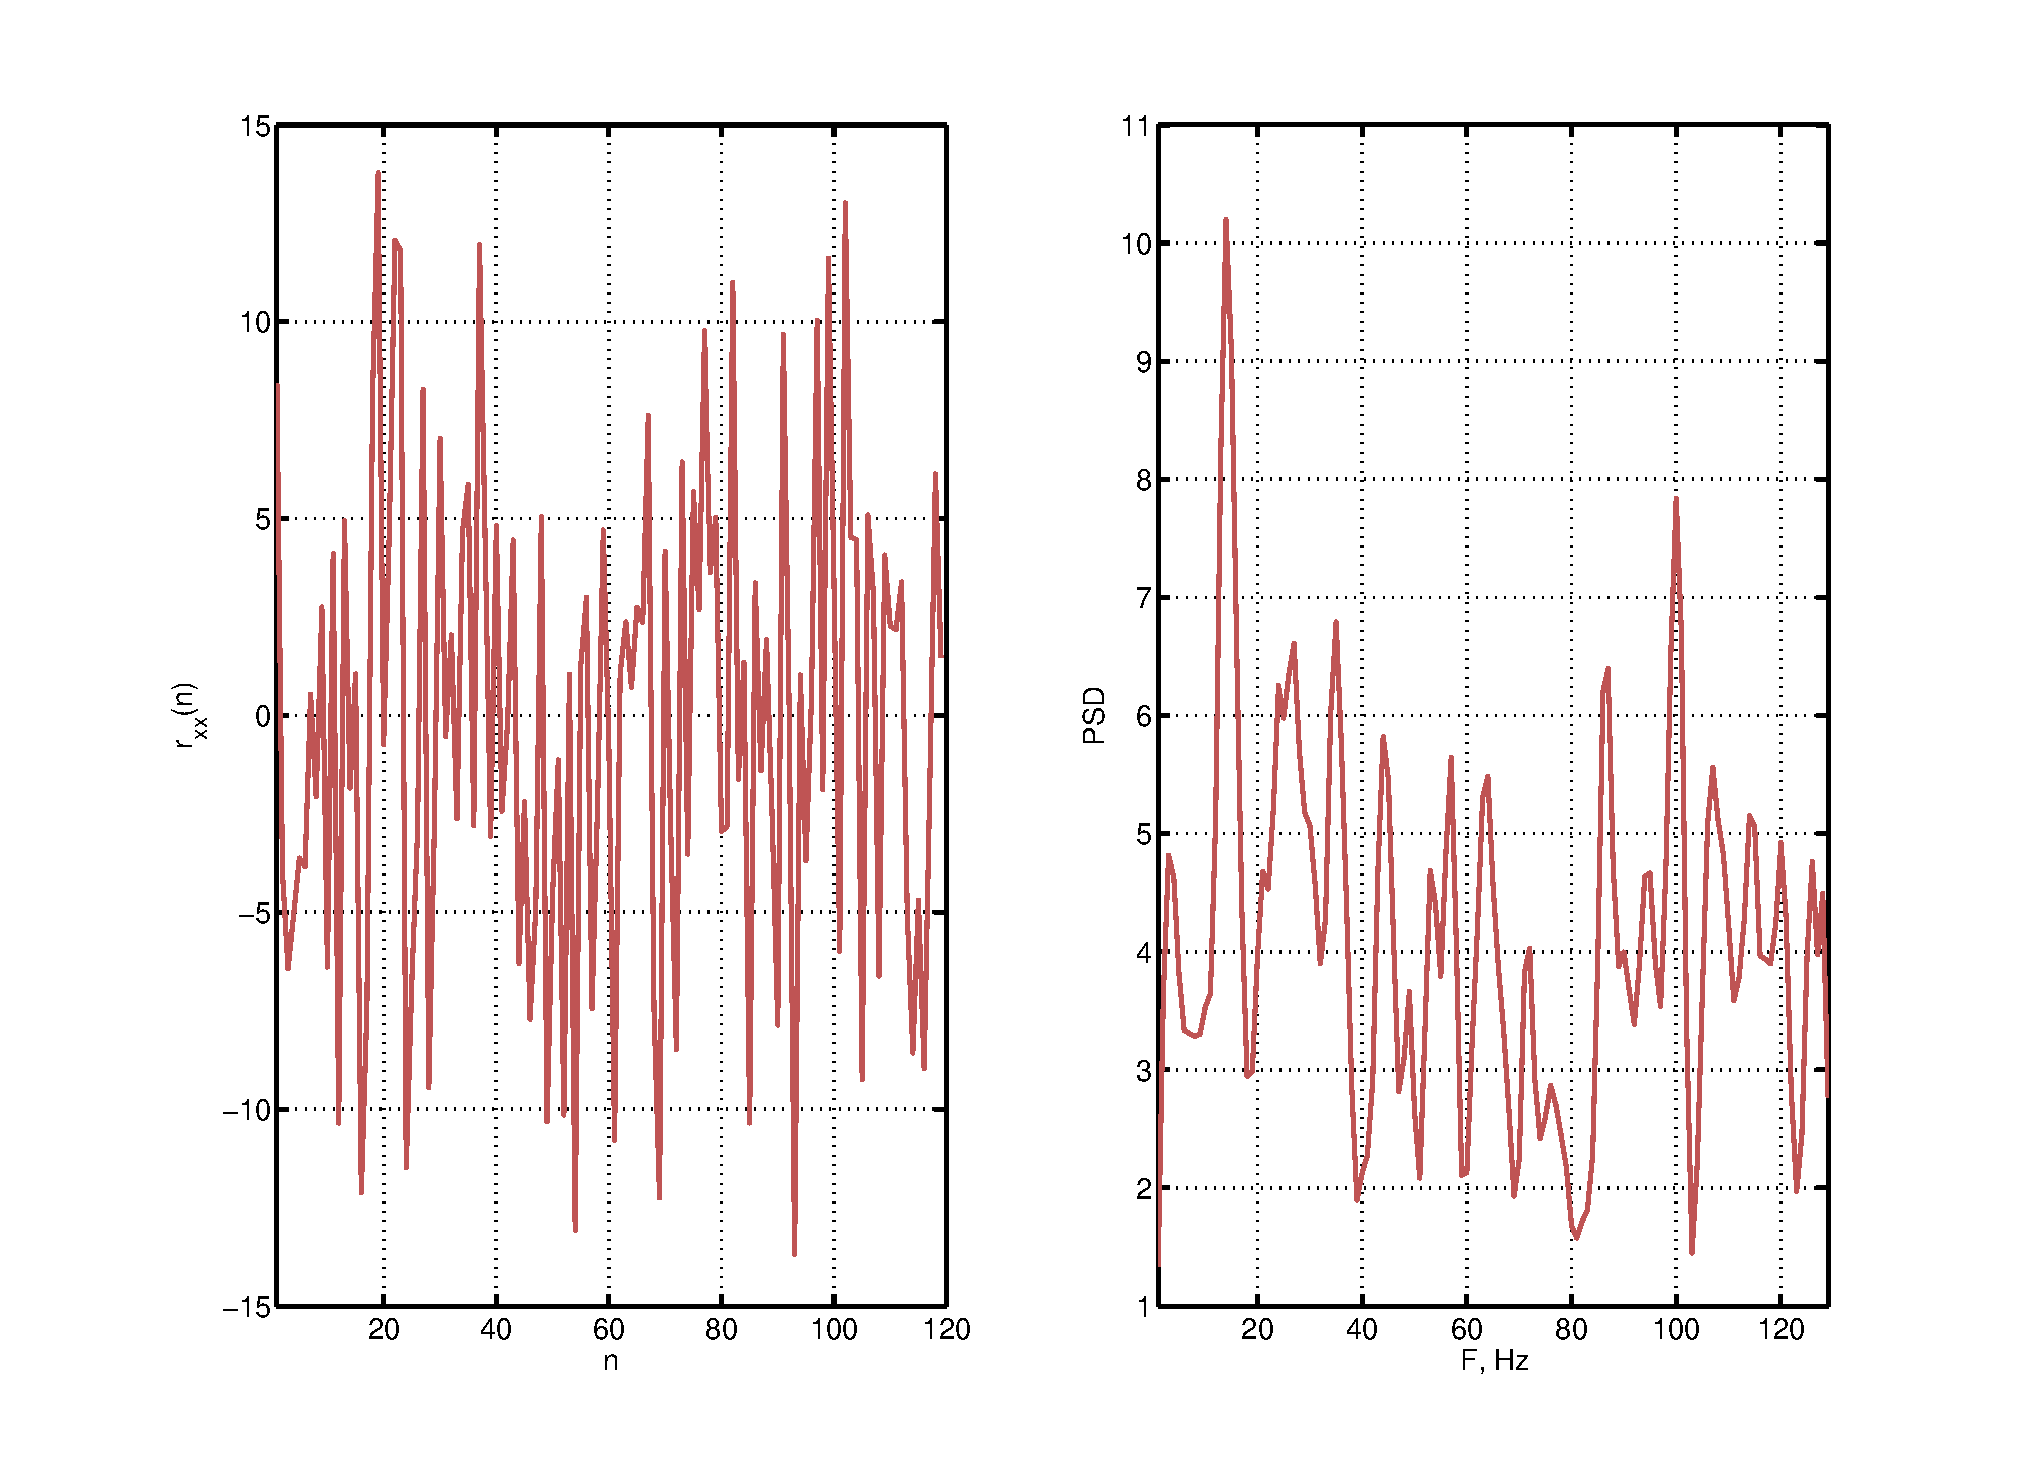
\includegraphics[width=1\linewidth]{acf_0_iter.eps}}
	\caption{Исходный сигнал и его спектр.}
	\label{pic:acf_0_iter}
\end{figure}

\begin{figure}[h]
	\center\scalebox{1}{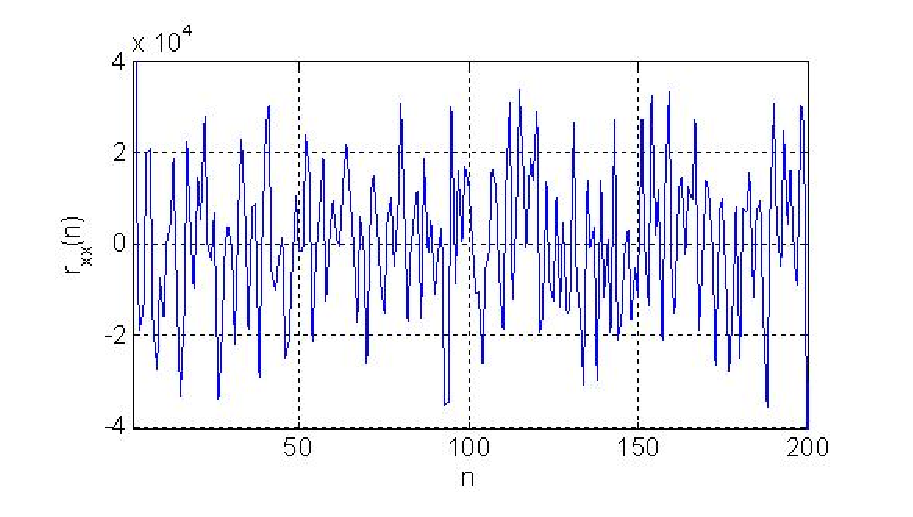
\includegraphics[width=1\linewidth]{acf_1_iter.eps}}
	\caption{Оценка АКФ на 1 итерации и ее спектр.}
	\label{pic:acf_1_iter}
\end{figure}

\begin{figure}[h]
	\center\scalebox{1}{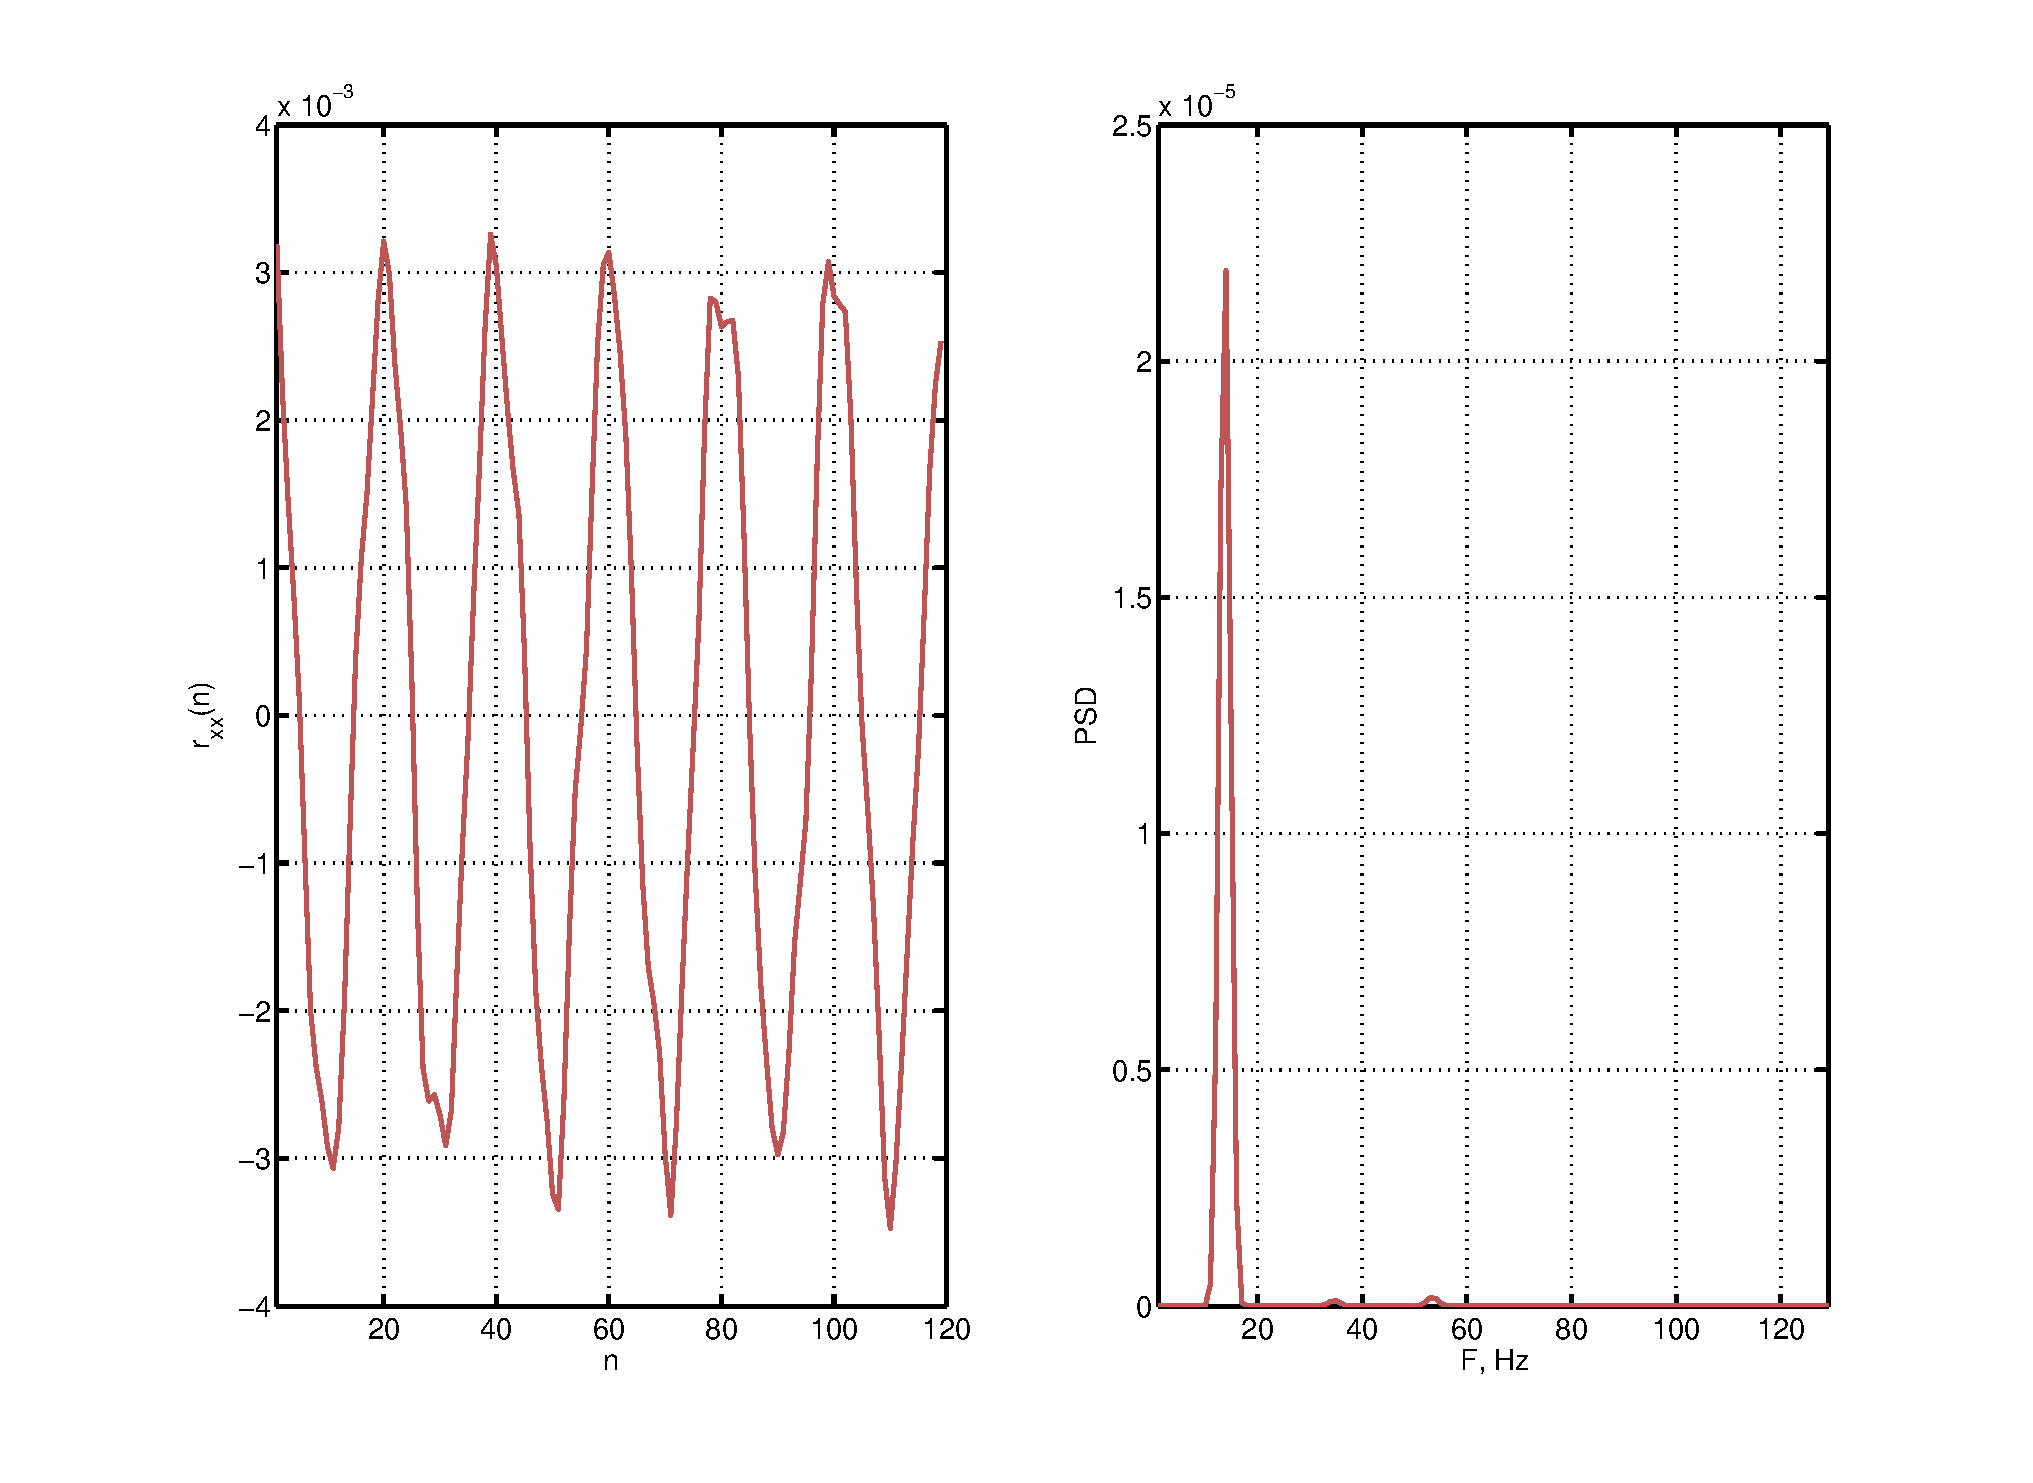
\includegraphics[width=1\linewidth]{acf_4_iter.eps}}
	\caption{Оценка АКФ на 4 итерации и ее спектр.}
	\label{pic:acf_4_iter}
\end{figure}

Представленный алгоритм позволяет значительно улучшить оценку АКФ. Следует отметить, что итеративный алгоритм вычисления АКФ так же
может быть использован для эффективного подавления окрашенного шума. В случае наличия интерференционной помехи в сигнале это дает
возможность получить несмещенную оценку частоты.

%%%%%%%%%%%%%%%%%
\section{Усовершенствованный итеративный алгоритм получения АКФ}
\label{sec_acf_fft}
Для приемников реального времени алгоритм, представленный в \cite{ostanin_akf} и приведенный в (\ref{sec_ostanin}), применять при оценке 
частоты ШПС не представляется возможным ввиду большого количества операций при вычислении АКФ.

Автором в \cite{my_acf} был предложен способ оптимизации алгоритма последовательного вычисления АКФ.
Для снижения вычислительных затрат указанный алгоритм предлагается реализовывать с использованием процедуры БПФ. 

Посчитаем АКФ для выражения (\ref{eq:acf_signal}).
\begin{equation}
	\label{eq:lpc_akf_n}
	\hat{r}_{xx}(n) = \sum \limits_{k=1}^{K} x(k)x(k+n) = \frac{A^2}{2} \cos{(\omega{n})} + \Delta_n \delta{(n)} + \mu{(n)}
\end{equation}

Здесь ${\Delta_n}$ - дисперсия шума ${n(k)}$, ${\mu{(n)}}$ - ошибка оценки АКФ, ${\delta{(n)}}$ - дельта-функция. Дисперсия ошибки
оценки ${\Delta_{\mu}}$ будет в ${K}$-раз меньше чем дисперсия ${\Delta_n}$ шума в принимаемом сигнале, где ${K}$ - интервал
осреднения оценки АКФ.

Используя оценку АКФ вместо исходной выборки, вновь получим оценку АКФ:
${r_{xx2}(n) = \frac{A^4}{8} \cos{(\omega n)} + \bar{N} \delta{(N)}}$,
где мощность шума оценки ${\bar{N}}$ - будет значительно меньше.

Амплитуда сигнала на итерации ${k}$ будет равна ${\frac{A^{2^k}}{2^{2^k-1}}}$. Увеличение отношения ОСШ по мощности можно
вычислить по уже приведенной формуле (\ref{eq:acf_snr_est}). 

Таким образом алгоритм можно представить в следующем виде.

Введем следующие обозначения: ${\bf{x}}$ – вектор входной смеси после повторной модуляции с ПСП, ${\bf{F}}$ – матрица прямого преобразования Фурье,
${\bf{F}^{-1}}$- матрица обратного преобразования Фурье.  Оценку АКФ на первом шаге можно получить следующим образом:
\begin{equation}
	\label{eq:akf_1}
	\hat{\bf{r}}_1 = \bf{F}^{-1}\left[ \bf{Fx} \cdot (\bf{Fx})^* \right] = \bf{F}^{-1} \left[ \left| \bf{Fx} \right| ^2 \right].
\end{equation}

Здесь знак ${(\cdot)}$  означает поэлементное перемножение векторов, ${\left| \bf{Fx} \right| ^2}$ - поэлементное возведение модуля комплексного числа в квадрат, ${*}$ -
комплексное сопряжение.  Следуя алгоритму, изложенному в \cite{ostanin_akf} вычислим оценку АКФ от ${\hat{\bf{r}}_1}$:
\begin{eqnarray}
	\label{eq:akf_2}
	\hat{\bf{r}}_2 & = & \bf{F}^{-1}\left[ \bf{F} \hat{\bf{r}}_1 \cdot (\bf{F} \hat{\bf{r}}_1)^* \right] = \nonumber \\
		& = & \bf{F}^{-1}	\left[ 
				\bf{FF}^{-1} \left[
						\left| \bf{Fx} \right| ^2
					\right]
						\cdot \left( \bf{FF}^{-1} \left[ \left| \bf{Fx} \right| ^2 \right]
					\right) ^*
			\right] = \nonumber \\
		& = & \bf{F}^{-1} \left[ \left| \bf{Fx} \right| ^2 \cdot \left[ \left| \bf{Fx} \right| ^2 \right] ^* \right] =  \nonumber \\
		& = & \bf{F}^{-1} \left[ \left| \bf{Fx} \right| ^4 \right].
\end{eqnarray}

Таким образом, уточненная оценка АКФ на ${K}$-ом шаге алгоритма, рассмотренного в \cite{ostanin_akf}
может быть получена без использования итераций с помощью выражения:
\begin{equation}
	\label{eq:akf_3}
	\hat{\bf{r}}_K = \bf{F}^{-1}\left[ \left| \bf{Fx} \right| ^{2^K} \right].
\end{equation}

Схематически алгоритм вычисления уточненной оценки АКФ на третьем шаге представлен на Рис. \ref{pic:akf_pic}.

\begin{figure}[h]
	\center\scalebox{0.8}{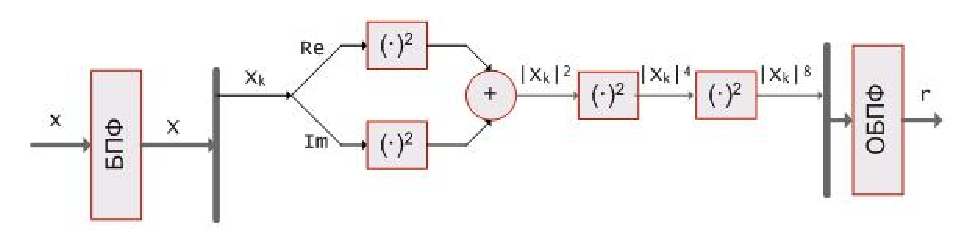
\includegraphics[width=1\linewidth]{akf_fft.eps}}
	\caption{Усовершенствованный итеративный алгоритм получения АКФ}
	\label{pic:akf_pic}
\end{figure}

Количество умножений действительных чисел, необходимых для оценки АКФ прямым методом без применения БПФ: 
\begin{equation}
	\label{eq:num_of_op_acf}
	OP_{ACF}=kN^2,
\end{equation}
где ${k}$  – количество итераций.

Количество умножений действительных чисел для получения оценки АКФ с применением усовершенствованного алгоритма вычисления оценки АКФ:
\begin{enumerate}
\item ${4NlogN}$ - действительных умножений - преобразование Фурье;
\item ${2N}$ - вычисление модуля комплексного числа;
\item ${N}$ - действительных умножений для каждой итерации (возведение в квадрат);
\item ${4NlogN}$ - действительных умножений – обратное преобразование Фурье. 
\end{enumerate}

Окончательно получаем:
\begin{equation}
	\label{eq:num_of_op_acf}
	OP_{ACF\_FFT}=8NlogN + (k+2)N.
\end{equation}

\section{Применение оконного взвешивания для оценки СПМ}

Так как в реальных условиях присутствует неопределенность по частоте, а длинна анализируемого объема данных конечна, пик на ПЧ в спектральной области не будет
представлять дельта функцию. Для улучшения свойств оценки СПМ представляется возможным использовать функции окон ${w(n)}$ - операция оконного взвешивания.
Свойства различных окон подробно рассмотрены, например, в \cite{shahtarin-spectrum-book, bolshakov-book}.

Наиболее популярными окнами являются: прямоугольное (равномерное), Бартлетта (треугольное), Ханна (косинус-квадрат), Хемминга (приподнятый косинус).

Оконная функция симметричного прямоугольного окна(\mbox{Рис. \ref{pic:win_rect}}) представляется выражением:
\begin{equation}
	\label{eq:rect_window}
	 w(n) = \begin{cases}
		1, |n| \le M; \\
		0, \mbox{в остальных случаях}.
		\end{cases}
\end{equation}
\begin{figure}[h]
	\center\scalebox{1}{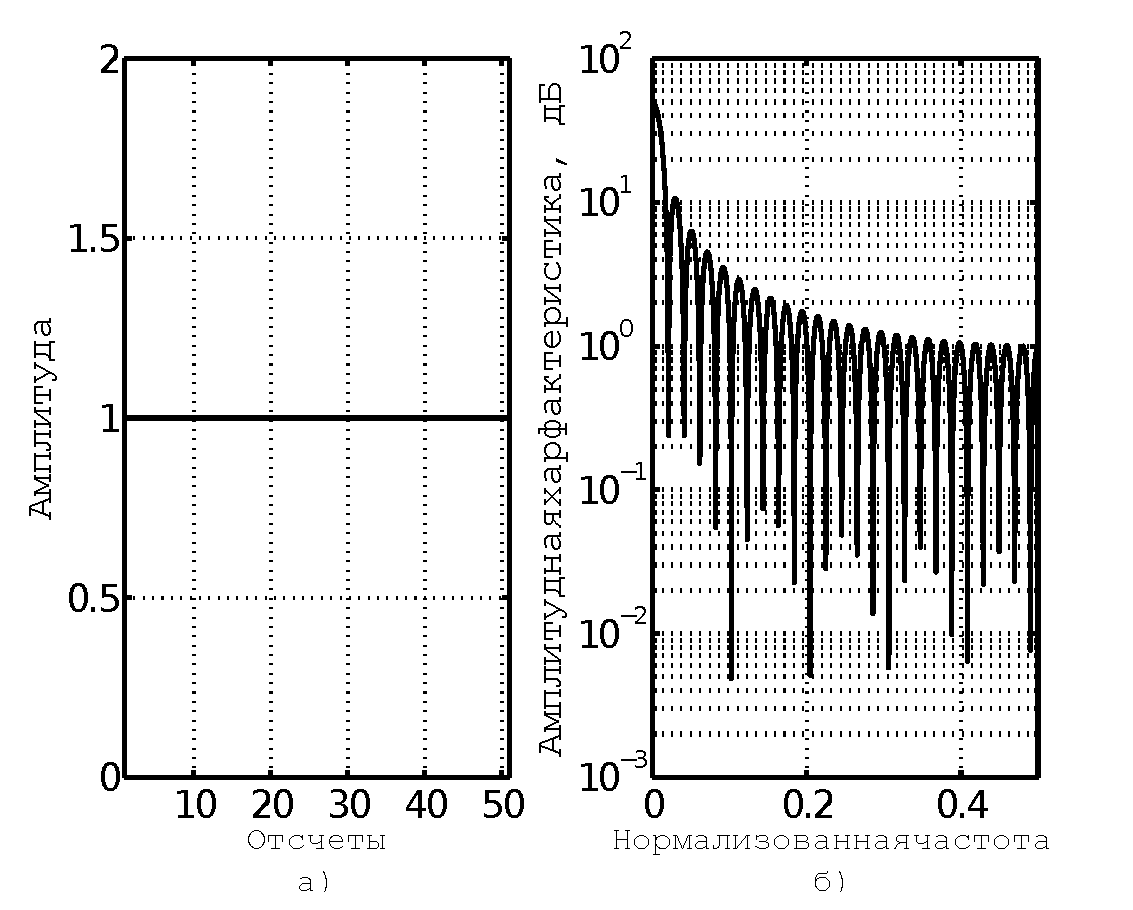
\includegraphics[width=1\linewidth]{various_windows_fig4.eps}}
	\caption{Прямоугольное окно. а - во временной области, б - в частотной}
	\label{pic:win_rect}
\end{figure}

Окно Бартлетта (\mbox{Рис. \ref{pic:win_bart}}) может быть представлено выражением:
\begin{equation}
	\label{eq:rect_bartlett}
	 w(n) = \begin{cases}
		1 - \frac{|n|}{M}, |n| \le M; \\
		0, \mbox{в остальных случаях}.
		\end{cases}
\end{equation}
\begin{figure}[h]
	\center\scalebox{1}{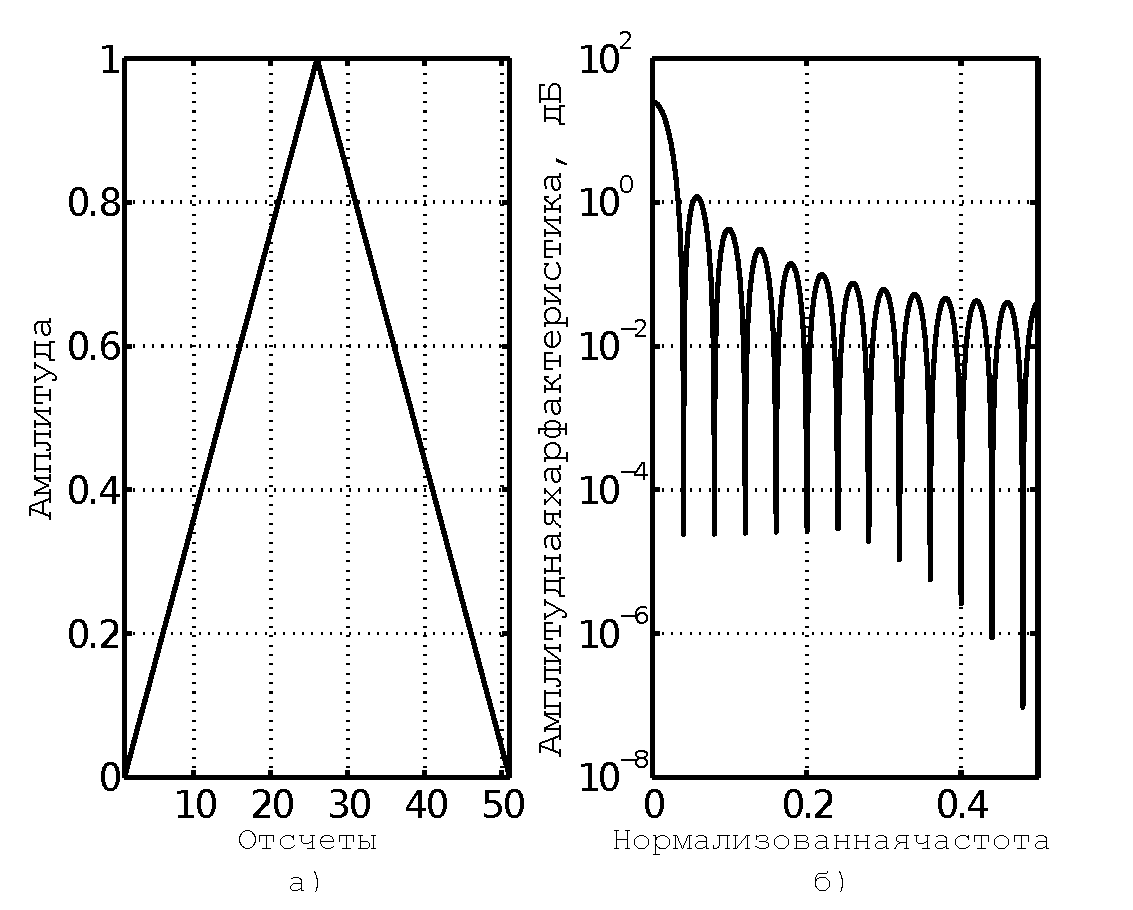
\includegraphics[width=1\linewidth]{various_windows_fig3.eps}}
	\caption{Окно Бартлетта. а - во временной области, б - в частотной}
	\label{pic:win_bart}
\end{figure}

Окно Хемминга (\mbox{Рис. \ref{pic:win_hamming}}) может быть представлено выражением:
\begin{equation}
	\label{eq:rect_hamming}
	 w(n) = \begin{cases}
		0.54 - 0.46\cos \left( 2 \pi \frac{n}{M} \right), 0 \le n \le M; \\
		0, \mbox{в остальных случаях}.
		\end{cases}
\end{equation}
\begin{figure}[h]
	\center\scalebox{1}{\includegraphics[width=1\linewidth]{various_windows_fig2.eps}}
	\caption{Окно Хемминга. а - во временной области, б - в частотной}
	\label{pic:win_hamming}
\end{figure}

Окно Ханна (\mbox{Рис. \ref{pic:win_hann}}) может быть представлено выражением:
\begin{equation}
	\label{eq:rect_hann}
	 w(n) = \begin{cases}
		0.5 \left( 1 - \cos\left( 2 \pi \frac{n}{M} \right) \right) \\
		0, \mbox{в остальных случаях}.
		\end{cases}
\end{equation}
\begin{figure}[h]
	\center\scalebox{1}{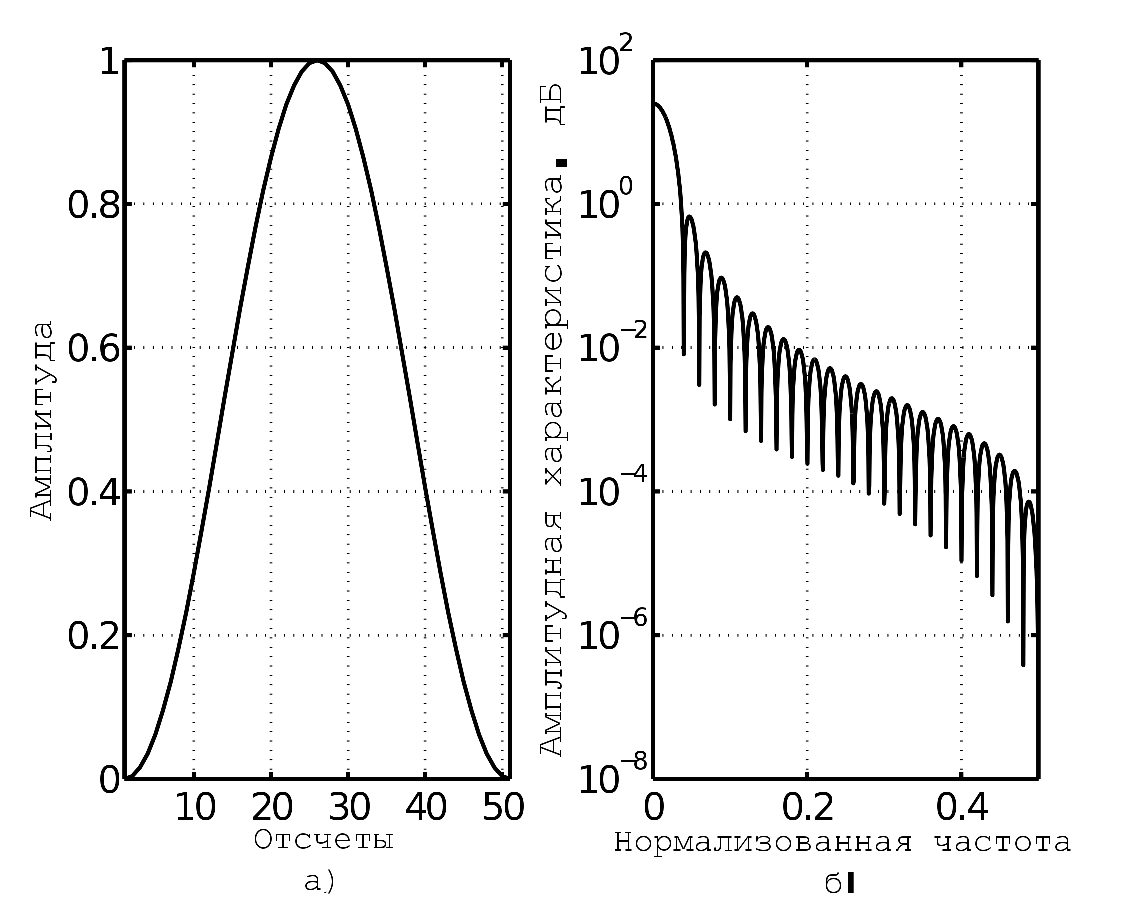
\includegraphics[width=1\linewidth]{various_windows_fig1.eps}}
	\caption{Окно Ханна. а - во временной области, б - в частотной}
	\label{pic:win_hann}
\end{figure}

Основными недостатками прямоугольного окна являются: наличие ложных максимумов, знакопеременность. В тоже время прямоугольное окно имеет самую малую ширину главного лепестка, но
одновременно с этим достаточно большие и медленно убывающие знакопеременные боковые лепестки. Окна Бартлетта и Ханна всюду положительны, а окно Хемминга положительно не всюду, однако
первый боковой лепесток составляет 0.021 высоты основного лепестка. Этим обусловлена популярность данного окна в задачах спектрального анализа.

В виду того, что задача итеративной оценки АКФ не является стандартной задачей спектрального анализа необходимо провести дополнительные исследования. В процессе
диссертационной работы было проведено численное моделирование применения разных окон в алгоритме итеративного вычисления оценки АКФ.

{\bf{\textit{Применение оконного взвешивания в задаче итеративного вычисления АКФ}}}

Из \cite{bolshakov-book} известно, что прямоугольное окно является самым узким, но вместе с тем имеет достаточно существенные боковые лепестки. В задаче итеративной оценки
АКФ, функция умножается несколько раз поточечно в частотном домене. Это позволяет предположить, что боковые лепестки будут увеличивать свое значение медленнее основного.
Для проверки данной гипотезы был проведен вычислительный эксперимент.

%%%%%%
\section{Практические аспекты применения}
\label{lab:sec2_windows}

При практической реализации алгоритма оценки частоты на основе АР-модели важным является качество оценки АКФ функции. В предложенном алгоритме итеративной оценки АКФ,
в случае блочной обработки данных, будет наблюдаться эффект растекания спектра вследствии того, что ПЧ не является кратной частоте дискретизации. В процессе диссертационного
исследования было проведено численное моделирование применения различных комбинаций оконных функций и различных длин блоков нулей, при вычислении БПФ для повышения
разрешающей способности, как это рекомендовано для алгоритмов оценки СПМ \cite{bolshakov-book}.

В \cite{bolshakov-book} отмечено, что для повышения разрешения в методах, основанных на корреляционных функциях, можно дополнять исходную последовательность нулями.
Но, с другой стороны, при добавлении нулей ко входной последовательности количество операций для оценки АКФ возрастает. Таким образом необходимо провести дополнительное
исследование для оценки минимально возможного количества нулей, которые необходимо добавить ко входной последовательности для повышения точности оценки частоты,
удовлетворяющей входной расстройке ФАПЧ.

Для оценки количества нулей, необходимых для попадания оценки частоты в диапазон допустимой входной расстройки ФАПЧ был проведен вычислительный эксперимент. В качестве диапазона
ОСШ был взят диапазон от -30 дБ до 5 дБ, количество нулей в диапазоне ${[0, 6N]}$, где ${N}$ - длинна данных. Допустимая входная расстройка была взята в диапазоне ${[-40, 40]}$ Гц.
Опыт проводился на фоне АБГШ без МКИ. Оценивалось СКО оценки при использовании разных типов окон и разного количества итераций пересчета АКФ.

На Рис. \ref{pic:fft2_1} представлено моделирование для последовательности дополненной нулями до длинны ${2N}$ с применением различных оконных функций:
прямоугольного окна, окна Хемминга, окна Блекмана и окна Ханна при одной итерации уточнения АКФ.
\begin{figure}[h]
	\center\scalebox{0.8}{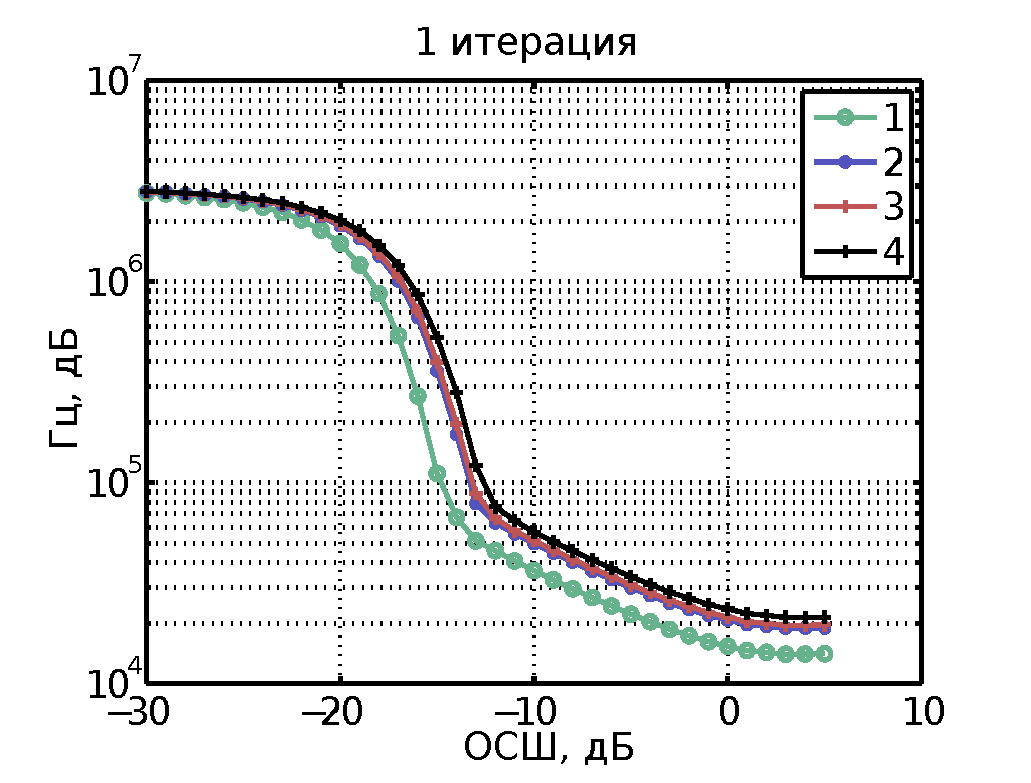
\includegraphics[width=1\linewidth]{fft2_1.eps}}
	\caption{СКО оценки частоты.\\1 - прямоугольное окно, 2 - окно Хемминга, 3 - окно Блекмана, 4 - окно Ханна.}
	\label{pic:fft2_1}
\end{figure}

На Рис. \ref{pic:fft2_2} представлено моделирование для последовательности дополненной нулями до длинны ${2N}$ с применением различных оконных функций:
прямоугольного окна, окна Хемминга, окна Блекмана и окна Ханна при двух итерациях уточнения АКФ.
\begin{figure}[h]
	\center\scalebox{0.8}{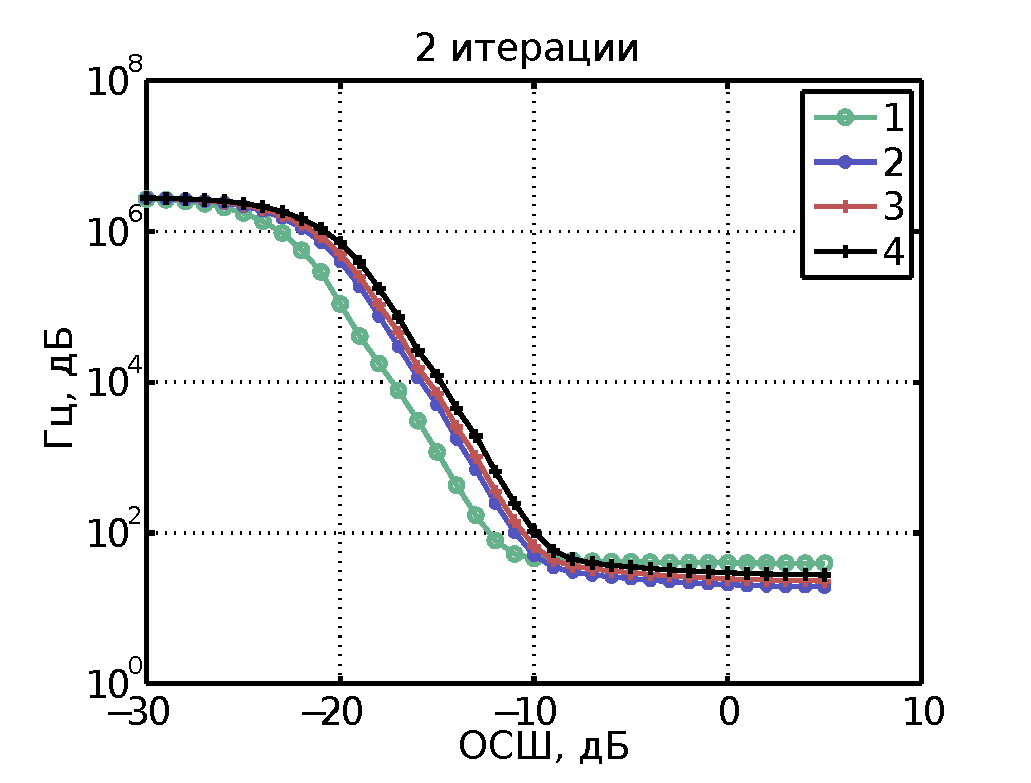
\includegraphics[width=1\linewidth]{fft2_2.eps}}
	\caption{СКО оценки частоты.\\1 - прямоугольное окно, 2 - окно Хемминга, 3 - окно Блекмана, 4 - окно Ханна.}
	\label{pic:fft2_2}
\end{figure}

На Рис. \ref{pic:fft2_3} представлено моделирование для последовательности дополненной нулями до длинны ${2N}$ с применением различных оконных функций:
прямоугольного окна, окна Хемминга, окна Блекмана и окна Ханна при трех итерациях уточнения АКФ.
\begin{figure}[h]
	\center\scalebox{0.8}{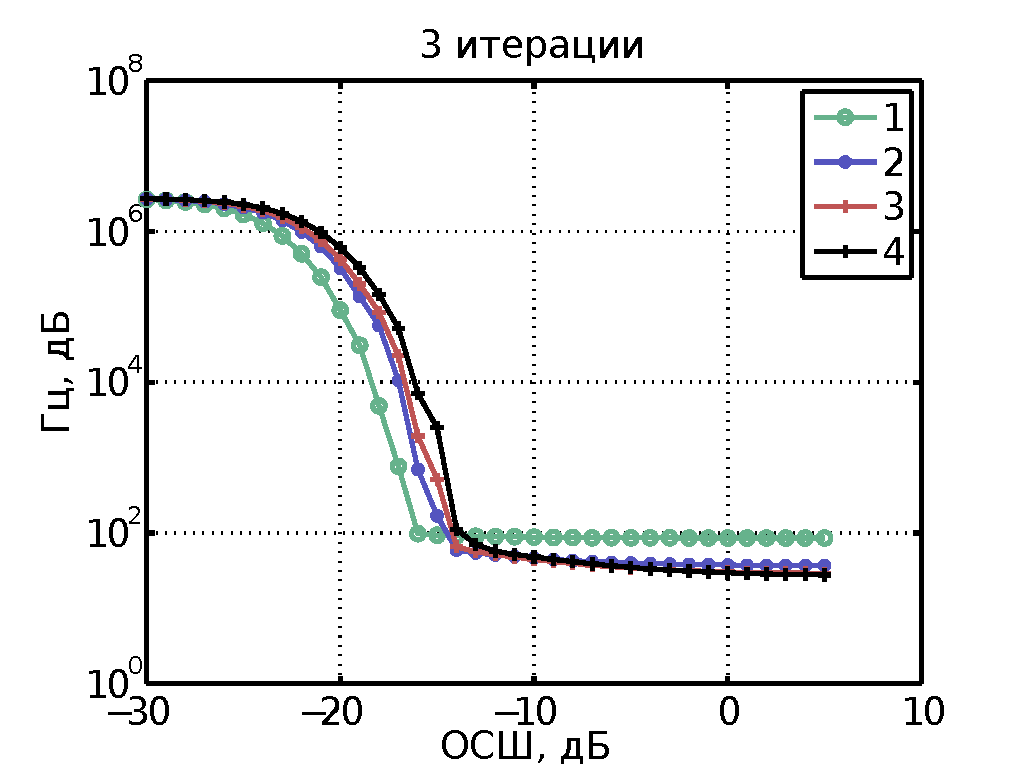
\includegraphics[width=1\linewidth]{fft2_3.eps}}
	\caption{СКО оценки частоты.\\1 - прямоугольное окно, 2 - окно Хемминга, 3 - окно Блекмана, 4 - окно Ханна.}
	\label{pic:fft2_3}
\end{figure}

Из Рис. \ref{pic:fft2_1}, \ref{pic:fft2_2}, \ref{pic:fft2_3} видно, что лучшие результаты показывает подход с применением прямоугольного окна. На Рис. \ref{pic:fft2_rect_1_2_3}
представлен график СКО оценки частоты для одной, двух и трех итераций уточнения АКФ с применением прямоугольного окна. Из \mbox{Рис. \ref{pic:fft2_1}-\ref{pic:fft2_3}}  видно, что большее
количество итераций уточнения позволяет более точно получать оценку на низких ОСШ, вместе с тем точность оценки несколько снижается для ОСШ выше \mbox{-10 дБ.}
\begin{figure}[h]
	\center\scalebox{0.8}{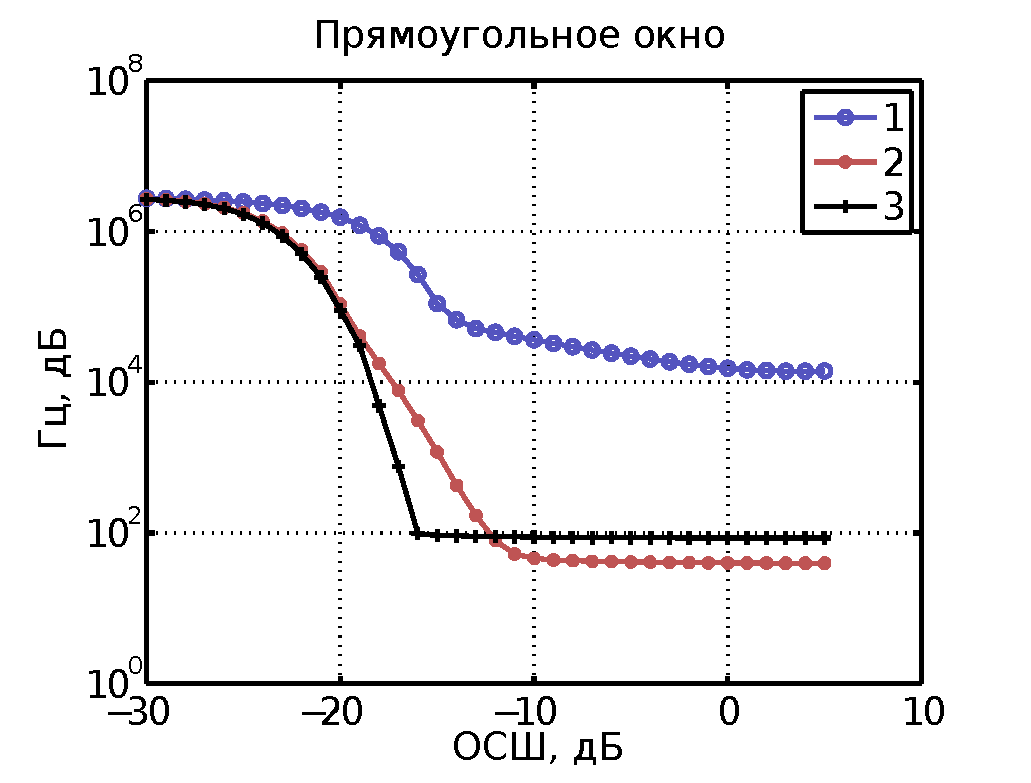
\includegraphics[width=1\linewidth]{fft2_rect_1_2_3.eps}}
	\caption{СКО оценки частоты.\\1 - одна итерация пересчета АКФ, 2 - две итерации пересчета АКФ, 3 - три итерации пересчета АКФ.}
	\label{pic:fft2_rect_1_2_3}
\end{figure}

Представляется интересным изучить влияние длинны блока нулей, дополняющий входную смесь, на СКО оценки частоты. Для решения данной задачи было проведено еще одно моделирование.
На Рис. \ref{pic:fft4_1} представлено моделирование для последовательности дополненной нулями до длинны ${4N}$ с применением различных оконных функций:
прямоугольного окна, окна Хемминга, окна Блекмана и окна Ханна при одной итерации уточнения АКФ.
\begin{figure}[h]
	\center\scalebox{0.8}{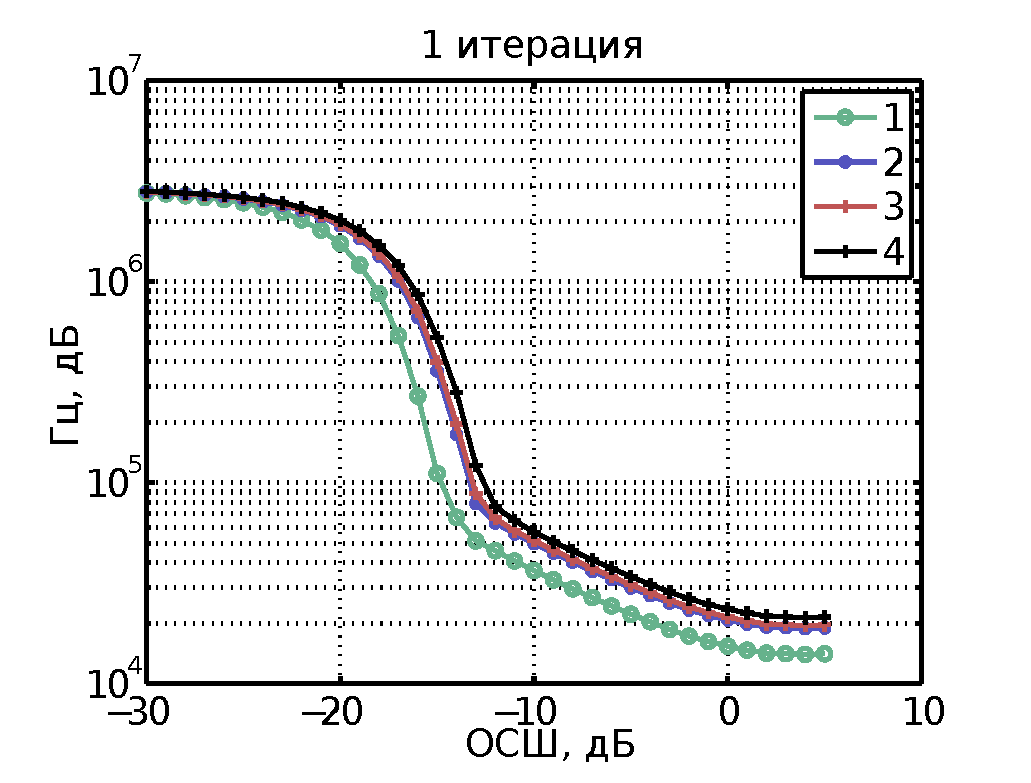
\includegraphics[width=1\linewidth]{fft4_1.eps}}
	\caption{СКО оценки частоты.\\1 - прямоугольное окно, 2 - окно Хемминга, 3 - окно Блекмана, 4 - окно Ханна.}
	\label{pic:fft4_1}
\end{figure}

На Рис. \ref{pic:fft4_2} представлено моделирование для последовательности дополненной нулями до длинны ${4N}$ с применением различных оконных функций:
прямоугольного окна, окна Хемминга, окна Блекмана и окна Ханна при двух итерациях уточнения АКФ.
\begin{figure}[h]
	\center\scalebox{0.8}{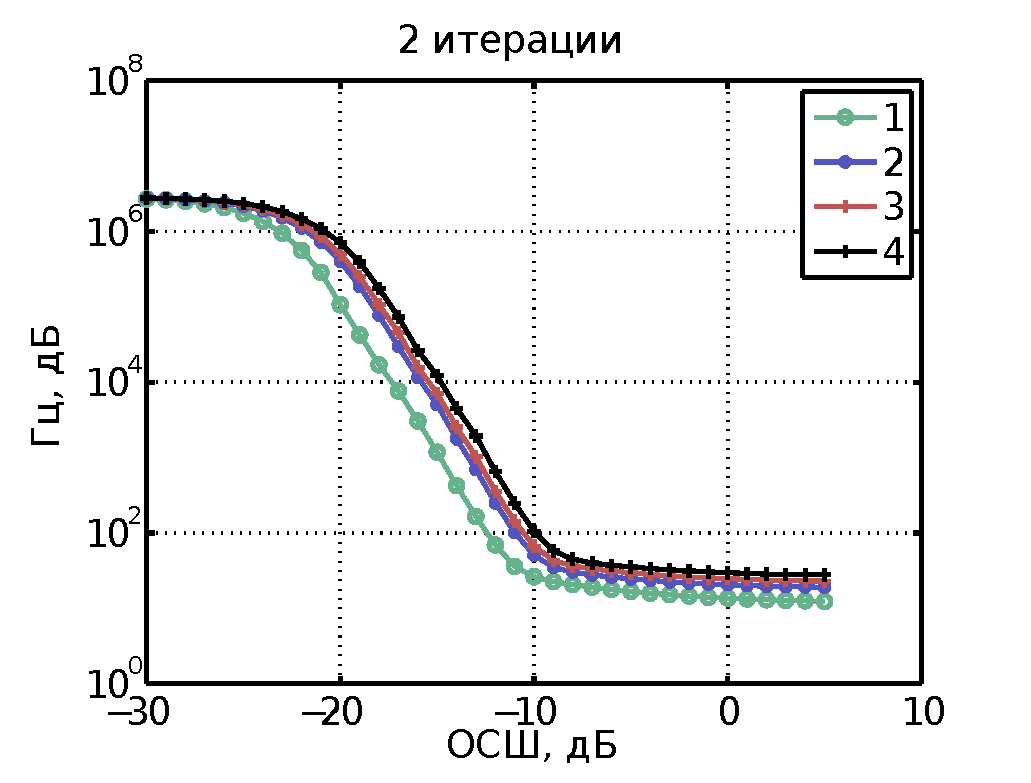
\includegraphics[width=1\linewidth]{fft4_2.eps}}
	\caption{СКО оценки частоты.\\1 - прямоугольное окно, 2 - окно Хемминга, 3 - окно Блекмана, 4 - окно Ханна.}
	\label{pic:fft4_2}
\end{figure}

На Рис. \ref{pic:fft4_3} представлено моделирование для последовательности дополненной нулями до длинны ${4N}$ с применением различных оконных функций:
прямоугольного окна, окна Хемминга, окна Блекмана и окна Ханна при трех итерациях уточнения АКФ.
\begin{figure}[h]
	\center\scalebox{0.8}{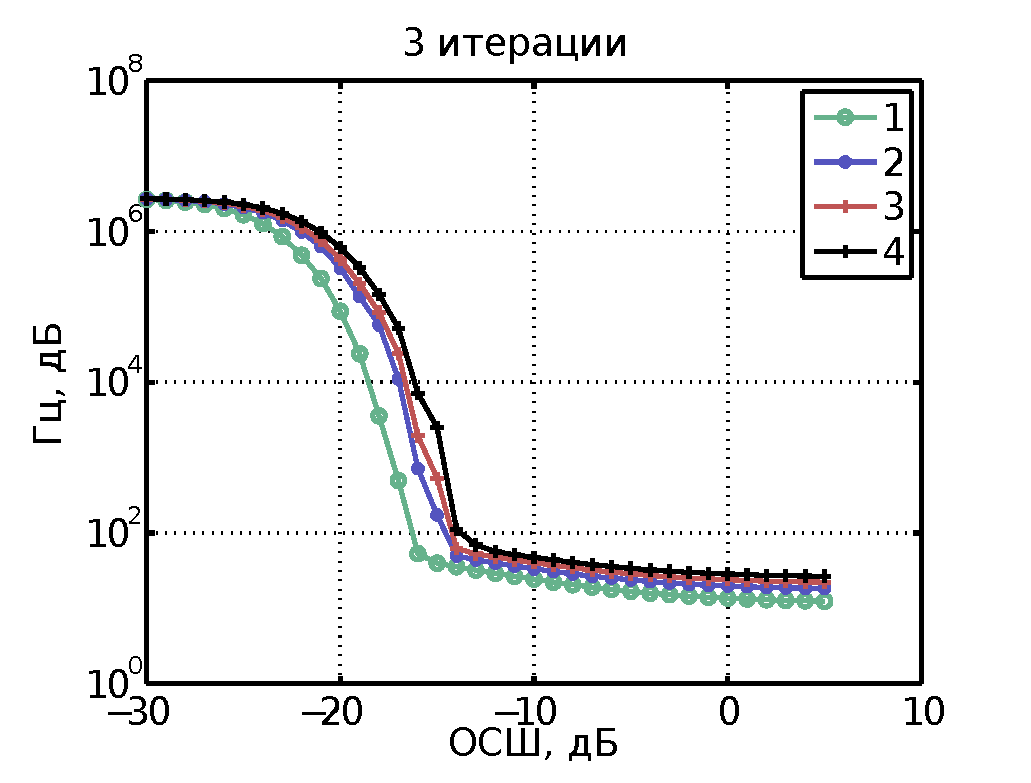
\includegraphics[width=1\linewidth]{fft4_3.eps}}
	\caption{СКО оценки частоты.\\1 - прямоугольное окно, 2 - окно Хемминга, 3 - окно Блекмана, 4 - окно Ханна.}
	\label{pic:fft4_3}
\end{figure}

Из Рис. \ref{pic:fft4_1}, \ref{pic:fft4_2}, \ref{pic:fft4_3} видно, что, также, как и в случае с длинной ${2N}$, лучшие результаты показывает подход с применением прямоугольного окна.
На Рис. \ref{pic:fft4_rect_1_2_3}
представлен график СКО оценки частоты для одной, двух и трех итераций уточнения АКФ с применением прямоугольного окна для блока данных, дополненного нулями до длинны ${4N}$.
Из графиков видно, что большее количество итераций уточнения позволяет более точно получать оценку на низких ОСШ, но в случае с длинной данных ${2N}$ оценки снижалась при
возрастании ОСШ при длине ${4N}$ данного эффекта не наблюдается.
\begin{figure}[h]
	\center\scalebox{0.8}{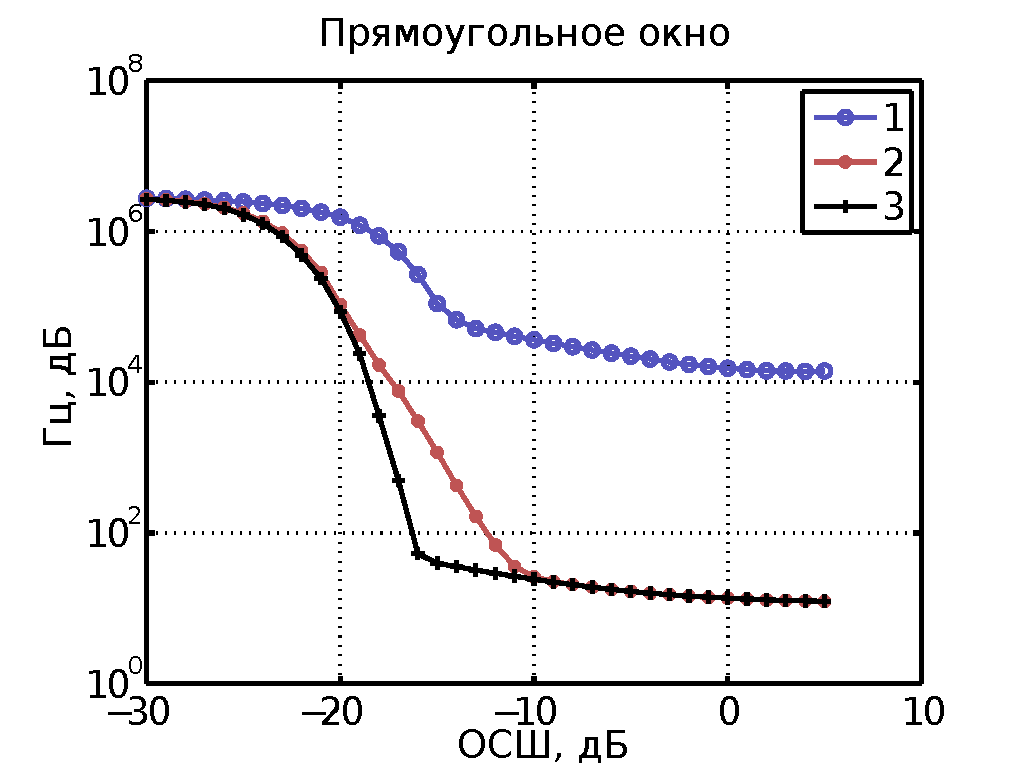
\includegraphics[width=1\linewidth]{fft4_rect_1_2_3.eps}}
	\caption{СКО оценки частоты.\\1 - одна итерация пересчета АКФ, 2 - две итерации пересчета АКФ, 3 - три итерации пересчета АКФ.}
	\label{pic:fft4_rect_1_2_3}
\end{figure}

Из приведенных результатов можно заключить, что наилучшими характеристиками для сигналов с ОСШ ${\le}$ -15 дБ обладает прямоугольное окно. Для сигналов с ОСШ ${\ge}$ 
-15 дБ целесообразно использовать оконное взвешивание. Стоит отметить, что худшими результатами для низких ОСШ (менее 15 дБ) обладает окно Ханна.
Так же из приведенных результатов можно сделать вывод что использование БПФ длиной ${2N}$ нецелесообразно в виду низкой
точности, длины ${4N}$ и ${8N}$ обладают практически одинаковыми характеристиками. Таким образом целесообразно использовать длину ${4N}$. Наилучшие результаты были получены при
использовании трех итераций уточнения АКФ. На Рис. \ref{pic:2vs4vs8} представлена сводка результатов для прямоугольного окна, трех итераций уточнения АКФ и различных длин БПФ.

\begin{figure}[h]
	\center\scalebox{0.8}{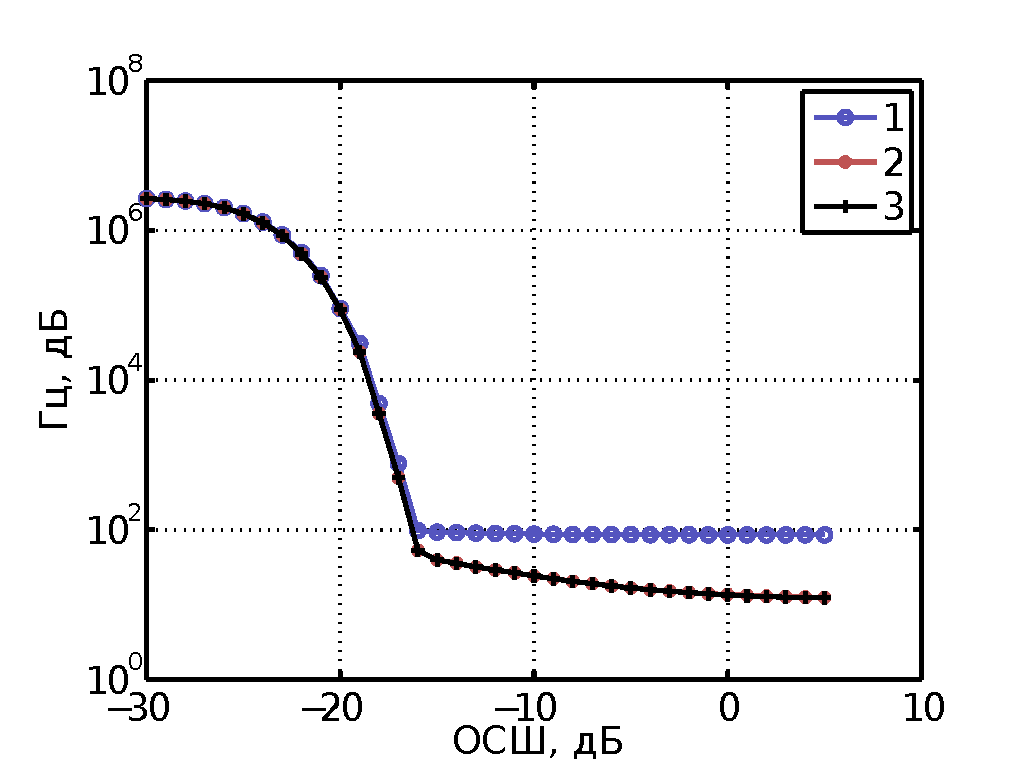
\includegraphics[width=1\linewidth]{2vs4vs8.eps}}
	\caption{СКО оценки частоты.\\1 - БПФ длиной ${2N}$, 2 - БПФ длиной ${4N}$, 3 - БПФ длиной ${8N}$.}
	\label{pic:2vs4vs8}
\end{figure}

%На Рис. \ref{pic:acf_3d} представлен трехмерный график обобщающий опыты проведенные ранее для прямоугольного окна. Из графика видно что длинна БПФ равная ${2N}$ позволяет получить оценку
%с одинаковой точностью для диапазона ${[0, 20]}$ дБ.
%\begin{figure}[h]
%	\center\scalebox{0.8}{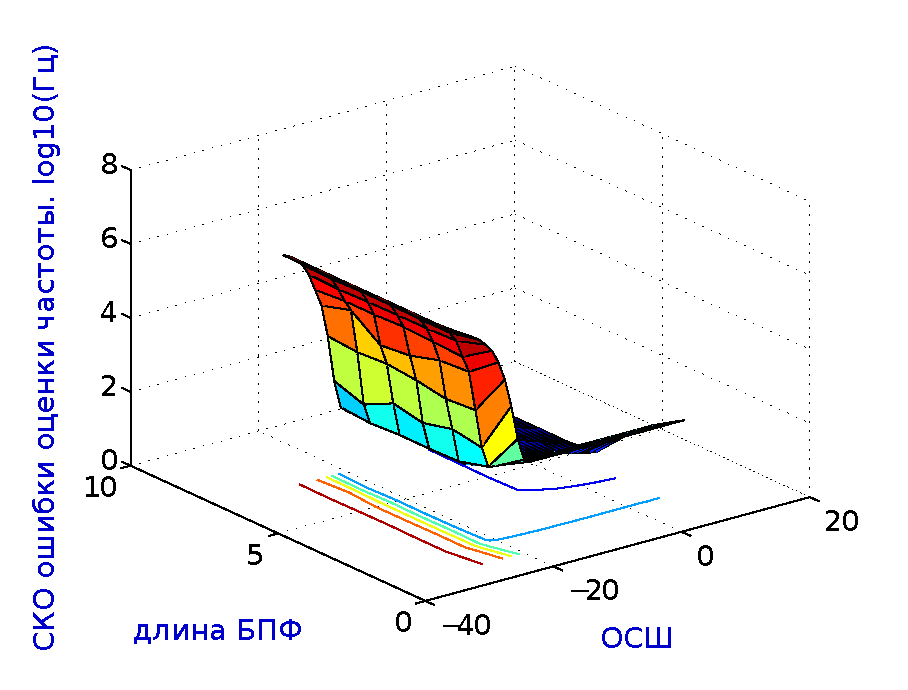
\includegraphics[width=1\linewidth]{acf_3d.eps}}
%	\caption{СКО оценки частоты.}
%	\label{pic:acf_3d}
%\end{figure}

\section{Выводы по Главе 2}

\begin{itemize}
\item АКФ от гармонического сигнала является гармоническим сигналом той же частоты, но с более высоким ОСШ, что позволяет использовать АКФ, полученную итеративно,
	для оценки частоты гармонических компонент, присутствующих во входной смеси.

\item Задача итеративного вычисления оценки АКФ может быть эффективно решена в базисе Фурье.

\item Задача повышения точности оценки частоты в методах с применением АКФ может быть решена при помощи дополнения входной последовательности нулями.

\item В результате имитационного моделирования было получено значение количества нулей и тип функции оконного взвешивания, а также количество итераций уточнения АКФ,
	позволяющих получить оценку частоты, удовлетворяющую входной расстройке ФАПЧ, с использованием АР-модели, при минимальных вычислительных затратах для низких ОСШ.
	Использование прямоугольного окна при дополнении блоком в ${3N}$ нулей (общая длинна последовательности ${4N}$) и трех итерациях уточнения АКФ дает лучше результаты
	для  \mbox{ОСШ ${\le}$ -15 дБ.}

\item Результаты имитационного моделирования показали, что использование окна Ханна для низких ОСШ (менее -15 дБ) дает худшие результаты в сравнении с прямоугольным
	окном и окнами Блекмена и Хемминга.

\end{itemize}

%%%%%%
\clearpage
\addtocontents{toc}{\hfill\par}			% добавить Стр. над номерами страниц
\addtocontents{toc}{~\hfill{Стр.}\par}			% добавить Стр. над номерами страниц
%%%%%%

\clearpage


\section{Глава 3. Алгоритм оценки фазы и частоты ШПС сигнала на основе АР-модели на фоне интерференции}

\subsection{Оценка фазы ПСП в ШПС}
\label{sec_dma_real}
Для использования параметрического метода оценки частоты необходимо восстановить гармоническую форму сигнала. Для этого
нужно получить оценку фазы ПСП и произвести повторную модуляцию входной смеси. Получить оценку фазы ПСП не прибегая к перебору по частоте,
позволяет алгоритм Delay and Multiply Approach (DMA). Данный алгоритм был представлен в статье и книге американского ученого Дж.Цуя \cite{lin_dma, tsui}

Особенностью данного алгоритма является то, что он позволяет свести перебор в двумерной области неопределенности:
промежуточная частота, фаза ПСП к перебору только по фазе ПСП.
Пусть входная смесь представлена выражением \ref{eq:unknown}, а количество источников ${N}$ равно двум. Тогда выражение \ref{eq:unknown} можно переписать в виде:
\begin{center}
\begin{equation}
	\label{eq:dma_cdma_for_2}
	x(m) =	A_1 g_1(t + \tau_1) exp \left[ j \left( \tilde{\omega_1} m + \phi_1 (m) \right) \right]
		+ A_2 g_2(t + \tau_2) exp \left[ j \left(  \tilde{\omega_2} m + \phi_2 (m) \right) \right] + n(m) 
\end{equation}
\end{center}

Следуя алгоритму DMA, необходимо умножить сигнал на задержанную копию:
\begin{center}
\begin{equation}
	\label{eq:dma_cdma_1}
	xx(m) = x(m)x(m+\tau)^*,
\end{equation}
\end{center}
где ${*}$ - операция комплексного сопряжения, ${\tau}$ - задержка между копиями сигнала. Подставляя \ref{eq:dma_cdma_for_2} в \ref{eq:dma_cdma_1} получается выражение:
\begin{center}
\begin{eqnarray}
	\label{eq:dma_cdma_2}
	x(m) & = &[ A_1 g_1(m + \tau_1) exp \left[ j \left( \tilde{\omega_1} m + \phi_1 (m) \right) \right] + \nonumber \\
	     & + & A_2 g_2(m + \tau_2) exp \left[ j \left(  \tilde{\omega_2} m + \phi_2 (m) \right) \right] + n(m) ] + \nonumber \\
	     & + & [A_1 g_1(m + \tau + \tau_1) exp \left[ j \left( \tilde{\omega_1} (m + \tau) + \phi_1 (m + \tau) \right) \right]  + \nonumber \\
	     & + & A_2 g_2(m + \tau + \tau_2) exp \left[ j \left(  \tilde{\omega_2} (m + \tau) + \phi_2 (m + \tau) \right) \right] + n(m + \tau)]^*
\end{eqnarray}
\end{center}

В выражении \ref{eq:dma_cdma_2} полезным слагаемым является:
\begin{center}
\begin{equation}
	\label{eq:dma_cdma_3}
	xx_{sig}(m) = A^2_1 g_{11}(m) exp[j (\tilde {\omega_1} \tau)],
\end{equation}
\end{center}
где ${g_{11}(m)}$ - новая ПСП (структура новых ПСП поясняется ниже). 

Интерференционные помехи, не содержащие полезный сигнал, могут быть представлены как:
\begin{center}
\begin{eqnarray}
	\label{eq:dma_cdma_4}
	xx_{intf}(m) & = & A_{12} g_{12}(m) exp \left[ j \left( \tilde{\omega_1} m - \tilde{\omega_2}(m + \tau) + \phi_{12} (m) \right) \right] + \nonumber \\
		& + & A_{21} g_{12}(m) exp \left[ j \left( \tilde{\omega_2} m - \tilde{\omega_1}(m + \tau) + \phi_{21} (m) \right) \right] + \nonumber \\
		& + & A^2_2 g_{22}(m) exp[j (\tilde {\omega_2} \tau)],
\end{eqnarray}
\end{center}
где ${A_{12}=A_1 A_2}$, ${g_{12}(m)=g(m+\tau+1)g_2(m+\tau_2+\tau)}$, а ${g_{21} = g_2(m+\tau_2)g_1(m+\tau_1+\tau)}$, а ${g_{22}(m)}$ - новая ПСП для источника сигнала 2.

Также появляются новые шумовые компоненты:
\begin{center}
\begin{eqnarray}
	\label{eq:dma_cdma_5}
	xx_{noise}(m) & = & A_{1} g_{1}(m + \tau_1) exp \left[ j \left( \tilde{\omega_1} m + \phi_{1} (m) \right) \right] n(m + \tau) + \nonumber \\
		& + & A_{2} g_{2}(m + \tau_2) exp \left[ j \left( \tilde{\omega_2} m + \phi_{2} (m) \right) \right] n(m + \tau)^* + \nonumber \\
		& = & n(m)A_{1} g_{1}(m + \tau_1 + \tau) exp \left[ j \left( \tilde{\omega_1} (m + \tau) + \phi_{1} (m + \tau) \right) \right] + \nonumber \\
		& + & n(m)A_{2} g_{2}(m + \tau_2 + \tau) exp \left[ j \left( \tilde{\omega_2} (m + \tau) + \phi_{2} (m + \tau) \right) \right] + \nonumber \\
		& + & n(m)n(m+\tau)
\end{eqnarray}
\end{center}

Таким образом \ref{eq:dma_cdma_2} можно переписать как смесь:
\begin{center}
\begin{equation}
	\label{eq:dma_cdma_6}
	xx(m) = xx_{sig}(m) + xx_{intf}(m) + xx_{noise}(m)
\end{equation}
\end{center}

%%%%%%%%%%%%%%%%%%%%%%%%%
\subsection{Алгоритм оценки параметров ШПС в условиях интерференции}
\label{l:ssec3_dma_lpc_algo}

В данной работе предлагается объединить результаты работы алгоритма DMA, рассмотренного в разделе
\ref{sec_dma_real} и, предложенных в данной работе, усовершенствованного итеративного 
алгоритма уточнения АКФ (раздел \ref{sec_acf_fft}) гармонического сигнала и 
подхода для оценки частоты ПСП-модулированного сигнала при помощи АР-модели.

Данный алгоритм был предложен автором на конференции \cite{my_dma_ar}, а так же с некоторыми доработками в \cite{my_otchet}.

Схематично алгоритм изображен на рисунке \ref{pic4:dma_quadruple_lpc}

\begin{figure}[H]
\center\scalebox{1}{\includegraphics[width=1\linewidth]{dma_quadruple_lpc.eps}}
	\caption{Алгоритм обнаружения и оценки параметров ШПС в условиях интерференции (DMA + уточненный АР)}
	\label{pic4:dma_quadruple_lpc}
\end{figure}

Выходом алгоритма DMA является оценка фазы ПСП. Повторно модулируя входящий сигнал ПСП с полученной
фазой, можно восстановить гармонический сигнал. Для оценки частоты данного сигнала применяется
АР-метод. Но для оценки АР-методом, требуется точная оценка АКФ, которую можно получить
с помощью усовершенствованного итеративного алгоритма вычисления АКФ.

Рекомендации по выбору задержки ${\tau}$ и детали алгоритма DMA рассмотрены в разделе
\ref{sec1:dma_real}.

Предложенный алгоритм можно описать следующим набором шагов
\begin{itemize}
\item[Шаг 1.] Входной сигнал ${x(k)}$ умножается на задержанную копию ${x(t-\tau)}$. Так же
	на данном шаге можно производить когерентное накопление результата, для
	увеличения ОСШ.

	\begin{center}
	\begin{equation}
		%\label{}
		x_{new}(k) = \frac{C_{new}(k)}{2} \left(\cos (2\pi f \tau) - \cos \left[2 \pi f (2t - \tau)\right]\right)
	\end{equation}
	\end{center}

\item[Шаг 2.] Полученный сигнал ${x_{new}(k)}$ фильтруется ФВЧ для отсечения высокочастотной компоненты.
\item[Шаг 3.] Генерируется локальная ПСП ${C(k)}$ и умножается на задержанную копию ${C(k-\tau)}$.

	\begin{center}
	\begin{equation}
		%\label{}
		C_{new}(k) = C(k)C(k-\tau)
	\end{equation}
	\end{center}

\item[Шаг 4.] Отфильтрованный сигнал ${x_{filt}(k)}$ коррелируется с новой ПСП ${C_{new}(k)}$
	с использованием БПФ. Выход коррелятора сравнивается с заранее определенным порогом.

	\begin{center}
	\begin{equation}
		%\label{}
		x_{filt}(k) = \frac{C_{new}(k)}{2} \cos (2\pi f \tau)
	\end{equation}
	\end{center}

	\subitem{\bf{Если}}  значение оказалось больше порогового {\bf{то}},
		принимается решение о наличии сигнала. Полученное значение фазы ПСП  - ${m}$ запоминается.
		Перейти на шаг 5.
	\subitem{\bf{Иначе}} 
		Принимается решение об отсутствии сигнала.
\item[Шаг 5.] Входной сигнал ${x(k)}$ модулируется ПСП ${C(k-m)}$. В результате получаем гармонический
	сигнал ${x_{cos}(k)}$ с неизвестной частотой.
\item[Шаг 6.] Для увеличения ОСШ сигнала ${x_{cos}(k)}$ вычисляется значение уточненное значение АКФ
	по алгоритму, предложенному в разделе \ref{l:ssec3_quadruple}.
\item[Шаг 7.] Определяются коэффициенты АР-модели ${\hat{a_1}, \hat{a_2}}$, по формуле \ref{eq:lpc_a_estimation}. 
	Вычисляется резонансная частота ${\omega_0 = 2 \pi f}$ и определяется квадрат модуля частотного отклика АР-модели для этой частоты. 
\end{itemize}

Количество умножений требуемых для оценки частоты одного источника при помощи алгоритма Delay and Multiply Approach и АР-модели:
\begin{enumerate}
\item Алгоритм DMA:
	\begin{center}
	\begin{equation}
		%\label{}
		OP_{DMA} = 8NlogN + 6N
	\end{equation}
	\end{center}
\item Усовершенствованный итеративный алгоритм получения АКФ:
	\begin{center}
	\begin{equation}
		%\label{}
		OP_{ACF} = 8NlogN + (k+2)N
	\end{equation}
	\end{center}
\item Оценка параметра АР-методом:
	\subitem Обращение АКФ матрицы 2x2 элементов требует: 5 умножений, 1 обращение и 1 сложение;
	\subitem Вычисление параметров АР-модели: 4 умножения, 2 сложения;
	\subitem Вычисление полюсов передаточной функции АР-модели: 2 умножения, 3 сложения, 1 операция извлечения корня.

	\begin{center}
	\begin{equation}
		%\label{}
		OP_{AR} = 51
	\end{equation}
	\end{center}
\end{enumerate}

Следует отметить, что в пункте 3 произведены допущения: стоимость 1 операции деления равна 10 операциям умножения, стоимость операции извлечения
корня составляет 20 операций умножения, стоимость сложения не учитывается.
Общее количество умножений для оценки частоты при помощи развиваемого подхода при учете трех итераций уточнения АКФ:
\begin{center}
\begin{equation}
	%\label{}
	OP_{DMA\_ACF\_AR} = 16NlogN + 11N
\end{equation}
\end{center}

%%%%%%%%%%%%%%
\subsection{Сравнительный анализ с параллельным коррелятором}
Структура программного приемника СПИ  Navstar GPS рассмотрена в \cite{tsui}. После стадии оценки параметров сигнала и сравнения с порогом, оценка
частоты для заданного источника поступает в модуль уточнения частоты. Уточненная частота и фаза ПСП поступают в ФАПЧ.
Одним из параметров системы ФАПЧ является шумовая полоса. Этот параметр определяет количество теплового шума попадающего в систему ФАПЧ.
Широкая шумовая полоса позволяет системе ФАПЧ быстро войти в синхронизм, но также ведет к существенному ухудшению характеристик системы ФАПЧ за счет возрастания уровня теплового шума. 

Область синхронизации частоты, в пределах которой не обеспечивается срыв синхронизации, определяется как \cite{spilker-book}:
\begin{center}
\begin{equation}
	\label{eq:pll_omega_m}
	\Delta \omega_m \approx 2 \omega_n (\zeta+0.6),
\end{equation}
\end{center}
где ${\omega_n}$ - собственная частота системы ФАПЧ, ${\zeta}$ - коэффициент демпфирования(${\zeta > 0.3}$).

Примем ${\zeta = 0.707}$. Данное значение   близко к оптимальному \cite{tsui, spilker-book}, тогда ${\Delta \omega_m = 2.614 \omega_n}$.
Собственная частота системы ФАПЧ вычисляется по формуле:
\begin{center}
\begin{equation}
	\label{eq:pll_omega_n}
	\omega_n = \frac{8 \zeta B_L}{4 \zeta^2 + 1},
\end{equation}
\end{center}
где ${B_L}$ - шумовая полоса.

Традиционный подход к оценке параметров широкополосного сигнала предусматривает корреляцию входного сигнала и набора локальных копий сигнала шагом 1 кГц.
Для стационарного приемника СПИ Navstar GPS диапазон смещения частоты, обусловленный Доплеровским эффектом, находится в диапазоне ${\pm 5}$ кГц \cite{tsui, shahtarin_sync}.
Таким образом, для получения оценки с точностью 1 кГц необходимо провести поиск в 11 ячейках. В каждой ячейке нам необходимо ${N}$-комплексных умножений.
Для наземных приемников типовое значение ${B_L=20}$ Гц \cite{tsui}. Область синхронизации из выражений \ref{eq:pll_omega_m} и \ref{eq:pll_omega_n}
${\Delta \omega_m = 100}$ рад/с (примерно 16 Гц). В виду того, что требуемая точность оценки не может быть получена с использованием стандартного шага в 1 кГц,
а использование более мелкого шага ведет к расходованию ресурсов, как уже было отмечено, требуется стадия уточнения частоты.
Схема традиционного приемника изображена на рисунке \ref{pic:corr_scheme}.
\begin{figure}[H]
	\center\scalebox{1}{\includegraphics[width=1\linewidth]{corr_scheme.eps}}
	\caption{Схема традиционного приемника.}
	\label{pic:corr_scheme}
\end{figure}

Количество комплексных умножений требуемых для оценки частоты одного источника при помощи алгоритма БПФ:
\begin{enumerate}
\item ${NlogN}$ - преобразование Фурье входного сигнала;
\item ${N}$ - умножение входного сигнала и локальной копии в Фурье домене;
\item ${N}$ - обратное преобразование Фурье.
\item ${4NlogN}$ - действительных умножений – обратное преобразование Фурье. 
\end{enumerate}

\begin{center}
\begin{equation}
	\label{eq:op_fft}
	OP_{FFT} = NlogN + 11(N + NlogN) = 12NlogN + 11N
\end{equation}
\end{center}

Алгоритм уточнения частоты описан в \cite{tsui}. Данный алгоритм основан на усреднении фазы и требует дополнительной оперативной памяти (ОЗУ) приемника для
хранения 5 миллисекунд данных при обработке одного источника. Оперативная память потребляет значительное количество энергии, поэтому снижение количества
необходимой ОЗУ является важной задачей при разработке портативных приемников. Также обработка 5 мс данных повышает вероятность встретить переход бита
внутри данных – это ведет к дополнительным сложностям при реализации программных приемников сигнала Navstar GPS.

Количество умножений, требуемых для уточнения частоты одного источника:
\begin{enumerate}
\item Повторная модуляция 5 мс данных: ${5N}$ умножений;
\item Повышение точности до 400 Гц: ${6N}$ умножений;
\item Вычисление ДПФ в частотной позиции на длине: ${10N}$ умножений.
\end{enumerate}

\begin{center}
\begin{equation}
	\label{eq:op_fine}
	OP_{FINE} = 21N
\end{equation}
\end{center}

Общее количество операций умножения (количество операций комплексного умножения необходимо домножить на 4):  .
\begin{center}
\begin{equation}
	\label{eq:op_fine_fft}
	OP_{FFT\_FINE} = 48NlogN + 65N
\end{equation}
\end{center}

%%%%%%%%%%%%%%%%
\subsection{Сравнение точности оценки частоты с границей Крамера-Рао}
При разработке алгоритмов оценки параметров полезно иметь некоторую базу для сравнения. Такой базой может быть выбрана граница Крамера-Рао.

Оценка Крамера-Рао тесно связана с понятием эффективности . Данная граница эффективности оценки, улучшить которую невозможно, описывается
неравенством Крамера-Рао-Фреше. Так же известное как неравенство информации.

Если рассматривать класс всевозможных оценок ${\hat{\theta}}$ оцениваемого скалярного параметра ${\theta}$, от которого зависит ПРВ ${f(X; \theta)}$
исследуемой совокупности. Обозначим
\begin{center}
\begin{equation}
	\label{eq:clrb_mean}
	{\bf{E}} \hat{\theta} = \int \hat{\theta} (X_1, ..., X_n)L(X_1, ..., X_n; \theta) dX_1 ... dX_n= \theta + b_{\hat{\theta}}(\theta),
\end{equation}
\end{center}
${b_{\hat{\theta}}(\theta)}$ дает смещение оценки ${\theta}$.

В \cite{ayvazyan-book} приведено, что если  ПРВ ${f(X, \theta)}$  
удовлетворяет некоторым  условиям регулярности (в смысле характера ее зависимости от ${\theta}$), а именно:
\begin{enumerate}
\item область возможных значений исследуемой случайной величины в которой ${f(X; \theta)}$, не зависит от ${\theta}$;
\item в формуле \ref{eq:clrb_mean} и в тождестве ${\int L(X_1, ..., X_n;\theta) dX_1...dX_n = 1}$ допустимо дифференцирование по ${\theta}$ под знаком интеграла;
\item величина ${I(\theta; X)}$ - количество информации Фишера не равна нулю.
\end{enumerate}

Тогда для любой оценки ${\hat{\theta}}$ оцениваемого параметра ${\theta}$ может быть записано неравенство:
\begin{center}
\begin{equation}
	\label{eq:crlb_base3}
	E(\hat{\theta} - \theta) \ge \frac{(1 + \frac{d b_{\hat{\theta}} (\theta)}{d \theta})^2}{n E \left[ \left( \frac{d ln f(X; \theta)}{d \theta} \right)^2 \right]}
\end{equation}
\end{center}

\subsubsection{Граница Крамера-Рао для оценки одной гармонической компоненты}
В данной работе рассматривается оценка частоты одной гармонической компоненты. Поэтому целесообразно рассмотреть только данный случай. В статье \cite{rife-crlb-article}
подробно рассмотрено получение оценки Крамера-Рао для случае одной гармонической компоненты, далее приводится краткая сводка результатов.

Предположим один или несколько параметров сигнала неизвестны. Входная смесь представлена синфазной и квадратурной составляющими. Тогда совместная ПРВ ${\bf{X}}$
при векторе неизвестных параметров ${\bf{\alpha}}$  может быть записана как:
\begin{center}
\begin{equation}
	\label{eq:clrb_pdf}
	f({\bf{X}}; {\bf{\alpha}}) = \left( \frac{1}{\sigma^2 2 \pi} \right)^N exp \left[ -\frac{1}{2\sigma^2} \sum_{n=0}^{N-1} (Re(x)-\mu_n)^2 + (Im(x) - \nu_n)^2 \right],
\end{equation}
\end{center}
где
\begin{center}
\begin{eqnarray}
	\label{eq:clrb_alpha}
	{\bf{\alpha}} & = & [\omega, A, \theta]^T \\
	\mu_n & = & A \cos{(\omega t + \theta)} \\
	\nu_n & = & A \sin{(\omega t + \theta)}
\end{eqnarray}
\end{center}

Несмещенная оценка Крамера-Рао состоит из диагональных элементов матрицы обратной к информационной матрице Фишера ${J}$, таких что
\begin{center}
\begin{equation}
	\label{eq:crlb_Jij}
	J_{ij} = E(H_{\alpha i} H_{\alpha j}) = -E(H_{\alpha i \alpha j}),
\end{equation}
\end{center}
где математическое ожидание с учетом вектора ${\bf{X}}$:
\begin{center}
\begin{equation}
	\label{eq:crlb_H}
	H_{\alpha i} = \frac{\partial}{\partial \alpha_i} \log{f({\bf{X}}; {\bf{\alpha}})}
\end{equation}
\end{center}
Граница задается как:
\begin{center}
\begin{equation}
	\label{eq:crlb_var_alpha}
	D(\hat{\alpha}_i) \ge J^{ii},
\end{equation}
\end{center}
где ${\hat{\alpha}}$ - это оцениваемый параметр ${\alpha_i}$ и ${J^{ii}}$ - ${i}$-й диагональный элемент матрицы ${J^{-1}}$.

Когда ${f({\bf{X}}; {\bf{\alpha}})}$ задана выражением \ref{eq:clrb_pdf}, элементы матрицы ${J}$ могут быть получены с использованием следующего соотношения:
\begin{center}
\begin{equation}
	\label{eq:crlb_Jij_full}
	J_{ij} = \frac{1}{\sigma^2} \sum_{n=0}^{N-1} \left[ \frac{\partial \mu_n}{\partial \alpha_i} \frac{\partial \mu_n}{\partial \alpha_j} + \frac{\partial \nu_n}{\partial \alpha_i} \frac{\partial \nu_n}{\partial \alpha_j} \right]
\end{equation}
\end{center}
Индексы ${i}$ и ${j}$ относятся только к неизвестным параметрам ${\alpha}$.

Наиболее общим случаем для всех параметров ${\alpha}$, матрица ${J}$ из \ref{eq:crlb_Jij_full} принимает вид:
\begin{center}
\begin{equation}
	\label{eq:lpc_a_estimation}
	J = \frac{1}{\sigma^2} =
		\left[ \begin{array}{ccc}
			A_0^2 T^2 (n_0^2 N + 2n_0P + Q) & 0 & A_0^2 T^2 (n_0 N + P) \\
			0 & N & 0 \\
			A_0^2 T^2 (n_0 N + P) & 0 & A_0^2N
		\end{array} \right]
\end{equation}
\end{center}
где
\begin{center}
\begin{eqnarray}
	\label{eq:clrb_QP}
	P & = & \sum_{n=0}^{N-1}n = \frac{N(N-1)}{2} \\
	Q & = & \sum_{n=0}^{N-1}n^2 = \frac{N(N-1)(2N-1)}{6}
\end{eqnarray}
\end{center}

Матрица ${J}$ может быть получена из \ref{eq:crlb_Jij_full} для всех возможных комбинаций. В случае если фаза известна матрица ${J}$ становится матрицей 2x2, после удаления третьей строки
и третьего столбца.

После получения обратной матрицы ${J}$, с учетом всех неизвестных параметров, можно получить следующие выражения.
Для известной фазы и известной или неизвестной амплитуды:
\begin{center}
\begin{equation}
	\label{eq:clrb_est_omega_1}
	D(\hat{\omega}) \ge \frac{\sigma^2}{A_0^2 T^2 (n_0^2 N + 2n_0P + Q)}
\end{equation}
\end{center}

Для неизвестной фазы и известной или неизвестной амплитуды:
\begin{center}
\begin{equation}
	\label{eq:clrb_est_omega_2}
	D(\hat{\omega}) \ge \frac{12\sigma^2}{A_0^2 T^2N(N^2-1)}
\end{equation}
\end{center}

Для всех случаев:
\begin{center}
\begin{equation}
	\label{eq:clrb_est_b_1}
	D(\hat{A}) \ge \frac{\sigma^2}{N}
\end{equation}
\end{center}

Для известной частоты и известной или неизвестной амплитуды:
\begin{center}
\begin{equation}
	\label{eq:clrb_est_b_1}
	D(\hat{\theta}) \ge \frac{\sigma^2}{A_0^2N}
\end{equation}
\end{center}

Для неизвестной частоты и известной или неизвестной амплитуды:
\begin{center}
\begin{equation}
	\label{eq:clrb_est_b_1}
	D(\hat{\theta}) \ge \frac{12\sigma^2(n_0N + 2n_0P + Q)}{A_0^2N(N^2-1)}
\end{equation}
\end{center}

\subsubsection{Сравнение предлагаемого алгоритма с границей Крамера-Рао}
\begin{figure}[H]
\center\scalebox{1}{\includegraphics[width=1\linewidth]{crlb_vs_algorithm.eps}}
	\caption{СКО оценки частоты при использовании итеративного алгоритма оценки АКФ и АР модели}
	\label{pic:crlb_vs_algorithm}
\end{figure}

Из рисунка \ref{pic:crlb_vs_algorithm} видно, что используя итеративный алгоритм вычисления АКФ можно получить заданную точность
при ОСШ -13 дБ для 2 итераций и -20 дБ для 3 итераций. Моделирование проводилось на частоте кратной частоте дискретизации для
того чтобы избежать эффектов растекания спектра. Данные эффекты можно частично компенсировать дополнением нулями в
усовершенствованном итеративном алгоритме получения АКФ. Это было учтено при полунатурном моделировании.

\subsection{Выводы}
%В данном случае необходима стадия уточнения частоты. Следует отметить, что заданная точность может быть достигнута даже на сигнале с достаточно
%низким ОСШ при оценке АР-методом после уточнения АКФ – рисунок 8.

В данной главе рассмотрен метод оценки параметров ШПС. Проведено сравнение с существующим методом оценки параметров СПИ с ШПС. На основании рассмотренного материала можно заключить:
\begin{enumerate}
\item Особенностью СПИ с ШПС является наличие ярко выраженного одиночного пика на ПЧ в спектральной области сигнала после повторной модуляции с ПСП.
	Этот факт дает основания полагать, что такие сигналы могут быть достаточно точно представлены с помощью АР(2).
\item Использование процедуры оценки параметров АР(2) вместо перебора по заранее заданным значениям позволяет вести поиск сигнала в широком диапазоне частот и определять сдвиг
	с более высокой точностью, устраняя необходимость дополнительного уточнения доплеровского сдвига перед запуском процедуры сопровождения сигнала.
\item Точность оценок, полученных на основе АР(2) быстро снижается при наличии сильного или окрашенного шума. Для преодоления указанных трудностей в 
	данной работе предлагается использовать усовершенствованный итеративный алгоритм уточнения АКФ (глава \ref{sec_acf_fft}).
\item Вычислительные затраты предложенного алгоритма составляют   операций умножения, что значительно ниже чем   для традиционного алгоритма параллельного коррелятора.
\end{enumerate}

Сказанное выше позволяет заключить, что разработанный алгоритм может применяться в задачах оценки параметров СПИ с ШПС в случаях когда размер выборки ограничен и
требуется повышенная точность оценки доплеровского сдвига частоты. К недостаткам метода следует отнести высокие требования к точности выполнения математических операций.
Так, например, при вычислении полюсов передаточной функции АР модели необходимо использовать вычисления в формате с плавающей точкой. 
Как уже было сказано, моделирование проводилось на частоте, кратной частоте дискретизации. Данное ограничение можно преодолеть используя дополнение нулями при оценке АКФ
в усовершенствованном алгоритме оценки АКФ.

\newpage


\chapter{Полунатурное моделирование}
\label{ss:hw}

Задачей полунатурного эксперимента являлась верификации возможности применения предлагаемого подхода к оценке параметров сигнала СПИ с ШПС. Для определения наличия источников
сигнала был применен классический параллельный коррелятор \cite{tsui} с шагом по частоте 1 кГц и диапазоном 5 кГц. Данный диапазон обусловлен максимальным Допплеровским
смещением частоты для стационарного приемника в СПИ Navstar GPS \cite{shahtarin_sync, tsui}. 

\section{Аппаратная платформа}
Представленная аппаратная платформа была разработана автором в процессе дипломного проектирования в Московском Государственном Университете Приборостроения и Информатики (МГУПИ).

Данная аппаратная платформа предоставляет пользователю возможность получать необработанный сигнал со спутников СНС Navstar GNSS. В текущей реализации поддерживается только 
СНС Navstar GPS, однако чип так же может принимать сигналы СНС Galileo и СНС Глонасс. Дампы данных представляют собой текстовые файлы. В них содержится 256 КБ необработанных данных.
На частоте оцифровки 256 КБ представляет чуть более 6 мс данных. Данного объема хватает для оценки параметров источников сигналов СНС Navstar GPS.
В данный момент аппаратная платформа используется как лабораторный стенд в МГУПИ по курсу ЦОС. Платформа позволяет работать с реальным сигналом, что является большим плюсом в
виду того, что позволяет наглядно продемонстрировать работу алгоритмов обработки сигнала, а так же проверить теоретические предположения в реальных условиях.
Так же на базе платы разрабатывается ряд дипломных работ в области СНС систем (например создание аппаратного коррелятора на VHDL или создание модели канала 
СПИ Navstar GPS данных). Исходники прошивки платы расположены в публично доступном хранилище кода github.com \cite{github-gpsproject}.
Там же опубликована разводка платы в формате программы PCAD и BOM (bill of materials).

Компонентами на плате управляет FPGA-микросхема. В ней содержится контроллер памяти, реализация RS-232 интерфейса, последовательный интерфейс программирования микросхемы
MAX2769 компании Maxim Semiconducter, модуль захвата данных, а так же вспомогательные модули. В рабочем режиме плата ждет команд с RS-232 интерфейса.
Команды выдает управляющее ПО (board daemon) - сервис разработанный под ОС GNU Linux.

Схема аппаратного обеспечения, настроенного на двухквадратурный прием сигнала СНС Navstar GPS с двухбитным режимом работы АЦП, приведена на Рис. \ref{pic:board_scheme}.
\begin{figure}[h]
	\center\scalebox{1}{\includegraphics[width=1\linewidth]{board_scheme.eps}}
	\caption{Схема аппаратного обеспечения}
	\label{pic:board_scheme}
\end{figure}

Схема системы по захвату данных представлена на Рис. \ref{pic:gps_acq_system_scheme}. Данная система работает по схеме отложенной обработки данных. Основной сервер системы захвата
выдает команду оборудованию захвата - начать накопление данных. Оборудование захвата данных переходит в режим захвата и начинает накапливание 256 КБ данных. По окончании цикла
накопления данных оборудование захвата данных отвечает о готовности данных основному серверу системы захвата и начинает передачу данных. После передачи данных основной сервер
захвата данных публикует на публичный FTP-сервер файл с данными и прилагает к нему WAAS-картинку, которая отображает положения спутников над землей. Файл с данными
и картинку WAAS может забрать с FTP-сервера клиент для последующей работы с данными на своем ПК. В качестве диплома автор также разработал SDK для работы с файлом данных
\cite{github-gpsproject}: функции загрузки данных в MATLAB, параллельный коррелятор, генератор ПСП Голда и некоторые другие функции для облегчения работы с аппаратной платформой
и данными.

\begin{figure}[h]
	\center\scalebox{1}{\includegraphics[width=1\linewidth]{gps_acq_system_scheme.eps}}
	\caption{Схема системы захвата данных}
	\label{pic:gps_acq_system_scheme}
\end{figure}

Структура файла с данными представлена на Рис. \ref{pic:dump_file}. В файл записываются значения управляющих регистров микросхемы MAX2769 для того, чтобы можно было
понять в каком режиме был записан файл. К доступным режимам, например, можно отнести \cite{max2769_manual}: одно- или двухквадратурный режим работы, разрядность при оцифровке
аналогового сигнала, тип захватываемых данных СНС (Глонасс, Navstar GPS, Galileo), а так же другие.
\begin{figure}[h]
	\center\scalebox{0.5}{\includegraphics[width=1\linewidth]{dump_file.eps}}
	\caption{Структура файла с данными}
	\label{pic:dump_file}
\end{figure}

Полученный файл с данными оцифрован с частотой 16.368 МГц, ПЧ источников сигнала, 4.092 МГц. В качестве алгоритма оценки фазы ПСП использовался рассмотренный алгоритм DMA,
оценка частоты проводилась при помощи алгоритма основанного на применении авторегрессионной модели (АР), предложенной авторами в \cite{my_otchet}. Полученная оценка
частоты классическим коррелятором и предлагаемым алгоритмом сравнивалась (с точностью до 1 кГц), при это оценка фазы ПСП должна находиться в пределах одного чипа: ${\pm 8}$
отсчетов. При совпадении оценки фазы ПСП и оценки частоты, оценка частоты полученная предлагаемым алгоритмом подавалась на классический коррелятор для повторной проверки.

Для увеличения ОСШ в алгоритме DMA использовалось когерентное накопление сигнала. Производилось осреднение на 3 мс сигнала, что дает прирост ОСШ на 4.77 дБ.
В алгоритме на основе АР метода была взята 1 мс сигнала дополненная 3 мс нулей, для повышения спектрального разрешения при оценке АКФ посредством ДПФ.

\subsection{Результаты эксперимента}

Результат работы классического коррелятора представлены на Рис. \ref{pic:16mhz_sats_all}. Сигнал взят с 2000 отсчета, данное смещение выбрано произвольно.
\begin{figure}[h]
\center\scalebox{1}{\includegraphics[width=1\linewidth]{16mhz_sats_all.eps}}
	\caption{Соотношений энергий источников сигнала}
	\label{pic:16mhz_sats_all}
\end{figure}

В виду того, что данных недостаточно для запуска модуля ФАПЧ, целесообразно рассматривать фазу ПСП и оценку частоты для сравнения работы двух
алгоритмов - таблица \ref{tbl:16mhz_sats_all} отражает данные с Рис. \ref{pic:16mhz_sats_all}.
\begin{center}
	\begin{longtable}{ | c | c | c | c |}
	\hline
	Источник сигнала & Фаза ПСП & Оценка частоты, Гц & Величина пика КФ, дБ \\ \hline
	01 & 14213	& 4091000.00	& 10.93 \\ \hline 
	02 & 4788	& 4087000.00	& 10.47 \\ \hline
	03 & 4750	& 4092000.00	& 10.59 \\ \hline
	04 & 8319	& 4097000.00	& 10.43 \\ \hline
	05 & 14143	& 4091000.00	& 10.75 \\ \hline
	06 & 7270	& 4089000.00	& 11.47 \\ \hline
	07 & 7829	& 4088000.00	& 10.46 \\ \hline
	08 & 1988	& 4092000.00	& 10.45 \\ \hline
	09 & 3571	& 4094000.00	& 10.53 \\ \hline
	10 & 2872	& 4093000.00	& 10.35 \\ \hline
	11 & 1353	& 4089000.00	& 11.09 \\ \hline
	12 & 13042	& 4097000.00	& 10.39 \\ \hline
	13 & 16311	& 4096000.00	& 10.49 \\ \hline
	14 & 11158	& 4092000.00	& 10.79 \\ \hline
	15 & 5297	& 4089000.00	& 10.86 \\ \hline
	16 & 14905	& 4094000.00	& 11.41 \\ \hline
	17 & 10017	& 4093000.00	& 11.29 \\ \hline
	18 & 11500	& 4087000.00	& 10.61 \\ \hline
	19 & 14434	& 4088000.00	& 12.57 \\ \hline
	20 & 14026	& 4094000.00	& 10.33 \\ \hline
	21 & 13463	& 4087000.00	& 10.25 \\ \hline
	22 & 2251	& 4094000.00	& 11.64 \\ \hline
	23 & 15352	& 4091000.00	& 10.55 \\ \hline
	24 & 14627	& 4094000.00	& 11.55 \\ \hline
	25 & 9910	& 4093000.00	& 11.10 \\ \hline
	26 & 934	& 4087000.00	& 10.73 \\ \hline
	27 & 8090	& 4091000.00	& 11.28 \\ \hline
	28 & 13998	& 4090000.00	& 11.29 \\ \hline
	29 & 6503	& 4087000.00	& 10.99 \\ \hline
	30 & 13592	& 4094000.00	& 12.87 \\ \hline
	31 & 4505	& 4092000.00	& 15.57 \\ \hline
	32 & 10210	& 4092000.00	& 15.50 \\ \hline
	\caption{Соотношений энергий источников сигнала}
	\label{tbl:16mhz_sats_all}
	\end{longtable}
\end{center}

Рассмотрим источники сигнала с номерами 31 и 32 как наиболее сильные.

Рассмотрим источник сигнала 31. Сравнение полученных оценок представлено в таблице \ref{tbl:16mhz_sat_31}. Оценки, полученные с использованием
предлагаемого подхода согласуются с результатами, полученными классическим подходом.
\begin{center}
	\begin{longtable}{ | c | c | c | c |}
	\hline
	Алгоритм	& Оценка фазы ПСП & Оценка частоты, Гц & Величина пика КФ, дБ \\ \hline
	АР + DMA	& 4503 & 4092277.39	& 15.60 \\ \hline
	Коррелятор & 4505 & 4092000.00	& 15.57 \\ \hline
	\caption{Оценка параметров источника сигнала 31}
	\label{tbl:16mhz_sat_31}
	\end{longtable}
\end{center}

Так же рассмотрим источник сигнала 32.  Сравнение полученных оценок представлено в таблице \ref{tbl:16mhz_sat_32}. Оценки, полученные с использованием
предлагаемого подхода согласуются с результатами, полученными классическим подходом.
\begin{center}
	\begin{longtable}{ | c | c | c | c |}
	\hline
	Алгоритм	& Оценка фазы ПСП & Оценка частоты, Гц & Величина пика КФ, дБ \\ \hline
	АР + DMA	& 10210 & 4091937.35	& 15.56 \\ \hline
	Коррелятор	& 10209 & 4092000.00   	& 15.50 \\ \hline
	\caption{Оценка параметров источника сигнала 32}
	\label{tbl:16mhz_sat_32}
	\end{longtable}
\end{center}

Из таблиц \ref{tbl:16mhz_sat_31} и \ref{tbl:16mhz_sat_32} видно, что применение предлагаемого подхода позволяет получить более точные оценки частоты. Данные
результаты согласуются с известными результатами.

%%%%%%
%\clearpage
\section{Эксперимент на данных Мишеля Боваро}

Так же полунатурное моделирование проводилось с данными собранными итальянским ученым Мишелем Боваро (Michele Bavaro) \cite{bovaro_blog}. Представленный файл с данными оцифрован
с частотой 5.456 МГц, промежуточная частота источников сигнала, 4.092 МГц. Длинна записанных данных позволяет так же проверить
вхождение системы в синхронизм. Файл больше недоступен по ссылке, приведенной в блоге Мишеля Боваро, автор представляет его по адресу \cite{rflab_primo}.
Объема данных достаточно для оценки информационных параметров и проверки вхождения с синхронизм. По этой причине в данной диссертационной работе будет
рассмотрена система ФАП, оптимальная для приема 2-ФМ манипулированного сигнала.

В качестве алгоритма оценки фазы ПСП использовался
рассмотренный алгоритм DMA, оценка частоты проводилась при помощи алгоритма основанного на применении авторегрессионной модели (АР).
Полученная оценка подавалась на модуль фазовой автоподстройки частоты (ФАПЧ) и проверялось вхождение в синхронизм.

Для увеличения ОСШ в алгоритме DMA использовалось когерентное накопление сигнала. Производилось осреднение на 3 мс сигнала, что дает прирост ОСШ на 4.77 дБ.
В алгоритме на основе АР метода была взята 1 мс сигнала дополненная 3 мс нулей, для повышения спектрального разрешения при оценке АКФ посредством ДПФ.

В качестве модуля ФАПЧ взят код американского ученого Дениса Акоса (Dennis M. Akos) \cite{sandiaproject}.
Параметры выбранные для ФАПЧ: коэффициент демпфирования ${\zeta=0.7}$, шумовая полоса  ${B_L=40}$ Гц. 

%%%
\subsection{Схема Костаса}

При использовании схемы Костаса осуществляется демодуляция 2-ФМ сигналов, при этом используется фазовая автоматическая подстройка (ФАП) частоты. Схема
Костаса является оптимальной \cite{shahtarin-wiener-kalman}.

В основе оптимальной нелинейной фильтрации лежит уравнение Р.Л. Стратоновича. Так как уравнение Стратоновича в общем виде решению не поддается, необходимо
перейти к системе двух уравнений:
\begin{itemize}
	\item дифференциальное уравнение относительно оцениваемых параметров;
	\item дифференциальное уравнение относительно дисперсии ошибки.
\end{itemize}

Так как приведенные уравнения являются нелинейными, при их составлении необходимо задать функцию Стратановича.

Входная смесь, содержащая 2-ФМ сигнал, может быть представлена в виде:
\begin{equation}
	x(t) = s(t, \varphi, \alpha) + n(t) = A \cos \left[ \omega_0t + \varphi(t) +\alpha \pi \right] + n(t),
	\label{eq:sec4_sig}
\end{equation}
где ${n(t)}$ - АБГШ, ${\alpha}$ принимает дискретные значения 1 или 0, амплитуда ${A}$ и частота ${\omega}$ постоянны.

Уравнения фильтрации имеют вид:
\begin{eqnarray}
	\frac{d \hat{\varphi}}{dt} = \sigma_{\hat{\varphi}}^2(p_1 F_{1}' + p_2 F_{2}'), \nonumber \\
	\frac{d \sigma_{\hat{\varphi}}^2}{dt} = \frac{1}{2}N_{\varphi} + \sigma_{\hat{\varphi}}^4(p_1 F_{1}'' + p_2 F_{2}''),
	\label{eq:sec4_filter_eq}
\end{eqnarray}
где ${p_1, p_2}$ - апостериорные вероятности состояния параметра ${\alpha}$, ${\hat{\varphi}}$ - оценка параметра ${\varphi}$, а ${\sigma_{\hat{\varphi}}^2}$ - 
дисперсия параметра ${\hat{\varphi}}$, ${N_{\varphi}}$ - односторонний энергетический спектр, ${F_i(t, \varphi)}$ - функция Стратоновича.
\begin{equation}
	F_i(t, \varphi) = \frac{2}{N_0} x(t)s(t, \varphi, \alpha_i),
	\label{eq:sec4_stratonovicha_eq}
\end{equation}
где ${i = 1, 2}$, а ${\alpha_1 = 0}$ и ${\alpha_2 = 1}$.

\begin{eqnarray}
	F_{i}' = \frac{\partial{F_i (t, \hat{\varphi})}}{\partial{\hat{\varphi}}}, \nonumber \\
	F_{i}'' = \frac{\partial^2{F_i (t, \hat{\varphi})}}{\partial{\hat{\varphi}^2}}.
	\label{eq:sec4_stratonovicha_eq_der}
\end{eqnarray}

Дифференциальные уравнение, записанные относительно  апостериорных вероятностей ${p_i}$ \cite{shahtarin-wiener-kalman}:
\begin{eqnarray}
	\frac{dp_1}{dt} = -\mu p_1 + \nu p_2 + p_1 p_2 \left[ (F_1 - F_2) + \frac{1}{2} p_1 \sigma_{\hat{\varphi}}^2 (F_1'' - F_2'') \right]; \nonumber \\
	\frac{dp_2}{dt} = \mu p_1 - \nu p_2 - p_1 p_2 \left[ (F_1 - F_2) + \frac{1}{2} p_2 \sigma_{\hat{\varphi}}^2 (F_1'' - F_2'') \right],
	\label{eq:sec4_stratonovicha_eq_der_p}
\end{eqnarray}
где ${\mu, \nu}$ - элементы матрицы интенсивностей вероятностей перехода дискретного процесса ${\alpha(t)}$:
\begin{equation}
	\label{eq:sec4_alpha}
	\{\alpha_{ij}\}
	=
		\left[ \begin{array}{cc}
			-\mu	&	\mu \\
			\nu 	&	-\nu
		\end{array} \right],
\end{equation}
где ${i,j = 1,2}$.

Принятие решения о значении параметра ${\alpha}$ возможно по значению знака разности апостериорных вероятностей ${z = p_1 - p_2}$. В данном случае
при учете соотношений:
\begin{eqnarray}
	p_1 + p_2 = 1; \nonumber \\
	p_1 = \frac{1+z}{2}; \nonumber \\
	p_2 = \frac{1-z}{2}.
	\label{eq:sec4_probability}
\end{eqnarray}

Количество уравнений системы может быть сокращено до трех:
\begin{eqnarray}
	\frac{d \hat{\varphi}}{dt} & = & \frac{1}{2}\sigma_{\hat{\varphi}}^2 \left[(F_{1}' + F_{2}') + z(F_{1}' - F_{2}') \right]; \nonumber \\
	\frac{d \sigma_{\hat{\varphi}}^2}{dt} & = & \frac{1}{2}N_{\varphi} + \frac{1}{2}\sigma_{\hat{\varphi}}^4 \left[ (F_{1}'' + F_{2}'') +  z(F_{1}'' - F_{2}'') \right]; \\
	\frac{dz}{dt} & = & (\nu - \mu) - (\nu + \mu)z + \frac{1}{2}(1 - z^2) \left[ (F_{1} - F_{2}) +  \frac{1}{2} \sigma_{\hat{\varphi}}^2 (F_{1}'' - F_{2}'') \right]. \nonumber
	\label{eq:sec4_stratonovich_3}
\end{eqnarray}

В случае когда принимаемый сигнал модулирован оп закону 2-ФМ, когда параметра ${\alpha}$ принимает два дискретных значения 0 и 1,
функция Стратоновича записывается как \cite{shahtarin-wiener-kalman}:
\begin{equation}
	F_1(t, \varphi) = \frac{2A}{N_0}x(t) \cos (\omega_0 t + \varphi) = -F_2(t, \varphi)
	\label{eq:sec4_stratonovich_bpsk}
\end{equation}

Сигналы ${s_1(t)}$ и ${s_2(t)}$ определяются равенством: 
\begin{equation}
	s_1(t, \varphi) = -s_2(t, \varphi) = A \cos \left[ \omega_0 t \varphi(t) \right].
	\label{eq:sec4_s1_s2}
\end{equation}

В данном случае:
\begin{eqnarray}
	F_1' + F_2' & = & 0; \nonumber \\
	F_1'' + F_2'' & = & 0; \nonumber \\
	F_1 - F_2 & = & 2F_1 = \frac{4A}{N_0}x(t) \cos(\omega_0 t + \hat{\varphi}); \nonumber \\
	F_1' - F_2' & = & 2F_1' = -\frac{4A}{N_0}x(t) \sin(\omega_0 t + \hat{\varphi}); \nonumber \\
	F_1'' - F_2'' & = & 2F_1'' = -\frac{4A}{N_0}x(t) \cos(\omega_0 t + \hat{\varphi}) = -2F_1. \nonumber \\
	\label{eq:sec4_strat_der}
\end{eqnarray}

При ${\nu = \mu = \frac{1}{2}}$ выражения \ref{eq:sec4_stratonovich_3} принимают вид:
\begin{eqnarray}
	\frac{d \hat{\varphi}}{dt} + \frac{2A}{N_0} \sigma_{\hat{\varphi}}^2 z x(t) \sin (\omega_0 t + \hat{\varphi}) & = & 0; \nonumber \\
	\frac{d \hat{\varphi}^2}{dt} = \frac{1}{2} N_{\varphi} - \sigma_{\hat{\varphi}}^4 z \frac{2A}{N_0} x(t) \cos(\omega_0 t + \hat{\varphi}) & = & \frac{1}{2}N_{\varphi} - \sigma_{\hat{\varphi}}^4 zF_1(t, \hat{\varphi}); \nonumber \\
	\frac{dz}{dt} = -z + (1 - z^2) \left( 1 - \frac{1}{2} \sigma_{\hat{\varphi}}^2 \right) x(t) \cos(\omega_0 t + \hat{\varphi}) & = & \nonumber \\
		 = -z + (1 - z^2) \left( 1 - \frac{1}{2} \sigma_{\hat{\varphi}}^2 \right) F_1(t, \hat{\varphi}), & &
	\label{eq:sec4_strat_der111}
\end{eqnarray}
в тоже время ${1 - z^2 \ge 0}$.


В случае ${z=th \int_{t_k}^t F_1(t, \hat{\varphi}) \hat{d\varphi}}$ схема алгоритма соответствует оптимальному приемнику, по критерию МАВ \cite{shahtarin-wiener-kalman}, а при ${thx \approx x}$
соответствует схеме Костаса.

\begin{figure}[h]
\center\scalebox{1}{\includegraphics[width=1\linewidth]{costas.eps}}
	\caption{Схема Костаса}
	\label{pic:sec4_costas}
\end{figure}

На Рис. \ref{pic:sec4_costas} представлена схема Костаса, где СД - синхронный детектор, ФНЧ - фильтр нижних частот, УГ - управляемый генератор, ${\Phi_z}$ - формирователь величины ${z}$,
${\hat{\alpha}}$ - оценка параметра ${\alpha}$, ${\alpha}$, а ${\sigma_{\hat{\varphi}}^2}$ значение дисперсии ${\hat{\varphi}}$, ${a_1 = \frac{2A}{N_0} \sigma_{\hat{\varphi}}^2}$.

\subsection{Результаты эксперимента}

Результат работы классического коррелятора представлены на Рис. \ref{pic:5mhz_sats_all}. Сигнал взят с 2000 отсчета, данное смещение выбрано произвольно.
\begin{figure}[h]
\center\scalebox{1}{\includegraphics[width=1\linewidth]{5mhz_sats_all.eps}}
	\caption{Соотношений энергий источников сигнала}
	\label{pic:5mhz_sats_all}
\end{figure}

В таблице \ref{tbl:5mhz_sats_all} представлены оценки фаз ПСП и частот для Рис. \ref{pic:5mhz_sats_all}.
\begin{center}
	\begin{longtable}{ | c | c | c | c |}
	\hline
	Источник сигнала & Фаза ПСП & Оценка частоты, Гц & Величина пика КФ, дБ \\ \hline
	01 & 3056 & 4093000.00 & 14.64 \\ \hline 
	02 & 776  & 4090000.00 & 9.79  \\ \hline
	03 & 2372 & 4087000.00 & 10.33 \\ \hline
	04 & 1951 & 4089000.00 & 10.79 \\ \hline
	05 & 1231 & 4093000.00 & 12.11 \\ \hline
	06 & 3565 & 4087000.00 & 10.72 \\ \hline
	07 & 4576 & 4091000.00 & 9.79  \\ \hline
	08 & 1177 & 4097000.00 & 10.25 \\ \hline
	09 & 4665 & 4090000.00 & 10.08 \\ \hline
	10 & 387  & 4088000.00 & 10.03 \\ \hline
	11 & 3805 & 4095000.00 & 10.74 \\ \hline
	12 & 762  & 4094000.00 & 11.00 \\ \hline
	13 & 1027 & 4093000.00 & 12.35 \\ \hline
	14 & 1504 & 4090000.00 & 10.50 \\ \hline
	15 & 4885 & 4088000.00 & 10.05 \\ \hline
	16 & 3700 & 4094000.00 & 11.39 \\ \hline
	17 & 3509 & 4093000.00 & 10.40 \\ \hline
	18 & 219  & 4095000.00 & 11.35 \\ \hline
	19 & 4731 & 4088000.00 & 10.57 \\ \hline
	20 & 1893 & 4093000.00 & 10.67 \\ \hline
	21 & 1677 & 4094000.00 & 15.60 \\ \hline
	22 & 2949 & 4091000.00 & 10.36 \\ \hline
	23 & 2268 & 4091000.00 & 10.75 \\ \hline
	24 & 4090 & 4090000.00 & 11.00 \\ \hline
	25 & 4324 & 4088000.00 & 12.97 \\ \hline
	26 & 3572 & 4090000.00 & 10.69 \\ \hline
	27 & 3372 & 4092000.00 & 10.26 \\ \hline
	28 & 4462 & 4088000.00 & 10.16 \\ \hline
	29 & 2212 & 4090000.00 & 16.00 \\ \hline
	30 & 1118 & 4090000.00 & 16.13 \\ \hline
	31 & 4850 & 4090000.00 & 15.91 \\ \hline
	32 & 4609 & 4095000.00 & 10.58 \\ \hline
	\caption{Соотношений энергий источников сигнала}
	\label{tbl:5mhz_sats_all}
	\end{longtable}
\end{center}

Рассмотрим источник сигнала 1 – Рис. \ref{pic:5mhz_sat_1}. Оценка частоты полученная параллельным коррелятором – 4.093 МГц,
оценка полученная алгоритмом на основе АР метода – 4093378.19 МГц. Видно, что система вошла в синхронизм и данные могут быть успешно демодулированы.
\begin{figure}[h]
\center\scalebox{1}{\includegraphics[width=1\linewidth]{5mhz_sat_1.eps}}
	\caption{Спутник 1}
	\label{pic:5mhz_sat_1}
\end{figure}

Рассмотрим источник сигнала 29 – Рис. \ref{pic:5mhz_sat_29}. Оценка частоты полученная параллельным коррелятором – 4.090 МГц,
оценка полученная алгоритмом на основе АР метода – 4089793.94 МГц. Видно, что система вошла в синхронизм и данные могут быть успешно демодулированы.
\begin{figure}[h]
\center\scalebox{1}{\includegraphics[width=1\linewidth]{5mhz_sat_29.eps}}
	\caption{Спутник 29}
	\label{pic:5mhz_sat_29}
\end{figure}

Рассмотрим источник сигнала 30 – Рис. \ref{pic:5mhz_sat_30}. Оценка частоты полученная параллельным коррелятором – 4.090 МГц,
оценка полученная алгоритмом на основе АР метода – 4089848.47 МГц. Видно, что система вошла в синхронизм и данные могут быть успешно демодулированы.
\begin{figure}[h]
\center\scalebox{1}{\includegraphics[width=1\linewidth]{5mhz_sat_30.eps}}
	\caption{Спутник 30}
	\label{pic:5mhz_sat_30}
\end{figure}

Рассмотрим источник сигнала 31 – Рис. \ref{pic:5mhz_sat_31}. Оценка частоты полученная параллельным коррелятором – 4.090 МГц,
оценка полученная алгоритмом на основе АР метода – 4090079.16 МГц. Видно, что система вошла в синхронизм и данные также могут быть успешно демодулированы.
\begin{figure}[h]
\center\scalebox{1}{\includegraphics[width=1\linewidth]{5mhz_sat_31.eps}}
	\caption{Спутник 31}
	\label{pic:5mhz_sat_31}
\end{figure}

В то же время, параметры сигнала спутника 21, который тоже имеет достаточно высокую энергию, не смогли быть оценены - Рис. \ref{pic:5mhz_sat_21}.
\begin{figure}[h]
\center\scalebox{1}{\includegraphics[width=1\linewidth]{5mhz_sat_21.eps}}
	\caption{Спутник 21}
	\label{pic:5mhz_sat_21}
\end{figure}

\begin{itemize}
\item Использование алгоритма Delay and Multiply Approach позволяет свести поиск в двумерной области неопределенности: частота и фаза к поиску только в области частоты. 
\item Применение усовершенствованного итеративного алгоритма вычисления АКФ позволяет существенно улучшить ОСШ при оценке АКФ.
\item Применение АР(2) для оценки частоты одного источника позволяет получать более точные оценки в сравнении с типовым алгоритмом.
\end{itemize}

\clearpage

\chapter*{Основные результаты и выводы}
\addcontentsline{toc}{chapter}{Основные результаты и выводы}

В итоге проведенных в диссертационной работе теоретических и экспериментальных исследований получены следующие основные результаты:
\begin{enumerate}
	\item Разработан алгоритм на основе параметрического метода оценки информационных для одного источника с CDMA-сигналом на фоне аддитивного белого гауссового шума при отстутствии МКИ.
		Получены значение вычислительной сложности и точности оценки частоты. Алгоритм на основе праметрического метода оценки частоты позволяет снизить вычислительные
		затраты в 1.5 раза в сравнении с типовым подходом при этом точность оценки, при отсутствии МКИ, не привосходит нескольких десятков герц для сигналов
		с ОСШ более 25 дБ.
	\item Усовершенствован алгоритм итеративного вычисления автокорреляционной функции. Получены значение вычислительной сложности и оценка
		прироста ОСШ в зависимости от количества итераций. Алгоритм позволяет увеличить ОСШ на 20 дБ при вычислении трех итераций
		пересчета автокорреляционной функции, в то же время вычислительная сложность, сниженная с квадратичной до логарифмической,
		позволяет использовать его в приемниках реального времени.
	\item Разработан комплексированный алгоритм оценки информационных параметров CDMA-сигнала на основе алгоритма Delay and Multiply Approach с использованием
		предложенного усовершенствованного итеративного алгоритма вычисления автокорреляционной функции и параметрического
		метода оценки частоты на фоне аддитивного белого гауссового шума при наличии МКИ. Алгоритм позволяет получить оценку частоты, удовлетворяющую
		допустимой входной расстройке ФАПЧ, для значений ОСШ сигнала порядка -20 дБ без накопления, при вычислительной сложности в 3 раза меньшей в сравнении с традиционным подходом.
	\item Результаты исследований с использованием имитационного моделирования в математическом пакете MATLAB, а также полунатурного моделирования,
		на разработанной программно-аппаратной платформе и сигнале, полученном из внешних источников, согласуются и подтверждают возможность
		использования разработанного комплексированного алгоритма оценки информационных параметров CDMA-сигнала в системе Navstar GPS у уровнем ОСШ порядка -27 дБ.
	\item Предложенный комплексированный алгоритм оценки информационных параметров CDMA-сигнала позволяет добиться наилучших результатов при
		типовых значениях допплеровского смещения и типовых сценариях распространения сигнала в наземных пользовательских приемниках.
\end{enumerate}


\clearpage


% sec 1
%\section{Глава 1. Постановка задачи оценки параметров сигнала с расширенным спектром.}
%\label{sec1_acq_algo}
%
%\section{Постановка задачи детектирования фазоманипулированного сигнала с расширенным спектром}
\label{sec1_acq_algo}

\subsection{Постановка задачи поиска сигнала}
В данной работе рассматриваются задачи повышения рабочих характеристик приемников cпутниковой навигационной системы
(СНС) GPS, поэтому целесообразно
отразить основные модули этой системы рисунок \ref{pic:sec1_gnss_system}.
\begin{figure}[H]
\center\scalebox{1}{\includegraphics[width=1\linewidth]{sec1gnss_system.eps}}
\caption{структутраная схема СНС GPS}
\label{pic:sec1_gnss_system}
\end{figure}

В систему СНС GPS входят космический сегмент, наземный сегмент (на рисунке \ref{pic:sec1_gnss_system} не
отражен), а так же пользовательский сегмент. В космический сегмент входит спутниковая группировка, в 
наземный - станции управления, в пользовательский - все устройства принимающие сигнал от СНС GPS.

В данной работе рассматривается только пользовательский сегмент. В частности, модули детектирования сигнала,
а так же модули оценки ОСШ принятого сигнала. Далее рассмотрены несколько алгоритмов детектирования сигнала,
а так же алгоритмов оценки ОСШ. Но до рассмотрения алгоритмов обработки сигнала, целесообразно кратко 
отразить свойства, а так же методы модулирования сигналов применяемых в СНС GPS.

\subsection{Модель сигнала и помех СНС GPS}
В системе СНС GPS применяются широкополосные сигналы (ШПС).
ШПС - сигналы, ширина полосы, используемой для передачи сигнала, которых
намного шире минимальной, необходимой для передачи данных \cite{sklyar}. Система связи считается системой с расширенным
спектром в следующих случаях \cite{sklyar}:

\begin{enumerate}
	\item Используемая полоса значительно шире минимальной, необходимой для передачи данных.
	\item Расширение спектра производится с помощью так называемого расширяющего (кодового) сигнала,
		который не зависит от передаваемой информации.
	\item Восстановление исходных данных ("сужение спектра") осуществляется путем сопостовления полученного
		сигнала и синхронизированной копии расширяющего сигнала
\end{enumerate}
Так же подобные сигналы называют:
\textquotedblleftсложными\textquotedblright,
\textquotedblleftшумоподобными\textquotedblright,
\textquotedblleftпсевдослучайными\textquotedblright,
\textquotedblleftсложными-дискретными\textquotedblright,
\textquotedblleftдискретно-кодированными\textquotedblright,
\textquotedblleftортогональными (квазиортогональными)\textquotedblright,
\textquotedblleftоптимальными дискретными\textquotedblright
\cite{gantmaher-book}.
Каждое название ставит акцент на определенной характеристике сигнала. В данной работе я буду оперировать термином
широкополосный сигнал - ШПС. ШПС можно определить как \cite{gantmaher-book, varakin-book}:

\begin{center}
\begin{equation}
	\label{eq:ss_signal}
	1 << FT = B,
\end{equation}
\end{center}
где: ${B}$ - база сигнала, ${F}$ - эффективная ширина спектра, а ${T}$ - длительность.
Неточность этого определеная рассмотрена в \cite{gantmaher-book}, так же там даны ссылки на другие источники
разделяющие критику данного определения. Для данной работы критика, рассмотренная в приведенных источниках,
принципального значения не имеет.

\subsubsection{Модель радиосигнала}
В данной работе используется сигнал с расширенным спектром методом "прямой последовательности". Данный метод
заключается в том, что несущая сигнала модулируется высокоскоростным (широкополосным) расширяющим сигналом \cite{sklyar}.
Методы генерации таких последовательностей рассмотрены, например, в \cite{gantmaher-book, pestryakov-book}. Это отдельная большая
тема для исследований. В данной работе используется ПСП - код Гоулда. Свойства данного семейства ПСП подробно рассмотрены в
\cite{gold-ieee}, а так же краткое описание свойств без доказательства приведены в \cite{tsui, akos-book}.

Метод генерирования ПСП подробно рассмотрен во многих источниках \cite{tsui, akos-book, kaplan}
и в данной работе рассматриваться не будет.

Дискретный радиосигнал $s_k(t)$ можно представить в общем виде как \cite{pestryakov-book}:
\begin{center}
\begin{equation}
	\label{eq:model_signal}
	s_k(t) = S_i(t - \tau_{i})\cos[\omega_{si}(t - \tau_{i}) + \phi_{si}(t - \tau_{i}) - \phi_{s00}]
\end{equation}
\end{center}
где: ${\tau_i}$ - задержка, ${\phi_{soo}}$ - начальная фаза сигнала, а ${\phi_{si}}$ - закон изменения фазы сигнала.

В системе СНС GPS применяется двоичная фазовая манипуляция (ДФМ или в иностранной литературе BPSK).
В вышеприведенной системе несущее колебание ${\cos(\omega_{c}t})$ модулируется битами данных ${D_k(t)}$ и битами ПСП
${C_k{t}}$. Принимая во внимание, что потоки битов ${D_k(t)}$ и ${C_k{t}}$ могут принимать значения
${\{+1, -1\}}$. Определим входной сигнал как (для простоты, примем известное начало отсчета):

\begin{center}
\begin{equation}
	\label{eq:gps_signal}
	s_k(t) = \sqrt{2A}(C_k(t)D_k(t))\cos(\omega_{c}t)
\end{equation}
\end{center}
где: ${A}$ - мощность сигнала, ${C_k}$ - ПСП для ${k}$ - сигнала, ${D}$ - данные, а ${\omega_{c}}$ - частота несущей сигнала.

Учитывая, что поток битов может принимать 2 дискретных значения, выражение \ref{eq:gps_signal} можно представить в виде \cite{sklyar}:
\begin{center}
\begin{equation}
	\label{eq:gps_signal_phase}
	s_k(t) = \sqrt{2A}\cos(\omega_{c}t + \phi_{i}(t))
\end{equation}
\end{center}
где: ${A}$ - мощность (амплитуда) сигнала, ${\omega_{c}t}$ - частота несущей сигнала, а ${\phi_{i}(t)}$ - фаза несущей сигнала.
Амплитуда сигнала зависит от многих факторов и должна рассматриваться как случайная величина \cite{pestryakov-book}. Случайность
амплитуды может иметь разный характер. Обычно амплитуда сигнала неизвестна и может изменяться в широких пределах,
но очень медленно, в зависимости от условий функционирования системы. Большой интерес представляет определение пороговых
значений мощности (амплитуды) или энергии сигнала при заданном уровне помех, обеспечивающих при оптимальном
обнаружении требующуюся достоверность обнаружения или передачи сообщения. В этих условиях амплитуду сигнала или его энергию
полезно рассматривать как переменную величину и исследовать ее влияние на результат работы системы.

Поскольку мы имеем дело с ДФМ, фазовый член выражения \ref{eq:gps_signal_phase} может быть представлен как
${\phi_{i}(t) = \pi_{i}}$. На \ref{pic:sec1_bpsk} представлена несущяя сигнала с ДФМ.

\begin{figure}[ht]
\center\scalebox{0.7}{\includegraphics[width=1\linewidth]{bpsk.eps}}
\caption{Сигнал с модуляцией ДФМ}
\label{pic:sec1_bpsk}
\end{figure}
На рисунке \ref{pic:sec1_bpsk} представлена несущая, модулированная ДФМ.

Демодуляция производится повторной модуляцией принятого сигнала с синхронизированной копией ПСП ${C_k(t) - \tau}$, где
${\tau}$ - оценка фазы ПСП. При идеальной синхронизации сигнала, представленного вырежением \ref{eq:gps_signal},
c локальной копией ПСП, после демодуляции получаем:
\begin{center}
\begin{eqnarray}
	\label{eq:gps_signal_modulated}
	s_k(t) & = & \sqrt{2A}(C^2_k(t)D_k(t))\cos(\omega_{c}t) \nonumber \\
	& = &\sqrt{2A}D_k(t)\cos(\omega_{c}t)
\end{eqnarray}
\end{center}
Таким образом, на выходе демодулятора получается сигнал с суженным спектром. Следует отметить, что правильная оценка ${\tau}$
является одной из основных задач при детектировании сигнала, так как ПСП имеет пик корреляции только в пределах центрального пика
АКФ \cite{gold-ieee}  - синхронизация с точностью до одного чипа. При неверной оценке фазы ПСП в результате демодуляции спектр
ШПС не будет сужен, что приведет к ошибочным результатам на следующих этапах решения: вычислении уровня шума и принятии решения
о наличии или отсутсивии сигнала заданного спутника в анализируемых данных.

\begin{figure}[H]
\center\scalebox{0.5}{\includegraphics[width=1\linewidth]{corr_peak.eps}}
\caption{График ФН}
\label{pic:corr_peak}
\end{figure}

Задача поиска сигнала сводится к устранению неопределенности по двум параметрам: центральной частоте его спектра
и фазе ПСП. На рисунке \ref{pic:ambiguity_region} представлена область неопределенности. Можно заметить, что сечение
области неопределенности плоскостью ${f}$ представляет собой КФ сигнала. Поиск сигнала соответствует поиску и
оценке основного пика КФ.

\begin{figure}[H]
\center\scalebox{0.5}{\includegraphics[width=1\linewidth]{ambiguity_region.eps}}
\caption{Область неопределенности}
\label{pic:ambiguity_region}
\end{figure}

\subsubsection{Модели помех}
\label{l:noise_model}
Обнаружение и распознавание помех всегда происходит в условиях действия помех и, решая задачу оптимизации приема,
необходимо иметь в виду определенные модели помех. Основноной помехой является флюктуационная с нормальным
распределением мнгновенных значений и широким равномерным энергетическим спектром. Такие помехи характеризуются
плотностью мощности ${N_n}$ на входе схемы оптимальной обработки \cite{pestryakov-book}.

Вторым видом помех, оказывающих
большое влияние на прием сигналов, являются помехи, связанные с рассеянным или многолучевым распространением
радиосигналов. Многолучевое распространение радиоволн, можно рассматривать или как фактор, обуславливающий
наличие дополнительных помех в виде сигналов, аналогичных тому, который рассматривается как основной, но с другой
задержкой, или как фактор изменающий статистические характеристики параметров принимаемого сигнала,
обуславливая случайность амплитуды \cite{pestryakov-book}.

Третьим видом помех, характерных для систем связи, использующих ШПС, являются помехи от шумоподобных сигналов,
принадлежащих другим адресам (каналам). Этои помехи определяются тем, что при использовании ШПС для разделения
сигналов по форме (кодовое разделение) сигналы, принадлежащие другим адресам, не являясь идеально ортогональными,
создают помехи. Сумма нескольких шумоподобных сигналов дает результирующий процесс, близкий к нормальному шуму,
поэтому помеху, создаваемую многими ШПС, во многих случаях можно рассматривать как нормальный шум с ограниченным
равномерным спектром и ограниченной мощностью \cite{pestryakov-book}.

Мощность помех подвергается значительным изменениям; это относится и к флюктуационным естественным помехам, так как
изменяются собственные шумы приемника, помехи, создаваемые атмосферой и космосом, усиление приемного устройства
и т.п. Следовательно, для основного вида помехи ее плотность мощности ${N_n}$ является случайной величиной.

В системе Navstar GPS можно выделить 6 источников помех \cite{parkinson_1996}:
\begin{itemize}
	\item {данные эфемерид - ошибки в позициях спутников;}
	\item {часы спутника - ошибки в переданных данных о времени;}
	\item {ионосфера - ошибки в коррекции псевдодальностей обусловленных ионосферными эффектами;}
	\item {тропосфера - ошибки в коррекции псевдодальностей обусловленных обусловленных тропосферными эффектами;}
	\item {Многолучевость - эффект отраженных сигналов принятых антенной;}
	\item {приемник - ошибки в измерениях обусловленные термальным шумом, точностью ПО и т.д.}
\end{itemize}

Так как данные виды помех влияют только на точность определения координат, мы можем рассматривать упрощенную модель
канала, где все данные виды помех не рассматриваются отдельно. Более углубленные модели канала можно найти в
источниках: упощенная модель канала с сигналом на промежуточной частоте \cite{lei_dong_phd}, модель многолучевого
распротранения \cite{hannah_phd}, а так же \cite{burns_model, corbell_model, crs_model, brown_model}.
 
\subsection{Классическая постановка задачи}
\label{sec1_FIXME}

Из литературы по теории атвоматических систем, например \cite{pugachev} (глава 10.1), известна классическая постановка
задачи задачи теории оптимальных систем. "На практике часто приходится решать задачу проектирования системы, когда
требуется определить характеристики системы таким образом, чтобы она имела наибольшую точность при данных условиях.
Систему обеспечивающую наибольшую возможную точность с какой-нибудь определенной точки зрения среди всех систем
заданного класса, обычно называют оптимальной" \cite{pugachev}.

В одной из постановок данной задачи \cite{pugachev} (глава 10.1), система считается полностью неизвестной
и требуется определить ее оператор так, чтобы она была оптимальной с точки зрения принятого критерия качества. Эта
задача сводится к определению с наибольшей возможной точностью некоторых параметров, от которых зависит принимаемый
сигнал. Но при этом важно учитывать не только точность, но и другие файторы, так как проектируемая система должна
удовлетворять многим, часто протеворечивым требованиям. В виду приведенных факторов, обычно представляет собой
ряд компромисных решений, удовлетворяющих всем предъявляемым к системе требованиям.

\subsection{Статистические криетрии оптимальности}
Точность автоматической системы обычно характеризуется математическим ожиданием и дисперсией ее ошибки.
Математическое ожидание представляет собой систематическую ошибку системы в данных условиях, а дисперсия
характеризует уровень случайных ошибок \cite{pugachev} (глава 10.2). Так как в различных условиях работы
системы, которые встречаются случайно систематическая ошибка тоже является случайной, за критерий качества
системы при ее проектировании обычно принимают второй начальный момент ошибки - математическое ожидание
квадрата ошибки ошибки:
\begin{center}
\begin{equation}
	\label{eq:stat_err_prob}
	\eta = M[E^2(t)]
\end{equation}
\end{center}
Положительный квадратный корень из этой величины называют средней квадратичной ошибкой системы. Таким образом,
оптимальной системой обычно считают такую систему, которая ммеет минимальную среднюю квадратичную ошибку.

Критерий минимума средней квадратичной ошибки является простейшим с математической точки зрения и обычно приводит
к наиболее простым методам определения оптимальных систем. Однако далеко не во всех задачах он может служить мерой
качества системы. Поэтому нельзя ограничиваться методами нахождения оптимальных систем по критерию минимума средней
квадратичной ошибки.

В случаях, когда необходимо проектировать следящую систему, приходится учитывать возможность срыва слежения,
который заключается в том что система перестает работать, если ее ошибка превосходит по абсолютной величине некоторый
уровень. При проектировании таких систем целосообразно принять за критерий качества вероятность срыва слежения. При
этом оптимальной считается такая система, которая обеспечивает минимум вероятности срыва слежения. Если срыв слежения
происходит в случае, когда абсолютная величинаошибки превосходит уровень $a$, то критерий минимума вероятности ошибки
слежения можно представить \cite{pugachev} (глава 10.2):
\begin{center}
\begin{equation}
	\label{eq:prob_lost_signal}
	p = P(E(t) > a) = min
\end{equation}
\end{center}

Так же применяют метод вычисления среднего риска $R$, как математического ожидания
от функции потерь $l(Y, Y_T)$ (подробнее \cite{pugachev} глава 10.2):
\begin{center}
\begin{equation}
	\label{eq:prob_lost_func}
	R = M(l(Y, Y_T))
\end{equation}
\end{center}

\subsection{Введение обозначений}
В предыдущих разделах было рассмотрено подробно структура ШПС, применяемого в системе Navstar GPS. В данном разделе
будут введены обозначения для дальнейшего использования в данной работе.

Обозначим модель входного СНС для ${K}$ - спутников как:
\begin{center}
\begin{equation}
	\label{eq:gps_model_1}
	s_k(t) = \sum_{k=1}^{K}{A_{k}C_{k}(t-\tau_k)D_{k}(t-\tau_k))\cos(\omega_{c}t + \phi_k)}
\end{equation}
\end{center}
где: ${A}$ - мощность сигнала, ${C_k}$ - ПСП для ${k}$ - сигнала, ${D}$ - данные, а ${\omega_{c}t}$ - частота несущей сигнала.

\subsection{Оптимальный приемник сигнала сигнала}

Оптимальный приемник сигнала состоит из оптимальной обработки сигнала и операции сравнения (или принятия решения). Стоит отметить,
что схема оптимальной обработки сигнала не зависит от операции принятия решения, так как как операция принятия решения зависит от
априорных сведений (например $A$, $\phi_k$ в \ref{eq:gps_model_1}). Для реализации оптимального приемника при неизвестных априорных
сведений схема оптимальной обработки сигнала останется старой, а вот правила выбора порога будут другими \cite{pestryakov-book}.

При обнаружении некоторе время производится наблюдение за смесью, в результате чего формируется реализация $s(t)$ (индекс $k$
опущен, так как для простоты изложения рассматривается один сигнал после операции умножения сигнала на ПСП источника $k$) или
выборка $s_{1}s_{2}...$ Эта реализация может принадлежать одной помехе или смеси сигнала и помехи. Для получения аналитического
выражения для оптимального алгоритма (правила) обработки смеси при принятии решений (гипотез) о наличии сигнала или его отсутствии,
нужно вероятностно описать протекание за длительное время смеси при наличии в ней сигнала и помехи или действия только помехи. Для
этого нужно выписать функции распределения смеси, содержащей только флюктуационную помеху в виде нормального гауссового шума:

\begin{center}
\begin{eqnarray}
	\label{eq:just_noise}
	w(x_{1}x_{2}.../n) & = & \frac{1}{(2\pi\sigma_{n}^{2})^{k_n/2}}\exp[-\frac{1}{2\sigma_{n}^{2}}\sum_{j=1}^{k_n}x_{j}^2] = \\
			& = & \frac{1}{(2\pi\sigma_{n}^{2})^{k_n/2}}\exp[-\frac{1}{N_n}\int_{0}^{T_n}x^2(t)] \nonumber
\end{eqnarray}
\end{center}
где $k_n=T_n/\tau_{kn}=2T_nf_{n}$ - объем выборки; ${T_n}$ - время наблюдения; ${f_{n}}$ - высшая частота в спектре помехи;
${N_n}$ - плотность мощности помехи; ${\sigma_{n}^{2}}$ - дисперсия помехи; ${t_{kn}}$ - интервао корреляции помехи.

Смесь сигнала и помехи можно записать как:
\begin{center}
\begin{equation}
	\label{eq:signal_and_noise}
	x(t) = s(t, \beta_1, \beta_2, ...) + n(t)
\end{equation}
\end{center}
Смесь также является случайным процессм. Условная многомерная функция распределения значений смеси при условии, что параметры
сигнала ${\beta_1, \beta_2, ...}$ имеют определенное значение, равна:
\begin{center}
\begin{eqnarray}
	\label{eq:signal_and_noise2}
	w(x_{1}x_{2}...x_{k}/\beta_1 \beta_2 ..., n) & = & \\
	& = & \frac{1}{(2\pi\sigma_{n}^{2})^{k_n/2}}\exp[-\frac{1}{N_n}\int_{0}^{T_n}[x(t) - s(t, \beta_1, \beta_2, ...)]^2 dt] \nonumber
\end{eqnarray}
\end{center}



Приведенное доказательство заимствовано из \cite{pugachev} (глава 13.4)

\newpage
		% базовая постановка вопроса
%
%% detection 
%\subsection{Алгоритмы детектирования сигнала}

\subsubsection{Коррелятор}

\paragraph{Последовательный коррелятор}
\label{sec1_serial}
Данный алгоритм в некоторых источниках так же называется согласованным фильтром. В \cite{sklyar} рассмотрены нюансы этих двух понятий.
В данной работе мы будем использовать понятие последовательный коррелятор. Работа коррелятора описывается математической операцией
корреляции \ref{eq:serial_corr}. Сигнал коррелируется с локальной копией и на выходе коррелятора получается значение, отражающее
степень совпадения сигналов. Не трудно представить, что сигнал с хорошими корреляционными свойствами должен обладать высоким значением
корреляции когда сигналы синхронизированы и минимальным значением в любом другом случае (фаза ПСП-кода не выровнена, отсутствие сигнала).

\begin{equation}
	\label{eq:serial_corr}
	y(n)=\sum\limits_{m=0}^{N-1}{x(m)h(n+m)}
\end{equation}
где: ${x(m)}$ - принятый сигнал, а ${h(n)}$ не импульсная характеристика системы, а локальная копия сигнала.

\paragraph{Параллельный коррелятор}
\label{sec1_fft}
Вычисление циклической свертки через дискретное преобразование Фурье (ДПФ) является достаточно популярным методом
в программных приемниках, так как позволяет существенно 
уменьшить количество элементарных операций при вычислении. Но как показано в \cite{tsui, oppenheim} можно достаточно просто
перейти от свертки к циклической корреляции. Так как этот метод является самым популярным в программных приемниках, рассмотрим его
подробнее.

Обозначим импульсный отклик системы через $h(n)$, а через ${x(n)}$ - входной сигнал. Тогда выходной сигнал в дискретном
временной домене можно записать как:

\begin{equation}
	\label{eq:fft_conv}
	y(n)=\sum\limits_{m=0}^{N-1}{x(m)h(n-m)}
\end{equation}

Стоит отметить, что в \ref{eq:fft_conv} сдвиг во времени является циклическим, поскольку дискретные операции являются циклическими.
Возьмем ДПФ от \ref{eq:fft_conv}

\begin{center}
\begin{eqnarray}
	\label{eq:fft_conv_fft}
	Y(k) & = & \sum\limits_{n=0}^{N-1}\sum\limits_{m=0}^{N-1}{x(m)h(n-m)e^{(-j2\pi{kn})/N}}=\nonumber \\
	& = & \sum\limits_{m=0}^{N-1}{x(m)}[\sum\limits_{n=0}^{N-1}h(n-m)e^{(-j2\pi{(n-m)}k)/N}]e^{(-j2\pi{m}k)/N}=\\
	& = & H(k)\sum\limits_{m=0}^{N-1}e^{(-j2\pi{m}k)/N} = X(k)H(k)\nonumber 
\end{eqnarray}
\end{center}


Из уравнения \ref{eq:fft_conv_fft} легко видеть, что это не линейная свертка. В линейной свертке для $N$ входного
сигнала и свертки результатом будет $2N-1$ точек. А в уравнении выше, результатом является всего $N$ точек.
Это является результатом циклической природы ДПФ.

Алгоритм детектирования не использует свертку, он использует корреляцию, которая отличается от свертки. Корреляция
между $x(n)$ и $h(n)$ может быть записана как:

\begin{equation}
	\label{eq:fft_corr}
	y(n) = \sum\limits_{m=0}^{N-1}{x(m)h(n+m)}
\end{equation}
Единственным отличаем между \ref{eq:fft_conv} и \ref{eq:fft_corr} является знак перед $m$ в ${h(n+m)}$.
В случае детектирования сигнала $h(n)$ является локальной копией сигнала, а не импульсной характеристикой.
Произведем ДПФ над $z(n)$:

\begin{center}
\begin{eqnarray}
	\label{eq:fft_corr_fft}
	Z(k) & = & \sum\limits_{n=0}^{N-1}\sum\limits_{m=0}^{N-1}{x(m)h(n+m)e^{(-j2\pi{kn})/N}}=\nonumber \\
	& = & \sum\limits_{m=0}^{N-1}{x(m)}[\sum\limits_{n=0}^{N-1}h(n+m)e^{(-j2\pi{(n+m)}k)/N}]e^{(j2\pi{m}k)/N}=\\
	& = & H(k)\sum\limits_{m=0}^{N-1}e^{(j2\pi{m}k)/N} = X(k)H^{-1}(k)\nonumber 
\end{eqnarray}
\end{center}
где ${X^{-1}(k)}$ - обратное ДПФ. Уравнение \ref{eq:fft_corr_fft} можно записать как:

\begin{equation}
	\label{eq:fft_corr_fft_rev}
	Y(k) = \sum\limits_{n=0}^{N-1}\sum\limits_{m=0}^{N-1}{x(n+m)h(m)e^{(-j2\pi{kn})/N}}=X^{-1}(k)H(k)
\end{equation}

Если сигнал $x(n)$ реальный, то $x(n) = x^*(n)$, где * - операция комплексного сопряжения. Используя данное соотношение,
значение $Z(k)$ может быть записано:
\begin{equation}
	\label{eq:fft_magnitude}
	|Z(k)|=|H^*(k)X(k)|=|H(k)X(k)^*|
\end{equation}
Данное соотношение может быть использовано для нахождения значения циклической корреляции между входным сигналом и 
локальной копией.

\paragraph{ФАПЧ}
Программные приемники системы Navstar GPS рассмотрены в \cite{tsui, akos-book}.
После стадии детектирования сигнала, оценка частоты для заданного источника поступает в модуль уточнения частоты.
Уточненная частота и фаза ПСП поступают в ФАПЧ.

Одним из параметров системы ФАПЧ является шумовая полоса.
Этот параметр определяет количество теплового шума попадающего в систему ФАПЧ. Широкая шумовая полоса позволяет системе ФАПЧ быстро войти в синхронизм,
но также ведет к существенному ухудшению характеристик системы ФАПЧ за счет возрастания уровня теплового шума.

Область допутимой расстройки частоты, в пределах которой обеспечивается захват, при ${\zeta>0.3}$ определяется как \cite{spilker-book}:
\begin{center}
\begin{equation}
	\label{eq:corr_pll_band}
	\Delta \omega_m = 2 \omega_n (\zeta + 0.6)
\end{equation}
\end{center}
где ${\omega_n}$ - собственная частота системы ФАПЧ, ${\zeta}$ - коэффициент демпфирования,

В \cite{tsui, spilker-book} предложено брать ${\zeta=0.707}$, тогда ${\Delta \omega_m = 2.614 \omega_n}$.
Собственная частота модуля фазовой автоподстройки частоты вычисляется по формуле:
\begin{center}
\begin{equation}
	\label{eq:corr_pll_freq}
	\omega_n = \frac{8 \zeta B_L}{4 \zeta^2 + 1} 
\end{equation}
\end{center}
где ${B_L}$ - шумовая полоса.

Традиционный подход детектирования сигнала предусматривает корреляцию входного сигнала и набора локальных копий сигнала шагом 1 кГц.
Для стационарного приемника Navstar GPS диапазон смещения частоты обусловленный допплеровским эффектом \cite{tsui} может находится в диапазоне ${\pm 5}$ кГц.
Таким образом, для получения оценки с точностью 1 кГц необходимо провести поиск в 11 ячейках. В каждой ячейке нам необходимо ${N}$-комплексных умножений.
Для наземных приемников типовое значение  ${B_L=20}$ Гц \cite{tsui, akos-book}. Область синхронизации из выражения \ref{eq:corr_pll_band} и  \ref{eq:corr_pll_freq}.
${\Delta \omega_m \approx 100}$ Гц. Таким образом необходима стадия уточнения частоты.

Схема традиционного приемника изображена на рисунке \ref{pic:corr_scheme}.
\begin{figure}[H]
	\center\scalebox{1}{\includegraphics[width=1\linewidth]{corr_scheme.eps}}
	\caption{Схема традиционного приемника}
	\label{pic:corr_scheme}
\end{figure}

Количество комплексных умножений, требуемых для оценки частоты одного источника параллельным коррелятором: ${OP_{FFT} = 12NlogN + 11N}$

Алгоритм уточнения частоты описан в \cite{tsui}. Следует отметить, что данный алгоритм основан на усреднении фазы и требует дополнительной оперативной памяти
(ОЗУ) приемника для хранения 5 миллисекунд данных при обработке одного источника. Оперативная память потребляет значительное количество энергии,
поэтому снижение количества необходимой ОЗУ является важной задачей при разработке портативных приемников.
Так же обработка 5 мс данных повышает встретить переход бита внутри данных – это ведет к дополнительным сложностям при реализации программных приемников сигнала Navstar GPS.

Количество умножений, требуемых для уточнения частоты одного источника: ${OP_{FINE} = }$

\newpage
 		%
%\subsubsection{Детектирование слабого сигнала с помощью осциллятора Дуффинга}
\label{ssec:duffing}

Теория колебаний и волн возникла примерно в 18 веке. Ее началом принято считать труды Лагранжа, опубликованные в 1788 г. Введя обобщенные
координаты и импульсы, Лагранж, отошел от традиционной механики и записал динамические уравнения, которые могут быть отнесены к системам
любой природы. Подробную историю возникновения теории колебаний и волн можно найти во введении к \cite{landa_book}. 
Введем некоторые используемые в работе термины.

\emph{Аттрактором} называется множество точек в фазовом пространстве, к которому стремятся со
временем все соседние фазовые траектории из некоторой области, называемой областью притяжения \cite{landa_book}.

\emph{Динамической системой} называют такую систему, движение которой задается набором правил. Для динамической системы можно ввести
понятие \emph{состояние}, определяемого набором величин, называемых \emph{динамическими переменными}.

\emph{Фазовое пространство} - пространство динамических переменных, полностью определяющих состояние системы.

\emph{Ляпуновский показатель} - 
характеризует степень расходимости близких фазовых траекторий, и число положительных ляпуновских показателей, характеризующее число направлений
неустойчивости. Максимальный ляпуновский показатель:
\begin{center}
\begin{equation}
	\label{eq:exp_lyapunova_1}
	\lambda = \lim_{\substack{t \to \infty\\d \to 0}}\ln \frac{d(t)}{d(0)},
\end{equation}
\end{center}
где ${d(t)}$ - расстояние между двумя близкими фазовыми траекториями. Непосредственный рассчет показателей по данной формуле является
затруднительным для систем с экспененциальной неустойчивостью траектории. В \cite{landa_book} рассмотрен более простой способ:
\begin{center}
\begin{equation}
	\label{eq:exp_lyapunova_2}
	\lambda = \frac{1}{m}\sum \limits_{i=1}^m \lambda_i = \frac{1}{m\tau}\ln\prod \limits_{i=1}^md_i,
\end{equation}
\end{center}
где локальный ляпуновский показатель ${\lambda_i}=(1/ \tau)\ln d_i$, ${d_i}$ - отношение расстояние между траекториями в конце ${i}$ - го
шага к начальному расстоянию.

Динамическая система описываемая уравнением \ref{eq:oscillator_basic} на двумерной фазовой плоскости называется - осциллятором (система
описываемая на двумерном фазовом цилиндре - ротаторе в данной работе не рассматривается)\cite{chaos_neimark_landa}.
\begin{center}
\begin{equation}
	\label{eq:oscillator_basic}
	x'' + 2\delta(x, x') + Q(x) = 0
\end{equation}
\end{center}

Частным случаем уравнения \ref{eq:oscillator_basic} является уравнение Дуффинга, которое описывает явление нелинейного резонанса:
\begin{center}
\begin{equation}
	\label{eq:oscillator_duffing}
	x'' + 2\delta{x'} + ax +bx^3 = F\cos{\nu{t}}
\end{equation}
\end{center}

Детектирование сигналов с расширенным спекторм (в частности сигналов системы Navstar GPS) с помощью осциллятора Дуффинга
достаточно новое направление в исследованиях по данной тематике. В частности
\cite{chaos_chen, chaos_cambridge, chaos_huang, chaos_song}. Так же является интересной более ранняя статья не рассматривающая GPS
\cite{chaos_wang}.

Осциллятор Дуффинга с периодическим внешним воздействием может быть описан уравнением \ref{eq:duffing}:
\begin{center}
\begin{equation}
	\label{eq:duffing}
	mx'' + cx' + k_{1}x + k_{2}x^3 = F_{0}\cos(\omega{t})
\end{equation}
\end{center}

где
$m$- масса,
$c$ - коэффициент диссипации,
$x$ - состояние осциллятора,
$k_1$ и $k_2$ - линейный и нелинейный коэффициенты соответственно.
$F_{0}\cos(\omega{t})$ - внешнее воздействие.

Подробно уравнение \ref{eq:duffing} рассмотрено в \cite{chaos_neimark_landa} (Глава 9 параграф 3). Но
для использования осциллятора Дуффинга для детектирования сигналов системы GPS былa предложена
усовершенствованная форма данного осциллятора \cite{chaos_song, chaos_chen}:

\begin{center}
\begin{equation}
	\label{eq:duffing_gps}
	x'' +cx' - x^3 + x^5 = \gamma\cos(\omega{t}) + (\gamma_{x}\cos(\omega_{x}) + n(t))
\end{equation}
\end{center}

Перепишем динамическую систему \ref{eq:duffing_gps} в виде:
\begin{center}
\begin{eqnarray}
	\label{eq:duffing_gps_2}
	y(t) & = & x'(t) \\
	y'(t) & = & -cx' + x^3 - x^5 + \gamma\cos(\omega{t}) + (\gamma_{x}\cos(\omega_{x}) + n(t))
\end{eqnarray}
\end{center}

Пример фазового портрета при ${\omega=\omega_{x}}$ изображен на рисунке \ref{pic:duffing_sync},
фазовый портрет хаоса расположен на рисунках \ref{pic:duffing_chaos1}, \ref{pic:duffing_chaos2}
\begin{figure}[H]
	\center\scalebox{0.5}{\includegraphics[width=1\linewidth]{duffing_sync.eps}}
	\caption{Фазовый портрет при ${\omega =\omega_{x}}$}
	\label{pic:duffing_sync}
\end{figure}

\begin{figure}[H]
	\center\scalebox{0.5}{\includegraphics[width=1\linewidth]{duffing_chaos1.eps}}
	\caption{Фазовый портрет при ${\omega < \omega_{x}}$}
	\label{pic:duffing_chaos1}
\end{figure}

\begin{figure}[H]
	\center\scalebox{0.5}{\includegraphics[width=1\linewidth]{duffing_chaos2.eps}}
	\caption{Фазовый портрет при ${\omega > \omega_{x}}$}
	\label{pic:duffing_chaos2}
\end{figure}

В качестве параметров уравнения применялись $c = 0.5$, $\gamma=\gamma_{x}=0.36$, ${\omega=1}$

Часто для вычисления характеристик хаотической динамики применяется показатель Ляпунова.
Он показывает в каком состоянии находится система. Если система находится
в стабильном состоянии линии фазовой траектории будут близко прилегать одна к другой, в противном
случае система находится в состоянии хаоса. Детектор с применением показателя ляпунова
представлен на рисунке \ref{pic:chaos_lyapunov}.

\begin{figure}[H]
	\center\scalebox{0.7}{\includegraphics[width=1\linewidth]{Chaos_detector_Lyapunov.eps}}
	\caption{Схема детектора основанного на показателе ляпунова для осциллятора Дуффинга}
	\label{pic:chaos_lyapunov}
\end{figure}

В статье \cite{chaos_chen} предложен усовершенствованный метод, базирующийся на вычислении дисперсии
фазовой траектории. Действительно, на рисунках \ref{pic:duffing_sync}, \ref{pic:duffing_chaos1},
\ref{pic:duffing_chaos2} видно - когда система находится в хаотическом состоянии значение
дисперсии по координате ${x}$, чем соответствующее значение в состоянии $\omega = \omega_{x}$.
На основе этого была предложена усовершенствованная схема детектора сигнала
\ref{pic:chaos_energy_detector}

\begin{figure}[H]
	\center\scalebox{0.7}{\includegraphics[width=1\linewidth]{chaos_detector.eps}}
	\caption{Схема энергетического детектора для осциллятора Дуффинга}
	\label{pic:chaos_energy_detector}
\end{figure}

\newpage
		%
%\subsubsection{Алгоритм детектирования с применением статистик высоких порядков}
\label{sbs:sec1_hos}

Математический аппарат статистик высоких порядков (СВП или HOS - Higher-order statistics)
для исследования не причинных, причинных и нестабильных
(систем с не минимальной фазой) и не-Гауссовых сигналов впервые был предложен в \cite{hos_petropulu} в 1993 году.
Этот метод позволяет не только подавлять цветной Гауссов шум, но так же в некоторых случаях подавлять
цветной не-Гауссов шум.

В работе \cite{hos_zhao} был предложен метод детектирования ШПС с использованием СВП.

\newpage
		% Higher-order statistics
%\section{Алгоритм delay and multiply approach}

Алгоритм был предаставлен в книге и статье американского ученого Дж.
Цуя \cite{lin_dma, tsui}

Пусть входной комплексный сигнал описывается формулой:

\begin{center}
\begin{equation}
	s(t)=A(t)e^{j2{\pi}f_{0}t}\label{eq:dma_lo_signal}
\end{equation}
\end{center}

где $A(t)$ - амплитуда, а$f_{0}$- частота сигнала.

Если входящий комплексный сигнал имеет задержку $\tau$, то данный
сигнал будет описываться формулой: 

\begin{center}
\begin{equation}
	\label{eq:dma_signal}
	s(t-\tau)=A(t-\tau)e^{j2{\pi}f_{0}(t-\tau)}
\end{equation}
\end{center}

Получим новый сигнал путем умножения \ref{eq:dma_lo_signal} и \ref{eq:dma_signal}:

\begin{center}
\begin{eqnarray}
s_{n}(t) & = & s(t)s(t-\tau)^{*}=\nonumber \\
 & = & A(t)A(t-\tau)e^{j2\pi f_{0}t}e^{j2\pi f(t-\tau)}=\label{eq:dma}\\
 & = & A(t)A(t-\tau)e^{j2\pi f_{0}\tau}\nonumber 
\end{eqnarray}

\par\end{center}

Из формулы \ref{eq:dma} видно, что полученный сигнал не зависит от
задержки $\tau$. Остается найти фазу C/A кода. Референсный сигнал
$A(t)A(t-\tau)$ используется для корреляции с новым кодом, который
получен по формуле (3) - умножением принятого сигнала и его задержанной
копии. Когда фаза C/A кода найдена, поиск сводится к одномерному поиску
частоты. Данный метод позволяет уменьшить количество вычислений, путем
сведения задачи поиска в двух измерения: по фазе кода и частоте; к
задаче поиска только по частоте. Этот метод позволяет существенно
сэкономить вычислительные ресурсы при обнаружении сигнала заданного
спутника, но, вместе с тем, операция умножения повышает шум в процессе.

Анализ шума алгоритма DMA 

\begin{center}
\begin{eqnarray}
	s_{n}(t) & = & (s(t)+n_{1}(t))(s(t-\tau)+n_{2}(t))^{*}=\nonumber \\
	 & = & A(t)A(t-\tau)e^{j2{\pi}f_{0}{\tau}}+\nonumber \\
	 & + & A(t)e^{j2{\pi}f_{0}t}n_{2}(t)+\label{eq:dma_noise}\\
	 & + & A(t-\tau)e^{j2{\pi}f_{0}(t-\tau)}n_{1}(t)+\nonumber \\
	 & + & n(t)^{2}\nonumber 
\end{eqnarray}
\end{center}

где $A(t)A(t-\tau)e^{j2{\pi}f_{0}{\tau}}$ - новый C/A код, а $n(t)^{2}+A(t)e^{j2{\pi}f_{0}t}n_{2}(t)+A(t-\tau)e^{j2{\pi}f_{0}(t-\tau)}n_{1}(t)$-
шумовая компонента.

Поскольку корреляция производится с \textquotedbl{}новым\textquotedbl{}
кодом $A(t)A(t-\tau)$, компонента $A(t)e^{j2{\pi}f_{0}t}n_{2}(t)+A(t-\tau)e^{j2{\pi}f_{0}(t-\tau)}n_{1}(t)$
будет являеться шумом,$n(t)^{2}$ - квадрат АБГШ.

\newpage
		%
%
%\subsection{Алгоритм нахождения пика AКФ}

Данный алгоритм представлен в работах \cite{2max_ieee, 2max_article}. Его оригинальное название
\textquotedblleft{Peak-finding algorithm}\textquotedblright,
в данной работе введем перевод -
\textquotedblleft{Алгоритм нахождения пика}\textquotedblright (АНП). 

Алгоритм был разработан для улучшения рабочих характеристик традиционных алгоритмов рассмотренных в
\ref{sec1_serial} и \ref{sec1_fft}. Предложенный алгоритм можно разбить на несколько шагов:
\begin{itemize}
\item[Шаг 1] Подсчитать АКФ, используя метод предложенный в \ref{sec1_fft}.
\item[Шаг 2] Найти главный пик АКФ, найти второй пик АКФ, найти среднее значение АКФ.
\item[Шаг 3] Нормализовать полученные значения относительно главного пика АКФ.
\item[Шаг 4] Если (максимум АКФ - среднее) > ${V_{th1}}$ и (максимум АКФ - 
	второй максимум АКФ) > ${V_{th2}}$, тогда полученный главный пик АКФ соответсвует
	искомой фазе кода и частоте.
\end{itemize}

В статье авторов \cite{2max_ieee} предложенны следующие значения для порогов:
${V_{th1}} = 0.3$(Дб) и  ${V_{th2}} = 0.15$(Дб). Так же авторы предлагают итерационную процедуру для нахождения
фазы ПСП и частоты смещения допплера:
\begin{itemize}
\item[Шаг 1] Начать вычисление с 1мс.
\item[Шаг 2] Получить результаты АНП.
\item[Шаг 3] Если фаза ПСП и частота не могут быть найдены, увеличить время интегрироавния сигнала.
	Использовать следующие значения для интегрирования: 1мс -> 10мс -> 50мс -> 100мс -> 200мс ->
	500мс -> 1000мс
\end{itemize}

%\begin{center}
%\begin{equation}
%	\label{eq:dma_signal}
%	SNR(dB) = 10\log{\frac{max[d(n)] - mean[d(n)]}{std[d(n)]}}
%\end{equation}
%\end{center}

\newpage
		%
%\paragraph{Использование информационной избыточности ШПС}
Интересная группа алгоритмов основывается на информационной избыточности ШПС, например \cite{phd_che}. В данной
группе алгоритмов используется механизм появления нескольких точек на основном пике КФ, описанный в \cite{kaplan}. Пример
изображен на рисунке \ref{pic:sec1_peak_tcd}.

\begin{figure}[H]
	\center\scalebox{1}{\includegraphics[width=1\linewidth]{corr_peak_tcd.eps}}
	\caption{Идеальная КФ ШПС с отмеченными точками возможного обнаружения}
	\label{pic:sec1_peak_tcd}
\end{figure}

На рисунке \ref{pic:sec1_peak_tcd} изображен пик КФ с несколькими точками. Две точки находятся выше порога П=0.5.

В работе \cite{phd_che} рассмотрено создание субоптимального обнаружителя на основе информационной избыточности ШПС.
Получена целевая для системы синхронизации в целом и намечены дальнейшие пути развития данного направления.

%
%% noise
%\subsection{Постановка задачи оценки шума}
\label{sssec:sec1_noise_est}

Задача оценки отношения сигнал-шума (ОСШ) является одной из ключевых при детектировании сигналов.
ОСШ используется в задаче определения порога детектирования рисунок \ref{pic:sec1_gnss_system}.
При превышении порога спутник считается задетектированным, если же порог
не превышен, считается, что сигнал данного спутника в данных не присутствует.

Пусть для данной задачи входной сигнал описывается соотношением \cite{presti_ieee}:
\begin{center}
\begin{equation}
	\label{eq:noise_est_signal}
	s_C[t]=\sqrt{P_d}D[n] + \sqrt{P_n}\eta[n]
\end{equation}
\end{center}
где $D[n]$ - биты навигационного сообщения, $\eta[n]=\eta_{Re} + j\eta_{Im}$ - комплексный шум,
$P_d$ - мощность сигнала, а $P_n$ - мощность шума (обе величины берутся на выходе коррелятора).
Стоит отметить, что $D[n]=a_{n}e^{j\theta_n}$, где $a_n=\pm{1}$ для сигналов с двоичной модуляцией, а
$\theta_n$ - остаточная фазовая ошибка от контура ФАПЧ слежения за частотой.
Тогда ОСШ для $s_C[t]$ можно представить как:
\begin{center}
\begin{equation}
	\label{eq:noise_est_snr}
	\lambda_C=\frac{P_d}{P_n}
\end{equation}
\end{center}
От выражения \ref{eq:noise_est_snr} можно перейти к соотношению количества шума на герц $C/N_0$:
\begin{center}
\begin{equation}
	\label{eq:noise_est_cn}
	\lambda_C=\frac{C}{N_{0}B_{eqn}}\Rightarrow\frac{C}{N_0}=\lambda_{C}B_{eqn}
\end{equation}
\end{center}
В \cite{presti_ieee} показано, что $B_{eqn}$ можно выразить:
\begin{center}
\begin{equation}
	\label{eq:noise_est_beqn}
	B_{eqn}=\frac{1}{T_{int}}
\end{equation}
\end{center}
где ${T_{int}}$ - время интегрирования.

%%%%%%%%%%%%%%%%%%%%%%%%%%%%%%%%%%%%%%%%%%%%%%%%%%%%%%
\subsubsection{Алгоритм оценки ОСШ
\textquotedblleftдействительный сигнал - комплексный шум\textquotedblright}
\label{sssec:rscn}

В иностранной литературе он называется "Real Signal - Complex Noise (RSCN)". Введем перевод
"Действительный сигнал - комлексный шум (ДСКШ)".
Данный алгоритм рассмотрен в статьях \cite{badke_rscn, presti_insidegnss, presti_ieee}.

Если рассматривать идеально синхронизированный сигнал, тогда в синфазном контуре будет
находится сигнал и АБГШ, в то время как в квадратурном плече будет находится только шум,
независимый и одинаково распределенный с шумом в синфазном контуре. Данный факт может
быть использован для оценки ОСШ в программном приемнике:
\begin{center}
\begin{equation}
	\label{eq:rscn_noise_power}
	\hat{P_n} = \frac{2}{N}\sum^N_{v=1}|r_{C,Im}[v]|^2
\end{equation}
\end{center}

\begin{center}
\begin{equation}
	\label{eq:rscn_total_power}
	\hat{P}_{tot} = \frac{1}{N}\sum^N_{v=1}|r_{C}[v]|^2
\end{equation}
\end{center}

\begin{center}
\begin{equation}
	\label{eq:rscn_data_power}
	\hat{P_d} = \hat{P}_{tot} - \hat{P_n}
\end{equation}
\end{center}

\begin{center}
\begin{equation}
	\label{eq:rscn_snr}
	\hat{\lambda_C} = \frac{\hat{P_d}}{\hat{P_n}} = \frac{\hat{P}_{tot} - \hat{P_n}}{\hat{P_n}} 
\end{equation}
\end{center}

Очевидно, что данный метод является чувствительным к сдвигу фазы, который приводит к переходу энергии
в квадратурный контур. Любой остаточный сдвиг фазы ведет к возрастанию энергии шума в квадратурном
контуре (это видно из \ref{eq:rscn_noise_power}).

%%%%%%%%%%%%%%%%%%%%%%%%%%%%%%%%%%%%%%%%%%%%%%%%%%%%%%
\subsubsection{Алгоритм Signal-to-Noise Variance}
\label{sssec:snv}

Данный алгоритм был представлен в \cite{snr_pauluzzi, snr_li}. Квадратичный ОСШ оценщик, основан на 1
и 2 моменте семплов сигнала:

\begin{center}
\begin{equation}
	%\label{eq:rscn_data_power}
	\hat{P_{d}} = (\frac{1}{N} \sum \limits_{v=1}^N \left| r_{C,Re}[v] \right|)^2
\end{equation}
\end{center}

\begin{center}
\begin{equation}
	%\label{eq:rscn_data_power}
	\hat P_{tot} = \frac{1}{N} \sum \limits_{v=1}^{N} \left|r_C[v] \right| ^2
\end{equation}
\end{center}

\begin{center}
\begin{equation}
	%\label{eq:rscn_snr}
	\hat{\lambda_C} = \frac{\hat P_d}{\hat P_{tot} - \hat P_d}
\end{equation}
\end{center}

%%%%%%%%%%%%%%%%%%%%%%%%%%%%%%%%%%%%%%%%%%%%%%%%%%%%%%
\subsubsection{Алгоритм Beaulieu}
\label{sssec:beaulieu}

Данный алгоритм был представлен в статье \cite{snr_beaulieu}.

\begin{center}
\begin{equation}
	%\label{eq:rscn_data_power}
	\hat{P_{n,v}} = (\left| r_{C,Re}[v] \right| - \left| r_{C,Re}[v-1] \right|)^2
\end{equation}
\end{center}

\begin{center}
\begin{equation}
	%\label{eq:rscn_data_power}
	\hat{P_{d,v}} = \frac{1}{2}(r_{C,Re}[v]^2 + r_{C,Re}[v-1]^2)
\end{equation}
\end{center}

\begin{center}
\begin{equation}
	%\label{eq:rscn_snr}
	\hat{\lambda_C} = [ \frac{1}{N} \sum \limits_{v=1}^{N} \frac{\hat P_{n,v}}{\hat P_{d,v}} ]^-1
\end{equation}
\end{center}

%%%%%%%%%%%%%%%%%%%%%%%%%%%%%%%%%%%%%%%%%%%%%%%%%%%%%%
\subsubsection{Алгоритм основанный на методе моментов}
\label{sssec:mm}
Данный алгоритм был представлен в \cite{snr_pauluzzi}. Он использует 2 и 4 статистические моменты для раздельной оценки
мощности сигнала и шума.
\begin{center}
\begin{equation}
	%\label{eq:rscn_data_power}
	\hat M_2 = \frac{1}{N} \sum \limits_{v=1}^{N} \left|r_C[v] \right| ^2
\end{equation}
\end{center}

\begin{center}
\begin{equation}
	%\label{eq:rscn_data_power}
	\hat M_2 = \frac{1}{N} \sum \limits_{v=1}^{N} \left|r_C[v] \right| ^4
\end{equation}
\end{center}

\begin{center}
\begin{equation}
	%\label{eq:rscn_data_power}
	\hat P_d = \sqrt{2 \hat M^2_2 - \hat M_4} 
\end{equation}
\end{center}

\begin{center}
\begin{equation}
	%\label{eq:rscn_data_power}
	\hat P_n = \hat M_2 - \hat P_d
\end{equation}
\end{center}

\begin{center}
\begin{equation}
	%\label{eq:rscn_snr}
	\hat{\lambda_C} = \frac{\hat P_d}{\hat P_n}
\end{equation}
\end{center}

%%%%%%%%%%%%%%%%%%%%%%%%%%%%%%%%%%%%%%%%%%%%%%%%%%%%%%
\subsubsection{Алгоритм Narrowband-Wideband Power Ratio}
\label{sssec:nwpr}

Данный алгоритм был представлен в \cite{parkinson_1996}, а так же в нескольких других книгах по СНРС GPS. Особенностью данного алгоритма
является то, что это единственный алгоритм производящий оценку ${C/N_0}$, а не ОСШ, который может быть преобразован ${C/N_0}$.

\begin{center}
\begin{equation}
	%\label{eq:rscn_data_power}
	WBP_k = \sum \limits_{m=1}^{M} \left|r_C[kM+m] \right| ^2, k=0,1,...(\frac{N}{M}-1)
\end{equation}
\end{center}

\begin{center}
\begin{equation}
	%\label{eq:rscn_data_power}
	NBP_k = (\sum \limits_{m=1}^{M} \left|r_{C,Re}[kM+m] \right| )^2 + (\sum \limits_{m=1}^{M} \left|r_{C,Im}[kM+m] \right| )^2
\end{equation}
\end{center}

\begin{center}
\begin{equation}
	%\label{eq:rscn_data_power}
	\hat \mu_{NP} = \frac{M}{N} \sum \limits_{k=0}^{N/M-1} \frac{NBP_k}{WBP_k}
\end{equation}
\end{center}

\begin{center}
\begin{equation}
	%\label{eq:rscn_data_power}
	\gamma = \frac{C}{N_0} = \frac{1}{T_{int}} \frac{\hat \mu_{NP} - 1}{M - \hat \mu_{NP}}
\end{equation}
\end{center}

%%%%%%%%%%%%%%%%%%%%%%%%%%%%%%%%%%%%%%%%%%%%%%%%%%%%%%
\subsubsection{Выводы}
Алгоритмы, приведенные в разделах \ref{sssec:rscn}, \ref{sssec:snv}, \ref{sssec:beaulieu}, \ref{sssec:mm}, \ref{sssec:nwpr}
подробно рассмотрены в \cite{presti_ieee}. Получены их оценки по количеству операций, а так же
исследованы свойства аппроксимации данных функций.

Следует отметить, что данные алгоритмы работают только с синхронизированным сигналом.

\newpage
		% постановка вопроса оценки шума
%
%\section{Глава 2. Спектральный анализ на основе АР модели.}
%\subsection{Спектральный анализ}
Спектральный анализ - это один из методов обработки сигналов, который позволяет охарактеризовать частотный состав измеряемого сигнала.
Методы статистики играют важную роль в спектральном анализе, поскольку сигналы, как правило, имеют шумовой или случайный характер. Если бы
основные статистические характеристики сигнала были известны точно или же их можно было бы без ошибк определить на конечном интервале этого
сигнала, то спектральный анализ представлял бы собой отрасль точной науки. В действительноти по одному-единственному отрезку сигнала можно
получить только некоторую оценку его спектра. Практика спектрального анализа после 1880-х гг. постепенно стала превращаеться в некое ремесло
достаточно субъективного характера, которое на ряду с использованием научного подхода требовало также определенного уровня эмпирического
искусства \cite{marpl_book}.

Математические основы современных методов спектрального оценивания берут свое начало в XVII веке в работах И. Ньютона, который установил, что
солнечный свет, прошедший через стеклянную призму, разлагается на многоцветную полосу. В которой каждому цвету соответствует своя длинна волны.

\subsubsection{Применение нормального уравнения Юла-Уолкера}
В 1927 г. Дж. Юл предложил существенно новый метод спектрального анализа. Для отыскаяния одной-двух переодичностей в исследуемых данных Юл
прибег к моделированию временного ряда, основанному на линейном регрессионном анализе. Юла интересовала главным образом более высокая точность
определения основной периодичности в ряде чисел солнечных пятен и отыскания в нем дополнительных периодичностей \cite{marpl_book}.
Используя простое тригонометрическое тождество:
\begin{center}
\begin{equation}
	\label{eq:yule_trigonometric}
	\sin(kx)=2\cos(x)\sin([k-1]x)-sin([k-2]x)
\end{equation}
\end{center}
Используя подстановки и обобщая формулу (весь ход обобщения описан в \cite{marpl_book}) можно получить:
\begin{center}
\begin{equation}
	\label{eq:yule_raznost}
	u(k) = b(1)u(k-1) + b(2)u(k-2) + \epsilon (k)
\end{equation}
\end{center}
Здесь ${u(k) = \sin (2\pi fkT)}$ - гармоническая составляющая, ${T}$ - интервал отсчетов, ${f}$ - частота гармоник, а
${b(1)}$ и ${b(2)}$ принимают произвольные значения. Как легко увидеть, уравнение \ref{eq:yule_raznost} представляет собой АР уравнение, и это был
первый случай когда АР по методу наименьших квадратор применялась для целей спектроанализа. Решением уравнения \ref{eq:yule_raznost}
является затухающая синусойда.

АР модель предсказания отсчета может быть описана как взвешенная сумма ${P}$ предыдущих отсчетов сигнала:
\begin{center}
\begin{equation}
	\label{eq:lpc_forecast}
	\hat{x(m)} = \sum \limits_{i=1}^P a_k x(m-k),
\end{equation}
\end{center}
Где ${\hat{x(m)}}$ - оценка ${x(m)}$ в момент времени ${m}$, а ${a_k}$ - коэффициенты АР модели.

Оценка ошибки ${e(m)}$ может быть представлена как:
\begin{center}
\begin{equation}
	\label{eq:lpc_error}
	e(m) = x(m) - \hat{x(m)} = x(m) - \sum \limits_{i=1}^P a_k x(m-k),
\end{equation}
\end{center}

Из уравнения \ref{eq:lpc_error} смоделированный сигнал может быть представлен следующим рекурсивным соотношением:
\begin{center}
\begin{equation}
	\label{eq:lpc_signal}
	x(m) = \sum \limits_{i=1}^P a_k x(m-k) + e(m)
\end{equation}
\end{center}

Уравнения \ref{eq:lpc_error} представляет собой цифровой фильтр.
После ${z}$ - преобразования уравнение \ref{eq:lpc_signal} может быть записана как \cite{saeed_book}:
\begin{center}
\begin{eqnarray}
	\label{eq:lpc_z}
		H(z)	& = & \frac{X(z)}{U(z)} = \frac{G}{1 - \sum \limits_{k=1}^P a_kz^{-k}} =  \nonumber \\
			& = & G\frac{1}{\prod \limits_{k=1}^N (1-r_kz^{-1})} \frac{1}{\prod \limits_{k=1}^M (1-2r_k \cos \phi_k z^{-1} + r_k^2z^{-2})}
\end{eqnarray}
\end{center}

В уравнении \ref{eq:lpc_z} ${M}$ - пары комплексных полюсов, ${N}$ - действиьедбные полюсы с ${P=N+2M}$,
${r_k}$ и ${\phi_k}$ - радиус и угол ${k}$ - го полюса соответственно. Частотный ответ такой системы 
может быть представлен \cite{saeed_book}:
\begin{center}
\begin{eqnarray}
	\label{eq:lpc_freq_resp}
		H(f)	& = & = \frac{G}{1 - \sum \limits_{k=1}^P a_k e^{-j2 \pi kf}} =  \nonumber \\
			& = & G\frac{1}{\prod \limits_{k=1}^N (1-r_k e^{-j2 \pi f)}} \frac{1}{\prod \limits_{k=1}^M (1-2r_k \cos \phi_k e^{-j2 \pi f} + r_k^2 e^{-j4 \pi f})}
\end{eqnarray}
\end{center}

\paragraph{Вычисление коэффициентов АР модели}
Наилучшие оценки коэффициентов ${a_k}$ могут быть получены минимизацией среднеквадратичной ошибки уравнения\cite{saeed_book}
\ref{eq:lpc_error}:
\begin{center}
\begin{eqnarray}
	\label{eq:lpc_rms}
		E[e^2(m)]	& = & E[(x(m) - \sum \limits_{i=1}^P a_k x(m-k))^2] =\nonumber \\
				& = & E[x^2(m)] - \nonumber \\
				& &  - 2\sum \limits_{i=1}^P a_k E[x(m-k)x(m)] + \nonumber \\
				& &  + \sum \limits_{i=1}^P a_k \sum \limits_{j=1}^P a_j E[x(m-k)x(m-j)] = \nonumber \\
				& = & r_{xx}(0) - 2{\bf r}^T_{xx}{bf a} + {\bf a}^T {\bf R_{xx}a}
\end{eqnarray}
\end{center}
Где ${{\bf R_{xx}} = E[{\bf xx}^T]}$ - это автокорреляционная матрица входного вектора ${{\bf x}^T=[x(m-1),x(m-2),...,x(m-P)]}$,
${{\bf r}_{xx}=E[x(m){\bf x}]}$ - автокорреляционный вектор, а ${a^T=[a_1,a_2,...,a_P]}$ -  вектор коэффициентов предсказателя.
Минимизация среднеквадратичной ошибки из уравнения \ref{eq:lpc_rms} может быть записана как:
\begin{center}
\begin{equation}
	\label{eq:lpc_rms2}
	{\bf a=R^{-1}_{xx}r_{xx}}
\end{equation}
\end{center}

Можно использовать альтернативную запись.
Для сигнала длинной в ${N}$ семплов можно записать ${N}$ - уравнений:
\begin{center}
\begin{equation}
	\label{eq:lpc_rms3}
	{\bf e=x-Xa}
\end{equation}
\end{center}
Уравнение \ref{eq:lpc_rms3} можно переписать в виде:
\begin{center}
\begin{equation}
	\label{eq:lpc_rms4}
	{\bf eу^T = xx^T - 2x^T Xa + a^T X^T Xa}
\end{equation}
\end{center}

Взяв производную по вектору ${{\bf a}}$, можно получить параметры предсказателя:
\begin{center}
\begin{equation}
	\label{eq:lpc_rms5}
	\frac{\partial {\bf e^T e}}{\partial {\bf a}} = {\bf - 2x^T X + a^T X^T X} = 0
\end{equation}
\end{center}
Из \ref{eq:lpc_rms6}, коэффициенты для минимальной среднеквадратичной ошибки равны:
\begin{center}
\begin{equation}
	\label{eq:lpc_rms6}
	{\bf a= (X^T X)^{-1} (X^T x)}
\end{equation}
\end{center}

Из сравнения уравнений \ref{eq:lpc_rms2} и \ref{eq:lpc_rms6} видно, что в \ref{eq:lpc_rms2}
автокорреляционная матрица и вектор заменеы оценками:
\begin{center}
\begin{equation}
	\label{eq:lpc_rms7}
	\hat{r_{xx}}(m) = \frac{1}{N} \sum \limits_{k=0}^{N-1} x(k)x(k-m)
\end{equation}
\end{center}

Уравнения \ref{eq:lpc_rms2} и \ref{eq:lpc_rms7} могут быть эффиктивно решены с помощью регулярных
Тёплицевых структур корреляционной матрицы ${{\bf R_{xx}}}$. Эффективным алгоритмам над Тёплицевыми
матрицами посвещена книга \cite{bleyhut_book} (а это нужно????) Эффективным методом решения
данных соотношений является алгоритм Левинсона-Дарби.

АР метод оценивания СПМ часто используется для того, чтобы выявить в данных наличие синусоидальных
компонент. Мощность, соответствующую  таким компонентам в АР оценке СПМ, можно вычислить, интегрируя
площадь под кривой этой оценки. Однако это связано с большими вычислительными затратами, поэтому
гораздо более эффективным является использования в качестве показателя мощности синусоидальных
компонент высоты соответствующих им спектральных пиков \cite{marpl_book}.  

\newpage

%\subsection{Применение АКФ для компенсации шума}

Для эффективного использования АР-метода необходимо иметь точную оценку АКФ. Наличие шума в аддитивной смеси ведет к неточной
оценке АКФ ведет к смещенной оценке резонансных частот. Увеличение ОСШ при вычислении АКФ зависит, в том числе от длительности
выборки. В тех случаях длинну выборки увеличить не представляется возможным, например в случае обработки в реальном времени,
возникает необходимость искать другие способы повышения ОСШ.

В подобных случаях в \cite{ostanin_akf} предлагяется использовать метод последовательного вычисления АКФ. Данный метод
заключается в последовательном вычислении АКФ от АКФ несколько раз. При этом ОСШ увеличивается от итерации к итерации.
Процесс повторяется несколько раз. Количество итераций зависит от среднего значения ОСШ сигнала. Очевидно, что
для СНС сигналов ОСШ для приемника ниже, чем для сигналов систем сотовой связи.

Пусть исходный сигнал может быть записан как сумма полезного сигнала ${x(t)}$ и шума ${n(t)}$:
\begin{center}
\begin{equation}
	\label{eq:acf_signal}
	s(t) = A \cos{(\omega t)} + n(t)
\end{equation}
\end{center}

Пусть функции ${s(t)}$ и ${n(t)}$ - центрированы. Тогда АКФ выражения \ref{eq:acf_signal} может быть записан как \cite{book_max}:
\begin{center}
\begin{eqnarray}
	\label{eq:acf_rss_signal}
	r_{ss}(\tau)	& = & \lim_{T \to \infty} \frac{1}{T} \int \limits_0^T s(t)s(t-\tau)dt = \nonumber \\
			& = & \lim_{T \to \infty} \frac{1}{T} \int \limits_0^T (A \cos{(\omega t)} + n(t))(A \cos{(\omega t - \tau)} + n(t - \tau))dt
\end{eqnarray}
\end{center}

Тогда, оценка АКФ может быть записана как:
\begin{center}
\begin{equation}
	\label{eq:acf_rss_signal_full}
	\hat{r}_{ss}(\tau)=\hat{r}_{xx}(\tau)+\hat{r}_{xn}(\tau)+\hat{r}_{nx}(\tau) + \hat{r}_{nn}(\tau)
\end{equation}
\end{center}

АКФ шума стремится к 0 с увеличением длинны выборки. Длинна выборки при которой ${\hat{r}_{nn}(t)}$ становится нулем зависит от характеристик шума.
Корреляционные функции ${\hat{r}_{xn}}$ и ${\hat{r}_{nx}}$ тождественно равны 0, с точностью до погрешности, при условии независимости
${x(t)}$ и ${n(t)}$. Таким образом \ref{eq:acf_signal} можно переписать:
\begin{center}
\begin{equation}
	\label{eq:acf_rss_signal_new}
	\hat{r}_{ss}(t) = \hat{r}_{xx}(t) + \epsilon (t)
\end{equation}
\end{center}
Стоит учесть, что ${\epsilon (t)}$ стремится к нулю с ростом ${T}$. В \cite{ostanin_akf} отмечено, что Фурье-образ ${\hat{r}_{xx}(t)}$
представляет собой СПМ, а следовательно равен квадрату Фурье-образа исходной функции ${x(t)}$.
Если обозначить ОСШ, выраженное в линейных единицах, сигнала ${s(t)}$ как ${R_s}$, тогда ОСШ после вычисления АКФ может быть вычислено
как \cite{book_max}:
\begin{center}
\begin{equation}
	\label{eq:acf_snr_est}
	R_e=2BTR_s \frac{1}{2+1/R_s}
\end{equation}
\end{center}

Стоит отметить, что функция ${\epsilon(\tau)}$, как и ${n(t)}$ - является центрированной и
стационарной случайной величиной.
Учитывая что гармоническая составляющая содержится в ${\hat{r}_{ss}(t)}$, а аддитивный шум в ${\epsilon(\tau)}$, можно провести
следующую итерацию вычисления АКФ. Для оценки ОСШ по формуле \ref{eq:acf_snr_est} нужно принять ${R_s' = R_e}$.

Из \ref{eq:acf_snr_est} видно, что увеличение ОСШ при вычислении оценки АКФ пропорционально ${2BT}$ и зависит от
ОСШ на входе коррелометра, так же можно отметить, что увеличение ОСШ происходит только при условии ${BT > \frac{1}{2R_s} + 1}$.

Так же можно получить оценку АКФ на ${N}$ - шаге. На рисунке \ref{pic:acf_0_iter} представлен входной сигнал, а на
риcунках \ref{pic:acf_1_iter}, \ref{pic:acf_4_iter} представлены оценки АКФ на шагах с 1 и 4.
Моделирование проводилось для гармонического сигнала при ОСШ -44 дБ с нормированной частотой 20 Гц для
отрезка 600 точек.

\begin{figure}[H]
	\center\scalebox{1}{\includegraphics[width=1\linewidth]{acf_0_iter.eps}}
	\caption{Исходный сигнал и его спектр.}
	\label{pic:acf_0_iter}
\end{figure}

\begin{figure}[H]
	\center\scalebox{1}{\includegraphics[width=1\linewidth]{acf_1_iter.eps}}
	\caption{Оценка АКФ на 1 итерации и ее спектр.}
	\label{pic:acf_1_iter}
\end{figure}

\begin{figure}[H]
	\center\scalebox{1}{\includegraphics[width=1\linewidth]{acf_4_iter.eps}}
	\caption{Оценка АКФ на 4 итерации и ее спектр.}
	\label{pic:acf_4_iter}
\end{figure}

%\subsection{Оценки минимальной дисперсии. Неравенство Крамера-Рао}
\label{s2:crlb}

При исследовании оценок всегда возникает вопрос: нельзя ли описать границу эффективности, т.е. тот минимум (по всем возможным ${\hat \theta}$)
СКО которого равно ${E(\hat \theta -\theta)^2}$ и улучшить его невозможно? Такой минимум можно было бы использовать как базу отсчета для оценки
эффективности разрабатываемых методик оценки параметра. Такая граница может быть описана неравенством Крамера-Рао, так же в некоторой
литературе представляемое как неравенство Крамера-Рао-Фреше или еще неравенство информации. Данное неравенство широко рассмотрено в
работах по статистической радиотехнике, например \cite{aivazyan-book, levin-book, bolshakov-book}.

Пусть дана выборка ${n}$ независимых одинаково распределенных случайных величин ${\bf{X} = (X_1,...X_n)}$, плотность вероятности которых ${f(X; \theta)}$.
Можно обозначить:
\begin{center}
\begin{equation}
	\label{eq:crlb_expect}
	E \hat \theta = \int{\hat \theta} (X_1, ..., X_n)L(X_1,...,X_n;\theta)dX_1...dX_n = \theta + b_{\hat \theta}(\theta)
\end{equation}
\end{center}
где ${b_{\hat \theta}(\theta)}$ - смещение оценки ${\hat \theta}$.

Неотрицательная величина при учете независимости и одинакового распределения ${X_1,...X_n}$
\begin{center}
\begin{equation}
	\label{eq:crlb_fisher}
	{\bf I}(\theta; {\bf X}) = n \int \left( \frac{d \ln f(X;\theta)}{d \theta} \right)^2f(X;\theta)=n {\bf I} (\theta; X)
\end{equation}
\end{center}
называется информацией по Фишеру о параметре ${\theta}$, содержащийся в выборке ${\bf{X}}$

В \cite{aivazyan-book} отмечено, что если плотность ${f(X;\theta)}$ удовлетворяет условиям:
\begin{itemize}
	\item область исследуемых случайной величины ${f(X; \theta)} \ne 0$  не зависит от ${\theta}$;
	\item в \ref{eq:crlb_expect} и в ${\int L(X_1,...,X_n;\theta)dX_1...dX_n}=1$ допустимо дифференцирование по ${\theta}$ под знаком
		интеграла;
	\item величина ${\bf{I}(\theta; X)}$-количество информации Фишера не равна 0.
\end{itemize}

В таком случае для любой оценки ${\hat \theta}$ оцениваемого параметра ${\theta}$ имеет место \cite{aivazyan-book}:
\begin{center}
\begin{equation}
	\label{eq:crlb_expect_val}
	E(\hat \theta - \theta) \ge \frac{\left(1+\frac{db_{\hat \theta}(\theta)}{d \theta}\right)^2}
		{nE\left[ \left( \frac{d \ln f(X; \theta)}{d \theta}\right)\right]}
\end{equation}
\end{center}

Данное неравенство дает возможность ввести количественную меру эффективности оценок в классе регулярных (в смысле условий рассмотренных выше)
генеральных совокупностей \cite{aivazyan-book}.

%\subsection{Неравенство Крамера-Рао в задаче оценки параметров гармонического сигнала}

В разделе \ref{s2:crlb} было рассмотрено неравенство Крамера-Рао для оценки нижней границы среднеквадратической ошибки
при использовании любых оценок параметра.
В данном разделе будет приведено данное неравенство в задаче оценки среднеквадратической ошибки оценки частоты
гармонического сигнала. Приведенный вывод был взят из \cite{skon-clrb-report, rife-crlb-article}.

Пусть сигнал представлен как
\begin{center}
\begin{equation}
	\label{eq:crlb3_signal}
	Y(m) = S(m) + W(m) ,
	S(m) = A\cos(\omega_{c}m + \phi(m)),
	W(m) = n(m)
\end{equation}
\end{center}
${A}$ - амплитуда, ${\omega_c}$ - частота несущей сигнала, ${\phi(m)}$ - фаза несущей сигнала, ${n(m)}$ - аддитивный белый гауссов шум
с дисперсией ${\sigma_R^2}$, ${m}$ - индекс времени.

Так как ${W(m) = Y(m) - S(m)}$, функция плотности вероятности может быть записана как
\begin{center}
\begin{equation}
	\label{eq:crlb3_gauss}
	p({\bf Y}|{\bf S}) = \frac{1}{2\pi^{N/2}\sigma_R^N}
		exp\left[ -\frac{1}{2} \sum \limits_{m=1}^N(Y(m) - S(m))^2 / \sigma_R^2 \right]
\end{equation}
\end{center}

Тогда информационную матрицу Фишера можно записать как
\begin{center}
\begin{equation}
	\label{eq:crlb3_fisher_matrix}
	E \left[ \left( \frac{d \ln L({\bf Y}|{\bf S})}{d {\bf \alpha}} \right)\right]
\end{equation}
\end{center}
где ${\ln L({\bf Y}|{\bf S})}$ - логарифм функции правдоподобия, а вектор ${{\bf \alpha}}$ определяется как
\begin{center}
\begin{eqnarray}
	\label{eq:crlb3_alpha}
		\alpha =
		\left[ \begin{array}{c}
		A \nonumber	\\
		f 		\\
		\phi		\\
		\end{array} \right]
\end{eqnarray}
\end{center}

Логарифм функции правдоподобия может быть получен из функции плотности вероятности \ref{eq:crlb3_gauss}. Без учета констант он равен:
\begin{center}
\begin{eqnarray}
	\label{eq:crlb3_likehood}
	\ln L({\bf Y}|{\bf S}) = -\frac{1}{2} \sum \limits_{m=1}^{N}(Y(m) - S(m))^2 / \sigma_R^2
\end{eqnarray}
\end{center}

Производная логарифма функции правдоподобия с учетом параметров гармонического сигнала ${\alpha}$:
\begin{center}
\begin{eqnarray}
	\label{eq:crlb3_likehood_derivative}
	\frac{d \ln L({\bf Y}|{\bf S})}{d {\bf \alpha}} = \sum \limits_{m=1}^{N}(Y(m) - S(m)) \frac{d S(m)}{d \alpha} \frac{1}{\sigma_R^2}
\end{eqnarray}
\end{center}

После возведения в квадрат и взятия математического ожидания от \ref{eq:crlb3_likehood_derivative}:
\begin{center}
\begin{eqnarray}
	%\label{eq:crlb3_}
	E \left[ \left( \frac{d \ln L({\bf Y}|{\bf S})}{d {\bf \alpha}} \right)^2 \right]  =  \\
	 = E \left[ \sum \limits_{m=1}^{N}\sum \limits_{k=1}^{N} \frac{(Y(m) - S(m))(Y(k) - S(k))}{\sigma_R^4} \frac{d S(m)}{d \alpha} \frac{d S(k)^T}{d \alpha} \right]
\end{eqnarray}
\end{center}

Учитывая, что шум белый ${E \left[ (Y(m) - S(m))(Y(k) - S(k)) \right]=0}$ для всех значений, кроме ${i=k}$, где значение равно ${\sigma_R^2}$.
Таким образом
\begin{center}
\begin{eqnarray}
	%\label{eq:crlb3_}
	E \left[  \frac{d \ln L({\bf Y}|{\bf S})}{d {\bf \alpha}} \right]^2 =
	\sum \limits_{m=1}^{N} \frac{1}{\sigma_R^2} \frac{d S(m)}{d \alpha} \frac{d S(m)^T}{d \alpha}
\end{eqnarray}
\end{center}
где
\begin{center}
\begin{eqnarray}
	%\label{eq:crlb3_}
		\frac{d S(m)}{d \alpha} = 
		\left[ \begin{array}{c}
		\frac{\partial S(m)}{\partial A} \nonumber	\\
		\frac{\partial S(m)}{\partial f} 		\\
		\frac{\partial S(m)}{\partial \phi} \nonumber - 	\\
		\end{array} \right]
\end{eqnarray}
\end{center}
Информационная матрица Фишера может быть записана как
\begin{center}
\begin{eqnarray}
	\label{eq:crlb3_alpha}
		\left[ \begin{array}{ccc}
		B_{11} & B_{12} & B_{13}  \\
		B_{21} & B_{22} & B_{23}  \\
		B_{31} & B_{32} & B_{33}  \\
		\end{array} \right]
\end{eqnarray}
\end{center}
где
\begin{center}
\begin{eqnarray}
	%\label{eq:crlb3_}
	B_{11} & = & \sum \limits_{m=1}^N \frac{1}{\sigma_R^2}(\sin(\omega_c(m)+\phi))^2 \\
	B_{22} & = & \sum \limits_{m=1}^N \frac{1}{\sigma_R^2}(2\pi \Delta m A \cos(\omega_c(m)+\phi))^2 \\
	B_{11} & = & \sum \limits_{m=1}^N \frac{1}{\sigma_R^2}(A\cos(\omega_c(m)+\phi))^2 \\
	B_{12} & = & B_{21} = \sum \limits_{m=1}^N \frac{1}{\sigma_R^2}(2\pi \Delta m A\sin(\omega_c(m)+\phi)\cos(\omega_c(m)+\phi)) \\
	B_{13} & = & B_{31} = \sum \limits_{m=1}^N \frac{1}{\sigma_R^2}(2\pi \Delta m A\sin(\omega_c(m)+\phi)\cos(\omega_c(m)+\phi)) \\
\end{eqnarray}
\end{center}

Матрица обратная матрице ${\bf B}$ содержит границы неравенств Крамера-Рао для каждого неизвестного элемента вектора ${\alpha}$. Например
оценка частоты удовлетворяет неравенству ${E[\omega_c - \hat{\omega}_c] \ge \sqrt{B^{22}}}$.

Используя данные оценки можно получить базу оценки, которую улучшить невозможно.

%\subsection*{Выводы по главе 2}

Особенностью ШПС является наличие ярко выраженного одиночного пика в спектральной области сигнала после снятия расширяющего кода.
Этот факт дает основания полагать, что такие сигналы могут быть достаточно точно представлены с помощью АР модели второго порядка.

Традиционный подход оценки параметров сигнала предусматривает корреляцию входного сигнала и набора локальных копий сигнала шагом 1 кГц.
Для стационарного приемника Navstar GPS диапазон смещения частоты обусловленный Допплеровским эффектом \cite{tsui} может находится в
диапазоне ${\pm 5}$ кГц. Таким образом, для получения оценки с точностью 1 кГц необходимо провести поиск в 11 ячейках.
В каждой ячейке нам необходимо ${N}$-комплексных умножений. Для наземных приемников типовое значение  ${B_L=20}$ Гц
\cite{tsui, akos-book}. Таким образом входная расстройка может быть примерно 16 Гц, в этом случан необходима стадия уточнения частоты.
Следует отметить, что заданная точность может быть достигнута даже на сигнале с достаточно низким ОСШ при оценке АР-методомпосле
уточнения АКФ.

\newpage

%
%\section{Глава 3. Оценка параметров широкополосного сигнала на основе АР модели.}
%\subsection{АР-модель случайного процесса. Оценка параметров АР-модели}

Модель линейного предсказателя может быть описана как взвешенная сумма ${P}$ предыдущих отсчетов сигнала:
\begin{center}
\begin{equation}
	\label{eq:lpc_forecast}
	\hat{x}(m) = \sum \limits_{k=1}^P a_k x(m-k),
\end{equation}
\end{center}
Где ${\hat{x}(m)}$ - оценка ${x(m)}$ в момент времени ${m}$, а ${a_k}$ - коэффициенты линейного предсказателя.

Ошибка предсказания ${e(m)}$ может быть представлена как разность между принятым семплом и его
предсказанным значением:
\begin{center}
\begin{equation}
	\label{eq:lpc_error}
	e(m) = x(m) - \hat{x}(m) = x(m) - \sum \limits_{k=1}^P a_k x(m-k),
\end{equation}
\end{center}

Из уравнения \ref{eq:lpc_error} смоделированный сигнал может быть представлен следующим рекурсивным соотношением:
\begin{center}
\begin{equation}
	\label{eq:lpc_signal}
	x(m) = \sum \limits_{k=1}^P a_k x(m-k) + e(m)
\end{equation}
\end{center}

Выражение \ref{eq:lpc_error} соответствует структуре выражения АР-модели при замене ошибки предсказания ${e(m)}$ на АБГШ.
Так же следует учесть, что входом линейного предсказателя является последовательность ${x(m)}$, а выходом ${e(m)}$.
В АР-модели выхдом является последовательность ${x(m)}$. Коэффициенты ${a_k}$ идентичны.
В виду этого существует тесная связь между фильтром линейного предсказания и АР-моделью \cite{marpl_book}.

Уравнение \ref{eq:lpc_error} представляет собой цифровой фильтр.
После ${z}$ - преобразования уравнение \ref{eq:lpc_signal} может быть записано как \cite{saeed_book}:
\begin{center}
\begin{eqnarray}
	\label{eq:lpc_z}
		H(z)	& = & \frac{X(z)}{U(z)} = \frac{G}{1 - \sum \limits_{k=1}^P a_kz^{-k}} =  \nonumber \\
			& = & G\frac{1}{\prod \limits_{k=1}^N (1-r_kz^{-1})} \frac{1}{\prod \limits_{k=1}^M (1-2r_k \cos \phi_k z^{-1} + r_k^2z^{-2})}
\end{eqnarray}
\end{center}

В уравнении \ref{eq:lpc_z} ${M}$ - пар комплексных полюсов, ${N}$ - действительные полюсы с ${P=N+2M}$,
${r_k}$ и ${\phi_k}$ - радиус и угол ${k}$ - го полюса соответственно. Частотный отклик такой системы 
может быть представлен \cite{saeed_book}:
\begin{center}
\begin{eqnarray}
	\label{eq:lpc_freq_resp}
		H(f)	& = & = \frac{G}{1 - \sum \limits_{k=1}^P a_k e^{-j2 \pi kf}} =  \nonumber \\
			& = & G\frac{1}{\prod \limits_{k=1}^N (1-r_k e^{-j2 \pi f)}} \frac{1}{\prod \limits_{k=1}^M (1-2r_k \cos \phi_k e^{-j2 \pi f} + r_k^2 e^{-j4 \pi f})}
\end{eqnarray}
\end{center}

На рисунке \ref{pic:lpc_poles} изображено отношение между полюсами и АЧХ рекурсивного фильтра. На частотах, соответствующих полюсам,
на графике АЧХ приаргумент комплексного полюса сутствуют частотные пики. Пары комплексных корней могут быть представлены через радиус ${r_k}$ и угол ${\phi_k}$
полюса:

\begin{center}
\begin{equation}
	\label{eq:lpc_poles}
	z_k = r_k e^{\pm j \phi_k}
\end{equation}
\end{center}

Резонансные частоты выражаются через комплексные полюса как:
\begin{center}
\begin{equation}
	\label{eq:lpc_poles_freq}
	F(\phi_k)=\frac{F_s}{2 \pi} \phi_k
\end{equation}
\end{center}
где ${F_s}$ - частота оцифровки, ${\phi_k}$ - аргумент комплексного полюса ${z_k}$ передаточной функции \ref{eq:lpc_z}.

\begin{figure}[H]
	\center\scalebox{1}{\includegraphics[width=1\linewidth]{lpc_poles.eps}}
	\caption{Полюса и АЧХ линейного предсказателя}
	\label{pic:lpc_poles}
\end{figure}

\paragraph{Вычисление коэффициентов АР модели}
Наилучшие оценки коэффициентов ${a_k}$ могут быть получены минимизацией среднеквадратичной ошибки уравнения\cite{saeed_book}
\ref{eq:lpc_error}:
\begin{center}
\begin{eqnarray}
	\label{eq:lpc_rms}
		E[e^2(m)]	& = & E[(x(m) - \sum \limits_{k=1}^P a_k x(m-k))^2] =\nonumber \\
				& = & E[x^2(m)] - \nonumber \\
				& &  - 2\sum \limits_{k=1}^P a_k E[x(m-k)x(m)] + \nonumber \\
				& &  + \sum \limits_{k=1}^P a_k \sum \limits_{j=1}^P a_j E[x(m-k)x(m-j)] = \nonumber \\
				& = & r_{xx}(0) - 2{\bf r}^T_{xx}{bf a} + {\bf a}^T {\bf R_{xx}a}
\end{eqnarray}
\end{center}
Где ${{\bf R_{xx}} = E[{\bf xx}^T]}$ - это автокорреляционная матрица входного вектора ${{\bf x}^T=[x(m-1),x(m-2),...,x(m-P)]}$,
${{\bf r}_{xx}=E[x(m){\bf x}]}$ - автокорреляционный вектор, а ${a^T=[a_1,a_2,...,a_P]}$ -  вектор коэффициентов предсказателя.
Минимизация среднеквадратичной ошибки из уравнения \ref{eq:lpc_rms} может быть записано как:
\begin{center}
\begin{equation}
	\label{eq:lpc_rms2}
	{\bf a=R^{-1}_{xx}r_{xx}}
\end{equation}
\end{center}

Можно использовать альтернативную запись.
Для сигнала длинной в ${N}$ семплов можно записать ${N}$ - уравнений:
\begin{center}
\begin{equation}
	\label{eq:lpc_rms3}
	{\bf e=x-Xa}
\end{equation}
\end{center}
Уравнение \ref{eq:lpc_rms3} можно переписать в виде:
\begin{center}
\begin{equation}
	\label{eq:lpc_rms4}
	{\bf eу^T = xx^T - 2x^T Xa + a^T X^T Xa}
\end{equation}
\end{center}

Взяв производную по вектору ${{\bf a}}$, можно получить параметры предсказателя:
\begin{center}
\begin{equation}
	\label{eq:lpc_rms5}
	\frac{\partial {\bf e^T e}}{\partial {\bf a}} = {\bf - 2x^T X + a^T X^T X} = 0
\end{equation}
\end{center}
Из \ref{eq:lpc_rms6}, коэффициенты для минимальной среднеквадратичной ошибки равны:
\begin{center}
\begin{equation}
	\label{eq:lpc_rms6}
	{\bf a= (X^T X)^{-1} (X^T x)}
\end{equation}
\end{center}

Из сравнения уравнений \ref{eq:lpc_rms2} и \ref{eq:lpc_rms6} видно, что в \ref{eq:lpc_rms2}
автокорреляционная матрица и вектор заменены оценками:
\begin{center}
\begin{equation}
	\label{eq:lpc_rms7}
	\hat{r}_{xx}(m) = \frac{1}{N} \sum \limits_{k=0}^{N-1} x(k)x(k-m)
\end{equation}
\end{center}

Уравнения \ref{eq:lpc_rms2} и \ref{eq:lpc_rms7} могут быть эффиктивно решены с помощью регулярных
Тёплицевых структур корреляционной матрицы ${{\bf R_{xx}}}$. Эффективным алгоритмам над Тёплицевыми
матрицами посвещена книга \cite{bleyhut_book} \textcolor{red}{<== А ЭТО НУЖНО????} Эффективным методом решения
данных соотношений является алгоритм Левинсона-Дарби.

АР метод оценивания СПМ часто используется для того, чтобы выявить в данных наличие синусоидальных
компонент. Мощность, соответствующую  таким компонентам в АР оценке СПМ, можно вычислить, интегрируя
площадь под кривой этой оценки. Однако это связано с большими вычислительными затратами, поэтому
гораздо более эффективным является использования в качестве показателя мощности синусоидальных
компонент высоты соответствующих им спектральных пиков \cite{marpl_book}.  

%%%%%%%%%%%%%%%%%%%%%%%%%%%%%%%%%%%%%%%%%%%%%%%%%%%%%%%%%%%%%%
\subsection{АР модель второго порядка. Оценка частоты основного тона на основе АР-модели}
АР-модель второого порядка применяется для определения частоты основого тона. Для поиска единственного
тона необходимо найти 2 полюса. Тогда выражение \ref{eq:lpc_rms2} может быть записано как:

\begin{center}
\begin{equation}
	\label{eq:lpc_gps_1}
	\left[ \begin{array}{c}
		\hat{a}_1 \\
		\hat{a}_2
	\end{array} \right]
	=
		\left[ \begin{array}{cc}
			r_{xx}(0) & r_{xx}(1) \\
			r_{xx}(1) & r_{xx}(0)
		\end{array} \right]^{-1}
		\left[ \begin{array}{c}
			r_{xx}(1) \\
			r_{xx}(2)
		\end{array} \right]
	= R_x^{-1}r_{xx1}
\end{equation}
\end{center}

Здесь ${\hat{a}_1, \hat{a}_2}$, - МНК оценки коэффициентов модели, ${r_{xx}(m)}$ - АКФ принимаемого сигнала.
Для оценки АКФ  можно использовать выражение:

\begin{center}
\begin{equation}
	\label{eq:lpc_rxx_estimation}
	\hat{r}_{xx}(m) = \frac{1}{N-1} \sum \limits_{k=0}^{N-1} x(k)x(k-m)
\end{equation}
\end{center}

Передаточная функция АР-модели второго порядка ${H(z)}$:
\begin{center}
\begin{equation}
	\label{eq:lpc_spectral_func}
	H(z) = \frac{1}{1 - a_1 z^{-1} - a_2 z^{-2}}
\end{equation}
\end{center}

Для определения резонансной частоты ${H(z)}$ можно воспользоваться формулой \ref{eq:lpc_poles_freq}.
Для принятия решения о наличии гармонического сигнала анализируют значение квадрата модуля частотной
характеристики АР-модели в точке резонанса:

\begin{center}
\begin{equation}
	\label{eq:lpc_power_cos}
	\left| H(z) \right|^2 = \frac{1}{\left| 1 - a_1 e^{-j \omega_0} - a_2 e^{-2 \omega_0} \right|^2}
\end{equation}
\end{center}

Если это значение превышает некоторый заранее выбранный порог, то принимается решение о наличии гармонического
сигнала с частотой  . 

%%%%%%%%%%%%%%%%%%%%%%%%%%%%%%%%%%%%%%%%%%%%%%%%%%%%%%%%%%%%%%
\subsection{Использование АР-модели для детектирования ШПС}

При работе с ПСП следует учитывать, что после демодуляции входного сигнала выровненной ПСП в сигнале восстанавливается 1 гармоническая
компонента, что дает возможность использовать АР-модель второго порядка.
Повторная модуляция сигнала с ПСП по любой фазе отличной от искомой не будет восстанавливать гармонический сигнал.
Спектр гармонического сигнала повторно модулированного ПСП с невыровненной фазой будет такой же, как у исходного сигнала – отображен
на рисунке \ref{pic:lpc_psd_1} штриховой пунктирной линией. И только повторная модуляция с выровненной фазой ПСП даст спектр
изображенный красной линией на рисунке \ref{pic:lpc_psd_1}.

На \ref{pic:lpc_basic1} входной сигнал повторно модулируется ПСП с известной фазой.

\begin{figure}[H]
	\center\scalebox{0.8}{\includegraphics[width=1\linewidth]{lpc_basic.eps}}
	\caption{Общая схема применения АР-модели для детектирования ШПС сигнала}
	\label{pic:lpc_basic1}
\end{figure}

Выходом алгоритма будет СПМ, а пик будет соответствовать энергии на определенной частоте. На рисунке
\ref{pic:lpc_poles_gps} красным изображена энергия гармонического колебания с большой мощностью, а
зеленым изображен цветной шум.
\begin{figure}[H]
	\center\scalebox{1}{\includegraphics[width=1\linewidth]{lpc_poles_gps.eps}}
	\caption{Полюс и АЧХ линейного предсказателя}
	\label{pic:lpc_poles_gps}
\end{figure}

%%%%%%%%%%%%%%%%%%%%%%%%%%%%%%%%%%%%%%%%%%%%%%%%%%%%%%%%%%%%%%
\subsubsection{Детектирование ШПС от одного источника}
Пусть входной сигнал после снятия кода может быть представлен в виде:

\begin{center}
\begin{equation}
	\label{eq:lpc_signal_model}
	x(k)=A \cos{(\omega k)} + n(k)
\end{equation}
\end{center}

где ${n(k)}$ - АБГШ помеха. Тогда оценка АКФ сигнала ${x(k)}$:

Для уравнения \ref{eq:lpc_gps_1}, необходимо вычислить ковариации для 3 точек
${r_{xx}(0)}$, ${r_{xx}(1)}$, ${r_{xx}(2)}$, используя выражение \ref{eq:lpc_rxx_estimation}.

Можно построить график оценки СПМ для смещения,
содержащего максимальный спектральный пик - гармоническую компоненту
с наивысшей энергией - рисунок \ref{pic:lpc_psd_1} и график состоящий из максимальных спектральных пиков для каждой фазы
ПСП - рисунок \ref{pic:lpc_1sat_energy}.

\begin{figure}[H]
	\center\scalebox{0.9}{\includegraphics[width=1\linewidth]{lpc_1sat.eps}}
	\caption{Оценка СПМ сигнала модулированного ПСП}
	\label{pic:lpc_psd_1}
\end{figure}
\begin{figure}[H]
	\center\scalebox{0.9}{\includegraphics[width=1\linewidth]{lpc_1sat_energy.eps}}
	\caption{Максимальные пики для каждой фазы ПСП}
	\label{pic:lpc_1sat_energy}
\end{figure}

%%%%%%%%%%%%%%%%%%%%%%%%%%%%%%%%%%%%%%%%%%%%%%%%%%%%%%%%%%%%%%
\subsubsection{Влияние теплового шума на точность детектирования с помощью АР модели}

%%%%%%%%%%%%%%%%%%%%%%%%%%%%%%%%%%%%%%%%%%%%%%%%%%%%%%%%%%%%%%
\subsubsection{Влияние интерференции на точность детектирования с помощью АР модели}

Шум, отличный АБГШ будет смещать оценку частоты. На рисунке \ref{pic:lpc_2sat_psd} показано
смещение для интерференционной помехи от еще одного источника сигнала, модулированной ПСП того же семейства.
Данная помеха не является белой и оценка АР-методом по предложенному алгоритму не даст надежной оценки частоты сигнала.

\begin{figure}[H]
	\center\scalebox{0.9}{\includegraphics[width=1\linewidth]{lpc_2sat_psd.eps}}
	\caption{СПМ для сигнала с интерференционной помехой}
	\label{pic:lpc_2sat_psd}
\end{figure}

\subsection*{Выводы}

%%%%%%%%%%%%%%%%%%5
% OLD
%%%%%%%%%%%%%%%%%%5

\subsection*{\textcolor{red}{Старый текст для переноса!!!!!!!!!}}

\subsubsection{Влияние теплового шума на точность детектирования с помощью АР модели}
%Для применения АР метода является очень существенным знать модель шумовой компоненты из ${n(t)}$ из выражения
%		r_{xx}(2)
%\ref{eq:lpc_signal}. Зная АКФ ${n(t)}$, можно получить несмещенную оценки ${\omega_c}$.

\subsubsection{Детектирование ШПС от одного источника}


Но любой шум, отличный АБГШ будет смещать оценку частоты. На рисунке \ref{pic:lpc_1sat_interference}
представлен график смещения оценки в зависимости от мощности второго луча сигнала, модулированного
той же ПСП.

\begin{figure}[H]
	\center\scalebox{1}{\includegraphics[width=1\linewidth]{lpc_interference.eps}}
	\caption{Зависимость ошибки оценки пика от энергии интерференционной помехи}
	\label{pic:lpc_1sat_interference}
\end{figure}

%%%%%%%%%%%%%%%%%%%%%%%%%%%%%%%%%%%%%%%%%%%%%%%
\subsubsection{Детектирование ШПС с коррекцией шума}

Для детектирования слабых сигналов, необходимо знать природу шума. Тепловой шум является одинаковым для всех источников,
таким образом его можно получить от других приемников или рассчитать в процессе детектирования. 

Для некоторых существующих систем на основе сигналов, модулированных ПСП, можно использовать приемники находящиеся рядом,
ввиду, что приемников данного сигнала достаточно большое количество. В качестве примера можно взять сигнал Navstar GPS
для приемников. Достаточно большое количество приемников GPS, захвативших сигнал, находится вблизи приемника, который
только начинает процедуру детектирования сигнала. По такой схеме работает система AGPS (Assistance GPS). Так же по данной
схеме работает система, разработанная в процессе исследований. Эта система отражена в заявке на изобретение
\cite{patent_my}.

\begin{center}
\begin{equation}
	\label{eq:lpc_a_estimation}
	\left[ \begin{array}{c}
		\hat{a}_1 \\
		\hat{a}_2
	\end{array} \right]
		=
		\left(
			\left[ \begin{array}{cc}
				r_{xx}(0) & r_{xx}(1) \\
				r_{xx}(1) & r_{xx}(0)
			\end{array} \right] -
			\left[ \begin{array}{cc}
				n_{xx}(0) & n_{xx}(1) \\
				n_{xx}(1) & n_{xx}(0)
			\end{array} \right] 
		\right)
		\left[ \begin{array}{c}
			r_{xx}(1) \\
			r_{xx}(2)
		\end{array} \right]
		=
		R_x^{-1}r_{xx1}
\end{equation}
\end{center}

%%%%%%%%%%%%%%%%%%%%%%%%%%%%%%%%%%%%%%%%%%%%%%%
\subsubsection{Детектирование ШПС с коррекцией шума}
Точность АР метода напрямую зависит от точности оценки АКФ гармонического сигнала. Основным способом повышения точности оценки
АКФ является увеличение размера выборки, что в случае модулированного сигнала может быть затруднительным. В данной работе
предлагается алгоритм оценки АКФ гармонического сигнала, не требующий увеличения длины или накопления сигнала.
Повышение точности достигается за счет того, что АКФ гармонического сигнала представляет собой гармонический сигнал той же частоты.
Пусть входной сигнал после снятия кода может быть представлен в виде:

\begin{center}
\begin{equation}
	%\label{eq:lpc_gps_1}
	x(k)=A \cos{(\omega_k)} + n(k)
\end{equation}
\end{center}

где ${n(k)}$ - АБГШ помеха. Тогда оценка АКФ сигнала ${x(k)}$:


\begin{center}
\begin{equation}
	%\label{eq:lpc_gps_1}
	r_1 = F^{-1}[Fx \cdot Fx]
\end{equation}
\end{center}

где ${F}$ - матрица преобразования Фурье, ${F^{-1}}$ - обратная матрица преобразования Фурье, ${x}$ - вектор входного сигнала,
демодулированного ПСП, а (${\cdot{}}$) - знак означает поэлементное перемножение векторов.

\begin{center}
\begin{equation}
	%\label{eq:lpc_gps_1}
	r_1 = F^{-1} \left[ F\left[F^{-1}\left[Fx \cdot Fx\right]\right] \cdot F\left[F^{-1}\left[Fx \cdot Fx\right]\right] \right]
\end{equation}
\end{center}

Специфичной для детектирования ШПС является необходимость определения точной фазы ПСП
для работы с сигналом. Так же при обработке ШПС от нескольких источников с разными ПСП необходимо учитывать,
что оценка спектра будет смещенной и требуется его корректировка. Следует учитывать, что после демодуляции
с синхронизированной копией ПСП получается гармоничнская компонента и шум. Подробнее компоненты шума были
рассмотрены в \ref{l:noise_model}. Преобразуем выражение \ref{eq:gps_signal_modulated}: амплитуду гармонического
сигнала возьмем ${\sqrt{2A} = 1}$, ${D_k(t)}$ примем за 1, учитывая, что мы детектируем сигнал в пределах одного
чипа:
\begin{center}
\begin{equation}
	\label{eq:lpc_signal}
	s(t) = \cos(\omega_{c}t) + n(t)
\end{equation}
\end{center}

Специфичной для детектирования ШПС является необходимость определения точной фазы ПСП
для работы с сигналом. Так же при обработке ШПС от нескольких источников с разными ПСП необходимо учитывать,
что оценка спектра будет смещенной и требуется его корректировка. Следует учитывать, что после демодуляции
с синхронизированной копией ПСП получается гармоничнская компонента и шум. Подробнее компоненты шума были
рассмотрены в \ref{l:noise_model}. Преобразуем выражение \ref{eq:gps_signal_modulated}: амплитуду гармонического
сигнала возьмем ${\sqrt{2A} = 1}$, ${D_k(t)}$ примем за 1, учитывая, что мы детектируем сигнал в пределах одного
чипа:
\begin{center}
\begin{equation}
	\label{eq:lpc_signal}
	s(t) = \cos(\omega_{c}t) + n(t)
\end{equation}
\end{center}

\newpage

%%%%%%%%%%%%%%%%%%%%%%%%%%%%%%%%%%%%%%%%%%%%%%%%%%%%%%%%%%%%%%%
\subsection{Применение АР-метода для детектирования сигнала с расширенным спектром}
\label{l:sec3_lpc_for_1}

В разделе \ref{l:sec3_lpc_conclusion} было отмечено, что алгоритм детектирования и оценки параметров
требует значительных вычислительных затрат.

Для перебора фаз ПСП воспользуемся БПФ, в результате получим значения оценки АКФ для каждой фазы ПСП (глава \ref{sec1_fft}).
Схема алгоритма представлена на рисунке \ref{pic:lpc_basic2}. 

\begin{figure}[H]
	\center\scalebox{0.9}{\includegraphics[width=1\linewidth]{lpc_fft.eps}}
	\caption{Схема применения АР-модели для детектирования ШПС сигнала с оптимизацией}
	\label{pic:lpc_basic2}
\end{figure}

Оценка ${\hat{r}_{xx}(0)}$ не зависит от выбранной фазы ПСП, поэтому она вычисляется один
раз для всех смещений кода. Далее формируется массив произведений входного сигнала на
свою задержанную копию ${\tilde{x}_1(n)=x(n)x(n-1)}$. Полученная последовательность  
${\tilde{x}_1(n)}$ поступает на вход алгоритма БПФ, в результате получаем массив ${\tilde{X}_1(n)}$
содержащий частотные отсчеты. Аналогично формируется массив  ${\tilde{X}_2(n)}$ для
задержки входного сигнала равной двум. Таким же способом обрабатываются локально
сгенерированные ПСП и формируются два массива ${\tilde{C}_1(n)}$ и ${\tilde{C}_2(n)}$.
Далее массивы ${\tilde{X}_1(n)}$ и ${\tilde{X}_1(n)}$ поэлементно перемножаются
на комплексно сопряженные массивы ${\tilde{C}_1^*(n)}$ и ${\tilde{C}_2^*(n)}$.
Результаты этих перемножений поступают на вход алгоритма обратного
БПФ. Полученные после ОБПФ два массива содержат оценки автокорреляционной функции для ${N}$ 
смещений кода, где  ${N}$ - размер данных на входе алгоритма БПФ.

Таким образом, предлагаемый алгоритм состоит из следующих шагов:

\begin{itemize}
\item[Шаг 1.] Вычисляются оценки  АКФ в трех первых точках (для аргументов АКФ=0,1,2)
	с использованием алгоритма БПФ для всех возможных смещений ПСП. 
\item[Шаг 2.] Для каждого смещения ПСП: 
	Определяются коэффициенты АР-модели ${\hat{a_1}, \hat{a_2}}$, 
	по формуле \ref{eq:lpc_a_estimation}. 
	Вычисляется резонансная частота ${\omega_0}$
	и определяется квадрат модуля частотного отклика АР-модели для этой частоты. 
\item[Шаг 3.] Выбирается смещение ПСП для которого значение квадрата модуля частотного отклика было максимальным. Полученное значение сравнивается с заранее выбранным порогом детектора. 
	\subitem{\bf{Если}}  значение оказалось больше порогового {\bf{то}} 
		принимается решение о наличии сигнала, а в качестве оценки
		частоты принимается значение ${\omega_0}$ соответствующее выбранному смещению ПСП. 
	\subitem{\bf{Иначе}} 
		Принимается решение об отсутствии гармонического сигнала.
\end{itemize}

Количество операций для оценки параметров от одного источника на фоне АБГШ:
\begin{center}
\begin{equation}
	%\label{}
	OP_{AR\_FOR\_1} = 24NlogN + 63N
\end{equation}
\end{center}

%%%%%%%%%%%%%%%%%%%%%%%%%%%%%%%%%%%%%%%%%%%%%%%%%%%%%%%%%%%%%%
\subsection{Подавление интерференции. Алгоритм уточнения оценки АКФ гармонического сигнала.
		Дисперсия оценки АКФ по уточненному алгоритму}
\label{l:sec3_lpc_dma}

Точность АР метода напрямую зависит от точности оценки АКФ гармонического сигнала. Основным способом повышения точности оценки АКФ является увеличение размера выборки,
что в случае ФМ сигнала может быть затруднительным.В данной работе предлагается использовать алгоритм увеличения ОСШ методом последовательного вычисления
АКФ \cite{ostanin_akf}.

Посчитаем АКФ для выражения \ref{eq:lpc_signal_model2}.

\begin{center}
\begin{equation}
	\label{eq:lpc_akf_n}
	\hat{r}_{xx}(n) = \sum \limits_{k=1}^{K} x(k)x(k+n) = \frac{A^2}{2} \cos{(\omega{n})} + \Delta_n \delta{(n)} + \mu{(n)}
\end{equation}
\end{center}

Здесь ${\Delta_n}$ - дисперсия шума ${n(k)}$. ${\mu{(n)}}$ - ошибка оценки АКФ. ${\delta{(n)}}$ - дельта-функция. Дисперсия ошибки
оценки ${\Delta_{\mu}}$ будет в ${K}$ раз меньше чем дисперсия ${\Delta_n}$ шума в принимаемом сигнале, где ${K}$ - интервал
осреднения оценки АКФ.

Используя оценку АКФ вместо исходной выборки, вновь получим оценку АКФ:
${r_{xx2}(n) = \frac{A^4}{8} \cos{(\omega n)} + \bar{N} \delta{(N)}}$,
где мощность шума оценки ${\bar{N}}$ - будет значительно меньше.

Амплитуда сигнала на итерации ${k}$ будет равна ${\frac{A^{2^k}}{2^{2^k-1}}}$. Увеличение отношения ОСШ по мощности можно
вычислить по формуле представленной в \cite{book_max}:
\begin{center}
\begin{equation}
	\label{eq:lpc_akf_max}
	G=2BT \frac{1}{2+1/SNR_k}
\end{equation}
\end{center}
где ${G=\frac{SNR_{k+1}}{SNR_k}}$ - относительный прирост ОСШ, ${T}$ - длинна выборки (сек), ${B}$ -  ширина спектра сигнала, 
а ${SNR}$ - ОСШ.

Из \ref{eq:lpc_akf_max} видно, что увеличение ОСШ при вычислении оценки АКФ пропорционально ${2BT}$ и зависит от
ОСШ на входе коррелометра, так же можно отметить, что увеличение ОСШ происходит только при условии ${BT > \frac{1}{2SNR_k} + 1}$.

Так же можно получить оценку АКФ на ${N}$ - шаге. На рисунках \ref{pic:acf_1_iter},
\ref{pic:acf_2_iter}, \ref{pic:acf_3_iter} представлены оценки АКФ на шагах с 1 по 3 для гармонического сигнала при ОСШ -6 дБ.

\begin{figure}[H]
	\center\scalebox{1}{\includegraphics[width=1\linewidth]{acf_1_iter.eps}}
	\caption{Оценка АКФ на 1 итерации.}
	\label{pic:acf_1_iter}
\end{figure}

\begin{figure}[H]
	\center\scalebox{1}{\includegraphics[width=1\linewidth]{acf_2_iter.eps}}
	\caption{Оценка АКФ на 2 итерации.}
	\label{pic:acf_2_iter}
\end{figure}

\begin{figure}[H]
	\center\scalebox{1}{\includegraphics[width=1\linewidth]{acf_3_iter.eps}}
	\caption{Оценка АКФ на 3 итерации.}
	\label{pic:acf_3_iter}
\end{figure}

Представленный алгоритм позволяет значительно улучшить оценку АКФ. На рисунке \ref{pic:acf_3_iter} представлена оценка АКФ на 3 итерации.
Результаты работы алгоритма уточнения поступают на вход алгоритма АР. АР алгоритм позволяет достаточно точно оценить частоту гармонического сигнала.

В данной работе предложена оптимизированная версия данного алгоритма, позволяющая применять его при обработке сигнала в реальном времени.

Для снижения вычислительных затрат указанный алгоритм предлагается реализовывать с использованием процедуры БПФ. 
Введем следующие обозначения: ${x}$ – вектор входного сигнала после снятия ПСП, ${F}$ – матрица прямого преобразования Фурье, ${F^{-1}}$- матрица обратного преобразования Фурье.
Оценку АКФ на первом шаге можно получить следующим образом:

\begin{center}
\begin{equation}
	\label{eq:akf_1}
	\hat{r}_1 = F^{-1}\left[ Fx \cdot (Fx)^* \right] = F^{-1} \left[ \left| Fx \right| ^2 \right]
\end{equation}
\end{center}

Здесь знак ${(\cdot)}$  означает поэлементное перемножение векторов, ${\left| Fx \right| ^2}$ - поэлементное возведение модуля комплексного числа в квадрат, ${*}$ - означает
комплексное сопряжение.  Следуя алгоритму, изложенному в \cite{ostanin_akf} вычислим оценку АКФ от ${\hat{r}_1}$:

\begin{center}
\begin{eqnarray}
	\label{eq:akf_2}
	\hat{r}_2 & = & F^{-1}\left[ F \hat{r}_1 \cdot (F \hat{r}_1)^* \right] = \nonumber \\
		& = & F^{-1}	\left[ 
				FF^{-1} \left[
						\left| Fx \right| ^2
					\right]
						\cdot \left( FF^{-1} \left[ \left| Fx \right| ^2 \right]
					\right) ^*
			\right] = \nonumber \\
		& = & F^{-1} \left[ \left| Fx \right| ^2 \cdot \left[ \left| Fx \right| ^2 \right] ^* \right] =  \nonumber \\
		& = & F^{-1} \left[ \left| Fx \right| ^4 \right]
\end{eqnarray}
\end{center}

Рассуждая аналогично, можно показать, что уточненная оценка АКФ на ${K}$-ом шаге алгоритма, рассмотренного в \cite{ostanin_akf}
может быть получена без использования итераций с помощью выражения:

\begin{center}
\begin{equation}
	\label{eq:akf_3}
	\hat{r}_K = F^{-1}\left[ \left| Fx \right| ^{2^K} \right]
\end{equation}
\end{center}

Схематически алгоритм получения уточненной оценки АКФ на третьем шаге представлен на рисунке \ref{pic:akf_pic}.

\begin{figure}[H]
	\center\scalebox{0.8}{\includegraphics[width=1\linewidth]{akf_fft.eps}}
	\caption{Усовершенствованный итеративный алгоритм получения АКФ}
	\label{pic:akf_pic}
\end{figure}

%%%%%%%%%%%%%%%%%%%%%%%%%%%%%%%%%%%%%%%%%%%%%%%%%%%%%%%%%%%%%%
\subsection{Алгоритм обнаружения и оценки параметров ШПС в условиях интерференции (DMA + уточненный АР)}
\label{sec4:dma_lpc_algo}

В данной работе предлагается объединить результаты работы алгоритма DMA, рассмотренного в разделе
\ref{sec1:dma_real} и, предложенных в данной работе, усовершенствованного итеративного 
алгоритма уточнения АКФ (раздел \ref{ssec4:quadruple}) гармонического сигнала и 
подхода для оценки частоты ПСП-модулированного сигнала при помощи АР-модели (раздел \ref{ssec4:lpc_cdma_detect}).

Схематично алгоритм изображен на рисунке \ref{pic4:dma_quadruple_lpc}

\begin{figure}[H]
\center\scalebox{1}{\includegraphics[width=1\linewidth]{dma_quadruple_lpc.eps}}
	\caption{Алгоритм обнаружения и оценки параметров ШПС в условиях интерференции (DMA + уточненный АР)}
	\label{pic4:dma_quadruple_lpc}
\end{figure}

Выходом алгоритма DMA является оценка фазы ПСП. Повторно модулируя входящий сигнал ПСП с полученной
фазой, можно восстановить гармонический сигнал. Для оценки частоты данного сигнала применяется
АР-метод. Но для оценки АР-методом, требуется точная оценка АКФ, которую можно получить
с помощью усовершенствованного итеративного алгоритма вычисления АКФ.

Рекомендации по выбору задержки ${\tau}$ и детали алгоритма DMA рассмотрены в разделе
\ref{sec1:dma_real}.

Предложенный алгоритм можно описать следующим набором шагов:
\begin{itemize}
\item[Шаг 1.] Входной сигнал ${x(k)}$ умножается на задержанную копию ${x(t-\tau)}$. Так же
	на данном шаге можно производить когерентное накопление результата, для
	увеличения ОСШ.

	\begin{center}
	\begin{equation}
		%\label{}
		x_{new}(k) = \frac{C_{new}(k)}{2} \left(\cos (2\pi f \tau) - \cos \left[2 \pi f (2t - \tau)\right]\right)
	\end{equation}
	\end{center}

\item[Шаг 2.] Полученный сигнал ${x_{new}(k)}$ фильтруется ФВЧ для отсечения высокочастотной компоненты.
\item[Шаг 3.] Генерируется локальная ПСП ${C(k)}$ и умножается на задержанную копию ${C(k-\tau)}$.

	\begin{center}
	\begin{equation}
		%\label{}
		C_{new}(k) = C(k)C(k-\tau)
	\end{equation}
	\end{center}

\item[Шаг 4.] Отфильтрованный сигнал ${x_{filt}(k)}$ коррелируется с новой ПСП ${C_{new}(k)}$
	с использованием БПФ. Выход коррелятора сравнивается с заранее определенным порогом.

	\begin{center}
	\begin{equation}
		%\label{}
		x_{filt}(k) = \frac{C_{new}(k)}{2} \cos (2\pi f \tau)
	\end{equation}
	\end{center}

	\subitem{\bf{Если}}  значение оказалось больше порогового {\bf{то}},
		принимается решение о наличии сигнала. Полученное значение фазы ПСП  - ${m}$ запоминается.
		Перейти на шаг 5.
	\subitem{\bf{Иначе}} 
		Принимается решение об отсутствии сигнала.
\item[Шаг 5.] Входной сигнал ${x(k)}$ модулируется ПСП ${C(k-m)}$. В результате получаем гармонический
	сигнал ${x_{cos}(k)}$ с неизвестной частотой.
\item[Шаг 6.] Для увеличения ОСШ сигнала ${x_{cos}(k)}$ вычисляется значение уточненное значение АКФ
	по алгоритму, предложенному в разделе \ref{ssec4:quadruple}.
\item[Шаг 7.] Определяются коэффициенты АР-модели ${\hat{a_1}, \hat{a_2}}$, по формуле \ref{eq:lpc_a_estimation}. 
	Вычисляется резонансная частота ${\omega_0 = 2 \pi f}$ и определяется квадрат модуля частотного отклика АР-модели для этой частоты. 
\end{itemize}


Количество умножений требуемых для оценки частоты одного источника при помощи алгоритма Delay and Multiply Approach и АР-модели:
\begin{enumerate}
\item Алгоритм DMA:
	\begin{center}
	\begin{equation}
		%\label{}
		OP_{DMA} = 8NlogN + 6N
	\end{equation}
	\end{center}
\item Усовершенствованный итеративный алгоритм получения АКФ:
	\begin{center}
	\begin{equation}
		%\label{}
		OP_{ACF} = 8NlogN + (k+2)N
	\end{equation}
	\end{center}
\item Оценка параметра АР-методом:
	\subitem Обращение АКФ матрицы 2x2 элементов требует: 5 умножений, 1 обращение и 1 сложение;
	\subitem Вычисление параметров АР-модели: 4 умножения, 2 сложения;
	\subitem Вычисление полюсов передаточной функции АР-модели: 2 умножения, 3 сложения, 1 операция извлечения корня.

	\begin{center}
	\begin{equation}
		%\label{}
		OP_{AR} = 51
	\end{equation}
	\end{center}
\end{enumerate}

Следует отметить, что в пункте 3 произведены допущения: стоимость 1 операции деления равна 10 операциям умножения, стоимость операции извлечения
корня составляет 20 операций умножения, стоимость сложения не учитывается.
Общее количество умножений для оценки частоты при помощи развиваемого подхода при учете трех итераций уточнения АКФ:
\begin{center}
\begin{equation}
	%\label{}
	OP_{DMA\_ACF\_AR} = 16NlogN + 11N
\end{equation}
\end{center}

%\subsection{Вспомогательный способ и система для обнаружения беспроводных сигналов мобильными устройствами}

В процессе диссертационных исследований вопроса оптимизации области неопределенности при детектировании широкополосного сигнала была
подана заявка на патент \cite{patent_my}. Данная заявка на изобретение не ориентируется на конкретный алгоритм детектирования, которым
может выступать как традиционный коррелятор, так и развиваемые в данной диссертации подходы.

В формулу изобретения входит:
\begin{itemize}
	\item Способ получения вспомогательной информации о различных источниках беспроводного сигнала пользовательскими устройствами и последующего взаимообмена
	полученной информацией между указанными пользовательскими устройствами, находящимися на близком расстоянии, отличающийся тем, что включает в себя:
		\subitem отправление посредством вспомогательного модуля пользовательского устройства широковещательных сообщений с запросом для получения
		вспомогательной информации из общедоступной беспроводной сети низкой мощности и получение широковещательных сообщений с вспомогательной информацией
		из общедоступной беспроводной сети низкой мощности;
		\subitem проверка полученных широковещательных сообщений на наличие вспомогательной информации о желаемых источниках беспроводной связи;
		\subitem управление при помощи вспомогательного модуля поиском источников беспроводной связи и включением/выключением трансивера пользовательского
			устройства согласно полученной вспомогательной информации, используемой для уменьшения области неопределенности параметров беспроводного сигнала;
		\subitem сохранение вспомогательной информации в локальном кэше пользовательского устройства и ее непрерывное обновление;
		\subitem предоставление вспомогательной информации из локального кэша пользовательского устройства в широковещательном сообщении через общедоступную
			беспроводную сеть низкой мощности. 
	\item Способ по п. 1, отличающийся тем, что указанная беспроводная сеть низкой мощности выполнена на основании технологии Bluetooth, или Irda, или UWB, или Z-Wave,
		или WLAN, или ZigBee, или другой технологии, применимой в сети низкой мощности и короткого расстояния. 
	\item Способ по п. 1, отличающийся тем, что вспомогательная информация содержит список доступных источников беспроводной связи, таких как GNSS, Wi-Fi,
		CDMA, GPS, GSM и другие, и/или частоту определенного источника беспроводной связи и/или другие конфигурации источников беспроводной связи.
	\item Пользовательское устройство в беспроводной сети низкой мощности, отличающееся тем, что содержит:
		\subitem системный контур, включающий, по меньшей мере, центральное процессорное устройство и память; 
		\subitem прикладной контур, работающий с конфигурациями операционной системой и приложениями;
		\subitem коммуникационный контур, включающий беспроводные трансиверы, и управляемый вспомогательным модулем, который
		посылает широковещательные сообщения с запросом и получает широковещательные сообщения для получения вспомогательной информации из беспроводной
		сети низкой мощности, и включает и/или выключает беспроводные трансиверы согласно конфигурации пользовательского устройства и полученной вспомогательной информации.
	\item Пользовательское устройство по п. 4, отличающееся тем, что указанный вспомогательный модуль содержит программную часть, которая выключает определенный беспроводной
		трансивер, если вспомогательная информация сообщает, что желаемый беспроводной сигнал отсутствует, или продолжает процесс получения беспроводного сигнала без
		априорной информации, не выключая определенный трансивер.
	\item Пользовательское устройство по п. 4, отличающееся тем, что указанный вспомогательный модуль может сохранять вспомогательную информацию в локальном кэше
		пользовательского устройства и предоставлять вспомогательную информацию другим пользовательским устройствам в широковещательных сообщениях через беспроводную сеть
		низкой мощности.
	\item Вспомогательная система, включающая, по меньшей мере, два пользовательских устройства, находящихся на близком расстоянии друг от друга, которые могут получать и
		предоставлять вспомогательную информацию о различных источниках беспроводной связи в широковещательных сообщениях через общедоступную беспроводную сеть низкой мощности. 
	\item Вспомогательная система по п. 7, отличающаяся тем, включает пользовательские устройства по п.п. 4-6. 
\end{itemize}

%\subsection*{Выводы по главе 3}

Использование процедуры оценки параметров АР модели вместо перебора по заранее заданным значениям позволяет вести поиск сигнала
в широком диапазоне частот и определять сдвиг с более высокой точностью, устраняя необходимость дополнительного уточнения
доплеровского смещения перед запуском процедуры сопровождения сигнала.

В разделе \ref{ssec:lpc_for_one} предложен алгоритм детектирования ШПС на основе АР-модели принимаемого сигнала.
Разработанный алгоритм позволяет производить оценку частоты гармонического сигнала без использования прямого
перебора как это делается в большинстве современных алгоритмов. К недостаткам данного подхода можно отнести: 
\begin{enumerate}
	\item Сравнительно высокие вычислительные затраты. Предложенный алгоритм требует поиск гармонической
		компоненты, а так же обращения теплицевой матрицы для каждого смещения ПСП.
	\item Сильная чувствительность по отношению к интерференционным помехам: наличие
		''окрашенного'' шума приводит к значительному смещению получаемых
		оценок частоты и мощности гармонического сигнала.
\end{enumerate}

Вычислительные затраты предложенного подхода на основе АР модели второго порядка с оптимизацией перебора фазы при помощи БПФ,
составляет ${OP_{DMA\_ACF\_AR}=24NlogN+63N}$ операций умножения.

Точность оценок, полученных на основе АР модели быстро снижается при наличии сильного или окрашенного шума. Для преодоления указанных
трудностей в данной работе предлагается использовать процедуру многократной переоценки АКФ. В разделе \ref{l:ssec3_quadruple} предложена
эффективная реализация этой процедуры на основе алгоритма быстрого преобразования Фурье.

В разделе \ref{sec4:dma_lpc_algo} предложен алгоритм на основе алгоритма Delay and Multiply Approach, применяемого для оценки фазы ПСП и 
АР модели для оценки частоты. Для увеличения ОСШ используется процедура многократной переоценки АКФ.
Вычислительные затраты предложенного подхода,
усовершенствованного алгоритма вычисления АКФ для компенсации шума и оценки частоты при помощи АР модели второго порядка составляет
${OP_{DMA\_ACF\_AR}=16NlogN+11N}$
операций умножения, что значительно ниже чем ${OP_{FFT\_FINE}=48NlogN+65N}$ для традиционного алгоритма параллельного коррелятора.

\newpage

%
%\section{Глава 4. Имитационное моделирование.}
%
%\subsection{Имитационная модель. Схема эксперимента}

Для верификации развиваемых в работе подходов можно использовать данные, полученные при захвате в режиме реального времени или же
специально сгенерированные данные с использованием аппаратной или программной платформы. Преимуществом второго подхода
является то, что мы изначально знаем количество источников сигнала и их параметры (частоту, фазу ПСП, количество отраженных лучей).
В данной работе для верификации предложенных подходов будет использоваться второй подход.

В разделе 1 уже рассматривались источники помех в системе с расширенным спектром Navstar GPS:
\begin{itemize}
	\item {данные эфемерид - ошибки в позициях спутников;}
	\item {часы спутника - ошибки в переданных данных о времени;}
	\item {ионосфера - ошибки в коррекции псевдодальностей обусловленных ионосферными эффектами;}
	\item {тропосфера - ошибки в коррекции псевдодальностей обусловленных обусловленных тропосферными эффектами;}
	\item {многолучевость - эффект отраженных сигналов принятых антенной;}
	\item {приемник - ошибки в измерениях обусловленные термальным шумом, точностью ПО и т.д.}
\end{itemize}

Генераторы сигнала можно разделить на программные и аппаратные. Программные генераторы позволяют сгенерировать
ВЧ сигнал с заранее заданными параметрами. В качестве аппаратных платформ для генерации сигнала можно использовать, например,
NI GPS Simulator. Данное решение позволяет сгенерировать практически произвольный сигнал за
счет большого количества настраиваемых параметров. Вместе с тем, аппаратные решения обладают существенным недостатком - высокая цена.

В данной работе будет использован программный подход к генерации сигнала с расширенным спектром. В качестве модели была выбрана модель
сигнала с расширенным спектром СНС Navstar GPS. Существует много программных моделей данного сигнала,
например \cite{hannah_phd, burns_model, corbell_model, crs_model, brown_model}.

\subsection{Схема эксперимента}
Для проверки развиваемых в данной работе подходов построена имитационная модель системы передачи данных с ШПС.
Модель сигнала представлена в выражении \ref{eq:gps_signal}. Так как в работе развивается два подхода для сигнала
с АБГШ и с интерференционной помехой. Имитационная модель должна позволять выбрать необходимое количество источников сигнала.
Для проверки усовершенствованного алгоритма вычисления АКФ для компенсации окрашенной и белой аддитивной шумовой помехи
имитационная модель должна позволять добавлять АБГШ к генерируемому сигналу. 

Функциональная схема системы передачи информации представлена на рисунке \ref{pic:XXX}. Как уже было отмечено, бит данныx ${D_k(t)}$
принят за константу, так при ДФМ переход нарушает гармоническую структуру входного сигнала и детектирование становится невозможным,
она учтена в модели как неизвестная начальная фаза. Несущая сигнала модулируется заданной ПСП с периодом 1023 и длительностью 1 мкс.
Частота сигнала смещена на от центральной частоты для моделирования допплеровского смещения. Рассолгасование и нестабильность
осцилляторов на стороне передатчика учтено в допплеровском смещении. Влияние этого рассогласования крайне невелико в сравнении
со смещением частоты, обусловленным допплеровским смещением в следствии движения передающего и принимающего сегментов.

К полученному сигналу добавляется ${K}$ дополнительных сигналов для создания интерференционной помехи от других источников,
так же добавляется АБГШ. Полученная смесь подавалась на алгоритм детектирования для определения рабочих характеристик развиваемых в работе подходов.

Модель сигнала может быть описана как:
\begin{center}
\begin{eqnarray}
	\label{eq:sec4_model}
	s_1(m)	& = & \cos(\omega_{1}m + \phi_1(m)) \nonumber \\
		& + & C_1(m) \sum \limits_{k=2}^{G}C_k(m)\cos(\omega_{k}m + \phi_k(m)) + n(m)
\end{eqnarray}
\end{center}
где ${C_k(t)}$ - ПСП для ${k}$ - сигнала, ${\omega_{1}}$ - частота несущей сигнала, ${\phi_k(m)}$ - начальная фаза, равномерно распределена ${[-\pi, \pi]}$
${G}$ - количество источников сигнала, ${n(m)}$ - АБГШ.

Количество источников сигнала ${G}$ задается с учетом распределения вероятностей количества источников для конктретной системы
связи с расширенным спектром. Для тестируемой системы Navstar GPS это распределение задается графиком (график приведен из стандарта
Navstar GPS \cite{gpsuserequipment}):
\begin{figure}[ht]
	\center\scalebox{1}{\includegraphics[width=1\linewidth]{gps_sats_num.eps}}
	\caption{Распределение количества источников сигнала}
	\label{pic:sec1_bpsk}
\end{figure}

%%%%%%%%%%%%
\subsection{Алгоритм для сравнения по точности}

Для сравнения возьмем программный приемник Navstar GPS рассмотренный в \cite{tsui, akos-book}. 
После стадии детектирования сигнала оценка частоты для заданного источника поступает в модуль уточнения частоты. Уточненная частота и фаза ПСП
поступают в ФАПЧ.  Одним из параметров системы ФАПЧ является шумовая полоса. Этот параметр определяет количество теплового шума попадающего в систему ФАПЧ.
Широкая шумовая полоса позволяет системе ФАПЧ быстро войти в синхронизм, но также ведет к существенному ухудшению характеристик системы ФАПЧ за счет
возрастания уровня теплового шума.  Как уже было рассмотрено ранее область допустимой расстройки частоты определяется как \cite{spilker-book}:
\begin{center}
\begin{eqnarray}
	\label{eq:sec4_pll_omega_m}
	\Delta \omega_m \approx 2 \omega_n (\zeta + 0.6)
\end{eqnarray}
\end{center}
где ${\omega_n}$ - собственная частота системы ФАПЧ, ${\zeta}$ - коэффициент демпфирования (выражение \ref{eq:sec4_pll_omega_m} имеет место,
только при ${\zeta > 0.3}$).

Примем ${\zeta=0.707}$. Данное значение ${\zeta}$ близко к оптимальному \cite{tsui, spilker-book},
тогда ${\Delta \omega_m = 2.614 \omega_n}$. Собственная частота системы ФАПЧ вычисляется по формуле:
\begin{center}
\begin{eqnarray}
	\label{eq:sec4_pll_omega_n}
	\omega_n = \frac{8 \zeta B_L}{4 \zeta^2 + 1}
\end{eqnarray}
\end{center}
где ${B_L}$ - шумовая полоса.

В данном моделировании рассматривается сигнал Navstar GPS с частотой дискретизации ${F_s=16.368}$ МГц, шум задан в полосе от 0 Гц
до половины частоты дискретизации. Допустимая расстройка на входе ФАПЧ должна быть в пределах 16 Гц. 
Для стационарного приемника диапазон смещения частоты обусловленный допплеровским эффектом \cite{tsui} может находится в диапазоне ${\pm 5}$ кГц.

\subsection{Экспериментальная проверка метода детектирования и оценки параметров сигнала при отсутствии интерференции на основе АР-модели}

Данный алгоритм рассмотрен в разделе \ref{l:sec3_lpc_for_1}. Особенностью данного алгоритма является является возможность детектирования сигнала
без перебора по частоте и позиции кода, в том смысле, в котором это понимается в параллельном корреляторе. Оценка частоты производится с
использованием АР-модели.

Таким образом для проверки предложенного алгоритма необходимо в имитационной модели задать один источник сигнала и задать уровень АБГШ для
тестирования рабочих характеристик предложенного алгоритма. Моделирование проводилось с аддитивным шумом, заданным в полосе от 0 Гц до
половины частоты дискретизации для одного, двух и трех шагов уточнения АКФ.


\subsection{Экспериментальная проверка метода детектирования и оценки параметров сигнала на основе АР-модели с использованием уточненной оценки АКФ
	и алгоритма Delay and Multiply Approach}

Данный алгоритм рассмотрен в разделе \ref{l:sec3_lpc_dma}. Данный алгоритм позволяет детектировать и оценивать параметры сигнала с расширенным спектром
на фоне АБГШ и интерференционной помехи. Таким образом для эффективной оценки алгоритма необходимо добавить ко входной смеси АБГШ и интерференционную помеху
для тестирования рабочих характеристик предлагаемого подхода.

График вероятности оценки частоты в допустимом даипазоне входной расстройки представлен на рисунке
\ref{pic:ar_dma_probability}. Моделирование проводилось с аддитивным шумом, заданным в полосе от 0 Гц до
половины частоты дискретизации для одного, двух и трех шагов уточнения АКФ.

\begin{figure}[H]
\center\scalebox{1}{\includegraphics[width=1\linewidth]{ar_dma_probability.eps}}
	\caption{Вероятность оценки частоты удовлетворяющей допустимой расстройке}
	\label{pic:ar_dma_probability}
\end{figure}


%
{\bf{В заключении}}
отражены результаты работы и обозначены направления дальнейшего исследования

\noindent\centerline{\bf{Основные результаты и выводы}}
В ходе диссертационного исследования получены следующие результаты:
\begin{enumerate}
\item Разработан алгоритм на основе параметрического метода оценки частоты для одного источника с широкополосным сигналом.
\item Усовершенствован алгоритм итеративного вычисления автокорреляционной функции, что позволяет использовать его в приемниках
	реального времени.
\item Разработан алгоритм оценки параметров широкополосного сигнала на основе алгоритма Delay and Multiply Approach с использованием
	предложенного усовершенствованного итеративного алгоритма вычисления автокорреляционной функции и параметрического
	метода оценки частоты. Данное решение имеет более высокую точность оценки в сравнении с традиционным
	параллельным коррелятором, в то же время оценка параметра может быть получена за меньшее количество итераций.
\item Произведено имитационное моделирование предложенного алгоритма для проверки положений, выносимых на защиту.
\item Произведено обоснование актуальности и возможности применения параметрического метода оценки частоты для сигналов
	с расширенным спектром.
\item Отражены возможные направления дальнейших исследований в области применения параметрического анализа в системах
	с расширенным спектром.
\end{enumerate}


%Литература
\clearpage
\phantomsection
\addcontentsline{toc}{chapter}{\bibname}	% Добавляем список литературы в оглавление
\bibliography{bibtex_db}
 %
\end{document}
